                
% ----------------------------------------------------------------------
%                   LATEX TEMPLATE FOR PhD THESIS
% ----------------------------------------------------------------------

% based on Harish Bhanderi's PhD/MPhil template, then Uni Cambridge
% http://www-h.eng.cam.ac.uk/help/tpl/textprocessing/ThesisStyle/
% corrected and extended in 2007 by Jakob Suckale, then MPI-CBG PhD programme
% and made available through OpenWetWare.org - the free biology wiki


%: Style file for Latex
% Most style definitions are in the external file PhDthesisPSnPDF.
% In this template package, it can be found in ./Latex/Classes/
\documentclass[twoside,11pt,table,xcdraw]{Latex/Classes/PhDthesisPSnPDF}

\usepackage[utf8]{inputenc}
\usepackage[english]{babel}
\usepackage{lipsum}  

%: Macro file for Latex
% Macros help you summarise frequently repeated Latex commands.
% Here, they are placed in an external file /Latex/Macros/MacroFile1.tex
% An macro that you may use frequently is the figuremacro (see introduction.tex)
%% This file contains macros that can be called up from connected TeX files
% It helps to summarise repeated code, e.g. figure insertion (see below).

% insert a centered figure with caption and description
% parameters 1:filename, 2:title, 3:description and label
\newcommand{\figuremacro}[3]{
	\begin{figure}[htbp]
		\centering
		\includegraphics[width=1\textwidth]{#1}
		\caption[#2]{\textbf{#2} - #3}
		\label{#1}
	\end{figure}
}

% insert a centered figure with caption and description AND WIDTH
% parameters 1:filename, 2:title, 3:description and label, 4: textwidth
% textwidth 1 means as text, 0.5 means half the width of the text
\newcommand{\figuremacroW}[4]{
	\begin{figure}[htbp]
		\centering
		\includegraphics[width=#4\textwidth]{#1}
		\caption[#2]{\textbf{#2} - #3}
		\label{#1}
	\end{figure}
}

% inserts a figure with wrapped around text; only suitable for NARROW figs
% o is for outside on a double paged document; others: l, r, i(inside)
% text and figure will each be half of the document width
% note: long captions often crash with adjacent content; take care
% in general: above 2 macro produce more reliable layout
\newcommand{\figuremacroN}[3]{
	\begin{wrapfigure}{o}{0.5\textwidth}
		\centering
		\includegraphics[width=0.48\textwidth]{#1}
		\caption[#2]{{\small\textbf{#2} - #3}}
		\label{#1}
	\end{wrapfigure}
}

% predefined commands by Harish
\newcommand{\PdfPsText}[2]{
  \ifpdf
     #1
  \else
     #2
  \fi
}

\newcommand{\IncludeGraphicsH}[3]{
  \PdfPsText{\includegraphics[height=#2]{#1}}{\includegraphics[bb = #3, height=#2]{#1}}
}

\newcommand{\IncludeGraphicsW}[3]{
  \PdfPsText{\includegraphics[width=#2]{#1}}{\includegraphics[bb = #3, width=#2]{#1}}
}

\newcommand{\InsertFig}[3]{
  \begin{figure}[!htbp]
    \begin{center}
      \leavevmode
      #1
      \caption{#2}
      \label{#3}
    \end{center}
  \end{figure}
}


%%% Local Variables: 
%%% mode: latex
%%% TeX-master: "~/Documents/LaTeX/CUEDThesisPSnPDF/thesis"
%%% End: 




%: ----------------------------------------------------------------------
%:                  TITLE PAGE: name, degree,..
% ----------------------------------------------------------------------
% below is to generate the title page with crest and author name

%if output to PDF then put the following in PDF header
\ifpdf  
    \pdfinfo { /Title 
               /Creator (TeX)
               /Producer (pdfTeX)
               /Author (David Chaves Fraga dchaves@fi.upm.es)
               /CreationDate (D:YYYYMMDDhhmmss)  %format D:YYYYMMDDhhmmss
               /ModDate (D:YYYYMMDDhhmm)
               /Subject (xyz)
               /Keywords () }
    \pdfcatalog { /PageMode (/UseOutlines)
                  /OpenAction (fitbh)  }
\fi

  
\title{Knowledge Graph Construction from Heterogeneous Data Sources Exploiting Declarative Mapping Rules}

% ----------------------------------------------------------------------
% The section below defines www links/email for author and institutions
% They will appear on the title page of the PDF and can be clicked
\ifpdf
 
  \author{{\hspace{7mm} David Chaves Fraga}}
  \supervisor{Oscar Corcho}
	%
	
%  \cityofbirth{born in XYZ} % uncomment this if your university requires this
%  % If city of birth is required, also uncomment 2 sections in PhDthesisPSnPDF
%  % Just search for the "city" and you'll find them.
%  \collegeordept{{Programa de Doctorado de Inteligencia Artificial \\ Facultad de Inform\'atica}}  
%  \university{\href{http://www.upm.es}{Universidad Polit\'ecnica de Madrid}}  
  % The crest is a graphics file of the logo of your research institution.
  % Place it in ./0_frontmatter/figures and specify the width
%  \crest{
\includegraphics[width=3cm]{escudofi.pdf}}
\crest{  
		\centering
 		\begin{tabular}{l c}
			\multirow{3}{*}{
\includegraphics[width=2cm]{0_frontmatter/figures/escudofi.pdf}} & \\
			& \textbf{Programa de Doctorado de Inteligencia Artificial} \\ 
			& \textbf{Escuela T\'ecnica Superior de Ingenieros Inform\'aticos} \\
		\end{tabular}
}
% If you are not creating a PDF then use the following. The default is PDF.
\else
  \author{YourName}
%  \cityofbirth{born in XYZ}
  \collegeordept{CollegeOrDept}
  \university{University}
  \crest{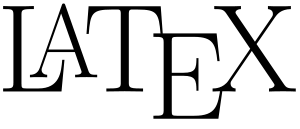
\includegraphics[width=4cm]{logo}}
\fi

%\renewcommand{\submittedtext}{change the default text here if needed}
\degree{Philosophi\ae Doctor (PhD), DPhil,..}
\degreedate{June, 2021}


% ----------------------------------------------------------------------
       
% turn of those nasty overfull and underfull hboxes
%\tolerance=1
%\emergencystretch=\maxdimen
%\hyphenpenalty=10000

\hbadness=10000
\hfuzz=50pt

\usepackage{enumitem}
\usepackage[table,xcdraw]{xcolor}
\usepackage{floatrow}
\usepackage{mathptmx}
\usepackage[T1]{fontenc}
\usepackage{textcomp}
\usepackage{listings}
\usepackage{tikz}
%\usepackage{paralist} 
\usepackage{import}

\usepackage{array}
\usepackage{color}
\usepackage{pgfplots}
\usepackage{amsmath}
\usepackage{xspace}
\usepackage{amssymb}
%\usepackage{enumerate}
%\usepackage{float}
%\usepackage{algpseudocode}
%\usepackage{algorithm}
\usepackage{verbatim}
\usepackage{multirow}
\usepackage{siunitx}
\usepackage{url}
\usepackage{chngcntr}
\usepackage{amsthm}
\usepackage{latexsym}
\usepackage{subfig}
\usepackage{pifont}
\usepackage{graphicx}
\usepackage{caption}
\usepackage{adjustbox} 
\usepackage{rotating}
%\usepackage{subcaption}
%\captionsetup{compatibility=false}
\usepackage{bibentry}
\usepackage{mathtools}
\usepackage{algorithm}
\usepackage{algorithmic}

\usepackage{ctable}

\usepackage[htt]{hyphenat}
\usetikzlibrary{patterns}
\counterwithout{footnote}{chapter}


%%<ALVARO>

\newcommand*\rot{\rotatebox{75}}
\newcommand*\OK{\ding{51}}
\newcommand{\argmax}[1]{\underset{#1}{\operatorname{arg}\,\operatorname{max}}\;}
\DeclarePairedDelimiter\ceil{\lceil}{\rceil}
\DeclarePairedDelimiter\floor{\lfloor}{\rfloor}

\newcounter{groupcount}
\pgfplotsset{
    draw group line/.style n args={5}{
        after end axis/.append code={
            \setcounter{groupcount}{0}
            \pgfplotstableforeachcolumnelement{#1}\of\datatable\as\cell{%
                \def\temp{#2}
                \ifx\temp\cell
                    \ifnum\thegroupcount=0
                        \stepcounter{groupcount}
                        \pgfplotstablegetelem{\pgfplotstablerow}{[index]0}\of\datatable
                        \coordinate [yshift=#4] (startgroup) at (axis cs:\pgfplotsretval,0);
                    \else
                        \pgfplotstablegetelem{\pgfplotstablerow}{[index]0}\of\datatable
                        \coordinate [yshift=#4] (endgroup) at (axis cs:\pgfplotsretval,0);
                    \fi
                \else
                    \ifnum\thegroupcount=1
                        \setcounter{groupcount}{0}
                        \draw [
                            shorten >=-#5,
                            shorten <=-#5
                        ] (startgroup) -- node [anchor=north] {#3} (endgroup);
                    \fi
                \fi
            }
            \ifnum\thegroupcount=1
                        \setcounter{groupcount}{0}
                        \draw [
                            shorten >=-#5,
                            shorten <=-#5
                        ] (startgroup) -- node [anchor=north] {#3} (endgroup);
            \fi
        }
    }
}




%%<IDAFEN>
\usepackage{xcolor}
\usepackage{color}
\definecolor{mygray}{rgb}{0.5,0.5,0.5}
\newcommand{\dfp}{dispel4py}

%\lstset{
%	basicstyle=\footnotesize,
%	breakatwhitespace=true,
%	breaklines=true,
%	numberstyle=\tiny\color{mygray},
%	numbers=left,
%	xleftmargin=1.5em,
%	frame=single,
%	framexleftmargin=1em,
%	frame=bt,
%}

%%subindex


\usepackage{multirow}

%%highlighting package
\usepackage{color}\newcommand{\mynote}[2][inline]{\color{red} [PENDING]: #2\color{black}}

%\newcommand{\mymark}[1]{\colorbox{orange}{#1}}
\newcommand{\mymark}[2][inline]{\color{orange}#2\color{black}}
\newcommand{\new}[2][inline]{\color{black}#2\color{black}}
\newcommand{\newtwo}[2][inline]{\color{black}#2\color{black}}
%\newcommand{\mynote}[2][inline]{\color{red} [PENDING]: #2\color{black}}
\usepackage{epigraph}
%%adding subsubsections
%\setcounter{secnumdepth}{3}

%%</IDAFEN>

\DeclareCaptionFormat{algor}{%
  \hrulefill\par\offinterlineskip\vskip1pt%
    \textbf{#1#2}#3\offinterlineskip\hrulefill}
\DeclareCaptionStyle{algori}{singlelinecheck=off,format=algor,labelsep=space}
%\captionsetup[algorithm]{style=algori}

\pdfoptionpdfminorversion 6

%% PIERRE

\definecolor{s1}{RGB}{228, 26, 28}
\definecolor{s2}{RGB}{55, 126, 184}
\definecolor{s3}{RGB}{77, 175, 74}
\definecolor{s4}{RGB}{152, 78, 163}
\definecolor{s5}{RGB}{255, 127, 0}
\definecolor{s6}{RGB}{160, 82, 45}

\pgfplotscreateplotcyclelist{tyr}{%
    s1,every mark/.append style={fill=white},mark=*\\%
    s2,every mark/.append style={fill=white},mark=square*\\%
    s3,every mark/.append style={fill=white},mark=diamond*\\%
    s4,every mark/.append style={fill=white},mark=triangle*\\%
    s5,every mark/.append style={fill=white},mark=pentagon*\\%
    s6,every mark/.append style={fill=white},mark=otimes*\\%
}

\pgfplotsset{compat=1.11,
    /pgfplots/ybar legend/.style={
    /pgfplots/legend image code/.code={%
       \draw[##1,/tikz/.cd,yshift=-0.25em]
        (0cm,0cm) rectangle (6.5pt,0.7em);},
   },
}

\pgfplotsset{
    grid=major,
    width=9cm,
    height=6cm,
    compat=1.9
}

\makeatletter
\g@addto@macro\@floatboxreset\centering
\makeatother

\pgfplotsset{plot coordinates/math parser=false}


\makeatletter
\pgfplotsset{
    groupplot xlabel/.initial={},
    every groupplot x label/.style={
        at={($({group c1r\pgfplots@group@rows.west}|-{group c1r\pgfplots@group@rows.outer south})!0.5!({group c\pgfplots@group@columns r\pgfplots@group@rows.east}|-{group c\pgfplots@group@columns r\pgfplots@group@rows.outer south})$)},
        anchor=north,
    },
    groupplot ylabel/.initial={},
    every groupplot y label/.style={
            rotate=90,
        at={($({group c1r1.north}-|{group c1r1.outer
west})!0.5!({group c1r\pgfplots@group@rows.south}-|{group c1r\pgfplots@group@rows.outer west})$)},
        anchor=south
    },
    execute at end groupplot/.code={%
      \node [/pgfplots/every groupplot x label]
{\pgfkeysvalueof{/pgfplots/groupplot xlabel}};  
      \node [/pgfplots/every groupplot y label] 
{\pgfkeysvalueof{/pgfplots/groupplot ylabel}};  
    },
    group/only outer labels/.style =
{
group/every plot/.code = {%
    \ifnum\pgfplots@group@current@row=\pgfplots@group@rows\else%
        \pgfkeys{xticklabels = {}, xlabel = {}}\fi%
    \ifnum\pgfplots@group@current@column=1\else%
        \pgfkeys{yticklabels = {}, ylabel = {}}\fi%
}
}
}

\def\endpgfplots@environment@groupplot{%
    \endpgfplots@environment@opt%
    \pgfkeys{/pgfplots/execute at end groupplot}%
    \endgroup%
}
\makeatother

\definecolor{gray}{rgb}{0.95,0.95,0.95}

\usetikzlibrary{arrows, positioning, shapes.multipart, calc, fit, patterns, decorations.text,
decorations.pathreplacing, shapes.symbols}
\usepgfplotslibrary{groupplots}

%% Tables

\newcommand{\specialcell}[2][c]{%
  \begin{tabular}[#1]{@{}c@{}}#2\end{tabular}}
  
\newcolumntype{P}[1]{>{\centering\arraybackslash}p{#1}}
\newcolumntype{M}[1]{>{\centering\arraybackslash}m{#1}}
\newcolumntype{N}{@{}m{0pt}@{}}

%% Algo

\renewcommand{\algorithmicrequire}{\textbf{Input:}}
\renewcommand{\algorithmicensure}{\textbf{Output:}}
\let\oldReturn\Return
%\renewcommand{\Return}{\State\oldReturn}
%\renewcommand{\algorithmicforall}{\textbf{for each}}

%\algnewcommand{\LineComment}[1]{\State{\textit{\textcolor{black!60}{\(\triangleright\) #1}}}}

%% PGF

\pgfdeclarelayer{bg}
\pgfdeclarelayer{mbg}
\pgfsetlayers{bg,mbg,main}

%% Sections

\newcommand{\lsection}[2]{
    \section{#2}
    \label{sec:#1}
}

\newcommand{\lsubsection}[2]{
    \subsection{#2}
    \label{sec:#1}
}

\newcommand{\lsubsubsection}[2]{
    \subsubsection{#2}
    \label{sec:#1}
}

\newcommand{\lsecref}[1]{\ref{sec:#1}}

\newcommand{\csubfloat}[2][]{%
  \makebox[0pt]{\subfloat[#1]{#2}}%
}
\newcommand{\centerhfill}[1][\quad]{\hspace{\stretch{0.5}}#1\hspace{\stretch{0.5}}}

\makeatletter
\newcommand\resetstackedplots{
\makeatletter
\pgfplots@stacked@isfirstplottrue
\makeatother
\addplot [forget plot,draw=none] coordinates{(1,0) (2,0) (3,0)};
}

%% /PIERRE

%: --------------------------------------------------------------
%:                  FRONT MATTER: dedications, abstract,..
% --------------------------------------------------------------

\begin{document}

%\language{english}

% sets line spacing
\renewcommand\baselinestretch{1.2}
\baselineskip=18pt plus1pt

\theoremstyle{plain}
\newtheorem{thm}{Theorem}[chapter] % reset theorem numbering for each chapter


\theoremstyle{definition}
\newtheorem{definition}[thm]{Definition} % definition numbers are dependent on theorem numbers

\newcommand{\attention}[1]{{\color{red}\textbf{#1}}}

\renewcommand\appendixname{ANNEX}


%: ----------------------- generate cover page ------------------------
\frontmatter
\maketitle  % command to print the title page with above variables


%: ----------------------- cover page back side ------------------------
% Your research institution may require reviewer names, etc.
% This cover back side is required by Dresden Med Fac; uncomment if needed.

% ALVARO: I'll have to change this

%\newpage
\pagestyle{plain}
\cleardoublepage
\pagestyle{plain}


\noindent Tribunal nombrado por el Sr. Rector Magfco. de la Universidad Polit\'{e}cnica de
Madrid, el d\'{i}a 9 de Junio de 2021. %\mynote{DD de YYYY de 2015}

\vspace{10mm}
Presidente:\hspace{0.3mm} Dr. Marcelo Arenas

\vspace{5mm}
Vocal: \hspace{6.7mm} Dr. Juan Sequeda 

\vspace{5mm}
Vocal: \hspace{6.7mm} Dra. Anastasia Dimou

\vspace{5mm}
Vocal: \hspace{6.7mm} Dr. Álvaro Sicilia Gómez 


\vspace{5mm}
Secretario:\hspace{0.67mm} Dr. Raúl García Castro

\vspace{5mm}
Suplente: \hspace{1.5mm} Dr. Mariano Fernández López   

\vspace{5mm}
Suplente: \hspace{1.5mm} Dr. Alberto Bugarín Díz

\vspace{10mm}
\noindent Realizado el acto de defensa y lectura de la Tesis el d\'{i}a 28 de Junio de 2021 en la Escuela T\'ecnica Superior de Ingenieros Inform\'aticos

\vspace{5mm}
\noindent Calificaci\'{o}n: \rule{123mm}{0.2mm}
\vspace{20mm}

EL PRESIDENTE \hspace{30mm} VOCAL 1 \hspace{30mm} VOCAL 2

\vspace{30mm}
%\begin{center}
\hspace{15mm} VOCAL 3 \hspace{45mm} EL SECRETARIO
%\end{center}




%: ----------------------- tie in front matter ------------------------

%\frontmatter
\cleardoublepage
% Thesis Dedictation ---------------------------------------------------

\begin{dedication} %this creates the heading for the dedication page



\end{dedication}

% ----------------------------------------------------------------------
\cleardoublepage

\begin{acknowledgementslong} 

Realizar un trabajo de investigación complejo, como es el caso de una tesis doctoral, no se puede entender sino como un trabajo colaborativo. Por ello,  a lo largo de las líneas que siguen trataré de agradecer y mencionar a todo aquel que ha contribuido, de una forma u otra, al desarrollo de esta investigación.

Para comenzar, la realización de esta tesis habría sido imposible sin el apoyo constante de dos personas que admiro profundamente desde el primer momento en que las conocí y a las que considero mis dos padrinos académicos, Oscar Corcho y Maria-Esther Vidal.  Gracias, Oscar, por haberme dado la posibilidad de realizar este trabajo bajo tu supervisión en el Ontology Engineering Group (OEG). Además de disfrutar enormemente con las discusiones que hemos ido teniendo a lo largo de estos cinco años, me gustaría agradecerte la confianza que depositaste en mí y la libertad que me has otorgado, quizá un poco difícil de gestionar y comprender al comienzo por mi parte, pero sin la que  no habría crecido personal y profesionalmente de la manera que lo he hecho. Al final, el tiempo pone a cada uno en el lugar que le corresponde. Gracias por tu paciencia y continuo optimismo, que me han ayudado a \textit{``ver siempre el lado bueno de la vida''} (como cantaban los \textit{Monthy Python} en ``La Vida de Brian''), tan necesario en los momentos complicados y, particularmente, en los tiempos que corren. De Maria-Esther admiro su pasión por el trabajo; con ella aprendí a creer en lo que uno hace,  a valorar el trabajo de investigación. Nunca sabré cómo agradecerte el trato recibido, como si fuese uno más de tus estudiantes, durante mi estancia en SDM, así como tu contribución todo el trabajo que hemos realizado juntos durante la segunda parte de mi doctorado. Es complicado expresar en tan pocas líneas el completo y desinteresado apoyo que he recibido por tu parte, así como los valores y enseñanzas sobre el esfuerzo, la perfección en el trabajo y tu entusiasmo por todo lo que haces. Simplemente, gracias. 

El sentimiento de pertenencia a un grupo es otra de las claves para poder llegar a completar una tesis con éxito. Más que un grupo, creo que el OEG es una familia, una gran familia. Esta tesis no habría sido lo mismo sin las enriquecedoras discusiones y charlas que he tenido con mis ``hermanos'', Paola y Carlos, sobre el doctorado, la investigación y la vida en general. Gracias al resto de doctorandos (o doctores ya): Alba, Serge, Elvi, Pablo, Julia, etc, a los ``seniors'' del OEG y ex-OEGs: Esteban, Raúl Alcazar, Vicky, Raúl García, JARG, Ana Ibarrola, Elena, Miguel Ángel, Paco, Maria Poveda, Idafen, José Luis, etc. Gracias a Juan y Alvaro, dos personas con las que he compartido mucho (también cervezas) durante estos años y que me han ayudado a madurar; me llevo conmigo dos grandes amistades. Especialmente, quiero agradecer su apoyo a Patricia, mi ``compi' de batallas en la vida, de viajes en el coche, de charlas interminables, del ``siempre hay que decir sí a todo'', de las idas y venidas, y las noches madrileñas hasta el amanecer. Asimismo, ha sido un gusto compartir tiempo y experiencias con todos los integrantes del grupo de integración de datos. Me gustaría agradecer también a Edna su ayuda en los artículos que hemos escrito juntos y su paciencia durante la revisión de esta tesis. Freddy, gracias por tus ideas locas y tu buen humor. Jhon, Ana, Luis, Dani, Julián, Ahmad, Marlene y Andrea, he disfrutado enormemente discutiendo, definiendo y logrando retos con todos vosotros. 

To the people from Ghent, especially to Pieter and Anastasia, my ``postdocs'' in the shadows. Thanks for giving me the possibility to work and collaborate with you and your teams, especially to Ben, Pieter and Julián. Hope that this is only a promising beginning. Lucie and Sam, I am extremely glad to meet you, first in Bertinoro, and then in Hannover. Lucie, you were my support during the good and bad moments of my internship in Germany. I am really happy to have a friend like you in my life. Sam, I am never going to forget our legendary week in Rodhes and all the awesome things that came after it. I really admire your passion and I enjoyed working with you; you will be a reference researcher for many people. Finally, to the rest of the SDM-TIB family: Enrique, Kemele, Ahmad, Ariam, Maria Isabel...

E por último, pero non menos importante, quero dar as grazas  a miña xente de sempre, aos meus galegos. A meus pais, que foron unha continua axuda durante  esta longa viaxe; deles quédome coa súa forza para afrontar os momentos delicados e coa paixón coa que confrontan o día a día. Mamá, grazas por todas as discusións e o teu punto de vista sobre que é un bo investigador; eres un referente para min. Papá, ogallá algún día poda desfrutar de cada momento coa mesma intensidade e ledicia coa que o fas ti. Martín, meu irmán, creo que aínda que en diferentes etapas da vida, durante estes anos os nosos camiños xuntáronse pouco a pouco, e o teu apoio incondicional sempre foi de gran axuda. Gracias aos meus amigos de sempre: Rafa, Marta, Clau, Paula, Erle, Ánxela, Carme, Olga e Minia... Pero tamén aos que atopei en Madrid: Santi, Patricia, Pamela, Carolina... Sempre conseguiron sacarme un sonriso e fixéronme ver que a academia e a universidad non son o único que existe. Nada sería igual de non ser por eles.

Las últimas líneas van dedicadas a toda esa gente que me ha ayudado, muchas veces sin saberlo, a conseguir esta meta. Las largas mañanas de experimentación con 180º y Virginia Díez, las tardes-noches de tenis con Rafa, Iñaki y Andrés, entre otros; la última temporada escribiendo la tesis en el piso de Madrid y saliendo a ``rodar'' unos kilómetros con Ismael; gracias a todos los estudiantes que han participado en alguna edición del Open Summer of Code Spain. Gracias, Jorge, por tu hospitalidad y amistad durante mi estancia en Santiago de Chile.

Por encima de todo, gracias por hacerme sentir en casa.

\vspace{10mm}

\textit{
\null\hfill Vuelvo a casa \\
\null\hfill De la zozobra de mi corazón \\
\null\hfill Ahora vivo aquí \\
\null\hfill Pensé que estaba solo y descubrí \\
\null\hfill Que estaban todos los que importan \vspace{6mm} \\
} 
\null\hfill Iván Ferreiro - Casa, ahora vivo aquí

\end{acknowledgementslong}












%: ----------------------- abstract ------------------------

% Your institution may have specific regulations if you need an abstract and where it is to be placed in the document. The default here is just after title.
\cleardoublepage

% Thesis Abstract -----------------------------------------------------


\begin{abstractslong}    

\end{abstractslong}

\cleardoublepage
\begin{abstractslongSpanish}




\end{abstractslongSpanish}
% ---------------------------------------------------------------------- 


% The original template provides and abstractseparate environment, if your institution requires them to be separate. I think it's easier to print the abstract from the complete thesis by restricting printing to the relevant page.
% \begin{abstractseparate}
%   
% Thesis Abstract -----------------------------------------------------


\begin{abstractslong}    

\end{abstractslong}

\cleardoublepage
\begin{abstractslongSpanish}




\end{abstractslongSpanish}
% ---------------------------------------------------------------------- 

% \end{abstractseparate}


%: ----------------------- contents ------------------------
\cleardoublepage
\setcounter{secnumdepth}{3} % organisational level that receives a numbers
\setcounter{tocdepth}{2}    % print table of contents for level 3
\tableofcontents           % print the table of contents
% levels are: 0 - chapter, 1 - section, 2 - subsection, 3 - subsection


%: ----------------------- list of figures/tables ------------------------

\listoffigures	% print list of figures

\listoftables  % print list of tables

\listofalgorithms % Print list of algorithms


%: ----------------------- glossary ------------------------

% Tie in external source file for definitions: /0_frontmatter/glossary.tex
% Glossary entries can also be defined in the main text. See glossary.tex

%% this file is called up by thesis.tex
% content in this file will be fed into the main document

% Glossary entries are defined with the command \nomenclature{1}{2}
% 1 = Entry name, e.g. abbreviation; 2 = Explanation
% You can place all explanations in this separate file or declare them in the middle of the text. Either way they will be collected in the glossary.

% required to print nomenclature name to page header
\markboth{\MakeUppercase{\nomname}}{\MakeUppercase{\nomname}}


% ----------------------- contents from here ------------------------

% chemicals
%\nomenclature{DAPI}{4',6-diamidino-2-phenylindole; a fluorescent stain that binds strongly to DNA and serves to marks the nucleus in fluorescence microscopy} 
%\nomenclature{DEPC}{diethyl-pyro-carbonate; used to remove RNA-degrading enzymes (RNAases) from water and laboratory utensils}
%\nomenclature{DMSO}{dimethyl sulfoxide; organic solvent, readily passes through skin, cryoprotectant in cell culture}
%\nomenclature{EDTA}{Ethylene-diamine-tetraacetic acid; a chelating (two-pronged) molecule used to sequester most divalent (or trivalent) metal ions, such as calcium (Ca$^{2+}$) and magnesium (Mg$^{2+}$), copper (Cu$^{2+}$), or iron (Fe$^{2+}$ / Fe$^{3+}$)}



 
%
%\begin{multicols}{2} % \begin{multicols}{#columns}[header text][space]
%\begin{footnotesize} % scriptsize(7) < footnotesize(8) < small (9) < normal (10)
%
%\printnomenclature[1.5cm] % [] = distance between entry and description
%\label{nom} % target name for links to glossary
%
%\end{footnotesize}
%\end{multicols}



%: --------------------------------------------------------------
%:                  MAIN DOCUMENT SECTION
% --------------------------------------------------------------

% the main text starts here with the introduction, 1st chapter,...
\mainmatter

%\renewcommand{\chaptername}{} % uncomment to print only "1" not "Chapter 1"
%\titleformat{\chapter}[display]{\normalfont\bfseries\}{\chaptertitlename\ \thechapter}{5pt}{\Huge}

%-#####-> Uncomment to have Andres' style for chapter title

%\titleformat{\chapter}[display]
%{\bfseries\Large}
%{\filleft\MakeUppercase{\chaptertitlename} \Huge\thechapter}
%{4ex}
%{\titlerule
%\vspace{2ex}%
%\filright}
%[\vspace{2ex}%
%\titlerule]

%-#####-> End uncomment



% this file is called up by thesis.tex
% content in this file will be fed into the main document

%: ----------------------- introduction file header -----------------------
\chapter{Introduction}
\label{chap:intro}

\epigraph{All human things are subject to decay, and when fate 
summons, Monarchs must obey}{\textit{Mac Flecknoe \\ John Dryden}}

\section{Thesis Structure}
\label{sec:thesisstructure}



\section{Dissemination Results}
\label{sec:disresults}





\chapter{State of the Art}
\label{chap:soa}

In this chapter, we introduce the current state of the art in knowledge graph construction using declarative mapping rules. We provide an overview of approaches, techniques and methodologies for constructing and querying (virtual) knowledge graphs based on semantic web technologies. We describe the declarative annotations and mapping languages specifications that have been proposed to construct these kind of data models together with their main benefits. Finally, we present the current methodologies to evaluate the quality of knowledge graph construction engines such as benchmarkings and test-cases.


\section{Ontology-Based Data Access and Integration}


\section{Representation and Query Language for the Semantic Web}

\subsection{RDF: Resource Description Framework}

\subsection{SPARQL}




\section{Annotations in Knowledge Graph Construction}
One of the main components for the construction of knowledge graphs are the annotations. Additionally to the mapping rules, that relate the target model with the input sources in a typical data integration system definition, we include in the annotations set the constraints concept. In a DIS, the constrains property allows to: i) define ad-hoc transformation functions that permit the cleaning and preparation of the input data; ii) definition of metadata annotations to describe the content of the input source. This property is essential during a knowledge graph construction process as it is able to deal with the typical features of heterogeneous data sources such as the absence of a well-defined and fixed data schema, a normalized database instance or the non-explicit declarations of relations among the sources. We start this section discussing existing approaches for the design of mappings. Then, we describe the current mapping language specifications and their standardization through the W3C. Finally, we present approaches to define, declaratively, constraints over a DIS.

\subsection{Mapping Rules}
The mapping layer contains information about how the input sources are related with the target model. There are two basic approaches for defining mapping rules in a data integration system: Local as a View (LAV) and Global as a View (GAV). In semantic web, the usual followed approach to define this rules is the Global as View one. We now provide a description of each proposals more in detail.

\subsubsection{Local as a View Mapping rules (LAV)}
In \citep{ullman1997information} the elements of the source schema $S$ are mapped  to a query $Q_G$ over the target schema $G$. The main benefits of this approach is that it supports continuous changes of the source schema (e.g., adding new sources or modify their underlying representation) since there is no need to change the query processing component. Thus, LAV is usually useful when the global schema $G$ is stable but the local schema $S$ may suffer modifications over the time.


ToDo: ADD EXAMPLE

\subsubsection{Global as a View Mapping Rules (GAV)}
In \citep{halevy2001answering} each element of the global schema $G$ is mapped to a query over $Q_S$ the source schema $S$. 


\subsubsection{R2RML: W3C Recommendation}

\subsubsection{RML: Extending R2RML for Heterogeneous Data}

\subsection{Declarative Constraints: Transformation Functions and Metadata}

\subsubsection{Transformation Functions in Mappings}

\subsubsection{Metadata for data on the web}


\section{Knowledge Graph Construction Engines}

\section{Evaluation of Knowledge Graph Construction}

\subsection{Test-Cases}
\subsection{Benchmarks}



\section{Conclusions}



\chapter{Objectives and Contributions}
\label{chap:objectives}
The main goal of this work is the use of declarative mapping rules and their knowledge encoded for the construction and evaluation of knowledge graphs from heterogeneous data sources. This chapter presents the objectives and contributions to the state of the art of our work. Additionally, we detail the assumptions considered when we started this work, hypothesis and restrictions that delimit and describe the scope of this thesis.

\section{Objectives}
In the context of this thesis we identify two different goals. First, we provide a definition and a set of properties over the new concept of \textit{mapping translation} and we describe two approaches that take into account this concept to improve the construction and access of knowledge graphs from heterogeneous data sources. The second goal of the thesis consists in define the main steps and resources for an objective and proper evaluation of these kind of approaches.

In order to achieve the first objective of this thesis, the open research problems that have to be solved are:

\begin{itemize}
    \item The construction of knowledge graphs (virtual or materialized) from heterogeneous data sources using declarative mapping rules is still an open issue in the state of the art. Based on the W3C recommendation R2RML~\citep{R2RML}, and with the aim of providing support to other format beyond relational databases, many new declarative mapping languages are proposed such as RML~\citep{dimou2014rml}, xR2RML~\citep{michel2015translation}, KR2RML~\citep{slepicka2015kr2rml}, CSVW~\citep{tennison2015model}, or D2RML~\citep{chortaras2018mapping}.Many of these extensions are proposed with the aim of solving specific heterogeneity issues of the input data, hence, they start to lose their generalization and the benefit of the declarative approach of the rules. To deal with these problems, we propose the possibility of the translation among these different languages, covering at least those common characteristics that are shared across languages, introducing one of the main ideas about a new generation of knowledge graph construction approaches.
    \item The construction of virtualized knowledge graphs from raw data (e.g., CSV, JSON or XML) has been tackle as an engineering process delegating the management of these data sources to databases such as Apache Drill\footnote{\url{https://drill.apache.org/}} and Spark-SQL\footnote{\url{https://spark.apache.org/sql/}}. These systems allow the generation of a simple relational database layer over the input data sources. However, in order to tackle the advantage of proposed SPARQL-to-SQL optimization techniques~\citep{priyatna2014formalisation,calvanese2017ontop}, a well-formed RDB is required, including its corresponding constraints. Focused on the specific case of tabular data, we propose a framework that exploits mapping rules and metadata annotation to deal with the typical heterogeneity issues on querying these datasets under an OBDA environment. Its main aim is to improve query evaluation performance, as well as query completeness.
    \item Multiple types of query interfaces have been proposed to query heterogeneous data on the web. GraphQL~\citep{graphql} aims to solve problems such as under/over fetching of other common used interfaces such as REST APIs. Although this specification has been widely included by multiple organizations in their systems as a query layer
    \end{itemize}

The second goal (methodologies for a proper evaluation of knowledge graph construction systems) have the following open problems:
\begin{itemize}
    \item 
\end{itemize}
. We depict in Chapter \ref{chap:soa} that there is not an standard and homogenize manner to evaluate these systems. They do not taking into account relevant parameters that can impact in their behaviour or they are only based on one data format and fixed distributions.


\section{Contributions to the State of the Art}

\section{Assumptions}

\section{Hypothesis}

\section{Restrictions}



\chapter{A New Generation of Knowledge Graph Construction Engines}
\label{chapter:mappig-translation}

\epigraph{The primary goal of a researcher should be to continually challenge science with creative ideas}{\textit{Oscar Corcho}}


Database technologies play a vital role in the development of information systems for all sorts of organizations. So far, relational databases (RDB) are still the dominating type of structure and technology used for data management inside organizations, although other formats (e.g. JSON, spreadsheets, XML) and types of databases (e.g. noSQL, graph databases) have also emerged as alternatives for data representation and management in the last decades. 

\begin{figure*}[!ht]
    \centering
    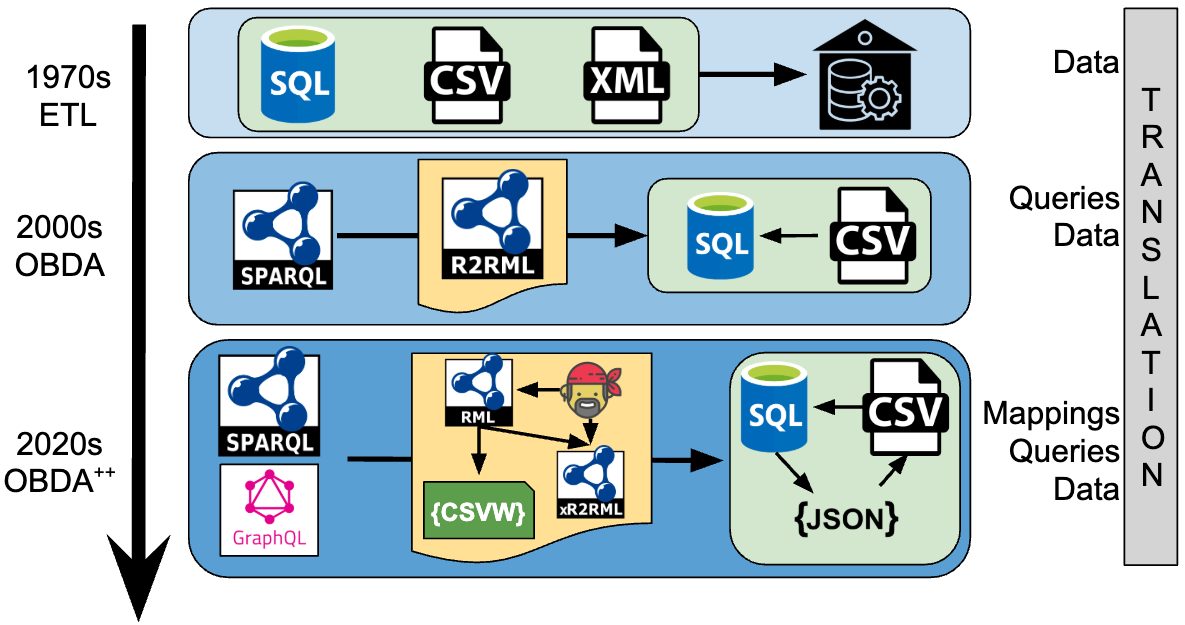
\includegraphics[width=1\columnwidth]{./figures/mt_obda_timeline.png}
    \caption[Timeline of data integration techniques]{\textbf{Timeline of data integration techniques}. During the 1970s ETL approaches started with data translation techniques, current generation of KGC incorporated techniques for query translation and next generation of KGC systems which mapping translation approaches are to be applied.
    }
    \label{fig:obdatimeline}
\end{figure*}

In the early days of information system development, it was natural for organizations to develop their own data models, which were strongly aligned with their activities. This led to a large heterogeneity of data models across organizations, and even across different departments inside the same organization. Such heterogeneity was especially evident in the case of organizational changes, merges, etc. These situations made researchers and professionals start working on solutions for data integration, where data from several sources needed to be accessible according to a unified and global view over such local heterogeneous data sources. Data warehouses were used in order to align and materialize data from different sources, normally from the same organization, so as to provide support for analytical queries and for the generation of reports. Popular technologies used in production systems worldwide included the use of Extract-Transform-Load (ETL) workflows to overcome heterogeneity and ensure the availability of data in such data warehouses or on integrated databases. Indeed, these approaches are still strongly used nowadays.

In the meantime, data integration challenges became even more relevant when organizations started using Web technologies to provide access to their data (via Web Services, REST APIs or using Semantic Web and Linked Data approaches), both for their own information system development as well as for data sharing, and later on when public administrations started publishing open data according to  public-sector information reuse initiatives. Availability and heterogeneity of data (both in terms of content and format) is nowadays present at an unprecedented level. Following the aforementioned ETL approaches, the term data lake has been rather recently coined to refer to an evolution of data warehouses that considers not only structured data but also the other types of (semi-)structured and unstructured formats in which data is made available nowadays, as discussed above.

Over these decades, several approaches have been proposed to tackle data integration challenges. We are specially interested in those that fall under the area of Ontology Based Data Access (OBDA) and Integration (OBDI)~\citep{poggi2008linking}, which is recently also defined as Knowledge Graph Construction (KGC) methods. From now on we will refer to all of them, in a general manner, as KGC. As we have already mentioned in Chapter \ref{chap:intro} and Chapter \ref{chap:soa}, in KGC, ontologies are used as a global view over heterogeneous data sources and mappings are used to describe such relationships in a declarative manner. Many different types of KGC mapping languages have been proposed over the last decades, with a large variety of syntax and formats especially in the early ones. Since the standardization of languages like RDF and OWL, several languages were proposed focused on the transformation from relational databases into RDF (e.g. D2R~\citep{bizer2004d2rq}, R2O~\citep{barrasa2004r2o}). This led to the creation of the RDB2RDF W3C Working Group, which published two recommendations for transforming the content of relational databases into RDF: Direct Mapping \citep{arenas2013direct} and R2RML \citep{R2RML}.

As we describe in Chapter \ref{chap:soa}, a bit after R2RML was recommended, and because of its use in different types of contexts, new needs and requirements arose, especially in relation to supporting other formats beyond relational databases, and this resulted in the creation of many new mapping languages, such as RML \citep{dimou2014rml} (to deal with CSVs, JSON and XML data sources), xR2RML \citep{michel2015translation} (to deal with MongoDB), KR2RML \citep{slepicka2015kr2rml} (to deal with nested data), CSVW\footnote{\url{https://www.w3.org/ns/csvw}} (to describe CSV files on the Web), or D2RML \citep{chortaras2018d2rml} (for XML, JSON and REST/SPARQL endpoints). In addition to declarative languages, non-declarative mapping languages have also been proposed, such as SPARQL-Generate \citep{lefranccois2017sparql}, Helio\footnote{\url{https://helio.linkeddata.es/}},  TARQL\footnote{\url{https://github.com/tarql/tarql}} or Triplify~\citep{auer2009triplify}.

\noindent\paragraph{\textbf{Why so many mapping languages?}}
There are several reasons why new mapping languages are needed. The first and main reason is that a typical mapping language is designed to work with a specific \textbf{data format} (e.g. R2RML is focused on relational databases). Even for a more generic-purpose mapping language, such as RML, there may still be a need to extend it to support a more specific technology, such as nested data hierarchies. Another reason is \textbf{readability and compactness}. Most mapping languages are designed in a format to be parsed by machines and they do not take into account human readability. Examples of languages created to account for this are R2RML-Iterator (for statistical CSV files) \citep{chaves2018virtual} or YARRRML \citep{Heyvaert2018Declarative}. Lastly, many of existing mapping languages \textbf{lack formalization}, making it difficult to apply, for example, query translation techniques. 

Therefore, the current situation of a KG construction practitioner that needs to provide access to a varied set of heterogeneous data sources is that there are many different options to select from, and it is difficult to determine which one is better for each situation. Languages are not necessarily interoperable, and many of them come associated with a very specific engine that supports them. At the same time, it is clear that most of these languages share many common aspects, such as the description of where the data comes from, how IRIs can be created for resources, how triples need to be generated (in a materialized or virtual way), etc. Having the possibility of translating among these different languages, covering at least those common characteristics that are shared across languages, would allow practitioners to have the possibility of selecting a wider set of engines to implement their KG construction system, or the different parts of a KG.

In this chapter, we lay out our vision that the next generation of KGC systems should take advantage of this proliferation of mapping languages. In other words, in addition to the data translation and query translation techniques that have been widely addressed in the state of the art of KGC so far, the KGC research community will need to think carefully about how to address mapping translation (See Figure \ref{fig:obdatimeline}), as we describe in the next sections.


\section{Mapping Translation: Concept Definition}
We define the mapping translation concept as a function that transforms a set of mappings described in one language (we call them original mappings) into a set of mappings described in another language (we call them target mappings). 

Our next step is to attach desirable properties for such a function. In this line, we propose to use and adapt some properties that have been described by \citep{sequeda2012directly} and \citep{hartig2017foundations} in their works. To be more specific, those properties are \textit{information preservation} and \textit{query result preservation} (Figure \ref{fig:mt}).

The \textbf{Information Preservation Property (IPP)} applied to a mapping translation function states that at least there is a function so that its application over the information generated by the application of the target mappings over the original data source returns the same information generated by the application of the original mappings over the same data source.

The \textbf{Query Result Preservation Property (QRPP)} applied to a mapping translation function states that for any query that can be evaluated over the information generated from the application of the original mappings to the original data source, there is at least a function to generate another query that can be evaluated over the information generated by the application of the target mappings to the same data source, in such a way that both queries return the same results.


Finally, using these two properties, we define the concepts of weak and strong semantics preservation for a mapping translation function, as follows: a mapping translation function exhibits \textbf{weak semantics preservation} if only IPP holds. If both IPP and QRPP are satisfied, then we say that it holds the \textbf{strong semantics preservation} property.


\begin{figure}[!t]
    \centering
    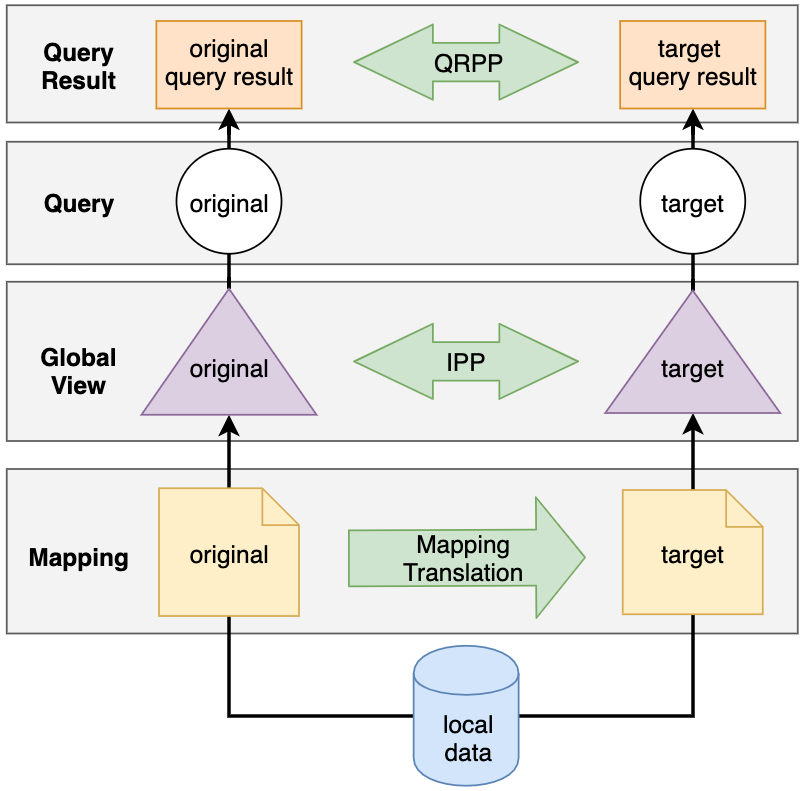
\includegraphics[width=0.6\columnwidth]{./figures/mapping-translator.png}
    \caption[Mapping translator properties]{\textbf{Mapping Translator Properties.} The results (triangles) may satisfy the IPP property after the application of the source and target mappings over the same data. In the same way, query results (rectangles) may satisfy the QRPP property when equivalent queries are evaluated over the source and target results.}
    \label{fig:mt}
\end{figure}


\section{Mapping Translation by example}
In this section we identify a set of scenarios and challenges in the creation and use of KGC mapping languages, where mapping translation is relevant. We describe the challenge and provide some references to some of the work presented in the literature addressing or acknowledging it. The presented use cases are summarized in Table \ref{tab:chap4_summary}.

\begin{table}[!ht]
\centering
\caption{Summary of Mapping Translation Approaches}
\label{tab:chap4_summary}
\resizebox{0.65\textwidth}{!}{%
\begin{tabular}{c|c|c}
\hline
\textbf{Use Case}         & \textbf{Engine} & \textbf{Translation}     \\ \hline
Maintenance               & Mapeathor       & Excel-to-[R2]RML           \\ \hline
Maintenance               & yarrrml-parser  & YARRRML-to-RML           \\ \hline
Maintenance               & r2rml-statistic & R2MLIterator-to-R2RML    \\ \hline
Maintenance               & ShExML          & ShExML-to-RML            \\ \hline
Declarative to Programmed & morph-graphQL   & R2RML-to-GraphQLResolver \\ \hline
Access                    & Morph-CSV       & RML(+FnO)-to-R2RML       \\ \hline
Optimizations                    & FunMap          & RML(+FnO)-to-RML          \\ \hline
Optimizations/Semantics   & ontop           & R2RML-to-OBDA            \\ \hline
\end{tabular}%
}
\end{table}



\subsection{Improving mapping creation and maintenance}

Creating and maintaining KGC mappings is usually difficult, since mapping languages have been created so that they can be consumed by the corresponding engines, and they commonly suffer from readability and compactness problems. With respect to \textbf{readability}, several approaches have focused on providing mapping editors (e.g. \citep{heyvaert2016rmleditor,iglesias2020mapeathor}) so that mappings are easier to create by non experts. However, these editors are usually limited to some features of the mapping language or to a specific version of the mapping language specification, and in general they still require knowledge about the underlying mapping language syntax. With respect to \textbf{compactness}, there are cases where the generated mapping documents are very long and repetitive, making it difficult to create and maintain~\citep{chaves2018virtual}. For instance, this is the case when a KGC approach is used to provide access to multidimensional data sources, such as the ones commonly used to publish statistical data. We describe three cases where mapping translation ideas are already being applied to address these issues. 

YARRRML~\citep{Heyvaert2018Declarative} is a serialisation of RML mappings that uses the YAML (a human-readable data serialization language) format\footnote{\url{https://yaml.org/}}. It is designed with the objective to reduce the size and verbosity of RML. There is no specific engine or parser to exploit YARRRML mappings in an KGC setting. Instead, the tool Matey\footnote{http://rml.io/yarrrml/matey/} is in charge of translating YARRRML mappings into RML, so that any RML-compliant OBDA engine can be used to exploit them. ShExML~\citep{garcia2020shexml} presents a similar work, where the authors extend the syntax of ShEx shapes constraints~\citep{prud2014shape} to support the construction of KGs from heterogeneous data sources. They conduct a user evaluation and observe that their approach is easy to use and maintain. To exploit all the benefits from the RML engines, they provide a translator engine from ShExML to RML.

In the case of multidimensional data (e.g. official statistics data), the W3C RDF DataCube recommendation is the ontology that is commonly used as a global view in an KGC setting. In most cases, the amount of mappings that would need to be created to link the original data source with the ontology will be rather large and with similar structure. Therefore, there is a high risk that the [R2]RML mapping document(s) generated in the end will contain clerical errors due to copy\&paste\&edit operations. Furthermore, they will be difficult to maintain. As a result, R2RML-Iterator~\citep{chaves2018virtual} is proposed as a simplified mapping language specifically designed for this type of data. The proposal is detailed in Section \ref{sec:chap4_rmlc}.


\subsection{From declarative mappings to programmed adapters}
Introduced in 2000, REST \citep{fielding2000architectural} has become now the most popular architecture for the provision of web services and the implementation of Web-based applications. However, the complexity of software development continues evolving, and aspects that received little attention, such as the size of data being exchanged/transmitted or the number of API calls being made, are now becoming more relevant in the context of mobile application development. As a result, problems like \textit{over-fetching} (a REST endpoint returns more data than what is required by the client) and \textit{under-fetching} (a single REST endpoint does not provide sufficient information requested by the client) are now being discussed. In order to address these problems, Facebook proposed the GraphQL query language \citep{graphql}, used internally since 2012 and released for public use in 2015. Since then it has been increasingly adopted, and GraphQL is now supported by multiple GraphQL engines for major programming languages (e.g. JavaScript, Python, Java, Golang, Ruby).

The two main components of a GraphQL server are the \textbf{schema} and the \textbf{resolvers}. The GraphQL schema specifies the type of an object together with the fields that can be queried. GraphQL resolvers are data extraction functions implemented in a programming language that are responsible to translate GraphQL queries into queries supported by the underlying datasets (e.g. GraphQL to SQL). In addition, query planning tools have been developed in order to translate GraphQL queries into other query languages (e.g. dataloader\footnote{\url{https://github.com/facebook/dataloader}}, joinmonster\footnote{\url{https://join-monster.readthedocs.io/en/latest/}}).

In a recent paper~\citep{priyatna2019morph} we proposed the use of the mapping translation concept to facilitate the generation of GraphQL resolvers. We propose specifying mappings in R2RML, which is a well-defined and formalized mapping language, and apply a mapping translation technique to generate automatically the corresponding GraphQL schemes and resolvers in different programming languages. Our intuition is that following this approach, GraphQL resolver will be easier to maintain, as they are declarative and independent from any programming language. The details of this approach are presented in Section \ref{chap6_morphgraphql}.

\subsection{Providing access to semi-structured data}
Semi-structured data formats are one of the most widely used formats to publish data on the Web. Although existing mapping languages provide support for this type of data sources, existing engines are mostly focused on the generation (materialization) of RDF-based knowledge graphs, with only a few proposals (e.g. xR2RML~\citep{michel2015translation}) focused on the application of query-translation techniques (virtualization) over such types of data sources.

In the specific case of spreadsheets (CSV), providing access to this format is difficult for two main reasons: (i) CSV does not provide its own query language, (ii) there are some transformations that are commonly needed when treating data available in CSVs. For solving the first issue, query translation techniques have been applied over such data format by considering a CSV file as a single table that can be loaded in an RDB. For the second issue, some extensions of well-known mapping languages (RML together with the Function Ontology~\citep{de2017declarative}) and annotations following the CSVW specification~\citep{tennison2015model} can be used.

Morph-CSV applies the concept of mapping translation for enhancing OBDA query translation over CSV files from SPARQL. It exploits the information of CSVW annotations and RML+FnO mappings to create an enriched RDB representation of the CSV files together with the corresponding R2RML mappings, allowing the use of existing query translation (SPARQL-to-SQL) techniques implemented in R2RML-compliant OBDA engines. This contribution is detailed in Section \ref{chap6_morphgcsv}.


\subsection{Understanding the semantics of mapping languages}
To the best of our knowledge, there has not been yet any formal study of the relationship between R2RML and the Direct Mapping recommendations, and among the many different mapping languages that have arisen recently.

For the first case (R2RML and Direct Mapping), intuitively we may consider that Direct Mapping is a subset of R2RML, given the expressive power provided by the latter. However, it would be interesting to know how expressive Direct Mapping may be in case that views are generated for the underlying data sources, for instance. Our intuition is that given the possibility of creating a database view from an existing database, there exists a fragment of R2RML that can be translated into Direct Mapping, such that the application of Direct Mapping over the view generates equivalent results as the application of R2RML mappings over the original database. Finding such fragment brings a practical implication because it would lower down the barrier for transforming data into RDF and enable people to use Direct Mapping engines, which are in general easier to use than R2RML engines for those people who are used to manage databases.

Similarly, this analysis may be extended to other combinations of mapping languages, so as to allow mapping translations among them that would allow exploiting the specific characteristics of each associated implementation, as well as describing formally their semantics, especially for those cases where no formal specification of the semantics has been provided yet.

Ontop \citep{rodriguez2015efficient} is an OBDA system that comes with both data and query translation techniques. Ontop translates R2RML mappings into its own mapping called ``OBDA mappings''. These mappings are represented as datalog rules, allowing the formalisation and semantic optimisation techniques to be performed, and generating a more efficient SQL queries (e.g. self-join elimination) that can be evaluated in less time by the underlying databases.


\section{Use Case: Virtual Knowledge Graph Construction in the Statistics Domain}
\label{sec:chap4_rmlc}

Statistics data is one of the most common ways of sharing public information nowadays. PDF, HTML and, especially, CSV format, are some of the most used formats of tabular data being published on the web by statistics agencies. Whereas this is still the main trend, many agencies worldwide are embracing semantic technologies for publishing their resources as Statistics Knowledge Graphs (SKG)\footnote{\url{https://semstats.org}}. In many cases both formats co-exist, allowing to access the information in different ways. 

Due to the high volume and variability of data, the transformation from tabular to SKG-oriented formats requires a process that is standard and maintainable. We identify two main approaches for transforming tabular data to Statistics Knowledge Graph (SKG). The first approach is an ad-hoc approach, such as one that has been reported in~\citep{corcho2017publishing}, in which CSV data is converted into RDF Data Cube~\citep{cyganiak2012rdf} using a set of custom rules. The second approach is defined on the basis of mapping languages, such as the RDB2RDF W3C Recommendation, R2RML, in which transformations are codified in a standard language, with several tools available for applying them.

In an ad-hoc approach~\citep{corcho2017publishing}, a processor which is the main component responsible for the transformation process, is developed for a specific purpose. Those processors are not commonly used for other solutions. The SKG resulting from the transformation process is stored in a triple store and there is a need for repeating the transformation process whenever the original statistics data changes to ensure that generated SKG is synchronised with the original statistics data. On the other hand, using R2RML to generate SKG brings several benefits in comparison to the ad-hoc approach. There are many R2RML processors~\citep{priyatna2014formalisation,calvanese2017ontop} available which means that one is not restricted to use a particular processor and may easily use another if necessary. Furthermore, many of those processors have incorporated techniques for keeping the desired SKG virtual, thus eliminating the need of synchronization between the tabular data and SKG. A virtualization process is highly recommended when the data published is volatile because it ensures that the retrieved data is updated. This is achieved by translating SPARQL queries posed to the virtual SKG into another query supported by the underlying data source and evaluated on the original dataset~\citep{poggi2008linking}. Table \ref{table:chapter4_compare} summarizes our discussion regarding the approaches on transforming statistics data into SKG.

\begin{table}[tbp]
\caption[KG Construction Approaches from Statistics Data]{Comparison of Approaches for Transforming Statistics Data to SKG}
\label{table:chapter4_compare}
\begin{tabular}{c|c|c}
\hline
\textbf{Features} & \textbf{Ad-Hoc~\citep{corcho2017publishing}}   & \textbf{R2RML~\citep{R2RML}}  \\ \hline
Processor Type    & Solution Specific & General Purpose \\ 
\# Processors     & 1                 & Many            \\
Materialization   & Yes               & Yes             \\ 
Virtualization    & No                & Yes             \\ \hline
\end{tabular}
\end{table}

The size of the R2RML mapping documents depends on the number of columns in the tabular data and number of dimensions to be generated. For example, a CSV file that contains data from all the European countries will need an R2RML mapping with one section defined the required dimensions for each country. Considering the correlation between the size of a mapping document and its complexity, i.e., the more lines it has, the more difficult it is to maintain, a crucial task is to reduce the size of the mappings to ease the mapping maintenance task. We address this challenge by proposing an approach to reduce the size of the mapping documents using an iterator that has been incorporated into R2RML.


\subsection{From statistic data to SKG}
In this section we discuss and exemplify two different approaches for transforming tabular data to SKG, the first one being the baseline which allows illustrating the advantages of our approach.

\subsubsection{Approach 1 - Naive}
Given a CSV file containing statistics data, a typical way to transform it to SKG using R2RML mappings is to create one TriplesMap for each column corresponding to a slice of a dimension, for example January in Time dimension or Male in Gender dimension. The TriplesMap will have the following properties:
\begin{itemize}
\item Its \texttt{rr:logicalTable} property specifies the source CSV file (Listing \ref{list:logical})
\item Its Subject Map specifies \texttt{qb:Observation} as the generated triples’ RDF type (Listing \ref{list:observation})
\item It will have a pair of PredicateObjectMap mappings that specify a slice of a dimension and its values (Listing \ref{list:dimension})
\item It will have a PredicateObjectMap mapping that specifies which dataset the generated triples belong to (Listing \ref{list:dataset})
\end{itemize}
\lstset{upquote=true}
\begin{lstlisting}[float,caption=Data source mapping,frame=tlrb,label={list:logical}, columns=fullflexible]
rr:logicalTable [ rr:tableName "Statistics2016" ];
\end{lstlisting}

\begin{lstlisting}[float,caption=Observation mapping,frame=tlrb,label={list:observation}, columns=fullflexible]
rr:subjectMap [ 
    a rr:Subject; rr:template "..."; 
    rr:class qb:Observation; 
];
\end{lstlisting}

\begin{lstlisting}[float,caption=Dimension slice mapping,frame=tlrb,label={list:dimension}, columns=fullflexible]
rr:predicateObjectMap[ 
    rr:predicate ex:month; 
    rr:objectMap [ rr:constant "interval:January"; ];  
];
rr:predicateObjectMap[ 
    rr:predicate ex:numberOfArrivals; 
    rr:objectMap [ rr:column "Jan"; ]; 
];
\end{lstlisting}

\begin{lstlisting}[float,caption=Dataset mapping,frame=tlrb,label={list:dataset}, columns=fullflexible]
rr:predicateObjectMap[ 
    rr:predicate qb:dataSet; 
    rr:objectMap [ rr:constant "ex:Arrivals"; ];
];
\end{lstlisting}
\lstset{upquote=false}
Considering that a typical statistics CSV file contains many columns, the size of the R2RML mapping document grows linearly with the number of columns. The main issue with the first approach is the size of the R2RML/RML mapping, where the mapping expert has to create a TriplesMap for each column to answer the desirable SPARQL queries, as we will show in the Evaluation section.

\subsubsection{Approach 2 - R2RML-iterator}
In this approach, we aim to reduce the size of an R2RML mapping for statistics data by incorporating a set of new properties in the mapping specification. We identify that the only difference between those TriplesMaps is the name of the column, which provides a unique identifier to the TriplesMap object and the access to the data of each column. By incorporating a variable that references the target columns, R2RML-Iterator reduces the size of the mapping while maintaining the semantics of the R2RML mapping. This variable is formalized in the mapping language by incorporating four new properties (Figure \ref{fig:rmlc}) to the Logical Table object:

\begin{itemize}
\item the \texttt{rmlc:columns} whose value must be an RDF list of column names that exist in the CSV file.
\item the \texttt{rmlc:columnRange} whose value must be an RDF list with cardinality two and the values have to be column names that exist in the CSV file.
\item the \texttt{rmlc:dictionaryFile} whose value must a path to a JSON file that defines the correlation between the columns and their aliases in JSON format.
\item the \texttt{rmlc:dictionary} whose value must be a JSON schema that defines a correlation between the columns and their aliases in JSON format in the form of an RDF list.
\end{itemize}

\begin{figure}[!ht]
  \centering
  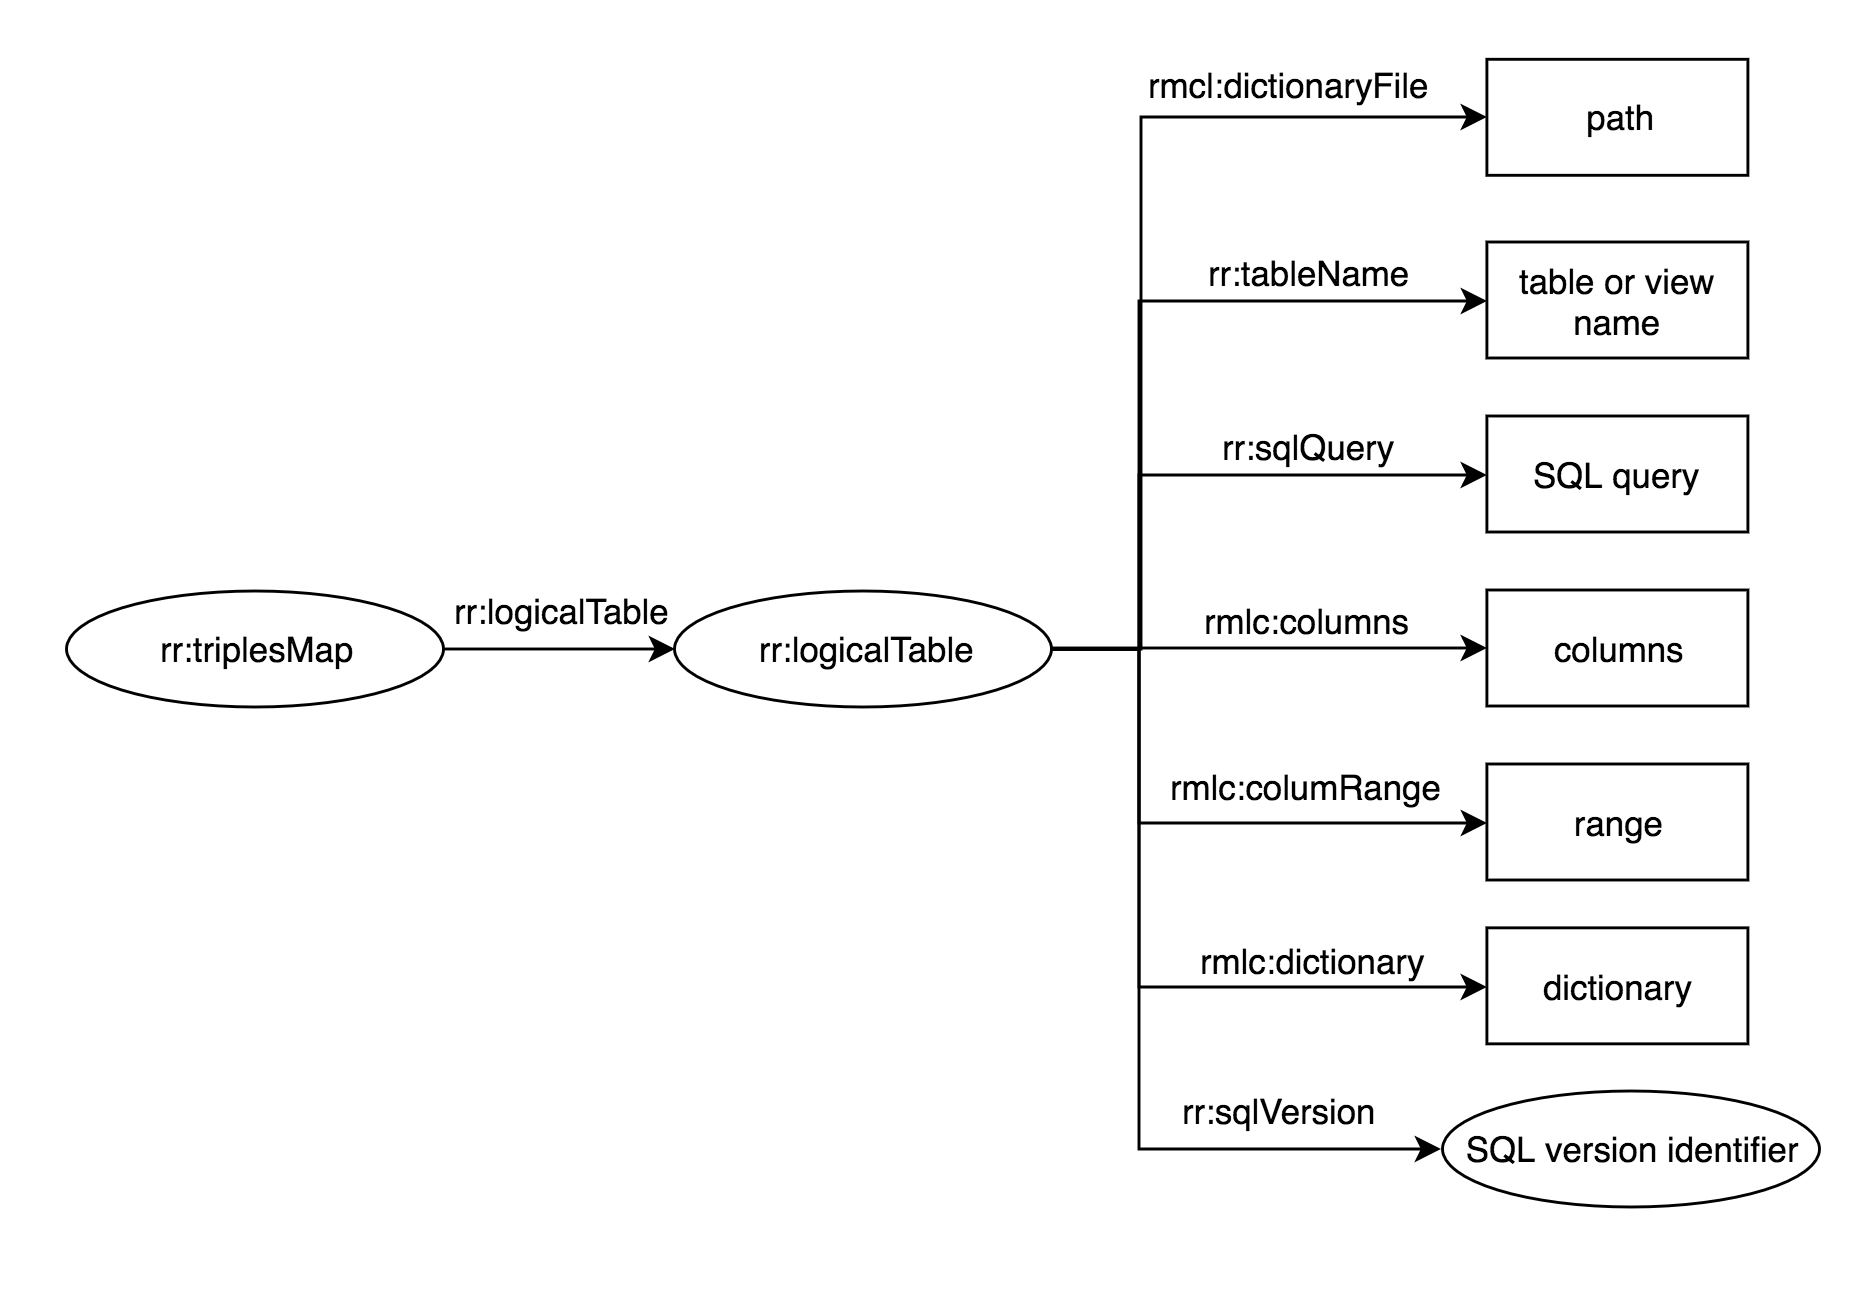
\includegraphics[width=1.0\linewidth]{figures/rmlc-iterator.png}
  \caption{R2RML extension for statistics tabular data}
  \label{fig:rmlc}
\end{figure}
\lstset{upquote=true}
\begin{lstlisting}[float,caption=Columns and dictionary properties in R2RML-Iterator,frame=tlrb,label={list:columns}, columns=fullflexible]
rr:logicalTable [
    rr:tableName "\"2016-P21\"";
    rmlc:columns ("Jan" "Oct" "Dec");
    rmlc:dictionary ("Jan:January" "Oct:October","Dec:December");
];
\end{lstlisting}

\begin{lstlisting}[float,caption=Iterator variables in the extension,frame=tlrb,label={list:iterator}, columns=fullflexible]
<TriplesMap2016{$column}>

rr:subjectMap [
    a rr:Subject;
    rr:template "http://ex.org/2016{$column}";
    rr:termType rr:IRI;
    rr:class qb:Observation;
];
rr:predicateObjectMap[
	rr:predicate sltsv:month;
    rr:objectMap [
    	rr:termType rr:IRI;
        rr:constant "http://reference.data.gov.uk/def/intervals/{$alias}";
    ];
];
rr:predicateObjectMap[
    rr:predicate sltsv:numberOfArrivals;
    rr:objectMap [
        rr:termType rr:Literal;
        rr:column {$alias};
        rr:datatype xsd:integer;
    ];
];
\end{lstlisting}
\lstset{upquote=false}



\begin{table}[t]
\centering
\caption{Excerpt of statistics data to be transformed follow RDF Data Cube data model}
\label{tab:example-stadistics}
\resizebox{\textwidth}{!}{%
\begin{tabular}{l|c|c|c|c|c|c|c|c|c|c|c|c|c}
\hline
\textbf{CountryofResidence} & \textbf{TOTAL} & \textbf{Jan} & \textbf{Feb} & \textbf{Mar} & \textbf{Apr} & \textbf{May} & \textbf{Jun} & \textbf{Jul} & \textbf{Aug} & \textbf{Sep} & \textbf{Oct} & \textbf{Nov} & \textbf{Dec} \\ \hline
Canada      & 44122  & 4016  & 3521  & 3900  & 2962  & 3319 & 4111 & 5330  & 5044  & 2527  & 2345  & 2447  & 4600  \\ \hline
USA         & 54254  & 5144  & 4851  & 5265  & 3408  & 3538 & 3917 & 4919  & 4061  & 3276  & 3432  & 4223  & 8220  \\ \hline
Austria     & 16995  & 2463  & 2917  & 1949  & 774   & 596  & 395  & 1456  & 1232  & 649   & 1063  & 1422  & 2079  \\ \hline
Belgium     & 14387  & 1285  & 1552  & 1639  & 675   & 377  & 586  & 2705  & 1511  & 1180  & 688   & 839   & 1350  \\ \hline
Denmark     & 18097  & 2892  & 3029  & 2216  & 679   & 490  & 1096 & 2632  & 783   & 502   & 921   & 896   & 1961  \\ \hline
France      & 96440  & 9878  & 14602 & 11175 & 7518  & 3281 & 3659 & 10949 & 10805 & 5008  & 5849  & 5845  & 7871  \\ \hline
Netherlands & 41373  & 3194  & 3555  & 2442  & 2496  & 1458 & 1711 & 9755  & 4726  & 2915  & 2272  & 2941  & 3908  \\ \hline
Italy       & 29791  & 4131  & 3607  & 2683  & 1455  & 1010 & 1390 & 2418  & 4517  & 1392  & 1274  & 1803  & 4111  \\ \hline
Norway      & 12790  & 1164  & 1336  & 1318  & 496   & 374  & 1825 & 2260  & 644   & 504   & 808   & 877   & 1184  \\ \hline
Spain       & 19425  & 984   & 1054  & 1587  & 856   & 719  & 735  & 2371  & 3888  & 1846  & 1758  & 1691  & 1936  \\ \hline
Sweden      & 21589  & 3715  & 3277  & 2339  & 771   & 416  & 859  & 937   & 498   & 466   & 1305  & 1943  & 5063  \\ \hline
Switzerland & 26282  & 2483  & 2580  & 2122  & 1870  & 966  & 1208 & 5540  & 1672  & 1432  & 2103  & 1695  & 2611  \\ \hline
UK          & 188159 & 16253 & 19194 & 21430 & 12006 & 8412 & 9406 & 23948 & 20475 & 12288 & 10964 & 13337 & 20446 \\ \hline
\end{tabular}%
}
\end{table}

Listing \ref{list:columns} depicts an example of the usage of the \texttt{rmlc:columns} property, in which the subset of the CSV columns (see Table \ref{tab:example-stadistics}) to be used in the transformation process is specified. This property is defined using a LogicalTable object. We use the \texttt{rmlc:dictionary} (or its corresponding \texttt{rmlc:dictionaryFile}) property to establish a correlation between a column and its alias, that is useful in some parts of the mappings. These properties are based on JSON syntax for easing their creation to the mapping editors.

During the mapping translation process, the variables are replaced with the name of each column or its alias, as defined in the LogicalTable object. The resulting R2RML mapping contains as many TriplesMap objects as the number of columns specified in the R2RML-iterator properties. In this example, the identifier of each TriplesMap, the URI of the subjects and the object of the \texttt{sltsv:numberOfArrivals} predicates, include the variables so they will be replaced with the name of a column or its alias. The R2RML mapping will contain three TriplesMap objects, one for each defined column. All the iterator variables can be specified anywhere in the mapping, as shown in Listing \ref{list:iterator}, using the \{\$column\} or \{\$alias\} syntax.

In order to ensure that the iterator proposal aligns with R2RML, we have developed a mapping translator that converts its mapping document with an iterator variable to a R2RML mapping with multiple TriplesMap objects. In this way, we reduce the size of the R2RML mapping document, minimizing the time of the mapping creation and supporting an easier maintenance. Besides, as it is aligned to R2RML, any R2RML available processor is able to deal with our approach. 

\subsection{R2RML iterator: Use Cases}
In this section we describe our experiment of transforming two statistics datasets from two different domains and agencies: a tourism statistics dataset from the Sri Lanka Tourism Development Authority (SLTDA) and a immigration statistics from the EuroStat. For each dataset, we use both R2RML and R2RML-Iterator mappings with Morph-RDB to generate virtual SKGs and evaluate three SPARQL queries for each one.

\subsubsection{Case 1: Statistics from the Sri Lanka Tourism Development Authority}
\noindent\paragraph{Dataset and Queries.}
The Sri Lanka Tourism Development Authority performs data collection and market research about tourism in Sri Lanka and publishes comprehensive statistics as PDF files\footnote{\url{http://www.sltda.lk/statistics}}. We use tabula-java\footnote{\url{https://github.com/tabulapdf/tabula-java}} to extract these statistics as CSV files and make them available online. For example, the CSV file that contains the number of passengers grouped by countries (y-axis) and the arrival months (x-axis) in 2016.

Our intention is to transform that CSV file into a virtual SKG. Because this SKG is not materialized, there is no need to store it in a dedicated triple store. Any R2RML engine with query translation support will be able to answer SPARQL queries posed to the dataset. For example, consider the following three queries:
\begin{itemize}
\item Q1: Retrieve observations of the number of incoming tourist originated from Spain in 2016.
\item Q2: Retrieve observation of the number of incoming tourists in May 2016.
\item Q3: Can be seen as the combination between Q1 and Q2, i.e., retrieve observations of the number of incoming tourists from Spain in May 2016. 
\end{itemize}

\noindent\paragraph{Mappings.}
The R2RML mapping document generated using the naive approach described in the previous section contains 12 TriplesMaps and around 700 lines. Each TriplesMap describes the transformation rules of the number of arriving passengers every month of the year. Except for those PredicateObjectMap properties corresponding to the name the CSV columns, all TripleMaps have identical values. 

On the contrary, the corresponding proposal mappings, either with \texttt{rmlc:column} property or with \texttt{rmlc:range} property have only 74 lines in total with 1 TriplesMap and 5 PredicateObject mappings. The Table \ref{table:compare1} summarizes the characteristics of the mappings.

\begin{table}[tbp]
\caption[R2RML vs R2RML-iterator in Sri Lanka dataset]{Comparison between R2RML and R2RML-iterator mappings used in the Sri Lanka Tourism dataset example.}
\label{table:compare1}
\begin{tabular}{c|c|c}
\hline
\textbf{Features} & \textbf{R2RML}   & \textbf{R2RML-iterator}  \\ \hline
Total Lines   & $\sim$700 & 74 \\ 
\#TriplesMaps / \#SubjectMaps     & 12                & 1           \\
\#PredicateObjectMaps  & 60              & 5            \\ \hline
\end{tabular}
\end{table}

\subsubsection{Case 2: EuroStat - Immigration Statistics}
\noindent\paragraph{Dataset and Queries.} Eurostat\footnote{\url{http://ec.europa.eu/eurostat}} publishes the statistics office of the European Union. Its main responsibility is to provide statistics information about European Union such as economy, finance, population, industry, etc. In this example, we consider a dataset containing the number of immigrants that have arrived in European countries available online\footnote{\url{http://ec.europa.eu/eurostat/product?code=tps00176&mode=view}}. We downloaded the aforementioned dataset as a CSV file containing the number of immigrants grouped by countries (x-asis) and years (y-axis). We have created three SPARQL queries, similar to the ones in the previous example:

\begin{itemize}
\item Q1: Retrieve the number of immigrants arriving in Spain.
\item Q2: Retrieve the number of immigrants arriving in any of European Countries in the year of 2015.
\item Q3: Retrieve the number of immigrants arriving in Spain in the year of 2015.
\end{itemize}

\noindent\paragraph{Mappings.}
Generating the naive mapping described in the first approach is not feasible in this case, as there is a need to generate a TriplesMap for each column that represents a country and the dataset contains more than 40 columns. Instead, we generate two R2RML-iterator mapping documents,one with \texttt{rmlc:columns} property and the other with \texttt{rmlc:range} property. Then we use the our mapping translator engine to generate the naive version of R2RML.

Our proposals mapping document (either version) contains only 1 TriplesMap and 4 PredicateObjectMap mappings, totalling less than 70 lines. On the contrary, the generated R2RML mapping document has more than 40 TriplesMap, more than 170 PredicateObjectMap mappings, totalling more than 2800 lines. The Table \ref{table:compare2} summarizes the characteristics of the mappings.
\begin{table}[tbp]
\caption[R2RML vs R2RML-iterator in Eurostat dataset]{Comparison between R2RML and R2RML-iterator mappings used in the Eurostat Immigration dataset example.}
\label{table:compare2}
\begin{tabular}{c|c|c}
\hline
\textbf{Features} & \textbf{R2RML}   & \textbf{R2RML-iterator}  \\ \hline
Total Lines   & $>$2800 & $<$70 \\ 
\#TriplesMaps / \#SubjectMaps     & $>$40                & 1           \\
\#PredicateObjectMaps  & $>$170              & 4            \\ \hline
\end{tabular}
\end{table}


\section{Conclusions}

In this chapter, we have discussed the concept of mapping translation, which had not been addressed before in the literature. We have shown how this concept has been actually implemented in some approaches addressing the readability and maintenance of mappings, the generation of programming code to provide access to heterogeneous data sources, or the enrichment of original data sources, among others. Additional, the mapping translation concept is the main idea behind the optimizations proposed in this thesis and described in detail in Chapter \ref{chapter:virtual} and Chapter \ref{chapter:construction}.

We think that this concept needs to be explored further, and this would allow a new range of KGC approaches that may be part of a new generation, as claimed in the title of the chapter. The KGC community\footnote{\url{https://www.w3.org/community/kg-construct/}} should see this variety of mapping languages not only as challenges (e.g., interoperability) but also, and mainly, as an opportunity for further research and development in this area, to address the need to cover more types of data sources while taking advantage of all the work that has been done in advanced aspects like query translation. Providing mapping translator services across mapping languages would bring further benefits and increase the availability of ontology-based data for its exploitation by search engines and query answering systems at Web scale.

\chapter{Systematic Evaluation for Knowledge Graph Construction Engines}
\label{chapter:evaluation}
In this chapter, we present the contributions related with the evaluation of knowledge graph construction systems. On the one hand, the evaluation is relevant for application developers who may need to understand the strengths and weaknesses of existing knowledge graph construction tools. On the other hand, tool developers may want to know whether their engines cover the requirements of real use-case scenarios. In general, it is necessary to have an overview of state of the art engines that are tailored to different source formats, accepting as input mappings that are represented in a variety of declarative languages. 

 Section \ref{chapter5:sec-rml} describes a preliminary set of test cases for testing the conformance of RML mapping language over its available processors, Section \ref{chapter5:sec-param} describes and analyzes the impact of several parameters for the evaluation of materialized KGC engines together with the definition of a set of representative testbeds and their evaluation over two compliant RML engines. Finally, Section \ref{chapter5:sec-bench} presents a virtual knowledge graph construction benchmark over the transport domain. Additionally to the benchmark proposal, an experimental evaluation is performed over four different engines from the state of the art. The three contributions of this chapter define a systematic and comprehensive framework that allow the identification of strengths and weakness of KGC engines.



\section{Conformance Test Cases for the RDF Mapping Language (RML)}

Knowledge graphs are often generated based on rules that apply semantic annotations to certain data. For example, the DBpedia knowledge graph is generated by applying classes and predicates of the DBpedia ontology to Wikipedia \citep{lehmann_2015_swj}. Software tools execute these rules and generate corresponding RDF triples and quads \citep{RDF},
which materialize knowledge graphs. In the past, custom scripts prevailed, but lately rule-driven tools emerged. Such tools distinguish the rules that define how RDF terms and triples are generated from the tool that executes them. R2RML \citep{R2RML} is the W3C recommended language to define such rules for generating knowledge graphs from data in relational databases (RDBs). An R2RML processor is a system that, given a set of R2RML rules and a relational database, generates an output RDF dataset. Examples of R2RML processors are, e.g., Ultrawrap \citep{sequeda_2013_jws}, Morph-RDB \citep{priyatna2014formalisation}, Ontop \citep{calvanese2017ontop}, and XSPARQL \citep{bischof_2012_jds}. A subset of them was included in the RDB2RDF Implementation Report \citep{R2RML} to determine their conformance to the R2RML specification \footnote{Some of those available in the report are no longer actively maintained and used}, i.e., the correct knowledge graph is generated for a set of rules
and certain relational database.

%Need: Why something needed to be done at all
Extensions and adaptations were applied to R2RML to account for other types of data sources, given that R2RML is focused on relational databases only,
such as RML~\citep{dimou2014rml}, XSPARQL~\citep{bischof_2012_jds}, xR2RML~\citep{michel2015translation}, KR2RML~\citep{slepicka2015kr2rml}, and D2RML~\citep{chortaras2018d2rml}. RML provides an extension of R2RML to support heterogeneous data sources, including different formats, e.g., CSV, XML, JSON, and access interfaces, e.g., files and Web APIs. Similarly, RML processors emerged that execute RML rules, such as the RMLMapper\footnote{RMLMapper, \url{https://github.com/RMLio/rmlmapper-java}}, CARML\footnote{CARML, \url{https://github.com/carml/carml}}, GeoTriples\footnote{GeoTriples, \url{https://github.com/LinkedEOData/GeoTriples}}, and Ontario\footnote{Ontario,\url{https://github.com/WDAqua/Ontario}}.
Unlike R2RML, there are no test cases available to determine the conformance of the processors to the RML specification. As a result, the processors are either not tested or only tested with custom test cases, which do not necessarily assess every aspect of the specification. Consequently, no implementation report is available that allows comparing the different processors that generate knowledge graphs from heterogeneous data sources
based on the conformance to the specification. This way it is hard to determine the most suitable processor for a certain use case.

%Task: What was undertaken to address the need
%Object: What the present document does or covers
In this work, (i) we focused on RML and introduce an initial set of RML test cases, which contains 297 test cases based on the existing R2RML test cases. However, instead of only considering relational databases as data sources, as it occurs for the R2RML test cases, we also consider data in CSV, XML, and JSON format. Furthermore, (ii) we tested the conformance of the RMLMapper and CARML: every test case is executed by each processor and we noted if the generated knowledge graph matches the expected one. The corresponding implementation report is available at \url{http://rml.io/implementation-report}. This allows to determine which processor is the most suitable for a certain use case. For example, do users want a processor that supports the complete specification, or do they prefer a processor that does not support certain aspects of the specification,
but executes the rules faster?

%Findings: What the work done yielded or revealed
The test cases results shows that the RMLMapper passes all test cases regarding CSV, XML, and JSON format, and most test cases for RDBs, but fails the test cases for automatic datatyping of literals. CARML passes most test cases regarding CSV, XML, and JSON format, except of the test cases that deal, for example, with multiple RDF terms generation. Users can now determine how conformant the different processors are to the RML specification and use this conformance to determine the most suitable processor for their use cases.

\subsection{RML Test Cases}
\begin{figure}[!th]
\centering
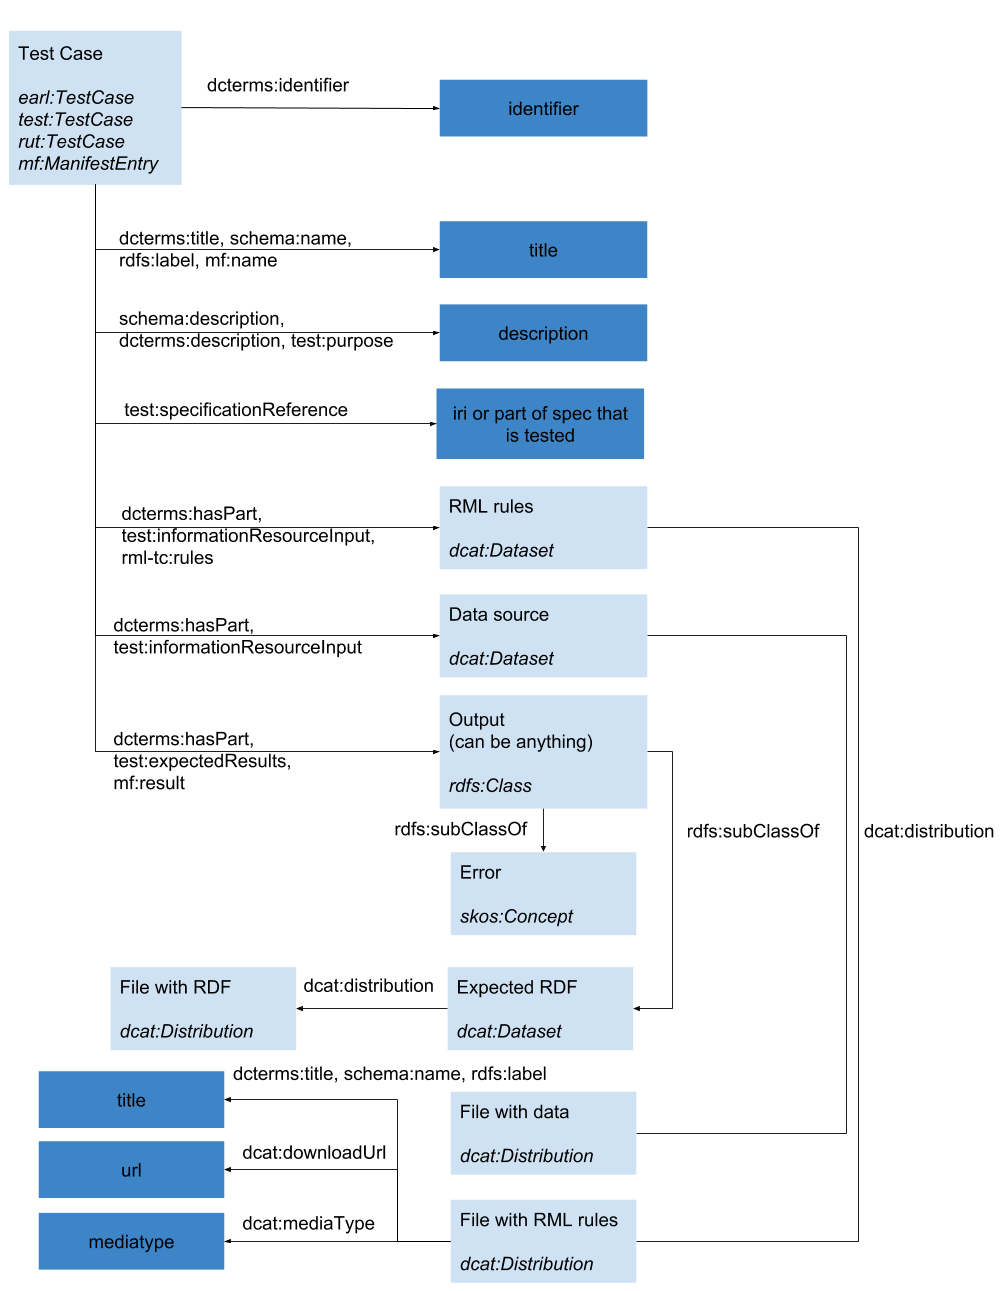
\includegraphics[width=0.9\textwidth]{figures/rml_test_case_model.png}
\caption{Data model of the RML test cases}
\label{fig:datamodel}
\end{figure}

In this section, we propose test cases to determine the conformance of RML processors to the RML specification. The proposed test cases are based on the R2RML test cases, but they take into account different heterogeneous data sources and the corresponding differences in RML. Our preliminary set of test cases includes (i)~adjusted R2RML test cases for relational databases (including MySQL\footnote{\url{https://www.mysql.com/}}, PostgreSQL\footnote{\url{https://www.postgresql.org/}}, and SQL Server\footnote{\url{https://www.microsoft.com/en-us/sql-server/}}) and (ii)~new test cases for files in the CSV, XML (with XPath as the reference formulation), and JSON format (with JSONPath as the reference formulation). The test cases are described at \url{http://rml.io/test-cases/} and the corresponding files are available at \url{https://github.com/rmlio/rml-test-cases}. In Section \ref{sec:datamodel}, we describe the data model that is used to represent the test cases. In Section \ref{sec:test-case-files}, we elaborate on the different files making up a test case. In Section \ref{sec:diff-r2rml-test-cases}, we discuss the differences between the R2RML and RML test cases.

\subsubsection{Data model}

We describe the test cases semantically to increase their reusability and sharability. To this end, we created a semantic data model\footnote{\url{http://rml.io/test-cases/\#datamodel}}, with as main entity the test case (see Figure \ref{fig:datamodel}). For each test case, the following details are described: unique identifier, title, description, relevant aspect of the RML specification, data sources (optional), expected knowledge graph or error, and RML rules.

To provide the corresponding semantic descriptions, the model uses mostly the Evaluation and Report Language (EARL) 1.0 Schema\footnote{\url{https://www.w3.org/TR/EARL10/}, with prefix \texttt{earl}}, the Test case manifest vocabulary\footnote{\url{http://www.w3.org/2001/sw/DataAccess/tests/test-manifest\#}, with prefix \texttt{mf}}, the Test Metadata vocabulary\footnote{\url{https://www.w3.org/2006/03/test-description\#}, with prefix \texttt{test}}, and the Data Catalog Vocabulary\footnote{\url{https://www.w3.org/TR/vocab-dcat/}, with prefix \texttt{dcat}}. A test case is annotated with the classes \verb|earl:TestCase|, \verb|test:TestCase|, and \verb|mf:ManifestEntry|. The identifier, title, description, and the specific aspect of the RML specification that is being tested are added as datatype properties. The files that are provided as input to the tools are linked to the test cases via \verb|test:informationResourceInput| and \verb|dcterms:hasPart|. The file with the RML rules is also linked via \verb|rml-tc:rules|\footnote{\url{http://rml.io/ns/test-cases}, with prefix \texttt{rml-tc}}. The objects of these properties are of the class \verb|dcat:Dataset|,which in turn link to a \verb|dcat:Distribution| that includes a link to a file. The expected output, whether that is a knowledge graph or an error, is linked via \verb|test:expectedResults|, \verb|mf:result|, and \verb|dcterms:hasPart|. In the case of a knowledge graph, the object of these properties is a \verb|dcat:Dataset|, linked to a \verb|dcat:Distribution|, to describe the file containing the graph. In the case of an error, we link to the expected error.

\subsubsection{Test case files}

Each test case consists of a set of files that contain the input data sources, the RML rules, and the expected RDF output. In practice, the files are organised as follows: all files for a single test case are contained in a single folder. There are three types of files for each test case:

\begin{itemize}
  \item 0 or more \textbf{data source files} for CSV (with extension .csv), XML (with extension .xml), and SON (with extension .json), or 
  1 file with SQL statements to create the necessary tables for relational databases (called \verb|resource.sql|);
  \item 1 \textbf{file with the RML rules} (in Turtle format, called \verb|mapping.ttl|); and
  \item 0 or 1 \textbf{file with the expected RDF} (in N-Quads format, called \verb|output.nq|).
\end{itemize}

Distinct test cases assess different behaviours of the processors. Certain test cases assess the behaviour of the tools when (i)~the required data sources are not available, and others when (ii)~an error occurs and no output is generated. In the former, no data sources files or SQL statements are provided. In the latter, no file with the expected RDF is provided. The test cases are independent of how the processors materialize the knowledge graph: a data dump, as done by the RMLMapper, or on the fly, as done by Ontario~\citep{endris2019ontario}.

\subsubsection{Differences with R2RML test cases}
For most R2RML test cases, we created an RML variant for CSV, XML, JSON, MySQL, PostgreSQL, and SQL Server, leading to 6 RML test cases per R2RML test case. For R2RML test cases that focus on specific features of SQL queries, we only created 3 RML test cases, i.e., for MySQL, PostgreSQL, and SQL Server.

For test cases with CSV, XML, and JSON files as data sources, we created the corresponding files with the data based on the tables of the relational databases. For CSV, we used the table created by the SQL statements of the R2RML test case and stored it as a CSV file. For XML, the name of the table was used for the root of the XML document and every row of the table was used to create an XML element. Within this element, elements were created for each column and their values are the values of the corresponding columns in the table. For JSON, we followed a similar approach as XML. The file contains a JSON object at the root with the name of the table as the only attribute. This attribute has as value an array, where each element of the array corresponds with a row in the table. For each row, attributes were created for each column and their values are the values of the corresponding columns in the table.

\paragraph{Data errors.}
2 of the R2RML test cases expect a data error to happen, e.g., when the subject IRI of an entity cannot be generated. In this case, an error is thrown and no knowledge graph is generated. With RML for entities where no subject IRI can be generated there is also no output generated, but, in contrast to R2RML, for the other entities the corresponding output is still generated. Therefore, for the corresponding RML test cases the processors can still throw an error, but the generation of the knowledge graph must not be halted.

\paragraph{Inverse expressions.}
3 of the R2RML test cases are designed to test the use of inverse expressions\footnote{\url{https://www.w3.org/TR/r2rml/\#inverse}}. However, inverse expressions are only used to optimize the knowledge graph generation and no differences are observed in the generated knowledge graph. Thus, whether inverse expressions are used by a processor or not cannot be verified by such test cases. Thus, we do not include them for RML.

\paragraph{SQL-specific features.}
18 of the R2RML test cases focus on specific features of SQL queries, e.g., a duplicate column name in a SELECT query. As there are no corresponding RML test cases for CSV files, XML files with XPath, and JSON files with JSONPath, we only provide 54 corresponding test cases for MySQL, PostgreSQL, and SQL Server.

\paragraph{Null values.}
1 of the R2RML test cases tests null values in the rows. However, a corresponding RML test case cannot be provided for the CSV and XML format, because both formats do not support null values.

\paragraph{Spaces in columns.}
1 of the R2RML test cases is designed to test the behaviour when dealing with spaces in the columns of the SQL tables. However, a corresponding RML test case cannot be provided for the XML format, because it does not allow spaces in names.
\\
\\
In total, we have 297 test cases: 39 for CSV, 38 for XML, 41 for JSON, and 180 for relational databases. Of these 297, 255 test cases expect an knowledge graph to be generated, while 36 expect an error that halts the generation.

\subsection{Conformance of RML Parsers}

In this section, we describe the executing of the test cases and their results for two RML processors: the RMLMapper and CARML. 
We detail on
(i) the method for running the test cases and obtaining the results, which are annotated semantically, and 
(ii) the implementation report similar as proposed for R2RML\footnote{\url{https://www.w3.org/TR/rdb2rdf-implementations/}}.  After this, we present the results of the RMLMapper and CARML. 

\subsubsection{Method}
We define a method to run the RML test cases over RML processors and generate the corresponding results. The main goal is to facilitate the testing process and provide a general solution for running the test cases over other RML processors that can be developed in the future. The method consists of two main steps: (i) assessing if a processor passes every test case and (ii) annotating the obtained results as RDF using the EARL Schema through a set of YARRRML rules~\citep{Heyvaert2018Declarative}.

We implemented a Java-based tool for checking the conformance of the test cases over different RML processors. At this moment, it is able to evaluate the test cases for JSON, CSV and XML formats. We relied on the test framework of each processor to execute the RDB test cases. If a new processor wants to be added to test its conformance, the framework only needs to have access to the corresponding output of each test-case. Then it checks, using the same method for all processors, if the output is the same as the correct one, if an error that is expected has really thrown, etc. The code is available online\footnote{\url{https://github.com/RMLio/rml-implementation-report}} together with a Web page showing the results of all tested tools\footnote{\url{http://rml.io/implementation-report}}. It generates as output two CSV files with the results and the metadata needed to generate the corresponding RDF.

%For obtaining the RDF from the results 
The results are semantically annotated, as the test cases, using the EARL Schema. Each test case evaluated by a tool is annotated as an \texttt{earl:Assertion} with the properties: \texttt{earl:subject} with the URI of the tool, \texttt{earl:assertedBy} with the identifier of who performed the evaluation, \texttt{earl:test} with the URI of the test and \texttt{earl:result} with the result of the test-case. 

Three types of results are possible: ``passed'', ``failed'', and ``inapplicable''. \textbf{Passed} (\texttt{earl:passed}) is used either when the actual output matches the expected output when no error is expected, or when the tool throws an error when an error is expected. \textbf{Failed} (\texttt{earl:failed}) is used either when the actual output does not match the expected output if no error is expected, the processor returns an error trying to execute a test or the tool does not throw error if an error is expected. \textbf{Inapplicable} (\texttt{earl:inapplicable}) is used when the tool clearly states that specific features used in a test case are not supported. 
%Together with this value, 
The results also provide its type (\texttt{earl:TestResult}) and its mode (\texttt{earl:automatic} for all these cases). 
We created a set of YARRRML rules to generate these annotations following the EARL Schema that, using the outputs of the test cases.
%generate the corresponding RDF.

\subsubsection{Results}
We perform the test-cases over two processors: RMLMapper and CARML. In Table \ref{tab:rmlmapper} we show the results for the RMLMapper processor. It passes all CSV, JSON and XML test cases, but fails in the same 5 test cases for the RDBs. The failures are related to the automatic datatyping of literal for RDBs specified by R2RML\footnote{\url{https://www.w3.org/TR/r2rml/\#dfn-natural-rdf-literal}}. RMLMapper expects to pass the failed test-cases in next versions of the processor. The effort prediction to pass these test-cases is not very much since the failures depend on the general processor, not on the used RDBMS. Once they have been solved for one RDBMS they will automatically pass over the rest.

In Table \ref{tab:carml} we show the results for the CARML processor. It partially passes the CSV, JSON and XML test cases, but it does not provide support for any of the RDBs test cases. The failures are related to the unsupported for multiple Subject Maps, multiple Predicate Maps, and Named Graphs. The developers of the tool declare that CARML will support these features in next versions of the processor. However, at the moment of writing, we do not have any information about if CARML will provide support for RDBs.

Finally, we can declare that testing a RML processor with the defined cases and analysing the obtained results offers a general view of the current status of it. These results also give useful information to the tool developers on knowing where they should put their effort to improve the conformance of the processor.

\begin{table}[]
\centering 
\caption[RML test-cases results for RMLMapper]{Results of the RMLMapper}
\label{tab:rmlmapper}
\renewcommand{\arraystretch}{1.5}
\begin{tabular}{c|c|c|c|c|c|c|c}

RMLMapper                 & \textbf{CSV} & \textbf{XML} & \textbf{JSON} & \textbf{MySQL} & \textbf{PostgreSQL} & \textbf{SQL Server} & \textbf{Total} \\ \hline
\textbf{passed}       & 39           & 41           & 38            & 55              & 55               & 55                   & 283             \\ \hline
\textbf{failed}       & 0           & 0           & 0            & 5              & 5                   & 5                   & 15             \\ \hline
\textbf{inapplicable} & 0            & 0             & 0             & 0             & 0                  & 0                  & 0            \\ 
\end{tabular}
\end{table}


\begin{table}[]
\centering
\caption{RML test-cases results for CARML}
\label{tab:carml}
\renewcommand{\arraystretch}{1.5}
\begin{tabular}{c|c|c|c|c|c|c|c}

CARML                 & \textbf{CSV} & \textbf{XML} & \textbf{JSON} & \textbf{MySQL} & \textbf{PostgreSQL} & \textbf{SQL Server} & \textbf{Total} \\ \hline
\textbf{passed}       & 29           & 28           & 28            & 0              & 0                   & 0                   & 85             \\ \hline
\textbf{failed}       & 10           & 10           & 13            & 0              & 0                   & 0                   & 33             \\ \hline
\textbf{inapplicable} & 0            & 0             & 0             & 60             & 60                  & 60                  & 180            \\ 
\end{tabular}
\end{table}

\section{Parameters that Affect the Construction of a Knowledge Graph}
\label{chapter5:sec-param}
In this section, we study the process of knowledge graph construction and analyze various variables and configurations that can impact on the performance of materialization techniques. The relevant parameters studied in this work include selectivity of the joins between mapping rules, types of relations, and percentage of duplicates. We also present diverse examples that evidence the heterogeneous behavior that each engine may exhibit whenever small changes are conducted to the variables and the configurations of a testbed.  

We devise a set of parameters involved in a knowledge graph construction process and we empirically show how they can impact on the behavior of two existing engines: RMLMapper\footnote{\url{https://github.com/RMLio/rmlmapper-java}} and SDM-RDFizer\footnote{\url{https://github.com/SDM-TIB/SDM-RDFizer}}; these engines are mostly fully compliant with the RML specification according to our results in the Section \ref{chapter5:sec-rml}. We develop a synthetic data generator for the generation of (semi)-structured data and RML mapping rules, that consider the identified set of parameters. The results of our empirical study provide evidence of the importance of the proposed set of variables and configurations during the evaluation of these tools. The testbeds used to conduct this evaluation are available
online\footnote{\url{https://github.com/SDM-TIB/KGC-Param-Eval}}.

Our main contribution includes the definition of various dimensions and set of variables to be considered during the creation of testbeds or to be measured while the evaluation of knowledge graph construction tools. Another contribution represents the empirical evaluation of the effects that the variables and configurations have on the tasks of knowledge graph construction. Furthermore, the results of the experimental study contribute to the understanding of the pros and cons of the studied engines, and the directions that need to be followed in order to devise tools able to scale up to real-world scenarios.  

\subsection{Motivation Example}

We motivate our work by analyzing different scenarios where the performance of RMLMapper and SDM-RDFizer may be affected by changing the configuration of the testbeds utilized for empirically evaluating these engines. We aim at remarking the importance of taking into account different parameters during the definition of a testbed. We first describe a scenario where na\"ive parameters (size and format) leads to wrong decisions during the comparing of SDM-RDFizer and RMLMapper. The testbeds include a data source with one thousand rows, different number of predicate-object (POM) in RML triple maps, and diverse configurations of selectivity of triple map joins.

%\begin{figure}[t!]
%	\centering
%	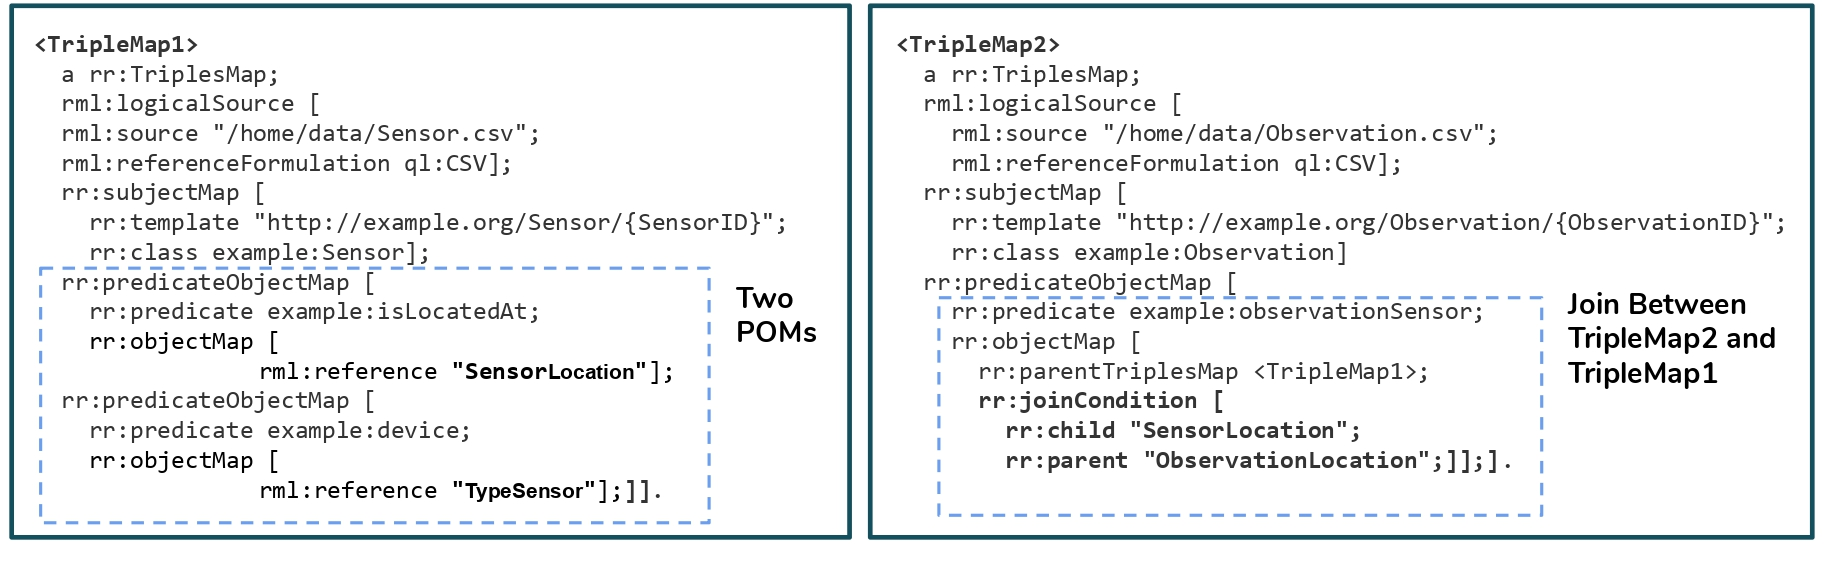
\includegraphics[width=\columnwidth]{figures/TripleMap.jpg}
%	\caption[RML Mapping example]{{\bf Motivating Example.} RML triple maps to transform two CSV files into RDF. TripleMap1 is composed of two predicate-object, i.e., Two POM. TripleMap2 has a join to TripleMap1; Observation.csv (outer relation) is joined to  Sensor.csv (inner relation) and the result, SensorID, is used as an object value.}
%	\label{fig:mappingRule}
%\end{figure}

%RML expresses mappings to transform sources represented in (semi)-structured format, e.g. CSV or XML, into RDF. Each mapping rule in RML, named RML triple map, is represented in RDF and consists of the following parts \citep{dimou2014rml}:
%\begin{itemize}
%    \item A \emph{Logical Source} that refers to a data source from where data is collected.
%    \item A \emph{Subject Map} that defines the subject of the generated RDF triples. 
%    \item \emph{Predicate-Object Maps} (POM) that expresses the predicate and the object the RDF triple to be generated; a triple map can comprise several POMs.
%\item
%A \emph{Referencing Object Map}, that indicates the reference or join condition to another triple map; the subject URL is the referenced triple map corresponds to the result of the evaluation of the join. 
%\end{itemize}
%\autoref{fig:mappingRule} illustrates two RML triple maps. \texttt{TripleMap1} is composed of two predicate-object maps, i.e. it is a Two POM mapping rule. \texttt{TripleMap2} has a referencing object map that joins the records of file Observation.csv with the records of the file Sensor.csv on the attributes \texttt{SensorLocation} and \texttt{ObservationLocation}. The result of executing the join between the two RML triple maps is the identifier of the sensor that collected the observation; this value is used as the object value of the predicate \texttt{observationSensor}.
%\subsubsection{Impact of Number of Predicates and Objects in Mapping Rules}
In this example, we execute a testbed where three different configurations of an RML mapping rule: Two-POM, Five-POM, and Ten-POM, i.e. they correspond to three mapping rules with two, five, and ten Predicate-Object Maps, respectively. 
Both engines exhibit a similar behavior while the number of predicate-object maps varies from two to five POMs, as shown in Table~\ref{tab:trivial}. However, when more complex mapping rules with more POMs are considered, the behavior of the SDM-RDFizer and RMLMapper is not impacted equally. Moreover, the results suggest that RMLMapper execution time increases with the number of POMs, while the SDM-RDFizer seems to be slightly affected. 
\begin{table}[ht!]
\centering
\caption[Impact of number of POMs on KGC engines]{\textbf{Impact of Number of Predicate-Object Maps.} Various predicate object maps (POM) specified in the mapping rules. The behavior of the two engines is similar when the mapping rules are simple (less than 5 POM) but it is different when more complex mappings are running (10 POM); time in seconds.
}
\label{tab:trivial}
\begin{tabular}{|l|c|c|}
\hline
\multicolumn{1}{|c|}{\multirow{2}{*}{\textbf{Engine}}} & \textbf{\begin{tabular}[c]{@{}c@{}}Execution \\ time (secs.)\end{tabular}} & \multicolumn{1}{l|}{\textbf{Number of results}} \\ \cline{2-3} 
\multicolumn{1}{|c|}{} & \multicolumn{2}{c|}{\textbf{Two POM}} \\ \hline
\multicolumn{1}{|c|}{\textbf{RMLMapper}} & 0.92  & 2,000 \\ \hline
\multicolumn{1}{|c|}{\textbf{SDM-RDFizer}} & 1.72 & 2,000 \\ \hline
\multicolumn{1}{|c|}{\textbf{}} & \multicolumn{2}{c|}{\textbf{Five POM}} \\ \hline
\textbf{RMLMapper} & 1.84 & 5,000 \\ \hline
\textbf{SDM-RDFizer} & 1.85 & 5,000 \\ \hline
 & \multicolumn{2}{c|}{\textbf{Ten POM}} \\ \hline
\textbf{RMLMapper} & 3.36 & 10,000 \\ \hline
\textbf{SDM-RDFizer} & 1.98 & 10,000 \\ \hline
\end{tabular}
\end{table}
%\subsubsection{Impact of Join Selectivity}
We now consider another parameter, the join selectivity, i.e. the cardinality of matching values from outer to the inner table (relation), in a referencing object map between two RML mapping rules. The join selectivity varies from 
\textbf{High Selectivity}, \textbf{Medium Selectivity}, and \textbf{Low Selectivity}, and Table~\ref{tab:joinSelectivity} reports on the results of RMLMapper and  SDM-RDFizer. First, it can be observed that the RMLMapper execution time increases by around $8$ seconds, while the SDM-RDFizer behavior is not equally affected by the selectivity of the join condition. As can be seen in Table~\ref{tab:joinSelectivity}, the SDM-RDFizer execution time (in seconds) increases from high to medium selectivity by $0.04$ (from $2.16$ to $2.20$), then decreases from medium to low selectivity by $0.01$ (from $2.20$ to $2.19$).
On the other hand, the RMLMapper execution time increases by $1.83$ (from $38.6$ to $40.43$), and $5.63$ (from $40.43$ to $46.06$) seconds from high to medium, and medium to low selectivity, respectively. As in the previous example, both engines are not equally affected by the complexity of the testbed. 

\begin{table}[ht!]
\centering
\caption[Impact of join selectivity on KGC engines]{\textbf{Impact of Join Selectivity.} Impact of the join selectivity variable over the engines with high, medium and low percentage of selectivity. While RMLMapper engine behavior increases in terms of execution time when the selectivity decreases, the SDM-RDFizer behavior is maintained, i.e. this variable affects to the first engine but it does not impact equality to the second one.}
\label{tab:joinSelectivity}
\begin{tabular}{|l|c|c|}
\hline
\multicolumn{1}{|c|}{\multirow{2}{*}{\textbf{Engine}}} & \textbf{\begin{tabular}[c]{@{}c@{}}Execution \\ time (secs.)\end{tabular}} & \multicolumn{1}{l|}{\textbf{Number of results}} \\ \cline{2-3} 
\multicolumn{1}{|c|}{} & \multicolumn{2}{c|}{\textbf{High Selectivity}} \\ \hline
\multicolumn{1}{|c|}{\textbf{RMLMapper}} & 38.6 & 2,100 \\ \hline
\multicolumn{1}{|c|}{\textbf{SDM-RDFizer}} & 2.16 & 2,100 \\ \hline
\multicolumn{1}{|c|}{\textbf{}} & \multicolumn{2}{c|}{\textbf{Medium Selectivity}} \\ \hline
\textbf{RMLMapper} & 40.43 & 23,000 \\ \hline
\textbf{SDM-RDFizer} & 2.20 & 23,000 \\ \hline
 & \multicolumn{2}{c|}{\textbf{Low Selectivity}} \\ \hline
\textbf{RMLMapper} & 46.06 & 30,000 \\ \hline
\textbf{SDM-RDFizer} & 2.19 & 30,000 \\ \hline
\end{tabular}
\end{table}

The uncorrelated behavior of studied engines shows clearly the need to considering diverse variables and configurations during the definition of testbeds, and thus, uncovering characteristics of these engines. In this work, we analyze the parameters that might affect a knowledge graph construction process and evaluate some of the most problematic ones (e.g. partitioning, relation type) to remark the importance of setting them during testbed design.  
 
\subsection{Relevant Parameters for Testbed Design}

{\small
\ctable[
	cap     = Variables and configurations that impact on KGC engines,
	caption =  \textbf{Variables and Configurations}. Set of variables and configurations that impact on the behavior of the tools for knowledge graph construction. Independent variables are divided into five groups and the impact on the observed variables is depicted., topcap,
	label   = {table:variables},
	maxwidth= 1.0\textwidth,
	pos = hb!,
]
%{c l c | c | c}
{X X c | c }
{
}{
\FL
% 
& &\multicolumn{2}{c}{\textbf{Observed Variables}}\NN
%\cmidrule(){3-5}
%   
\multicolumn{2}{c}{\multirow{2}{*}{ {\bf Independent Variables}}}  \\
%\multicolumn{2}{c}{ Observed Variables} &  Hidden Variables\\
\cmidrule(){3-4}
&	   & Execution Time & Completeness \ML
\multirow{10}{*}{\textbf{Mapping}}
        & mapping order				& \checkmark & \\
		& \# triplesMap 					& \checkmark & \checkmark  \\
		& \# predicateObjectMaps				& \checkmark & \checkmark \\ 
		& \# predicates				& \checkmark &\checkmark \\ 
		& \# objects				& \checkmark & \checkmark\\ 
		& \# joins				& \checkmark & \checkmark \\ 
		& \# named graphs				& \checkmark & \checkmark \\ 
		& join selectivity				& \checkmark & \checkmark \\  
		& relation type				& \checkmark & \checkmark \\ 
		& object TermMap type 			& \checkmark &        \ML
\multirow{5}{*}{\textbf{Data}}
        &  dataset size & \checkmark &                     		 \\
		&  data frequency distribution			& \checkmark &     \\
		&  type of partitioning		&   \checkmark                   & \checkmark  \\
		% &  \# sources		&   \checkmark                   &   \\
		&  data format 		& \checkmark & \checkmark  \ML
\multirow{3}{*}{\textbf{Platform}}
		&  cache on/off 				&      \checkmark              &   \\
		&  RAM available 				&         \checkmark            &    \\
		&  \# processors				&         \checkmark            &    
		\ML		
\multirow{3}{*}{\textbf{Source}}
		& distribution data transfer 					& \checkmark & \checkmark  \\
		& initial delay 					& \checkmark &   \\
		& access limitation     		      & \checkmark & \checkmark  
		\ML	
		%&  Sponge parameter	&    		      & \checkmark & \checkmark 
%
\multirow{3}{*}{\textbf{Output}}
		&  Serialization 				&      \checkmark              & \checkmark   \\
		&  Duplicates 				&         \checkmark            & \checkmark   \\
		&  Generation type				&         \checkmark            & \checkmark  
		\ML	
}
}

In this section, we perform a study of the parameters that have impact on the knowledge graph construction engines. First, we identify the generic groups of parameters involved and the effect they produce in this process. Second, we provide a list of specific variables that influence the construction of knowledge graphs and determine the relationships among them. Finally, we describe each parameter in detail given the reasons why it might affect the performance of the engines. Together with these descriptions, we provide use cases over a set of parameters to illustrate the importance of involving them in a testbed definition.

As in every empirical study, we consider two groups of variables: independent and observed. The independent variables are those features that need to be specified in a benchmark to ensure that the performed evaluation is reproducible. These variables are grouped in five dimensions: mapping, data, platform, source, and output.
On the other hand, observed variables correspond to those characteristics that are measured during the evaluation of the testbed and that may be influenced by independent variables. The observed variables are as follows:
\begin{itemize}
    \item \textit{Execution time:} The variable is in turn comprised of: \textit{i) Time for the first triple} (elapsed time between the engine starts and the first triple), \textit{ii) total execution time} required to produce all the triples of the knowledge graph.
    \item \textit{Completeness:} Number of returned triples in relation to all the RDF triples that should be created according to the data and input mappings.
\end{itemize}
The relations among independent and observed variables are presented in Table \ref{table:variables}. These variables are described in detail in the next section. 


\subsubsection{Mapping Dimension}
This dimension involves the variables that characterise the mappings in terms of their structure and evaluation. Regarding the structure, there are various aspects to be considered: mapping order, the complexity of the mapping in terms of number of predicates, objects, and the join type and selectivity.

\noindent \textbf{Mapping Order.} Although the mappings are usually defined using an RDF serialisation, where the order is not relevant, the features of each \texttt{rr:tripleMap} (e.g. joins) can affect the execution plan generated by each tool, having, thus, a potential negative impact on the total execution time.


\begin{table}[ht!]
\centering
\caption[Impact of relation types on KGC engines]{\textbf{Impact of Relation types.} Various relation types in a join specified in the mapping rules. N corresponds to 15 values in the case of 1-N and N-1 relations, N and M has 10 values in the last case. RMLMapper execution time is not affected by 1-N and N-1 relation types while it is affected by  N-M relations. SDM-RDFizer performs better in N-1 than 1-N but the time increases in N-M.}
\label{tab:relationType}
\begin{tabular}{|l|c|c|}
\hline
\multicolumn{1}{|c|}{\multirow{2}{*}{\textbf{Engine}}} & \textbf{\begin{tabular}[c]{@{}c@{}}Execution \\ time (secs.)\end{tabular}} & \multicolumn{1}{l|}{\textbf{Number of results}} \\ \cline{2-3} 
\multicolumn{1}{|c|}{} & \multicolumn{2}{c|}{\textbf{1-1}} \\ \hline
\multicolumn{1}{|c|}{\textbf{RMLMapper}} & 42.86 & 25,000 \\ \hline
\multicolumn{1}{|c|}{\textbf{SDM-RDFizer}} & 2.19 & 25,000 \\ \hline
\multicolumn{1}{|c|}{\textbf{}} & \multicolumn{2}{c|}{\textbf{1-N}} \\ \hline
\textbf{RMLMapper} & 43.34 & 22,490 \\ \hline
\textbf{SDM-RDFizer} & 2.19 & 22,490 \\ \hline
\textbf{} & \multicolumn{2}{c|}{\textbf{N-1}} \\ \hline
\textbf{RMLMapper} & 43.26 & 22,490 \\ \hline
\textbf{SDM-RDFizer} & 2.15 & 22,490 \\ \hline
 & \multicolumn{2}{c|}{\textbf{N-M}} \\ \hline
\textbf{RMLMapper} & 78.64 & 25,200 \\ \hline
\textbf{SDM-RDFizer} & 2.33 & 25,200 \\ \hline
\end{tabular}

\end{table}

\noindent \textbf{Mapping complexity.} The number of properties defined in a rule mapping, e.g. number of predicates, objects, or named graphs may affect the observed variables because the number of triples to be generated, is related to what is specified in the mappings. Additionally, the \texttt{rr:termtype} of the \texttt{rr:objectMap} can affect the total execution time because the cost of generating a constant or a template is not the same. Finally, the join selectivity and types of relation have also impact on the performance of an engine. In Table \ref{tab:relationType}, we illustrate how the relation type affects the total execution time of the studied engines. In this case, the behavior of the RMLMapper only occurs when the relation type is N-M. However, the SDM-RDFizer behavior is impacted during the evaluation of 1-N and N-M joins. Additionally, during the join evaluation, there are many cases when duplicates are generated, then the engines have to eliminate them. Table \ref{tab:duplicates} reports on how the generation of the duplicates --during the join condition evaluation-- affects the total execution time. RMLMapper decreases its performance while the percentage of duplicates increases. However,  SDM-RDFizer implements optimised data structured that allow for efficiently eliminating duplicates, and seems not to be equally affected by the complexity of these configurations, e.g. number of duplicates. 

\begin{table}[!tb]
\centering
\caption[Impact of duplicates on KGC engines]{\textbf{Impact of duplicates generation during join evaluation.} Various configurations of duplicates generated during the evaluation of a join between two triple maps. While the complexity of the configuration increases (more percentage of duplicates), the RMLmapper decreases its performance. Surprisingly, the SDM-RDFizer seems not to be affected by the complexity of the testbeds, and improves its performance even when the complexity of testbeds increases.}
\label{tab:duplicates}
\begin{tabular}{|l|c|c|}
\hline
\multicolumn{1}{|c|}{\multirow{2}{*}{\textbf{Engine}}} & \textbf{\begin{tabular}[c]{@{}c@{}}Execution \\ time (secs.)\end{tabular}} & \multicolumn{1}{l|}{\textbf{Number of results}} \\ \cline{2-3} 
\multicolumn{1}{|c|}{} & \multicolumn{2}{c|}{\textbf{Low percentage of duplicates}} \\ \hline
\textbf{RMLMapper} & 37.94 & 20,027 \\ \hline
\textbf{SDM-RDFizer} & 2.01 & 20,027 \\ \hline
\multicolumn{1}{|c|}{\textbf{}} & \multicolumn{2}{c|}{\textbf{Medium percentage of duplicates}} \\ \hline
\textbf{RMLMapper} & 39.201 & 20,105 \\ \hline
\textbf{SDM-RDFizer} & 1.87 & 20,105 \\ \hline
\textbf{} & \multicolumn{2}{c|}{\textbf{High percentage of duplicates}} \\ \hline
\textbf{RMLMapper} & 40.81 & 20,263 \\ \hline
\textbf{SDM-RDFizer} & 1.89 & 20,263 \\ \hline
\end{tabular}
\end{table}

\subsubsection{Data Dimension}
We describe the independent variables related with the original data that are required for the generation of a knowledge graph. Each dataset can be defined in terms of \textbf{size} and \textbf{total number of sources}. The first characteristic impacts on the number of triples that will be generated, affecting, thus, the total execution time. Additionally, the total number of sources that have to be processed to generate a knowledge graph may also affect the total execution time.

\noindent \textbf{Partitioning} and \textbf{distribution} are important variables considered in the construction of a knowledge graph. Partitioning refers to the way that a dataset is fragmented, and distribution is the format (e.g. CSV, JSON) of each partition. A dataset can be presented in only one format or in multiples formats, and this variable affects not only the total execution time but also the completeness of the results. A dataset may be fragmented into disjointed partitions; the partition may be horizontal, vertical or a combination of both. Horizontal partitioning fragments the dataset, so that, they represent different instances of the same resource (equal \textit{TripleMaps} with different sources). Vertical partitioning produces fragments that contain at least one property of the same resources (\textit{TriplesMaps} with \textit{JoinCondition}). The horizontal partitioning may affect the completeness of a knowledge graph while the vertical partitioning has an influence on the execution time. Table \ref{tab:partitioning} compares the behavior of the RMLMapper and SDM-RDFizer with different configurations. The two engines increase their execution time when the horizontal partitioning is compared with and without including replication. However, RMLMapper decreases its execution time when the vertical partitions with and without replication are compared, while SDM-RDFizer execution time increases.  Thus, even SDM-RDFizer is tailored towards efficient duplicate elimination, data partitioning-- with and without replication -- seems to affect the SDM-RDFizer performance. \newline

% Please add the following required packages to your document preamble:
% \usepackage{multirow}
\begin{table}[!tb]
\centering
\caption[Impact of partitioning on KGC engines]{\textbf{Impact of Partitioning}: Various configurations of vertical and horizontal partitioning with and without duplicates. The two engines perform similar with the two cases of the horizontal partitioning but they have different behaviors in vertical partitioning.}
\label{tab:partitioning}
\begin{tabular}{|l|c|c|}
\hline
\multicolumn{1}{|c|}{\multirow{2}{*}{\textbf{Engine}}} & \textbf{\begin{tabular}[c]{@{}c@{}}Execution \\ time (secs.)\end{tabular}} & \textbf{Number of results} \\ \cline{2-3} 
\multicolumn{1}{|c|}{} & \multicolumn{2}{c|}{\textbf{Horizontal Partitioning without Replication}} \\ \hline
\textbf{RMLMapper} & 1,904.31 & 310,000 \\ \hline
\textbf{SDM-RDFizer} & 4.84 & 310,000 \\ \hline
\multicolumn{1}{|c|}{\textbf{}} & \multicolumn{2}{c|}{\textbf{Vertical Partitioning without Replication}} \\ \hline
\textbf{RMLMapper} & 2,067.77 & 310,000 \\ \hline
\textbf{SDM-RDFizer} & 4.73 & 310,000 \\ \hline
\textbf{} & \multicolumn{2}{c|}{\textbf{Horizontal Partitioning with Replication}} \\ \hline
\textbf{RMLMapper} & 2,276.98 & 310,000 \\ \hline
\textbf{SDM-RDFizer} & 5.86 & 310,000 \\ \hline
\textbf{} & \multicolumn{2}{c|}{\textbf{Vertical Partitioning with Replication}} \\ \hline
\textbf{RMLMapper} & 2,024.66 & 310,000 \\ \hline
\textbf{SDM-RDFizer} & 4.98 & 310,000 \\ \hline
\end{tabular}
\end{table}

\subsubsection{Platform Dimension}
The platform dimension comprises variables related with the hardware used to create a knowledge graph. We include a set of variables related with the system cache, the available RAM memory for running the tool, and the number of processors of the machine. The \textbf{cache} and the \textbf{available RAM memory} may affect the total time execution.  We recommend that other parameters, like the versions of operating system and processor, should be specified in the evaluation setup. To conclude, during testbed design, the platform and hardware specification requires attention and  needs to be defined in detail.

\subsubsection{Source Dimension}
In this dimension, we consider different variables related with the original sources defined in the mapping rules. The \textbf{distribution data transfer}, which corresponds to the transfer time of a file by a Web service--in case the data is not in a local machine-- will definitely influence the total execution time. Additionally, the \textbf{initial delay} of each engine to configure the corresponding wrappers for each data format and the \textbf{limit access} for example, a database, also strikes out the execution time and the completeness of the results.

\subsubsection{Output Dimension}
In this dimension, we consider the variables related with the output of the generation process. The \textbf{serialization} impacts on the total execution time; the effect will depend on the size of the output and the number of times the processor has to access the disk to store the output. \textbf{Generation type} represents how an engine constructs a knowledge graph. The generation can be continuous, e.g. the SDM-RDFizer stores each RDF triple in a file once it is generated. Contrary, the generation can be in-memory, e.g. RMLMapper stores the output when the knowledge graph is created completely. Finally, the engines usually can have a flag for removing \textbf{duplicates}; this operation has to be specified in the setup because it strikes out the completeness and also the total execution time. The efficiency of the engines components that eliminate duplicates, can be captured by observing the variables of this dimension.   

As can be observed in the results reported in this section, the behavior of the studied engines is not equally affected by the different independent variables. Thus, benchmarks need to include all these variables in order to provide a holistic overview of the performance of the studied engines, and ensure general and reproducible evaluations. 


\subsection{Evaluation of affected parameters in KGC}
The goal of our experiment is to assess the impact of the discussed variables and configurations during the evaluation of existing knowledge graph construction tools. We aim at answering the following research questions: \textbf{RQ1}:What is the effect of mixing different variables in one testbed?; \textbf{RQ2}: What is the impact of considering configurations of different complexity of the same variable in one testbed?; \textbf{RQ3}: Do the different variables and configurations influence in the behavior of existing knowledge graph construction tools? To answer these research questions, we set up the following experimental studies:

\noindent \textbf{Datasets.}
For this evaluation, we generated three different datasets with 1,000 (1K), 10,000 (10K), and 50,000 (50K) rows, and various number of columns based on the tested parameters; ~\autoref{tab:datasets} shows the properties of the datasets generated for \texttt{Relation Type}, \texttt{Join Duplicates}, and \texttt{Join Selectivity} evaluations. 
For the \textit{Dataset Size (N{\"a}ive)} parameter, we generated the same number of rows as in~\autoref{tab:datasets}, but with $30$ columns.
\begin{table}[!tb]
    \centering
    \caption[Testbeds for Analyzing the Impact over KGC engines]{\textbf{Datasets.} Properties of Datasets used in the Empirical Evaluations.}
    \label{tab:datasets}
    \begin{tabular}{|c|c|c|c|}
    \hline
     Dataset & \#rows & \#columns & \#tables \\ \hline
     1K & 1,000 & 2 & 2 \\ \hline 
     10K & 10,000 & 2 & 2 \\ \hline 
     50K & 50,000 & 2 & 2 \\ \hline 
     \end{tabular}
\end{table}
%
During the experiments, we only considered the CSV file format to represent the generated tables.

\begin{figure}[!tb]
    \centering
    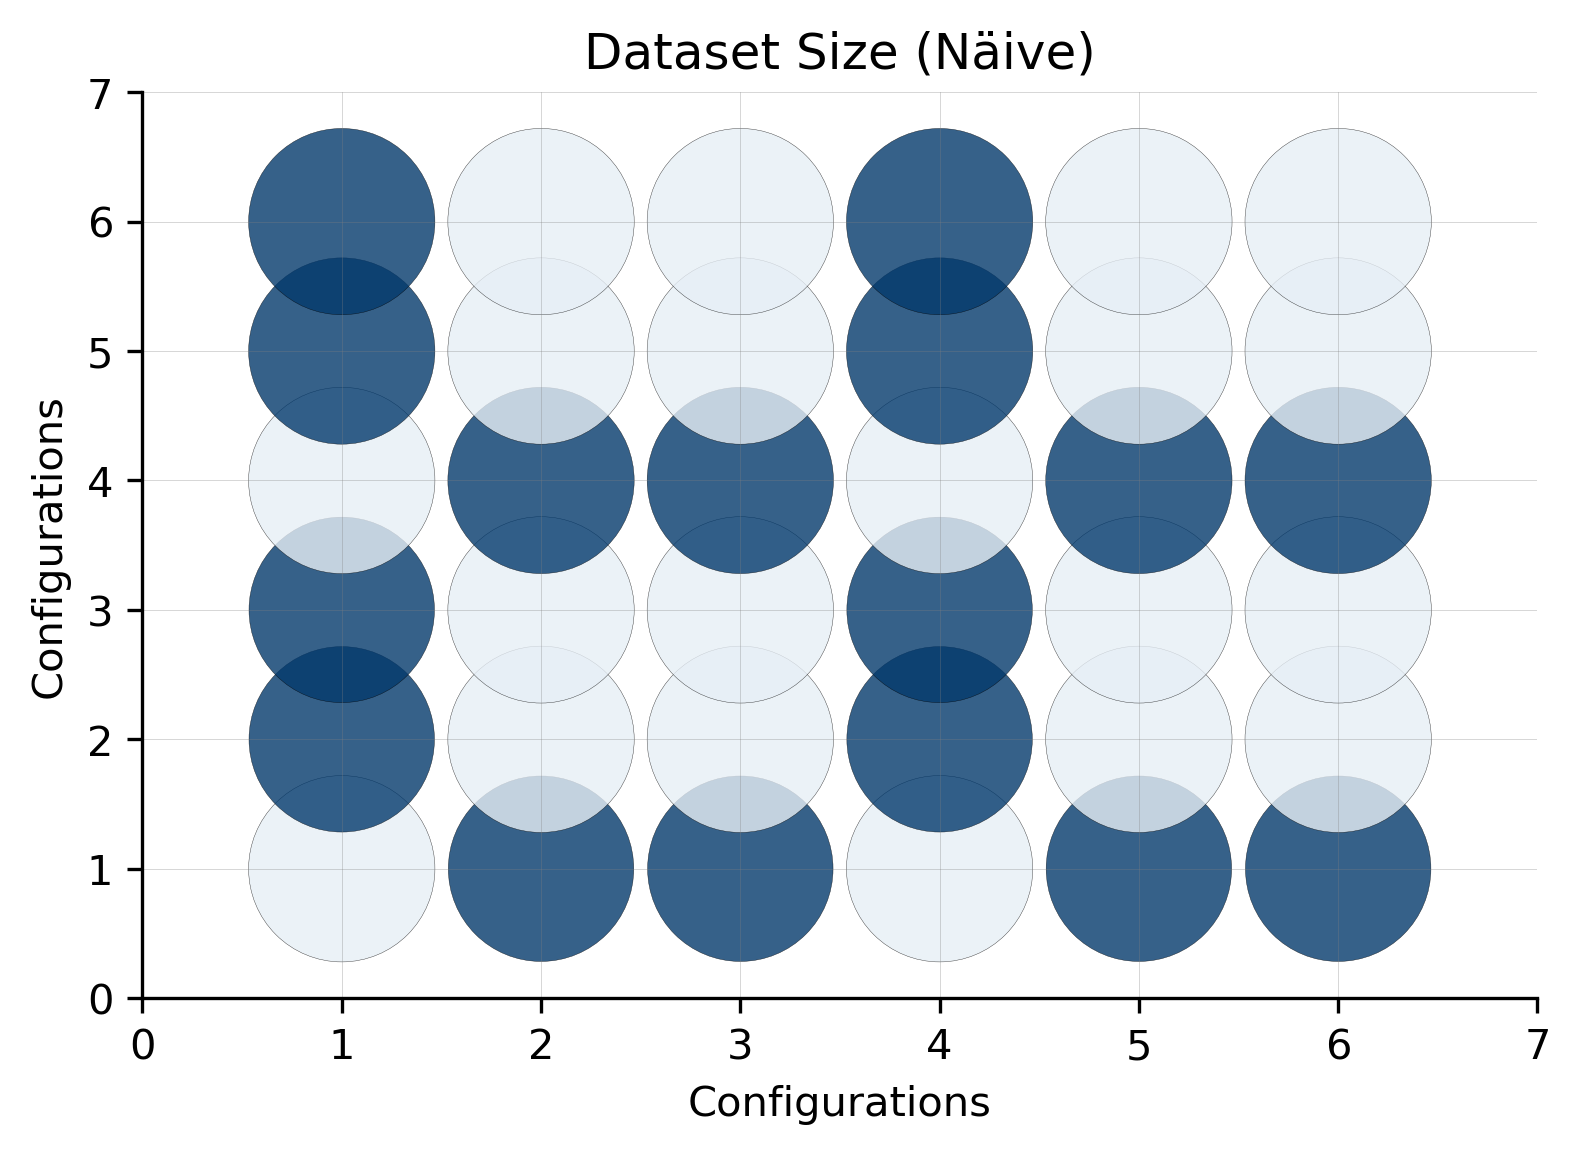
\includegraphics[width=0.8\columnwidth]{figures/naive_allk_bubble.png}
    \caption[Knowledge Graph Construction Tools on Different Dataset Sizes (Na{\"i}ve)]{\textbf{Comparison of Knowledge Graph Construction Tools on Different Dataset Sizes (Na{\"i}ve).} The first three configurations, i.e. 1, 2, and 3 in x-axis and y-axis, correspond to SDM-RDFizer on datasets 1K, 10K, and 50K, respectively. The last three configurations, i.e. 4, 5, and 6 on x-axis and y-axis, correspond to RMLMapper 1K, 10K, and 50K, respectively. Grey bubbles correspond to correlation value of $1.0$; blue bubbles show a positive correlation. The number of blue bubbles suggests that both systems exhibit similar behavior.}
    \label{fig:naive_bubble}
\end{figure}

\noindent \textbf{Configurations.}
We consider different configurations for the above-discussed variables in each dimension. 
%
\texttt{Dataset Size Configurations:} 1) SDM-RDFizer 1K; 2) SDM-RDFizer 10K; 3) SDM-RDFizer 50K; 4) RMLMapper 1K; 5) RML\-Mapper 10K; and 6) RMLMapper 50K. In each configuration of this parameter, we only use one data file.
%
\texttt{Relation Type configurations:} 1) SDM-RDFizer 1-N; 2) SDM-RDFizer N-1; 3) SDM-RDFizer N-M; 4) SDM-RDFizer Combinations (all relation types); 5) RMLMapper 1-N; 6) RMLMapper N-1; 7) RMLMapper N-M; and 8) RMLMapper Combinations (all relation types). For relation cardinality, we evaluated $N=\{1, 5, 10, 15\}$ and $M=\{1, 3, 5, 10\}$. In addition, we set the percentage of rows that involve in those relation types to $25\%$, i.e. $25\%$ of the overall rows from outer table have a matching join value to inner table, and $50\%$, respectively.
%
\texttt{Join Duplicate configurations:}  1) SDM-RDFizer Low, 2) SDM-RDFizer High, 3) RMLMapper Low, 4) RMLMapper High. \texttt{Low} Join Duplicates refer to datasets with low percentage of duplicates, i.e. from $5\%$ to $20\%$ of data generated could have duplicates due to the join conditions, similarly 
\texttt{High} Join Duplicates refer to higher percentage of duplicates, i.e. from $30\%$ to $50\%$ of data generated could be duplicated. 
%
\texttt{Join Selectivity Configurations:} 1) SDM-RDFizer High; 2) SDM-RDFizer Low; 3) RMLMapper High; and 4) RMLMapper Low. In this case, the join selectivity \texttt{High} represents how many time the join condition matches the values in the inner join file from 5\% to 20\% of the overall rows, while \texttt{Low} means that the join condition matches range from 60\% to 100\% of the overall number of rows. As previously shown, we hypothesise that these configurations allow us to uncover patterns in the behavior of these engines that could not be observed if only na{\"i}ve variables were studied. 

\noindent \textbf{Metrics}
We report on the following metrics or observed variables: 
\textit{Execution Time}: Elapsed time between execution of an engine and the delivery of the results.
\textit{Number of Results}: Number of triples generated by the KGC engine.

\noindent \textbf{Implementations.} 
The SDM-RDFizer and the testbeds are implemented in Python 3.6; the SDM-RDFizer is publicly available\footnote{\url{https://github.com/SDM-TIB/SDM-RDFizer}}. Furthermore, Jupiter Notebooks are available to generate the data and plot the results. Additionally, we have created a Docker image to run the testbeds and reproduce the experimental results\footnote{\url{https://github.com/SDM-TIB/KGC-Param-Eval}}. The experiments were run in an Intel(R) Xeon(R) equipped with a CPU E5-2603 v3 @ 1.60GHz 20 cores, 100G memory with Ubuntu 16.04LTS.


\begin{figure}[!tb]
    \centering
    \subfloat[Dataset 1K]{
      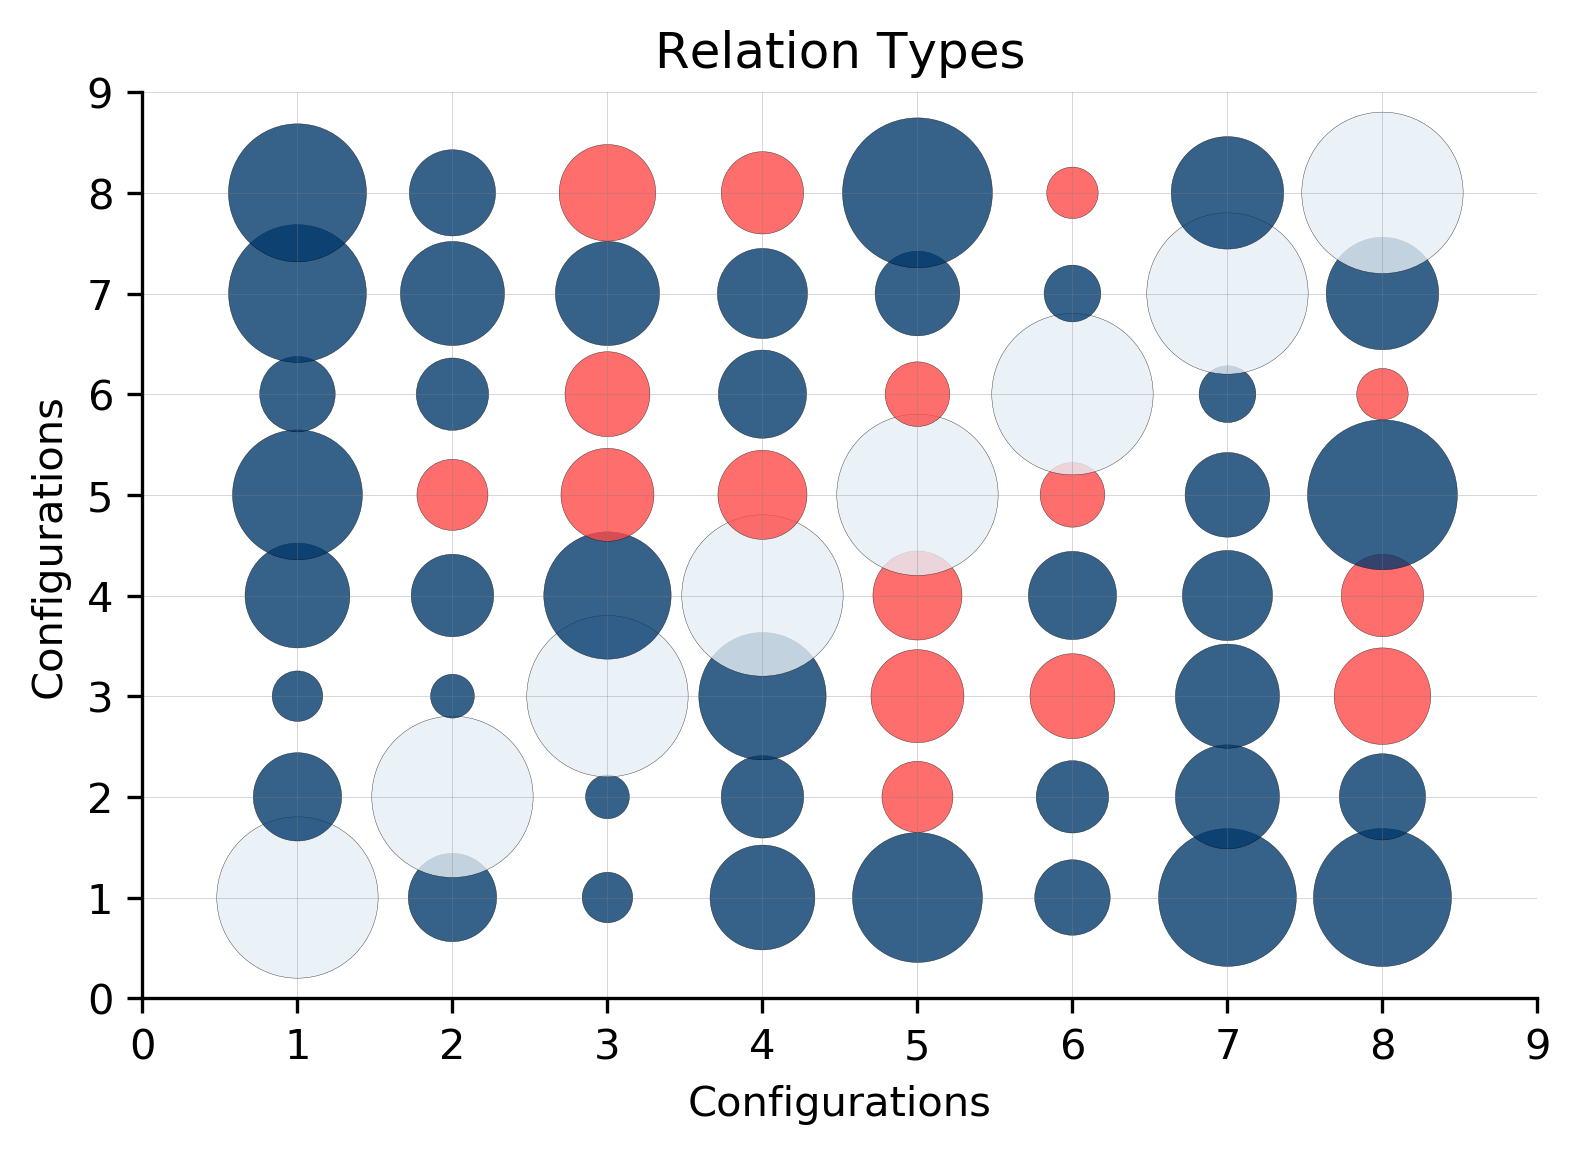
\includegraphics[width=0.48\columnwidth]{figures/relation_type_01k_bubble.png}
      \label{fig:rt_1k}
    }
    \subfloat[Dataset 10K]{
      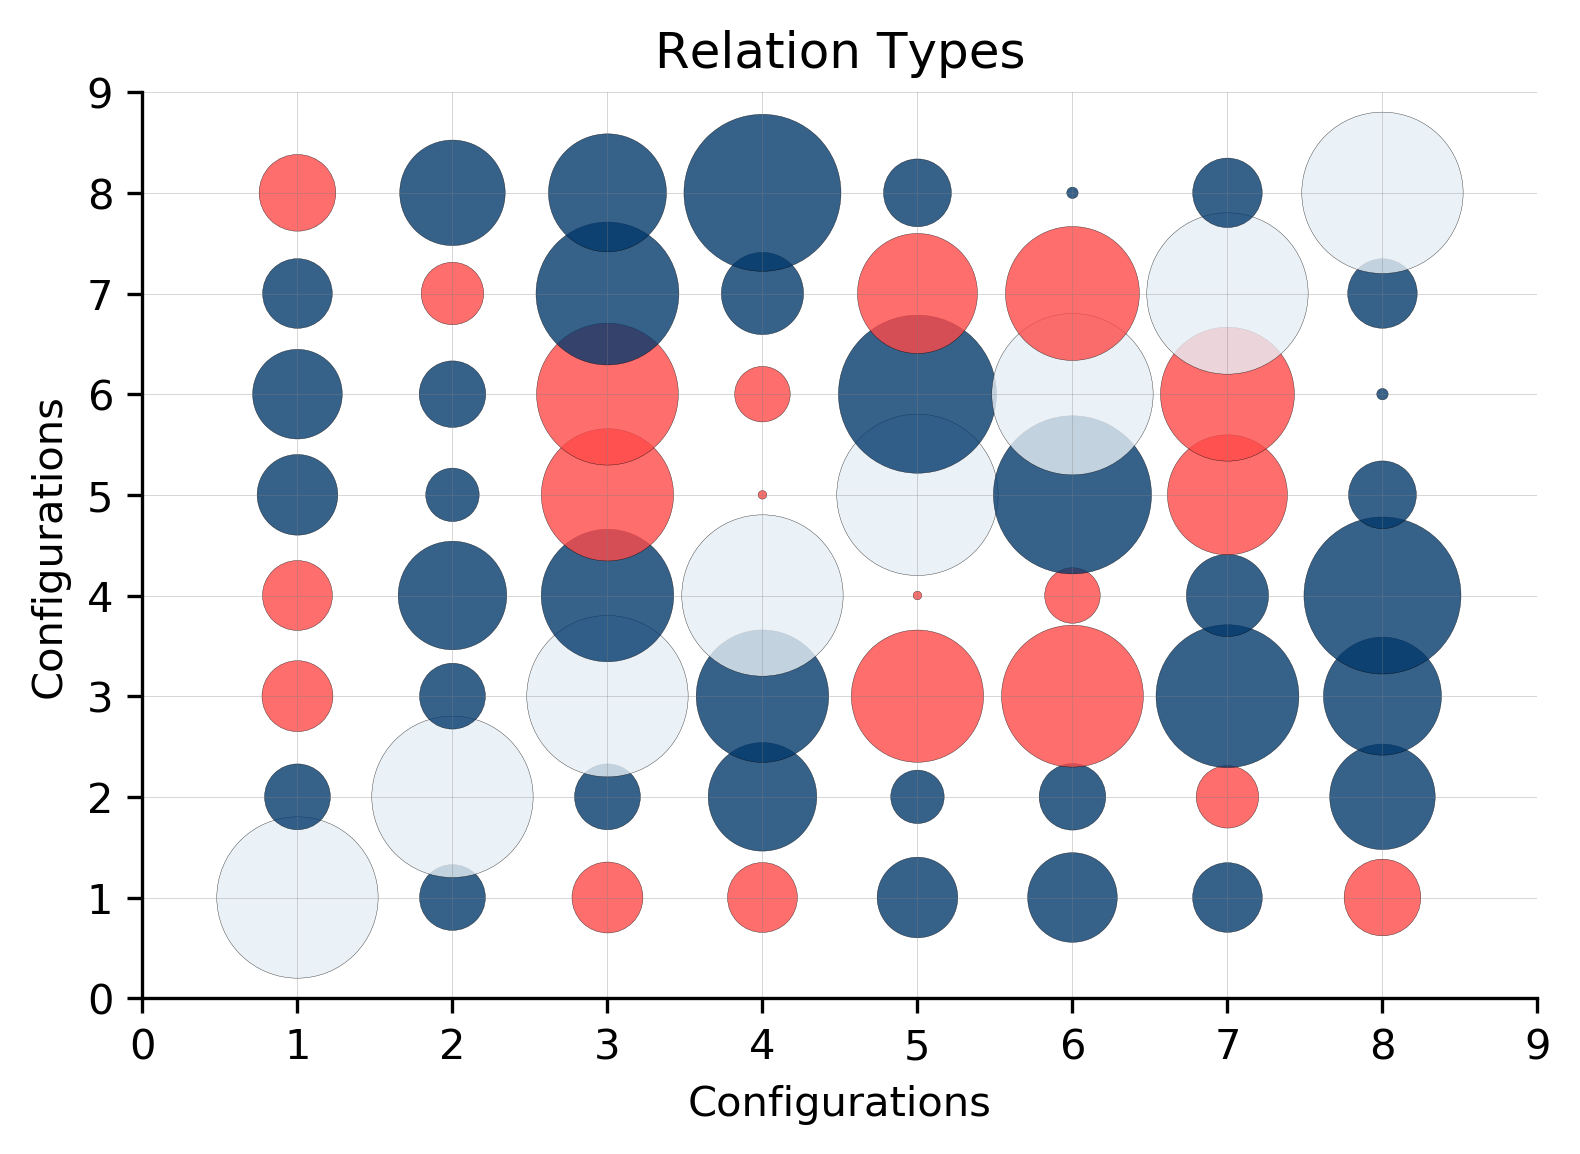
\includegraphics[width=0.48\columnwidth]{figures/relation_type_10k_bubble.png}
      \label{fig:rt_10k}
    }
    \qquad
    \subfloat[Dataset 50K]{
      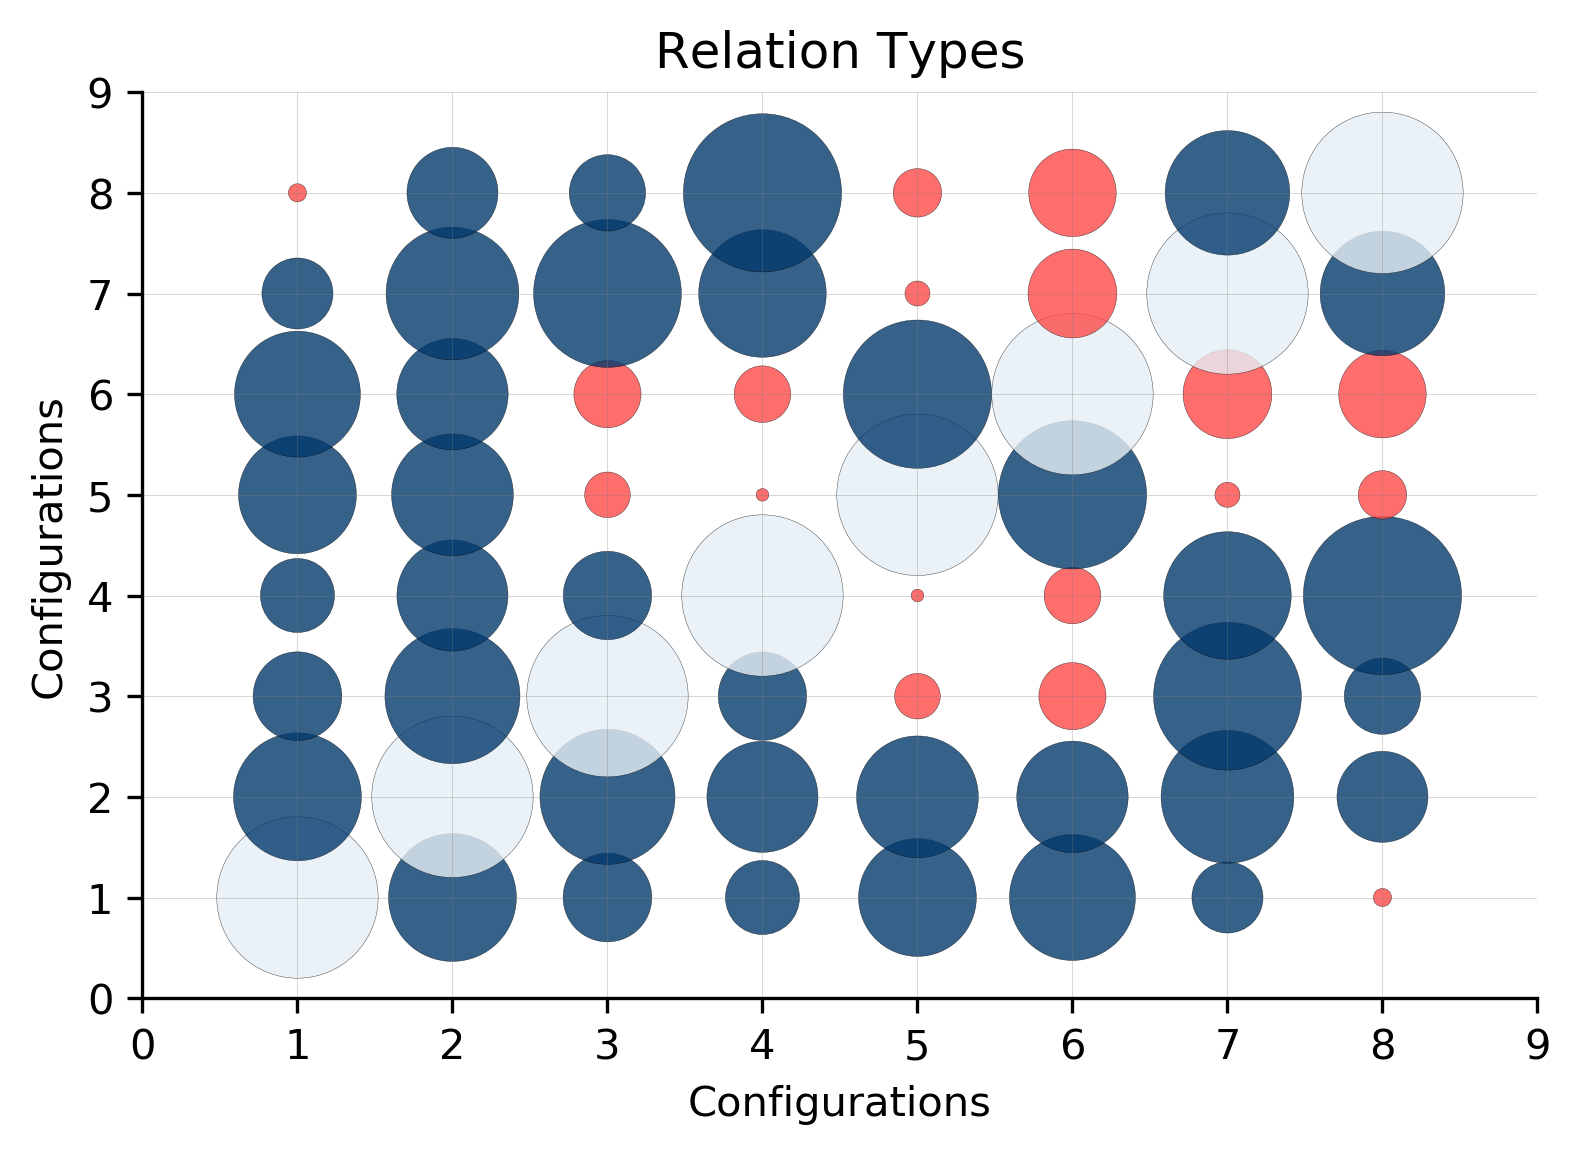
\includegraphics[width=0.48\columnwidth]{figures/relation_type_50k_bubble.png}
      \label{fig:rt_50k}
    }
    \subfloat[Combination of 1K, 10K, and 50K]{
      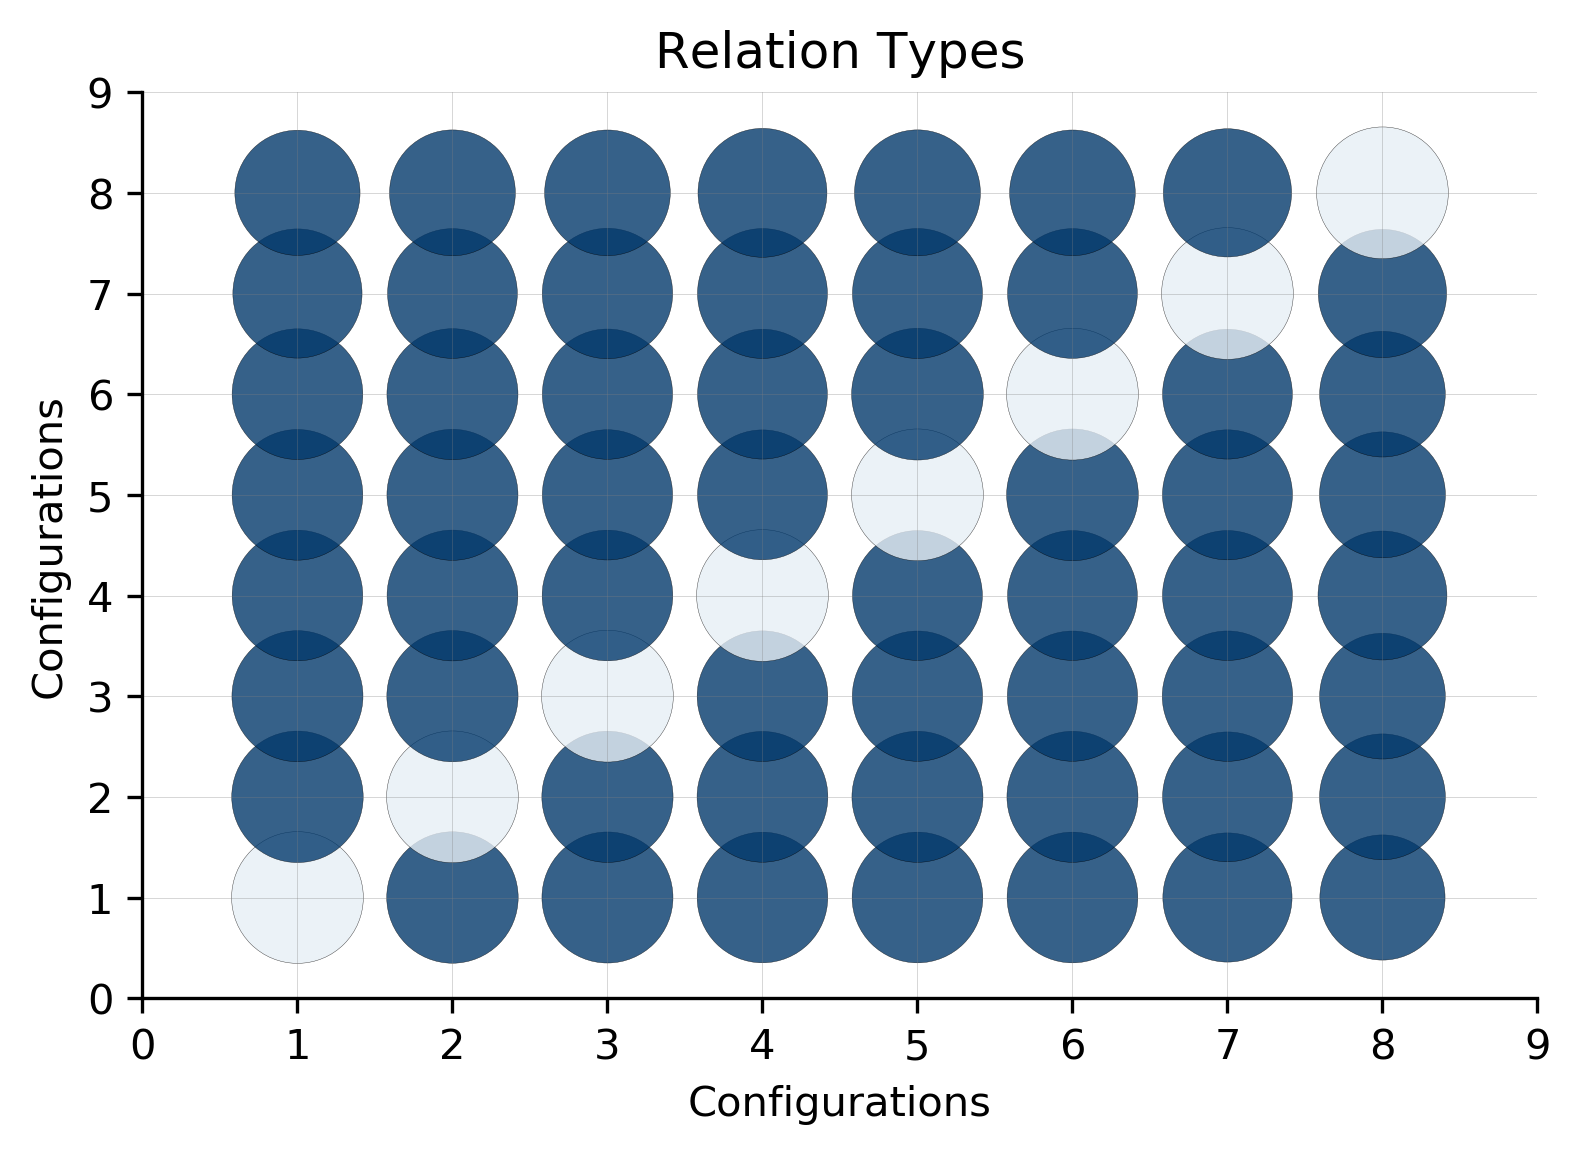
\includegraphics[width=0.48\columnwidth]{figures/relation_type_allk_bubble.png}
      \label{fig:rt_all}
    }
    \caption[Knowledge Graph Construction Tools on Different Types of Relations]{\textbf{Comparison of Knowledge Graph Construction Tools on Different Types of Relations.} The first four (4) configurations, i.e. 1-4 in both x-axis and y-axis, represent results of SDM-RDFizer on \textit{1-N}, \textit{N-1}, \textit{N-M}, and combination of all relations types, respectively. The later configurations, 5-8 both in x-axis and y-axis, shows results of RMLMapper on \textit{1-N}, \textit{N-1}, \textit{N-M}, and combination of all relations types, respectively. Grey bubbles correspond to correlation value of $1.0$; blue bubbles show a positive correlation while red bubbles show a negative correlation. The plots reveal that both type of relations and size of the dataset need to be taken into account to uncover patterns in the behavior of the engines. 
    }
    \label{fig:relation_type_bubble}
\end{figure}


\noindent \textbf{Testbeds.}
Results of each configurations are ordered from lower to higher complexity and compared using the Pearson's correlation. 
A high positive value of correlation between two configurations indicates that the corresponding engines had a similar behavior, i.e. the trends of execution time of the tools are similar; they are represented with blue bubbles in our plots. When a configuration is compared to itself, the Pearson's correlation reaches the highest value ($1.0$), represented with grey bubbles in our plots. 
On the other hand, a negative value indicates that there is an inverse correlation between the engines, i.e. they exhibit an opposite behavior; they are represented with red bubbles.


\subsubsection*{Discussion of the Observed Results}
We observe that the behavior of the engines can be affected when multiple variables are involved in a testbed (e.g. size and relation type) or when different levels of complexity of a variables (e.g. low, high join selectivity). We discuss the obtained results during our evaluation over the different configurations and parameters involved in each experiment:   

\noindent \textbf{Dataset Size (Na{\"i}ve):}
Figure~\ref{fig:naive_bubble} depicts the comparison of engines when the dataset size is considered. When \texttt{configuration 1} is compared to itself, the Pearson's correlation value is $1.0$; additionally, it is high and positive when it is compared to \texttt{configurations 2, 3, 5, and 6} (large blue bubbles). 
Using this parameter, the correlation analysis suggests that both engines behave similarly in all configurations. Moreover, this indicates that only considering the data size is not enough to uncovered the properties of the studied engines.


\begin{figure}[!tb]
    \centering
    \subfloat[Dataset 1K]{
      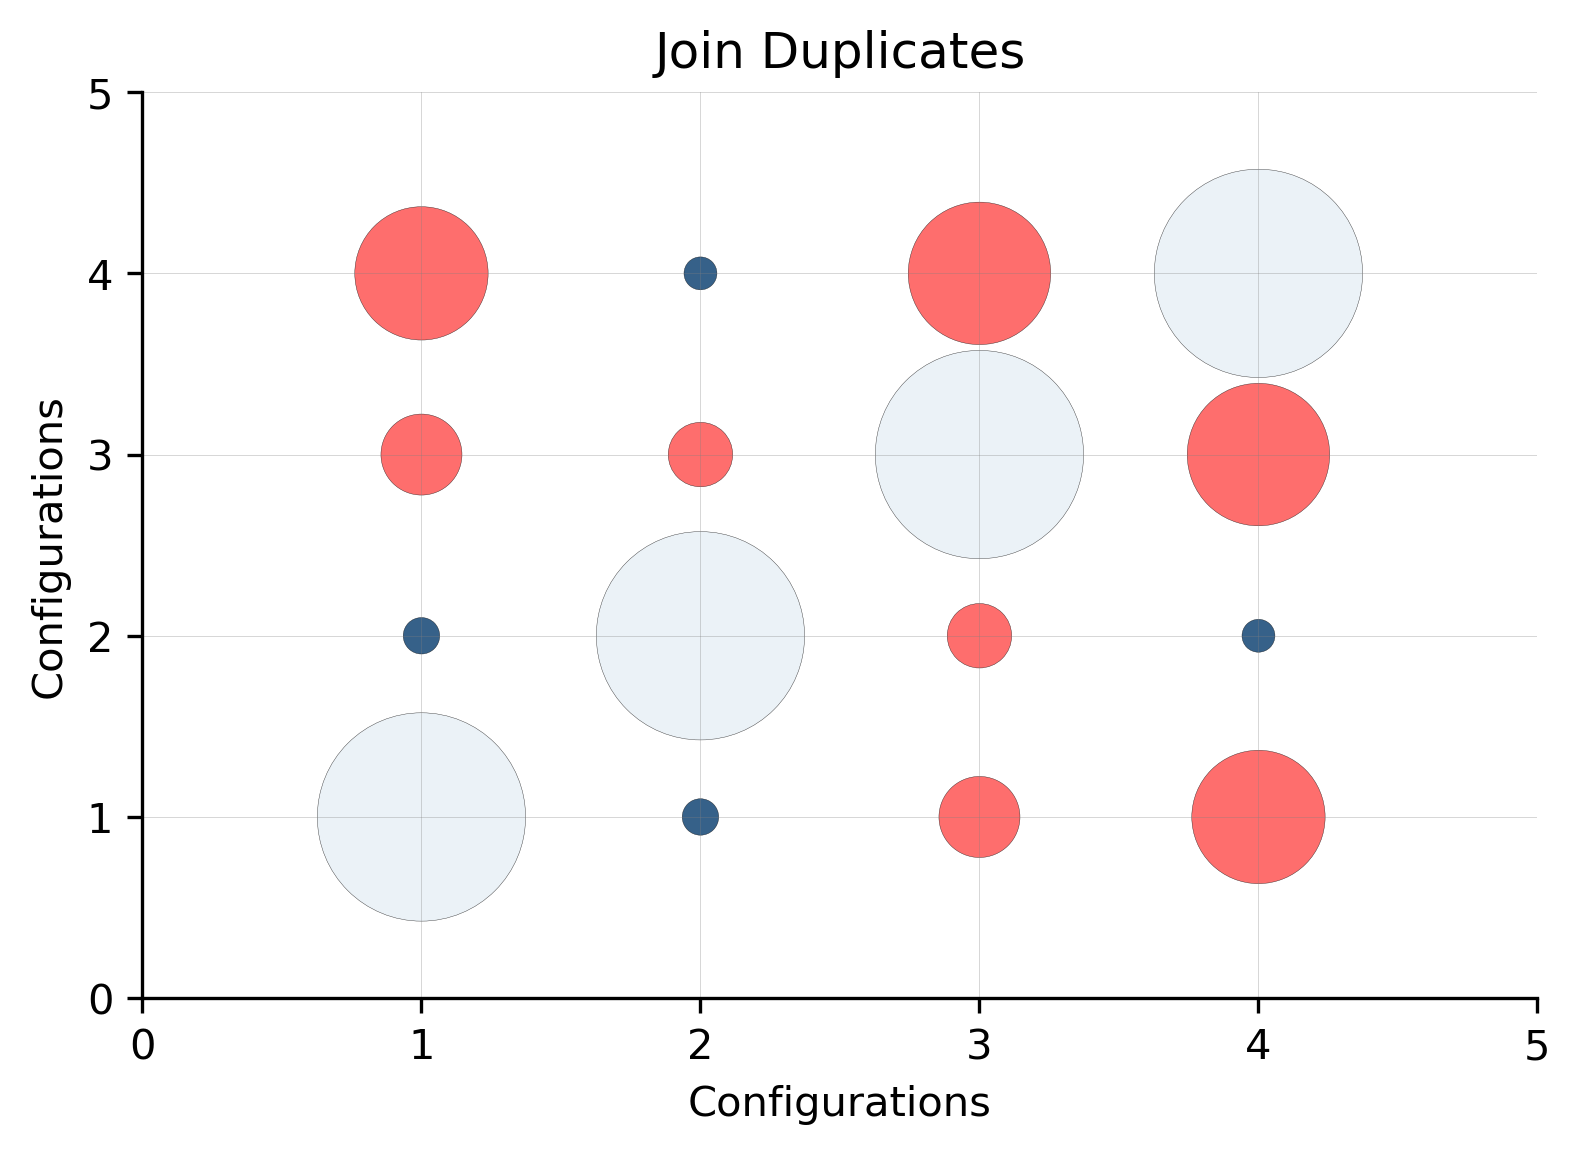
\includegraphics[width=0.48\columnwidth]{figures/duplicate_joins_01k_bubble.png}
      \label{fig:naive1}
    }
    \subfloat[Dataset 10K]{
      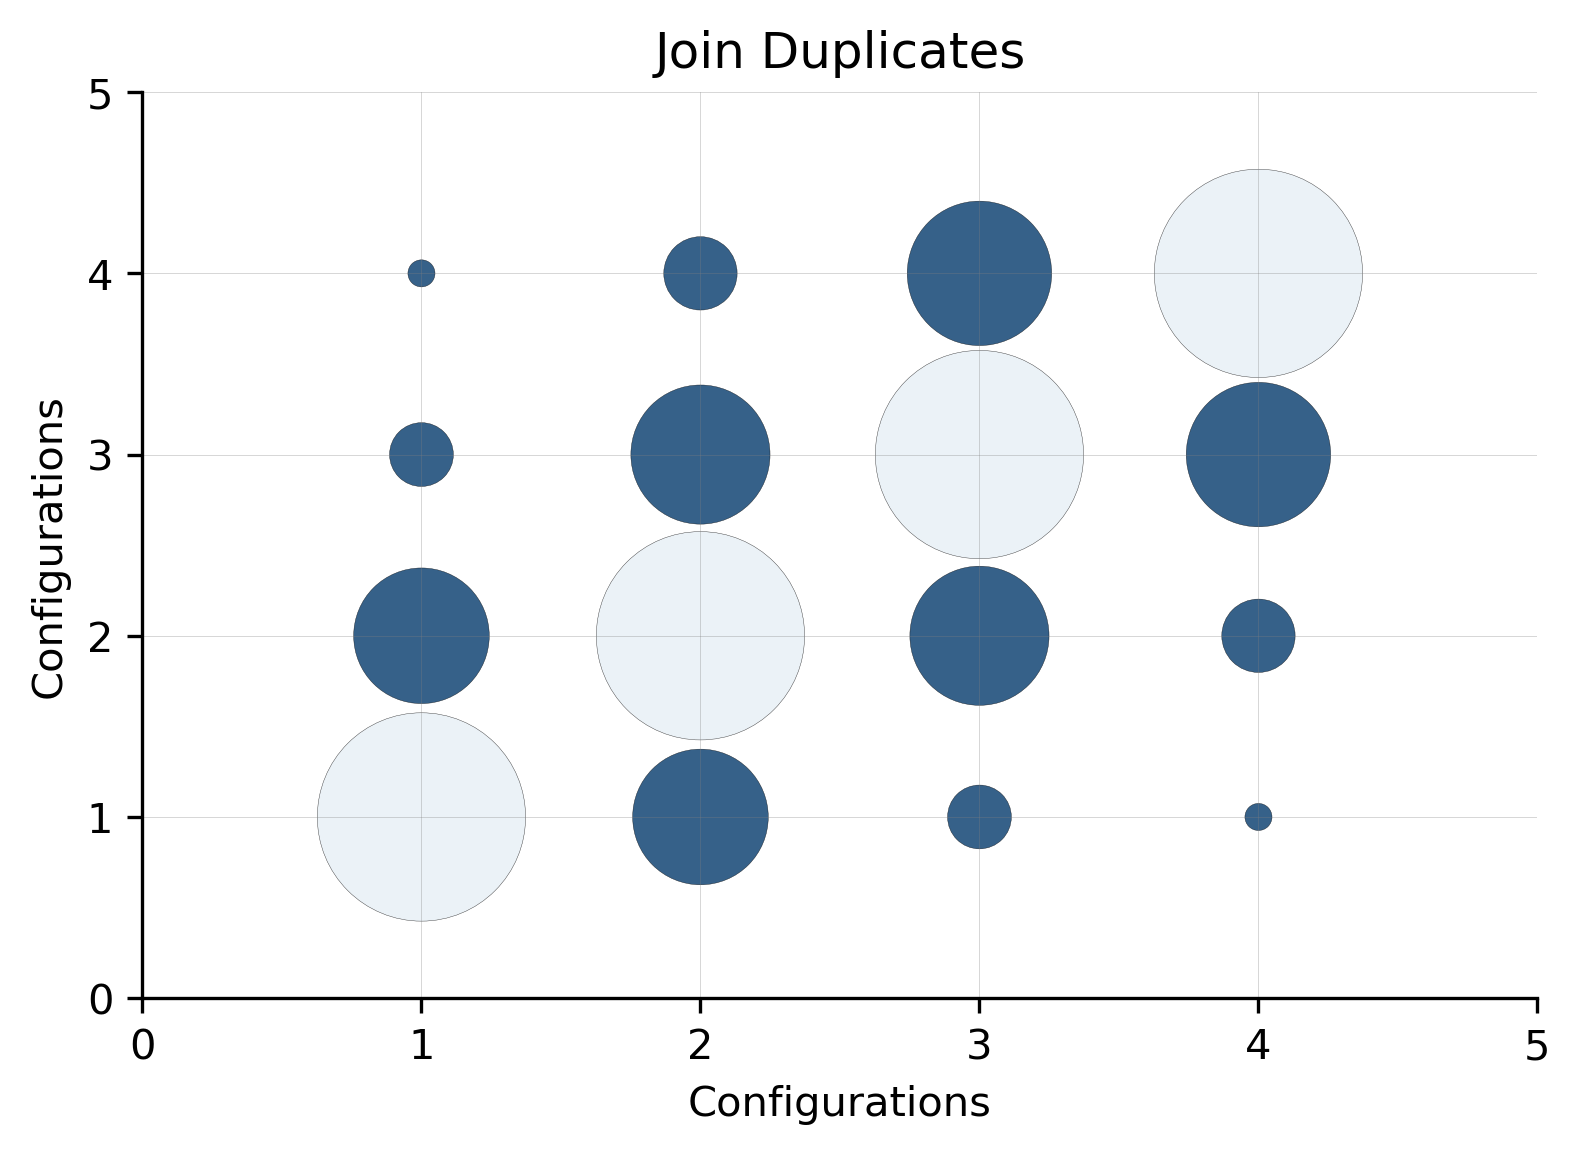
\includegraphics[width=0.48\columnwidth]{figures/duplicate_joins_10k_bubble.png}
      \label{fig:js0}
    }
    \qquad
    \subfloat[Dataset 50K]{
      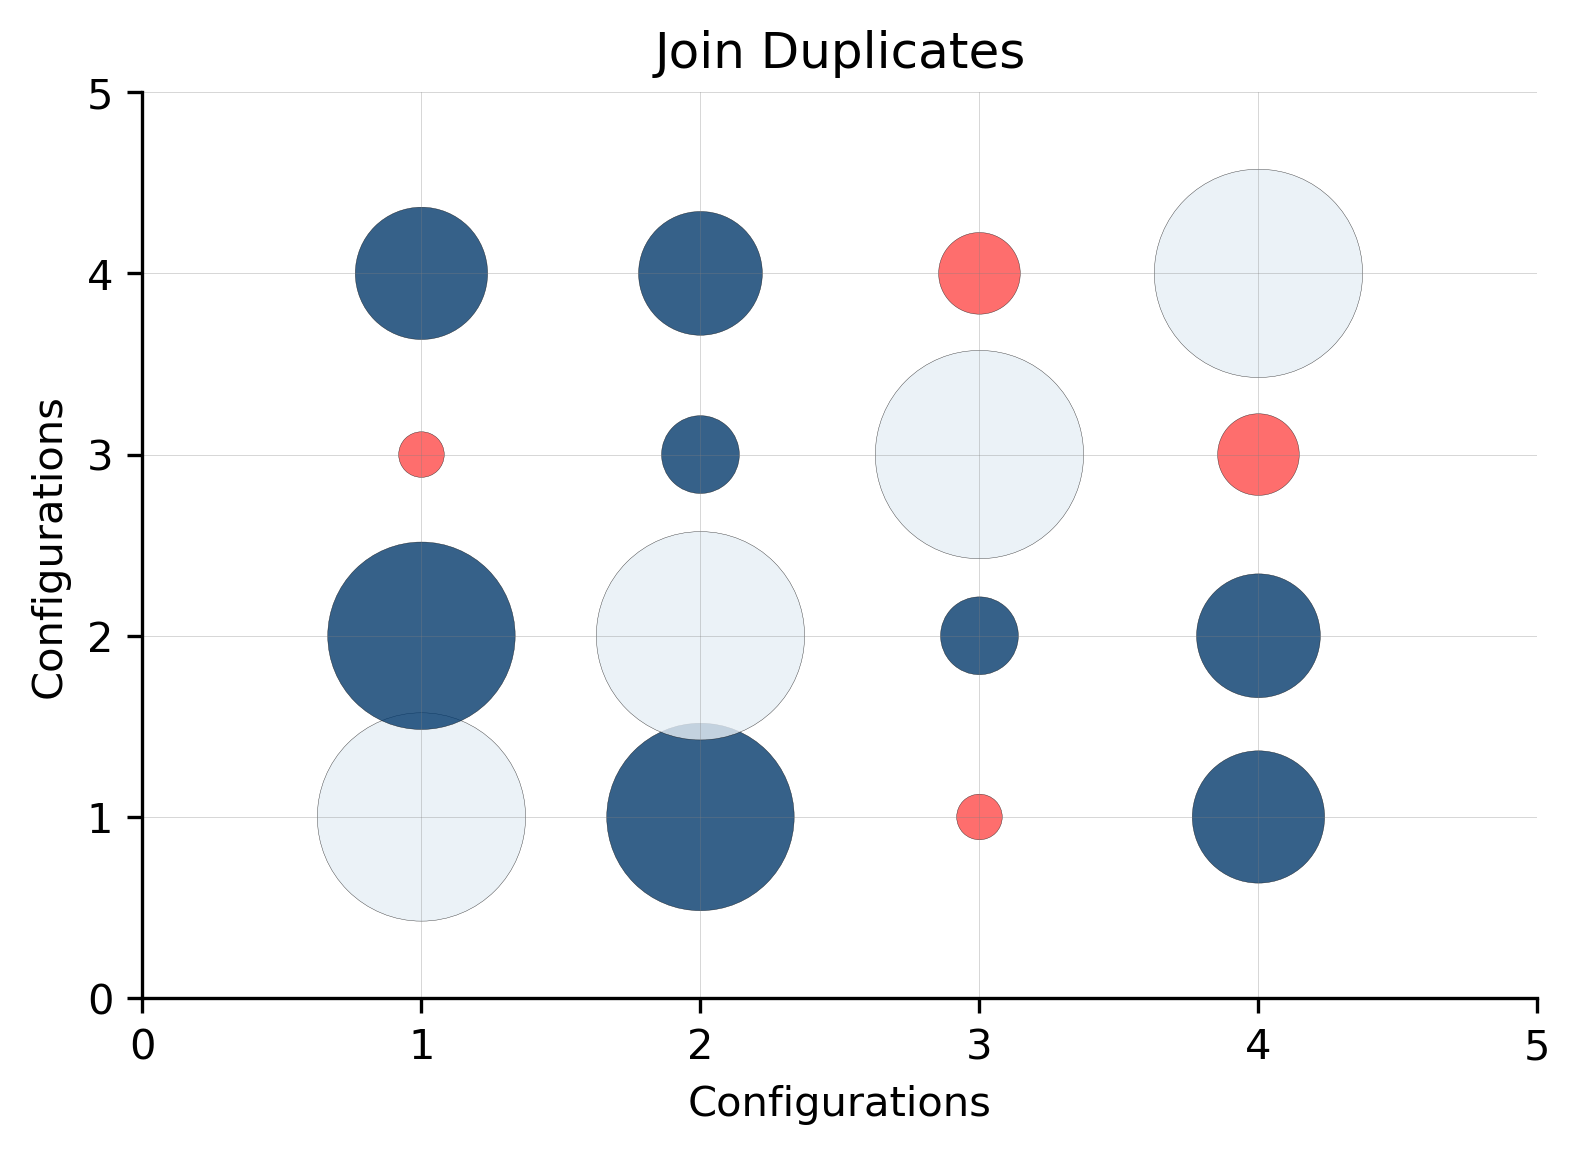
\includegraphics[width=0.48\columnwidth]{figures/duplicate_joins_50k_bubble.png}
      \label{fig:naive2}
    }
    \subfloat[Combination of 1K, 10K, and 50K]{
      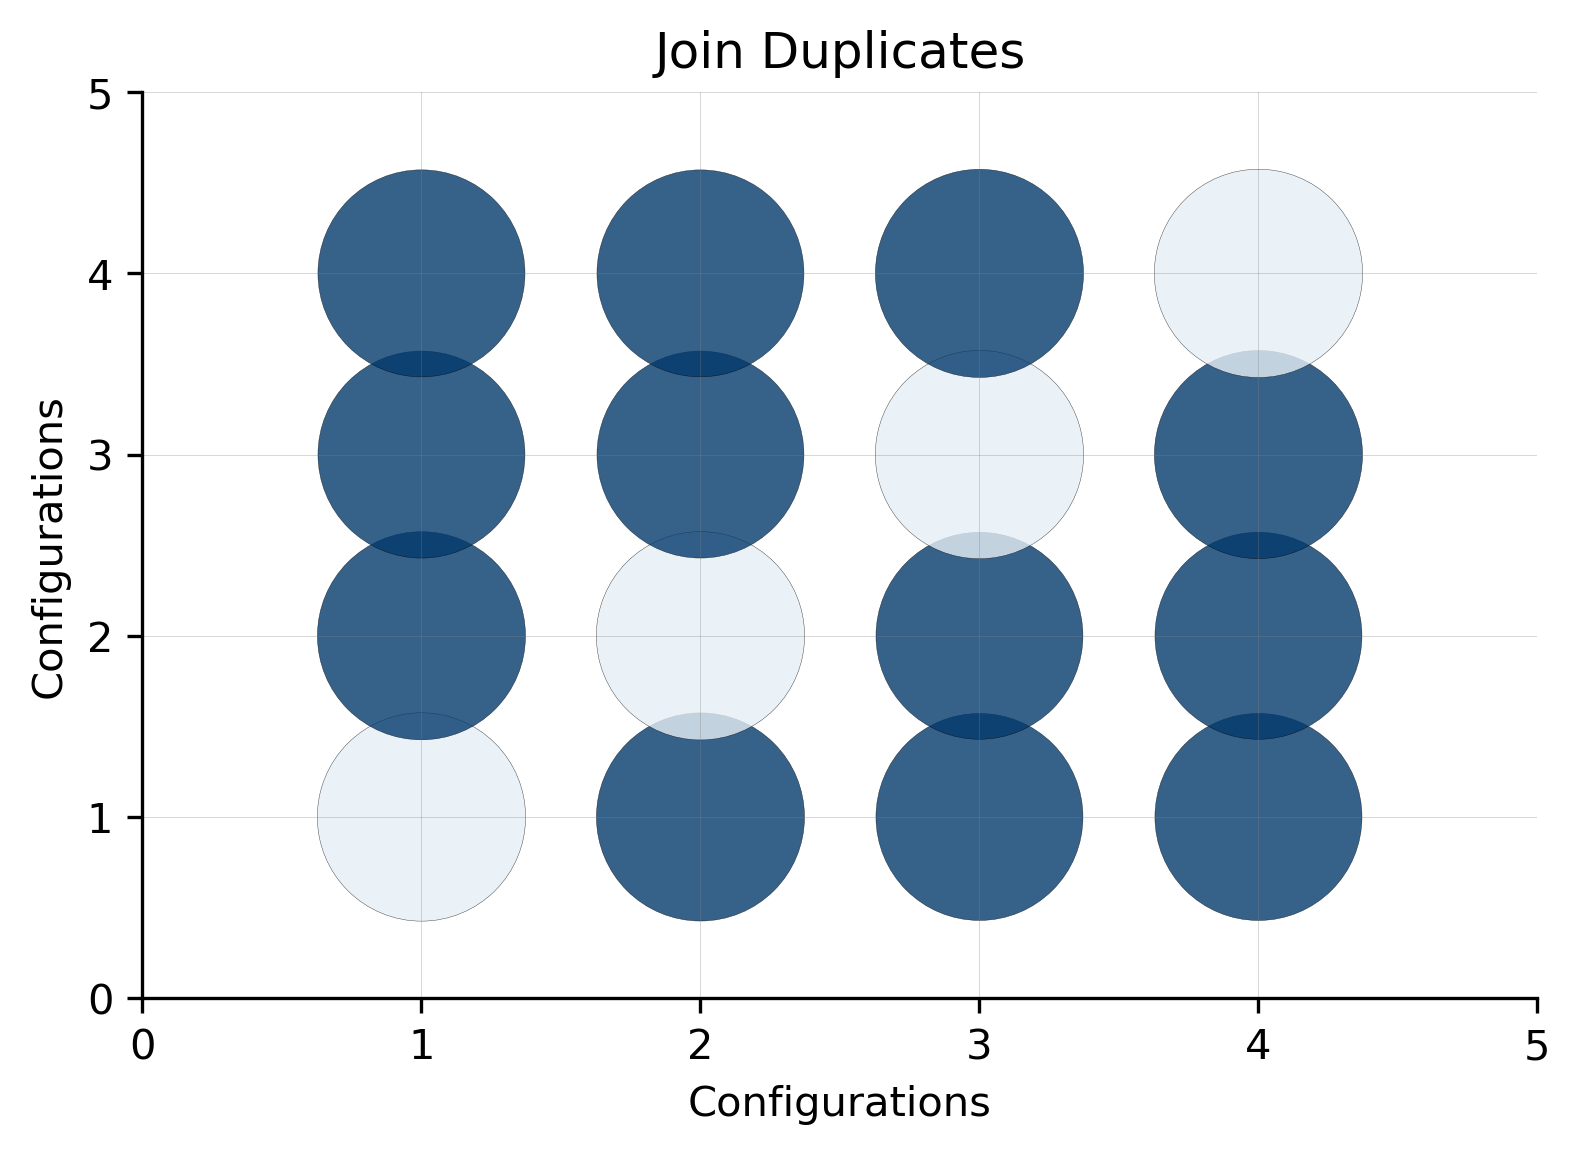
\includegraphics[width=0.48\columnwidth]{figures/duplicate_joins_allk_bubble.png}
      \label{fig:js1}
    }
    \caption[Knowledge Graph Construction Tools on Duplicates during Join]{\textbf{Comparison of Knowledge Graph Construction Tools on Duplicates during Join.} The first two (2) configurations, i.e., 1-2 on x-axis and y-axis, represent results of SDM-RDFizer on datasets with \textit{low} (5\%-20\% of data) number of duplicates and \textit{high} (30\%-50\% of data) number of duplicates generated during joins, respectively. The last two configurations, i.e., 3-4 on x-axis and y-axis, represent results of RMLMapper on datasets with \textit{low} number of duplicates and \textit{high} number of duplicates generated during joins, respectively. Grey bubbles correspond to correlation value of $1.0$; blue bubbles show a positive correlation while red bubbles show a negative correlation. Results evidence that both join duplicates and dataset size are needed for characterising an engine performance.}
    \label{fig:duplicates_bubble}
\end{figure}


\begin{figure}[!tb]
    \centering
    \subfloat[Dataset 1K]{
      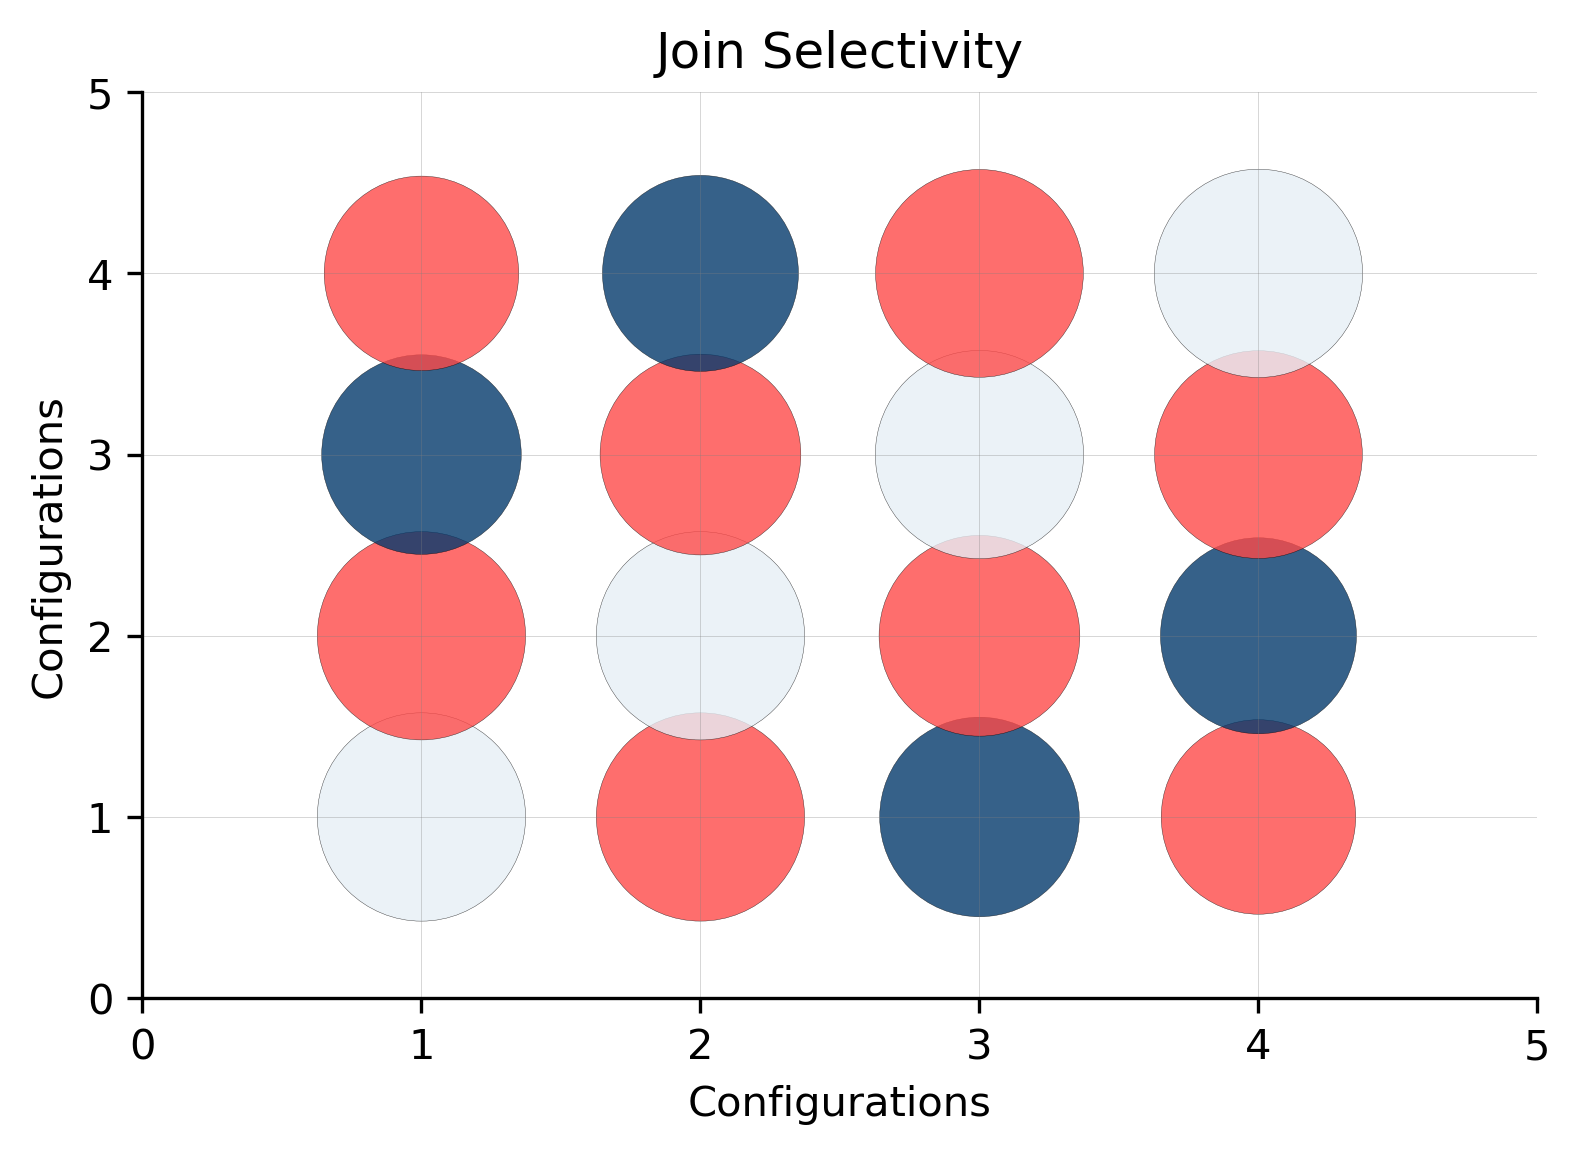
\includegraphics[width=0.48\columnwidth]{figures/join_selectivity_01k_bubble.png}
      \label{fig:naive3}
    }
    \subfloat[Dataset 10K]{
      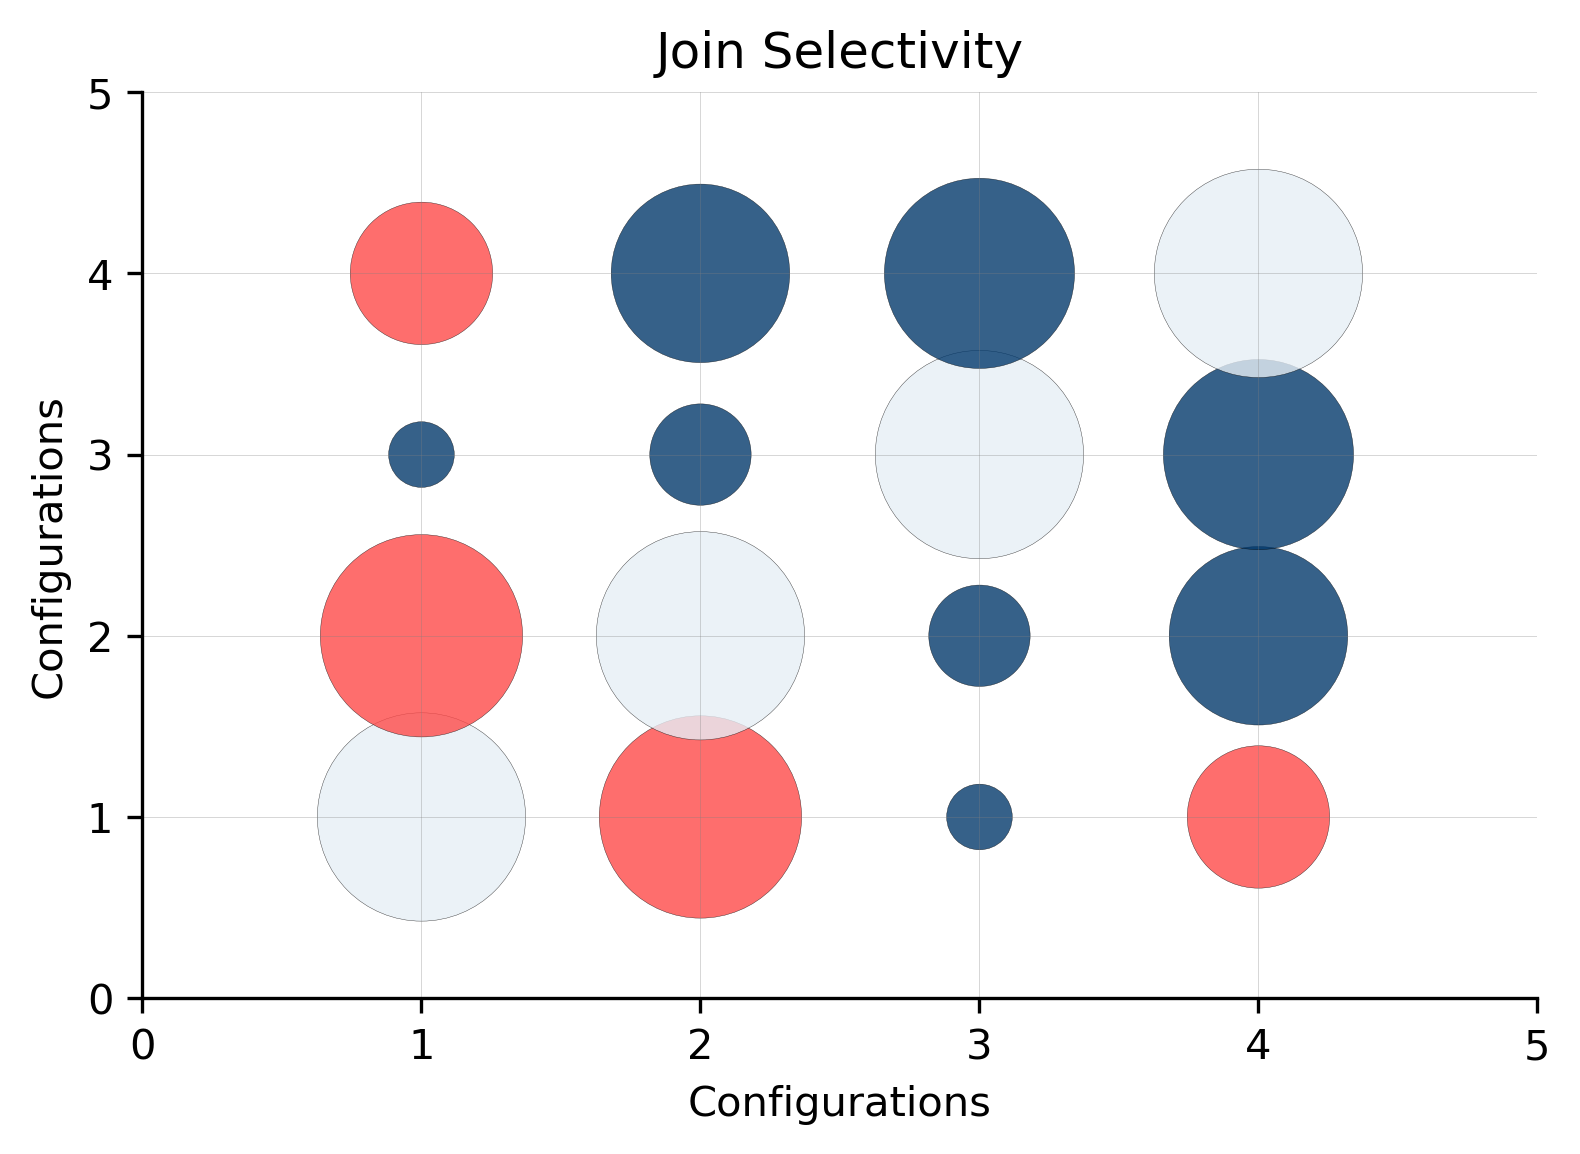
\includegraphics[width=0.48\columnwidth]{figures/join_selectivity_10k_bubble.png}
      \label{fig:js3}
    }
    \qquad
    \subfloat[Dataset 50K]{
      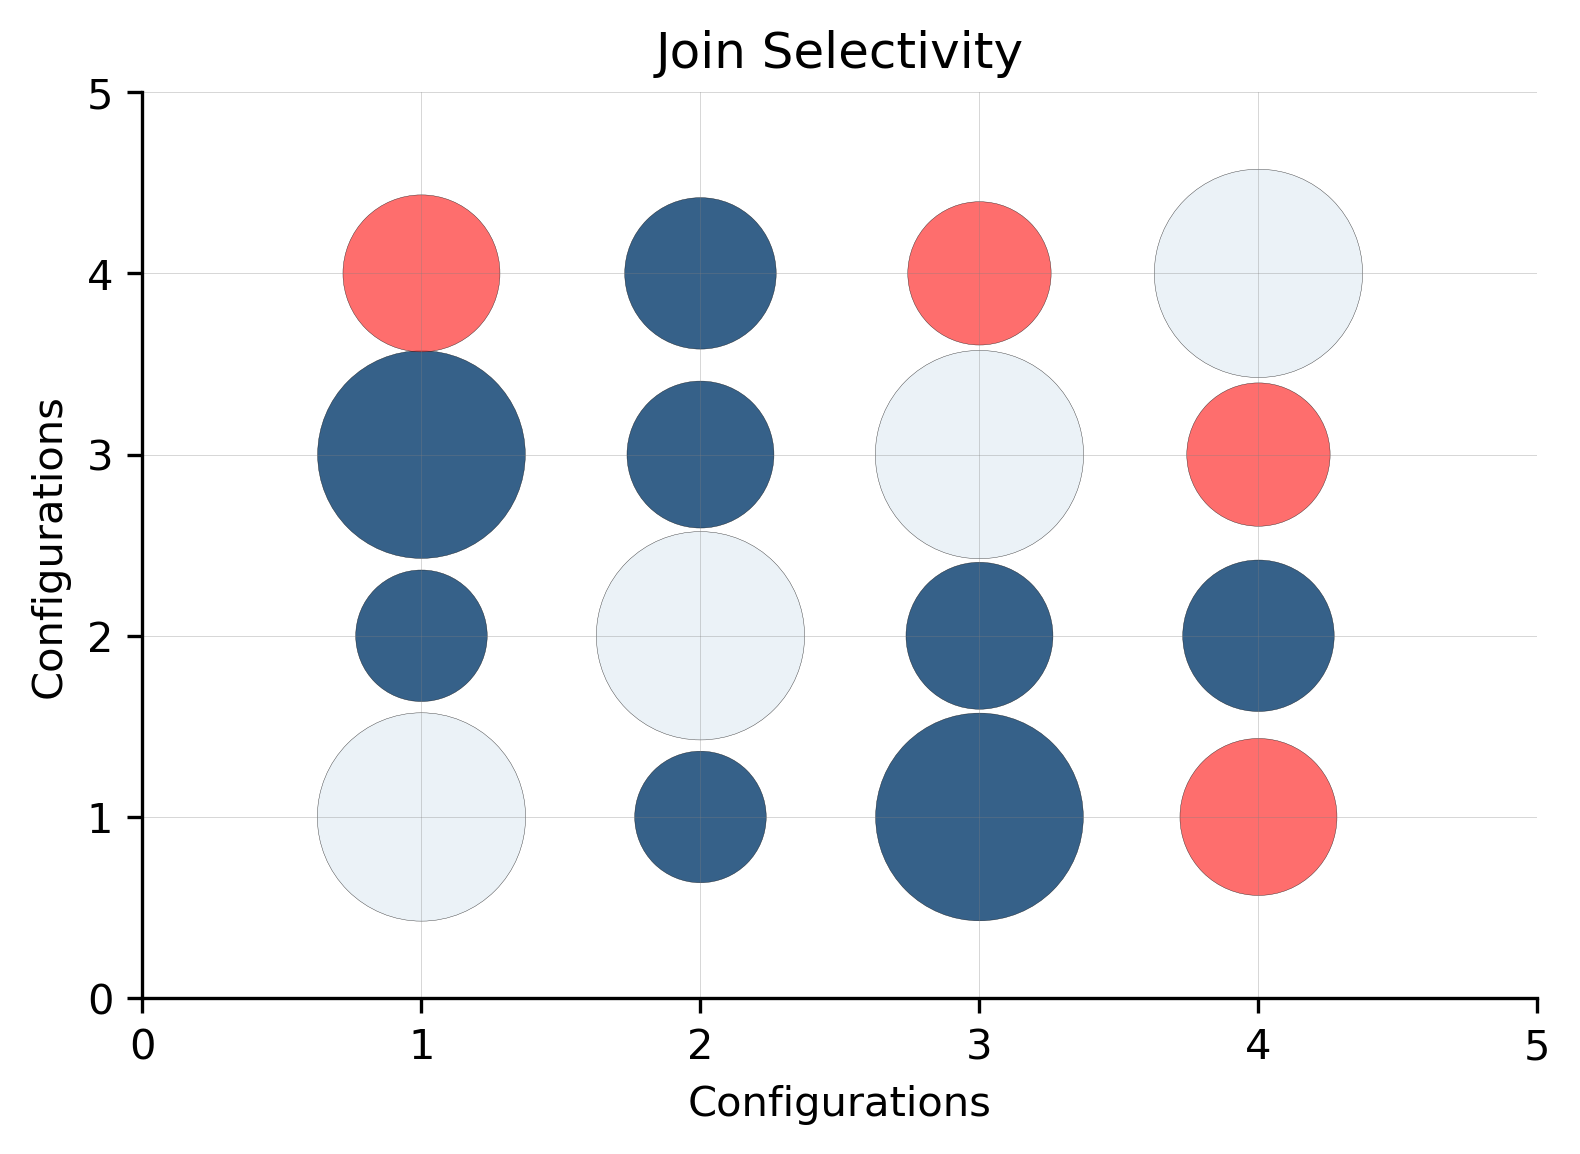
\includegraphics[width=0.48\columnwidth]{figures/join_selectivity_50k_bubble.png}
      \label{fig:naive4}
    }
    \subfloat[Combination of 1K, 10K, and 50K]{
      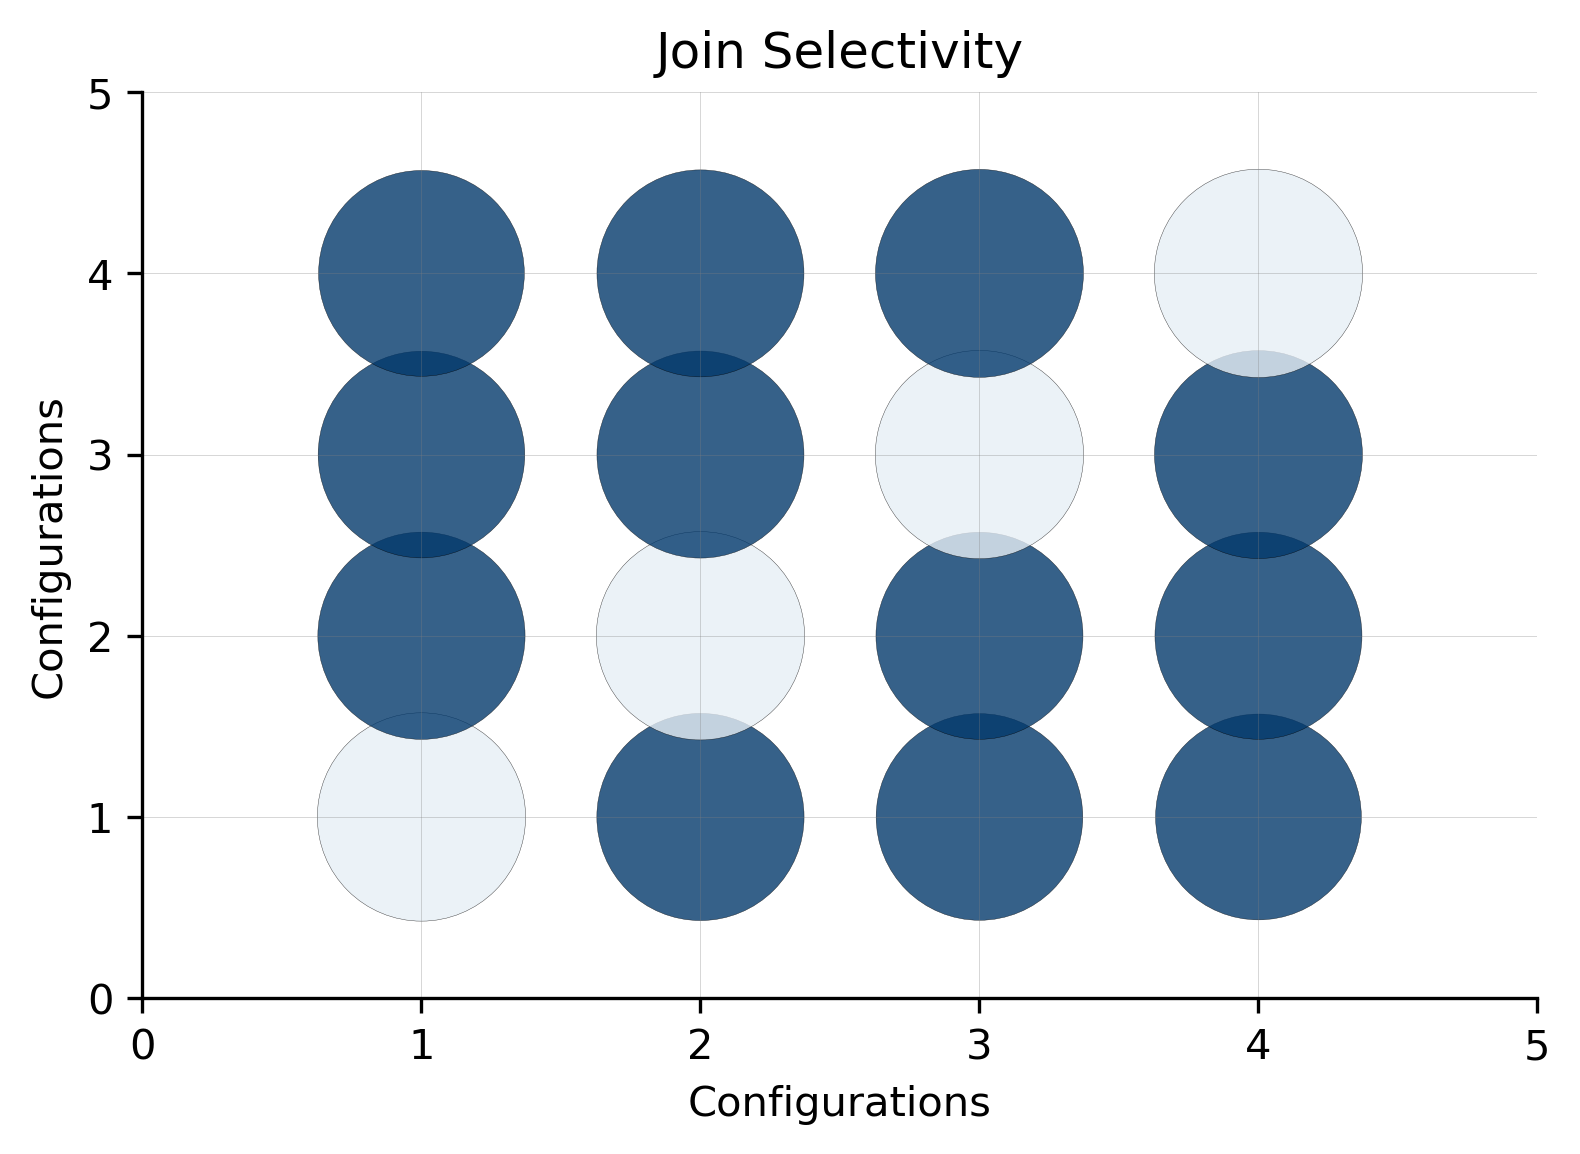
\includegraphics[width=0.48\columnwidth]{figures/join_selectivity_allk_bubble.png}
      \label{fig:js4}
    }
    \caption[Knowledge Graph Tools on Join Selectivity]{\textbf{Comparison of Knowledge Graph Tools on Join Selectivity.} The first two configurations, i.e., 1-2 on x- and y-axis represent SDM-RDFizer on joins with \textit{high} selectivity (5\%-20\% of data) and joins with \textit{low} selectivity (60\%-100\% of data), respectively.  Configurations 3 and 4 represent RMLMapper on joins with \textit{high} selectivity (5\%-20\% of data) and joins with \textit{low} selectivity (60\%-100\% of data), respectively. Grey bubbles correspond to correlation value of $1.0$; blue bubbles show a positive correlation while red bubbles show a negative correlation. Dataset size and join selectivity affect both engines differently.}
    \label{fig:joinselectivity_bubble}
\end{figure}



\noindent \textbf{Relation Types:}
Figure~\ref{fig:relation_type_bubble} reports on the correlation of different configurations for various join relation types. We can observe in Figures \ref{fig:rt_1k}, \ref{fig:rt_10k}, and \ref{fig:rt_50k} several red bubbles, indicating a negative correlation in the behavior of the compared configurations and engines. Contrary, Figure \ref{fig:rt_all} does not depict any red bubble, suggesting thus, that the two engines in all the configurations exhibit the same behavior. These results clearly illustrate the need of considering different configurations and parameters in order to avoid drawing wrong conclusions about the main characteristics of existing tools. 


\noindent \textbf{Join Duplicates:}
Figure~\ref{fig:duplicates_bubble} depicts the correlation between different configurations when different setting of duplicates are produced during the execution of joins between triple maps. As can be observed, Figures \ref{fig:naive1}, and \ref{fig:naive2} include several red bubbles that indicate an opposite behavior of the engines. Contrary, Figures \ref{fig:js0}, and \ref{fig:js1} suggest that both engines behave similarly. 


\noindent \textbf{Join Selectivity:}
Figure~\ref{fig:joinselectivity_bubble} shows the correlation between different configurations for the selectivity of join conditions. Similarly, these testbeds reveal contradicting patterns in the behaviors of the studied engines. On one hand, Figures \ref{fig:naive3}, \ref{fig:js3}, and \ref{fig:naive4} are composed of several red bubbles and indicate that these engines perform differently whenever the selectivity of the join condition is changed. Surprisingly,  when the size of these datasets are also taken into account in the testbed (Figure \ref{fig:js4}), these patterns are hidden, and the results of the evaluation suggest that both engines perform similarly whenever the selectivity of the join condition is changed. 

The results reported in this experimental study provide clear evidence of the importance of the variables and configurations that composed the methodology devised in this work. Actually, in the four studied cases, they reveal important patterns that could not be observed whenever other parameters were studied simultaneously. Based on these observations, we can conclude that these variables and configurations should be included in the benchmarks in order to ensure that the characteristics of knowledge graph construction engines are uncovered. Thus, these observations allow us to answer our three research questions: \textbf{RQ1}, \textbf{RQ2}, and \textbf{RQ3}. We encourage developers and users of knowledge graph construction tools to bear in mind them during benchmarking in order to draw clear conclusions about the performance of their tools.


\subsection{Conclusions}
In this section, we performed an in-depth analysis of the variables and configurations that impact on the behavior of two engines. The observation that existing engines exhibit heterogeneous behaviors whenever small changes in the testbeds are conducted, motivated the need of conducting this study involving a set of parameters that can reveal patterns in the behavior of the studied engines. Additionally, the lack of testbeds encouraged us to acquit the definition of variables and configurations that enable for the characterization of the pitfalls of existing engines and for identifying the list of challenges and research directions in the state of the art. 
With the proposed analysis and the results of the experimental study, we contribute with an empirical configuration that can be reused for the evaluation of other knowledge graph construction tools and mapping languages (e.g., SPARQL-Generate, TARQL, or R2RML). Furthermore, our set of variables and configurations can be utilized as a guideline during testing and benchmarking. One of the main lessons learned during the definition and evaluation of our approach, is that none of the evaluated engines behaves consistently whenever the complexity of the testbeds increases. Our ambition is that the reported results inspire the community to define general testbeds that facilitate the understanding of the state of the art and the development of novel tools for the construction of knowledge graphs at large scale.  In the future, we plan to define testbeds and conduct a more detailed analysis of other engines and mapping languages. Moreover, we envision to motivate the community to conduct a joint effort in the definition of benchmarks that enable for fair evaluations of knowledge graph construction tools with replicable and generalizable results. 


\section{GTFS-Madrid-Bench: Evaluation of Virtual Knowledge Graph Access}

%Over the last few years, a growing number of datasets have been made available in various open data portals. For example, the European Data Portal\footnote{https://www.europeandataportal.eu/catalogue-statistics/CurrentState} aggregates, at the time of writing, approximately 500K datasets from EU countries in a diversity of domains. In this context, RDF has been proposed as a standard format for data interchange on the Web, and RDF Schema and OWL ontologies have begun to appear so as to provide shared models in some domains. However, the amount of non-RDF data (e.g., CSV, JSON, XML) that is published in these open data portals continues to dominate the scene (see Table \ref{tab:odp}) and interoperability issues hinder their (re)use and consumption. 

%Data integration is not a new problem but it is exacerbated by the availability of such open data on the Web, that is, it was already identified and addressed several decades ago with an emphasis on data in relational databases. Different techniques and tools have been used to address this problem. In our work, we focus on those based on ontologies. In Ontology Based Data Access (OBDA)~\citep{poggi2008linking} data consumers issue queries over a dataset according to a common unified view (an ontology). The information needed to reformulate the queries is usually available in the form of declarative mappings. In Ontology Based Data Integration (OBDI)~\citep{poggi2008linking}, these techniques are expanded to address heterogeneous datasets, whose data needs to be integrated to provide answers to these queries. In both ontology-based approaches, two different alternatives exist to enable data access: (1) those where data are materialised taking into account the mappings and the ontologies (for example, data is transformed into RDF and loaded into a triple store, so that it can be queried using SPARQL), and (2) those where the transformation is done on the queries, which can then be evaluated on the original data sources. This last alternative is the one considered for our work because it removes the need for materialisation, something especially useful for very dynamic data sources~\citep{corcho2019towards}. We refer to it as ``virtualized knowledge graph access''.

%To facilitate data exploitation in this context, application developers need to understand the strengths and weaknesses of existing data integration tools. Additionally, tool developers may want to know if their engines cover the requirements of real use-case scenarios. In both cases the challenge is to develop a benchmark that covers the requirements of ``virtualized knowledge graph access''  and that is extensible and sustainable over time. In general, it is  necessary to have an overview of state of the art engines that are tailored to different source formats, accepting as input mappings that are represented in a variety of declarative languages.

%Several benchmarks already exist in the state of the art of OBDA~\citep{bizer2009berlin,lanti2015npd}, as well as in SPARQL query federation~\citep{schmidt2011fedbench,hasnain2017biofed,montoya2012benchmarking}. The OBDA BSBM benchmark~\citep{bizer2009berlin} is focused on comparing the performance of SPARQL-to-SQL query translation versus the performance of native RDF Stores, and only considers OBDA engines that access relational data stores. The NPD benchmark~\citep{lanti2015npd} specifically analyzes OBDA requirements related to datasets, query sets, mapping rules and query languages. In the area of federated SPARQL engines, existing benchmarks~\citep{schmidt2011fedbench,hasnain2017biofed,montoya2012benchmarking} are tailored to the context of SPARQL endpoint federation in an homogeneous format. As a result, none of these benchmarks address the requirement of virtualized access of multiple datasets available in heterogeneous formats. Additionally, OBDI engines have been evaluated in an ad-hoc manner ~\citep{endris2019ontario,mami2019querying} and to the best of our knowledge, no benchmarks have been developed to evaluate OBDI proposals in a systematic manner. 

We have identified several challenges for the development of a benchmark for virtual knowledge graph access that can be grouped into data, queries and mappings dimensions. The data challenges refer to having multiple data sources in an assortment of formats based on real-world data, and that can scale to large sizes. The challenges referred to queries point to SPARQL queries where different sources can be identified, where relations among sources (according to the specific data model) are exploited, and where necessary features of SPARQL are included to represent real-life use cases. Finally, the main mappings challenge is to include the relevant parameters that affect in the generation of the virtual knowledge graph~\citep{chaves2019what} and give support to a set of declarative mapping languages.

To address these challenges, in this section, we describe a ``virtual knowledge graph access'' benchmark, GTFS-Madrid-Bench, that serves several purposes: (i) to evaluate and compare the performance of a mix of KGC engines that access several (homogeneous) sources in the same format, but where the mapping language used by each engine is specific to the data format considered; (ii) to evaluate virtual KGC engines over heterogeneous data sources; and (iii) to evaluate the strengths and weaknesses of both approaches. The general case of GTFS-Madrid-Bench is the comparison of the performance of KGC engines. The proposed GTFS-Madrid-Bench is composed of the following elements:

%\begin{table}
%\centering
%\caption[Caption]{Most commonly used formats (and percentage over the total number of datasets) to publish data in mature EU open data portals\footnotemark}
%\label{tab:odp}
%\resizebox{0.48\textwidth}{!}{
%\begin{tabular}{c|c|c|c}
%\hline
%\textbf{Data Portal} & \textbf{1st Format}  & \textbf{2nd Format} & \textbf{3rd Format} \\ %\hline
%Spain                & CSV (50\%)  & XLS (35\%)  & JSON (33\%)          \\ 
%Norway               & CSV (77\%)    & GEOJSON (17\%)         & JSON (14\%)            \\ 
%Italy               & CSV (76\%)  & JSON (35\%)          & XML (25\%)           \\ 
%Croatia              & XLS (63\%)    & CSV (40\%)   & HTML (33\%)           \\ 
%Luxembourg              & ZIP (25\%)    & CSV (24\%)   & PDF (18\%)           \\ 
%Ireland              & JSON (49\%)    & CSV (39\%)   & TXT (22\%)           \\\hline
%\end{tabular}
%}
%\end{table}
%\footnotetext{Statistics obtained in January 2019 (note that one dataset can be made available in multiple formats)}

\begin{itemize}
    \item Several collections of sources in different formats (e.g. CSV, JSON, SQL, XML), which derive from the GTFS\footnote{The General Transit Feed Specification (GTFS) is a de-facto standard developed by Google for the description of public transport planning, routes and fares, among others. In recent years its popularity has increased thanks to its simplicity and the fact that it has not only been adopted by Google Maps, but also by other route planning systems such as Open Trip Planner or navitia.io.: \url{https://developers.google.com/transit/gtfs/}} feed from the metro of the city of Madrid. These collections are scaled up so as to allow scalability testing.
    \item A set of mappings represented in the family of declarative languages that address different source formats (RML, R2RML, xR2RML, ontop OBDA mappings) that map the GTFS-based data sources into the Linked GTFS ontology\footnote{\url{https://github.com/OpenTransport/linked-gtfs}}.
    \item A set of 18 SPARQL queries of varied complexity.
    \item A set of well-established measurements~\citep{mora2013towards,lanti2015npd} that can be taken during the different phases of the KGC workflow~\citep{lanti2015npd,acosta2011anapsid}, such as query rewriting, query translation, query execution and query aggregation time.
\end{itemize}
GTFS-Madrid-Bench offers a fair environment for the comparison of different KGC engines, regardless of the mapping language that they have implemented, as long as the new mappings follow the same restrictions and specifications defined in the benchmark. Thus, newly released tools may be evaluated with the benchmark. Additionally, although we have generated our datasets from the GTFS feed of the city of Madrid metro system, any other city's GTFS feed may be used as data in the benchmark. 

We provide a data generator to scale up the original data in terms of size, and distribute the datasets over different formats (e.g. JSON, XML, CSV, RDB). We demonstrate the use of GTFS-Madrid-Bench with five open source engines: Morph-RDB\footnote{\url{https://github.com/oeg-upm/morph-rdb}}, Ontop\footnote{\url{https://github.com/ontop/ontop}}, Ontario\footnote{\url{https://github.com/SDM-TIB/Ontario}}, Morph-CSV\footnote{\url{https://github.com/oeg-upm/morph-csv}} and Morph-xR2RML\footnote{\url{https://github.com/frmichel/morph-xr2rml}}. 

In summary, the main contributions of this work are:
\begin{enumerate}
    \item C1: The proposal of a comprehensive and representative benchmark that includes a set of data sources, queries and mappings that allow evaluating and comparing multiple KGC engines for virtual knowledge graph access.
    \item C2: The extension of existing OBDA benchmark requirements to take into account (i) metrics that are commonly used in federated query processing benchmarks; and (ii) steps defined in new KGC engines~\citep{corcho2019towards}.
    \item C3: A data generation process where single and mixed data formats are scaled-up based on the features of the original data model, integrating state of the art data generator proposals for benchmark OBDA engines~\citep{lantivig}.
    \item C4: Evaluation of the proposed benchmark over five different engines, discussion of the obtained results and identification of the current limitations in the state of the art and future lines of work. 
\end{enumerate}


\subsection{Preliminaries}

In this section, we introduce the main concepts and definitions that are later used to explain our work. Besides this, well-known concepts from the literature such as SPARQL queries and result sets~\citep{w3c2013sparql}, or ontologies~\citep{mcguinness2004owl} will be used throughout this work.

\paragraph{\textbf{Sources \& Dataset:}} we define a source as a tuple $\gamma=(\varphi,$ $\Sigma ,$ $f)$ where $\varphi$ is the data of any entity from our domain, $\Sigma$ is the model of the data, e.g. the columns of a CSV or the schema of a database table for SQL, and $f$ is a specific data format such as CSV, JSON, XML, or SQL, among others.% Remove this to go back to previous version
~ We define a dataset as a set of \textit{Sources}, i.e., $\mathcal{D}=\{\gamma_1,\gamma_2, ..., \gamma_n\}$. 

\textit{Example 1.} We define the following dataset $\mathcal{D}_{1}=\{(Rou\-tes,$ $\Sigma_1,$ $SQL),$ ($Stops,$ $\Sigma_2,$ $JSON)\}$ that involves the data of the metro routes (13 instances) and metro stops (1262 instances) in SQL and JSON formats, respectively. Both sources rely on different schemata $\Sigma_1$ and $\Sigma_2$, the first specifies the columns of a table and the second the keys of a JSON.

\paragraph{\textbf{Dataset Generator:}} we define a dataset generator as a function $\delta$ that takes as input a tuple ($\mathcal{D}$, $s$) where  $\mathcal{D}$ is a dataset and $s$ is a non-negative number that specifies a scale factor. The output of $\delta$ is a dataset $\mathcal{D'}$ containing enlarged versions, according to $s$, of the data ($\varphi$) within the sources of $\mathcal{D}$.

\textit{Example 2.} Assuming $\mathcal{D}_{1}$ from \textit{Example 1} and a scale factor $s$ of 2.5, a dataset generator may produce the following $\mathcal{D'}=\{(Rou\-tes{-}2.5,$ $\Sigma_1,$ $SQL),$ ($Stops{-}2.5,$ $\Sigma_2,$ $JSON)\}$. Notice that the schematas and the formats are the same, but the data of $Rou\-tes\-2.5$ and $Stops\-2.5$ has been scaled up from their versions in $\mathcal{D}_{1}$, containing 189 and 3536 instances respectively.

\paragraph{\textbf{Mapping:}} a mapping $m$ is a set of rules that specify the relationship between an ontology and the model of one or more sources. A mapping rule relates the elements within the schema of a source with elements from an ontology, including constants. In other words, a mapping rule $r$ contains the correspondences between an element $e$ within a schema of a source $\Sigma$ and an element $e_*$ of an ontology $\Sigma_*$. The ontology is known as unified view since it is the output of translating heterogeneous sources into the same model, i.e., the ontology.

\textit{Example 3.} Given the LinkedGTFS ontology and a CSV file with the columns ``id'' and ``route'', a mapping may state that each row generates a subject that includes the value of the column ``id', the predicate \textit{foaf:name} and its object with the corresponding value in the column ``route''.

\paragraph{\textbf{Experiment configuration:}} we define an experiment configuration $c$ as $(\mathcal{D}, q, M)$ where $\mathcal{D}$ is a dataset, $q$ is an SPARQL query and $M$ is a set of mappings.

\textit{Example 4.} We can specify the following experiment configuration $(\mathcal{D}_{1}, q1, \{shapes, trips\})$, where $\mathcal{D}_{1}$ is the data\-set specified in \textit{Example 1}, $q_1$ is the SPARQL query reported in Table~\ref{tab:queries}, 
and $M$ is the set of mappings $\{shapes, trips\}$  reported in Table~\ref{tab:mappings}.

\paragraph{\textbf{Processor:}} Given an experiment configuration $c$ and an ontology $\Sigma_*$, a processor represents a software component that encodes the function $\phi$ that takes as input a pair  $(c,\Sigma_*)$ and outputs a SPARQL result set $R$ ~\citep{w3c2013sparql}. 

Internally, the processor translates the SPARQL query $q$ into one or more queries expressed in different languages, depending on the formats within the dataset of $c$, using the mappings $M$. Then, the processor distributes and evaluates the queries and gathers the results. As a result, a unified result set is provided as output. This task is known as \textbf{Virtual Knowledge Graph Access}. We distinguish two kinds of processors: OBDA and OBDI. The former ones are able to handle only experiment configurations where all the data sources have the same data format. The latter ones are able to handle any experiment configuration.



\subsection{Benchmark Proposal}

% Introduction
%The General Transit Feed Specification (GTFS) is a \textit{de-facto standard} developed by Google for the description of public transport schedules, routes, fares, etc. Recently, it has become popular due to its simplicity, and due to the fact that it has been adopted not only by Google Maps, but also by other route planning systems such as \textit{Open Trip Planner}, or \textit{Navita.io}. The specification defines the headers of 13 types of CSV files and a set of rules. Each file, as well as their headers, can be mandatory or optional and they have relations among them.
\begin{table}[]
\caption{Virtual Knowledge Graph Access Benchmark Requirements}
\label{tab:req}
%\setlength{\tabcolsep}{1em}
\resizebox{0.70\textwidth}{!}{
\begin{tabular}{c|l}
\hline
\textbf{Variable} & \multicolumn{1}{c}{\textbf{Requirement}} \\ \hline
Ontology & \begin{tabular}[c]{@{}l@{}}The \textbf{ontology} should include classes with \\ data and  object properties \end{tabular} \\ \hline
Dataset & \begin{tabular}[c]{@{}l@{}}The \textbf{virtual instance} should maintain the constraints \\ defined in the original dataset\end{tabular} \\ \hline
Dataset & The \textbf{virtual instance} should be based on real world data \\ \hline
Dataset & \begin{tabular}[c]{@{}l@{}}The \textbf{virtual instance} should be distributed\\  in different data formats\end{tabular} \\ \hline
Mappings & \begin{tabular}[c]{@{}l@{}}The \textbf{mappings} should be able to indicate\\the format of the source\end{tabular} \\ \hline
Mappings & \begin{tabular}[c]{@{}l@{}}The \textbf{mappings} should be expressed\\using well known mapping languages\end{tabular} \\ \hline
Queries & The \textbf{query set} should be based on actual user queries \\ \hline
Queries & \begin{tabular}[c]{@{}l@{}}The \textbf{query set} should be complex enough with \\ relations among same but also different data sources\end{tabular} \\ \hline
Metrics & \begin{tabular}[c]{@{}l@{}}The \textbf{metrics} should provide relevant general information \\ but also specific measures for each defined phase\end{tabular} \\ \hline
\end{tabular}}

\end{table}


The GTFS-Madrid Benchmark consists of an ontology, an initial dataset of the metro system of Madrid following the GTFS model, a set of mappings in several specifications, a set of queries according to the ontology that cover relevant features of the SPARQL query language, a data generator based on a state of the art proposal~\citep{lantivig}, and a set of relevant metrics. In the following sections we describe in detail the resources of our virtual knowledge graph access benchmark. They are aligned with an extension of the requirements detailed in~\citep{lanti2015npd} (focused on benchmarks for OBDA) that we tailor to our context (Table \ref{tab:req}). All the resources described in this section are available online\footnote{\url{https://github.com/oeg-upm/gtfs-bench}}.

\subsubsection{The Linked GTFS Ontology} 
GTFS is a \textit{de-facto standard} developed by Google for the description of public transport schedules, routes, fares, etc. The specification defines the headers of 13 types of CSV files and a set of rules. Each file, as well as their headers, can be mandatory or optional and they have relations among them.

The Linked GTFS vocabulary\footnote{\url{https://github.com/OpenTransport/linked-gtfs}} can be seen as an ontology that represents the entities, properties and relationships described in the GTFS specification. The GTFS-Madrid-Bench mappings have been aligned to a subset of this vocabulary as the subway feed provides only the mandatory CSV files from the GTFS specification. Its conceptual model is shown in Figure \ref{fig:gtfsOntology} and a description of its classes is given in Table \ref{tab:GTFSClasses}. The ontology usually defines one class for each of the sources in the GTFS specification with the corresponding data and object properties, but there are some additions. The {\tt gtfs:Service} class represents information of the dates when a service (represented in GTFS in the files calendar and calendar\_dates) is available for one or more routes, the ontology also adds the {\tt gtfs:ServiceRule} class together with its two subclasses ({\tt gtfs:CalendarRule} and {\tt gtfs:CalendarDateRule})  to represent the service rules specified  in the calendar and calendar\_dates files. Finally, the class defined as \\{\tt gtfs:WheelchairBoardingStatus} and its three possible values (instances) have also been added to represent the corresponding field definitions in stops and trips. 

\begin{table}[t]
\caption{LinkedGTFS classes and their descriptions}
\label{tab:GTFSClasses}
%\setlength{\tabcolsep}{1em}
\resizebox{0.48\textwidth}{!}{
\begin{tabular}{c|l}
\hline
\textbf{Class} & \multicolumn{1}{c}{\textbf{Description}} \\ \hline
Agency & \begin{tabular}[c]{@{}l@{}} Agency that operates a certain transport mode
\end{tabular} \\ \hline
Stop & \begin{tabular}[c]{@{}l@{}} Physical location where a vehicle stops or leaves. 
\end{tabular} \\ 
 & \begin{tabular}[c]{@{}l@{}}  Multiple routes may use the same stop.
\end{tabular} \\ 
 & \begin{tabular}[c]{@{}l@{}} A stop may be wheelchair accessible.
\end{tabular} \\ \hline
Route & \begin{tabular}[c]{@{}l@{}} Collection of one or more trips.
\end{tabular} \\ 
 & \begin{tabular}[c]{@{}l@{}} Usually two trips in each direction.
\end{tabular} \\ \hline
Trips & \begin{tabular}[c]{@{}l@{}} A trip in a certain direction passes by stops.
\end{tabular} \\ 
 & \begin{tabular}[c]{@{}l@{}} A trip is associated with a shape.
\end{tabular} \\ \hline
StopTimes & \begin{tabular}[c]{@{}l@{}} An ordered sequence of stops. 
\end{tabular} \\
 & \begin{tabular}[c]{@{}l@{}} Includes their arrival and departure times.
\end{tabular} \\ \hline
Service & \begin{tabular}[c]{@{}l@{}} Set of dates when a service is available.
\end{tabular} \\ 
 & \begin{tabular}[c]{@{}l@{}} A Service  follows a rule that may have exceptions.
 \end{tabular} \\ \hline
 ServiceRule & \begin{tabular}[c]{@{}l@{}} May be a calendar rule or a calendar date rule.
\end{tabular} \\ \hline
CalendarRule & \begin{tabular}[c]{@{}l@{}} For a certain period, weekdays where active.
\end{tabular} \\ \hline
CalendarDateRule & \begin{tabular}[c]{@{}l@{}} Date to add or delete a service.
\end{tabular} \\ \hline
Shape & \begin{tabular}[c]{@{}l@{}} A polygon associated to a trip.
\end{tabular} \\ \hline
Frequency& \begin{tabular}[c]{@{}l@{}} Frequency of a trip.
\end{tabular} \\ \hline
 WheelchairBoardingStatus & \begin{tabular}[c]{@{}l@{}} Indicates whether wheelchair boarding is possible.
\end{tabular} \\ 
 & \begin{tabular}[c]{@{}l@{}} Available for a trip or a stop.
\end{tabular} \\ \hline
\end{tabular}}
\end{table}

In general, all of the ontology classes have been populated except for {\tt gtfs:FareClass} and {\tt gtfs:FareRule} because the Madrid GTFS data does not contain information on these two entities. The {\tt gtfs:RouteType} class is not considered because the data covers only the Metro system.


\begin{figure}
    \centering
    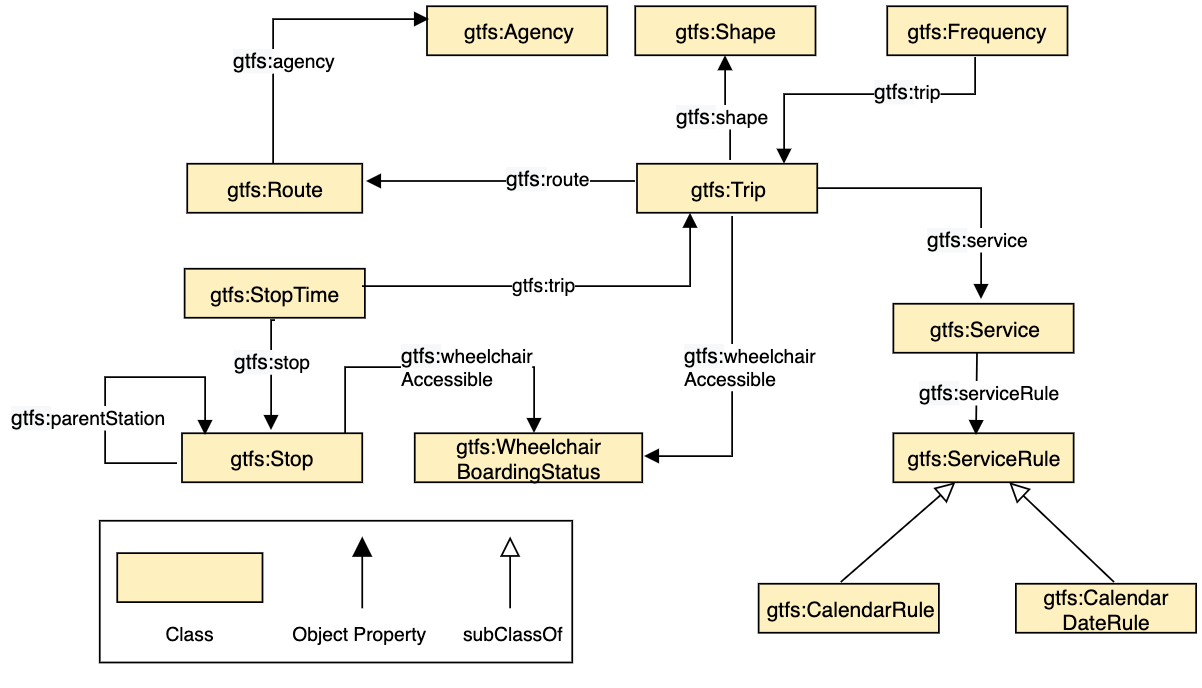
\includegraphics[width=0.8\linewidth]{figures/GTFSontology.png}
    \caption[The LinkedGTFS Ontology]{\textbf{LinkedGTFS Ontology.} Subset of the LinkedGTFS ontology used in the GTFS-Madrid-Bench for virtual knowledge graph access. There are eleven object property relations among the classes, and two subClassOf relations.}
    \label{fig:gtfsOntology}
\end{figure}

\subsubsection{Dataset Generation}

Dataset generation for a virtual knowledge graph access benchmark should be focused on the two main variables that allow testing the capabilities of the engines: (i) data size, and (ii) formats in which data can be expressed. In the context of data generation for OBDA, VIG~\citep{lantivig} proposes the use of R2RML mappings for an efficient scale up of the size of an instance of an RDB dataset. In this case, only one data format (SQL) is involved in the process. 

We use GTFS as the original data source for several reasons: First, GTFS has been the \textit{de-facto} standard for publishing transport data on the web, it also comes with a clear specification, making it easy to understand. Second, the GTFS model comprises several entities that are related through a variety of relationships. In addition it includes different data types such as strings, integers, and booleans. Finally, many cities have adopted the GTFS data model and have published their GTFS data online. Although in our benchmark we propose the use of the GTFS Madrid subway data, GTFS data from a different city could be used as the original data source.

The GTFS-Madrid-Bench proposes an extended workflow using VIG as the Dataset Generator engine for the generation of the datasets taking into account multiple data formats (see an example in Figure \ref{fig:generation}). We describe the detailed steps of the proposed data generation workflow together with examples following the definitions provided in Section \ref{sec:preliminars}:

\begin{enumerate}[label=\textbf{\arabic*})]
    \item \textbf{Data preparation.} The original data source, GTFS, is in CSV format. VIG requires an instance of an RDB and an R2RML mapping for scaling up the data source. We use Morph-CSV\footnote{\url{https://github.com/oeg-upm/morph-csv}}, which takes as inputs a set of spreadsheets in the form of CSV files, their corresponding annotations using CSVW~\citep{tennison2015model} and an RML mapping~\citep{dimou2014rml}. It automatically produces the corresponding schema of an RDB (identifying typical constraints such as datatypes, PK/FK, indexes and NULLs) and an R2RML mapping document, which are the inputs for VIG. 
    
    For the Madrid-GTFS-Bench, we use as input an open data dataset GTFS$_{mad}^{CSV}$ = (GTFS$_{mad}$, GTFS, CSV). GTFS$_{mad}$ is the set of data sources of the subway network of Madrid that has been provided by its transport authority according to the schema GTFS as described in its specification\footnote{\url{https://developers.google.com/transit/gtfs/}}. This dataset is composed of a set of CSV files containing data of Agency, Route, Shape, Frequency, Trip, StopTime, Stop, Calendar and CalendarRule. This input is fixed during all of the data generation process, which means that the generated datasets are defined by the same schema and all of the generated data is obtained from this initial dataset. We create the corresponding RML mapping rules and CSVW metadata annotations and, using the Morph-CSV engine, we generate the corresponding RDB instance GTFS-SQL-1=(GTFS$_{mad}^{SQL}$,1) dataset and the R2RML mapping rules.
    
    \item \textbf{Data creation.} VIG~\citep{lantivig} takes into account the ontology and the set of R2RML mappings to generate each dataset. This engine also receives as input a scale value $s$ that indicates that the size of each table of the database increases $s$ times. The output of VIG is a set of CSV files, one file for each table of the RDB. In this step the dataset GTFS-CSV-s=(GTFS$_{mad}^{CSV}$,s) is generated, where $s$ is the selected scale value.
    
    \item \textbf{Data distribution.} Finally, each dataset generated using VIG is distributed in several formats. We use open source tools to perform this step such as csv2json, from Python CSVKit\footnote{\url{https://csvkit.readthedocs.io/en/1.0.3/scripts/csvjson.html}} and di-csv2xml\footnote{\url{https://github.com/blue-yonder/di-csv2xml}}, depending on the data formats (JSON and XML). We divide the distribution into two categories in order to cover both OBDA and OBDI approaches: 
    
    In the first category, focused on providing support to OBDA techniques, the sources of each dataset are transformed into a single format (e.g., CSV files are transformed into JSON files). The datasets are transformed to the corresponding ones in JSON, XML, SQL and MongoDB obtaining the following datasets: GTFS-F-s$=$(GTFS$_{mad}^{F}$,s) where $s$ is the scale value and F $\in$ $\{$JSON, XML, SQL, MongoDB$\}$. 
    
    In the second category, focused on virtual KGC approaches, the sources of each dataset have to be transformed from the CSV files into multiple formats (e.g. CALENDAR is a JSON document, AGENCY is a XML file, etc.). To distribute the files and based on the GTFS model, the user may select the sources associated to each format and then the benchmark generates the dataset and the corresponding set of mapping rules. 
    
    Additionally, the benchmark provides by default two datasets taking into account the selected formats (JSON, CSV, XML, SQL and MongoDB) where the number of relations (joins) among sources in different formats is minimized or maximized. The formats of the sources in these datasets is also configurable during the generation data process, in order to allow users to analyze the impact of joins over formats with different features. For example, the join selectivity between shapes and trips is different than the join selectivity between routes and agencies, and depending on the formats of each source, the total query execution time of a processor may be impacted. We describe each dataset in more detail:
    \begin{itemize}
        \item Best Dataset: The number of joins among sources in different formats is minimised but ensuring that all of the formats are covered. The aim of this configuration is to study the behavior of the engines when they have to deal with different data sources but where most of the joins are done between sources in the same format. Hence they may delegate their treatment to the underlying data source manager (e.g. MySQL in RDB) and apply common optimisation techniques in query translation approaches~\citep{priyatna2014formalisation}. To meet this requirement and, having 5 possible formats for the data sources, the proposed groups for best dataset are: trips, shapes, calendar and calendar\_dates sources in one group, routes and agency in another, frequencies in the third group, stop and stop\_times in the fourth one and feed\_info in the last one. This composition generates the GTFS$_{mad}^{B}$ dataset. We show a possible example of a best dataset in Figure \ref{fig:best}. 
       
        \item Worst Dataset: The number of joins among sources in different formats is maximised and the five formats are covered. In this distribution, all the possible joins are among sources in different formats. This means that the virtual KGC engine may be enforced to perform the joins after the execution of the translated queries over the original data sources. In the same manner as the best dataset, the groups of sources are: shapes and stops in one group, trips and feed\_info in another, calendar and agency in the third group, routes and stop\_times in the fourth and calendar\_dates and frequencies in the last one. This composition generates the GTFS$_{mad}^{W}$ dataset. We show a possible example of the worst dataset in Figure \ref{fig:worst}. 
    \end{itemize}
   
\end{enumerate}
 

\begin{figure}[h]
    \centering
    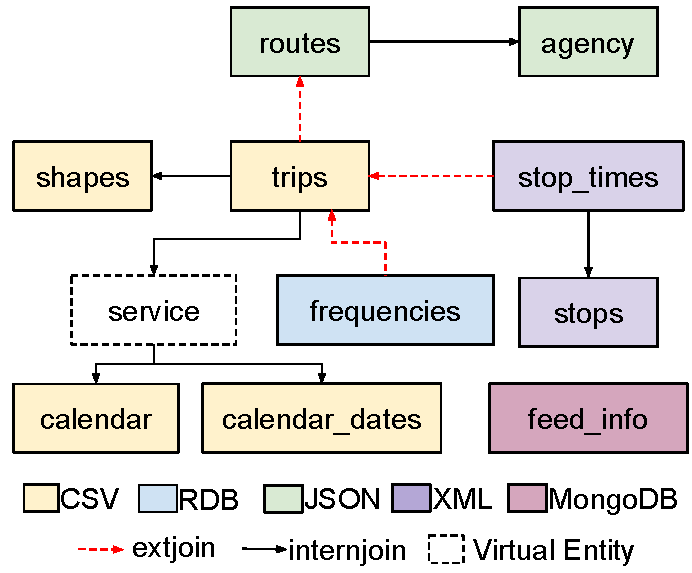
\includegraphics[width=0.85\linewidth]{figures/best-dist.pdf}
    \caption[Example of best dataset]{\textbf{Example of Best Dataset}. Best dataset distributes the formats over the data sources ensuring that at least there is one source per each format and the joins among different formats are minimised. \textit{extjoin} means that there is a relation between sources in different formats and \textit{internjoin} means that the joins are between sources in the same format.}
    \label{fig:best}
\end{figure}


\begin{figure}[h]
    \centering
    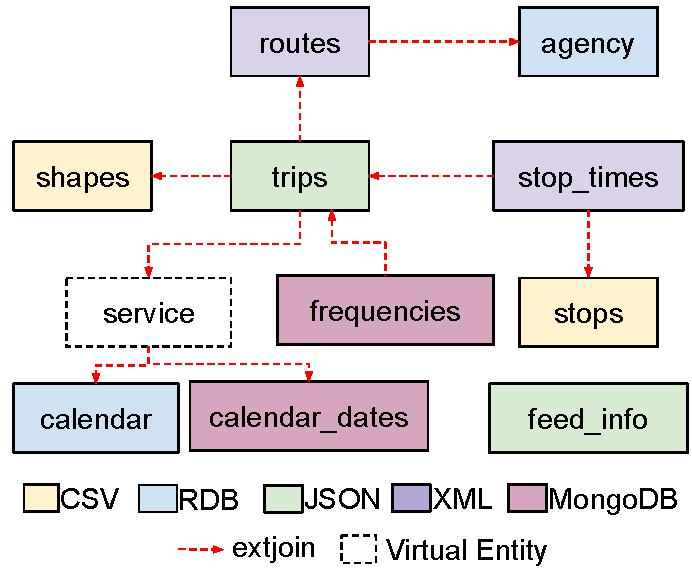
\includegraphics[width=0.85\linewidth]{figures/worst-dist.pdf}
    \caption[Example of worst dataset]{\textbf{Example of Worst Dataset}. Worst dataset distributes the formats over the data sources ensuring that at least there is one source per each format and the joins among different formats are maximised. \textit{extjoin} means that there is a relation between sources in different formats.}
    \label{fig:worst}
\end{figure}

\begin{figure}
    \centering
    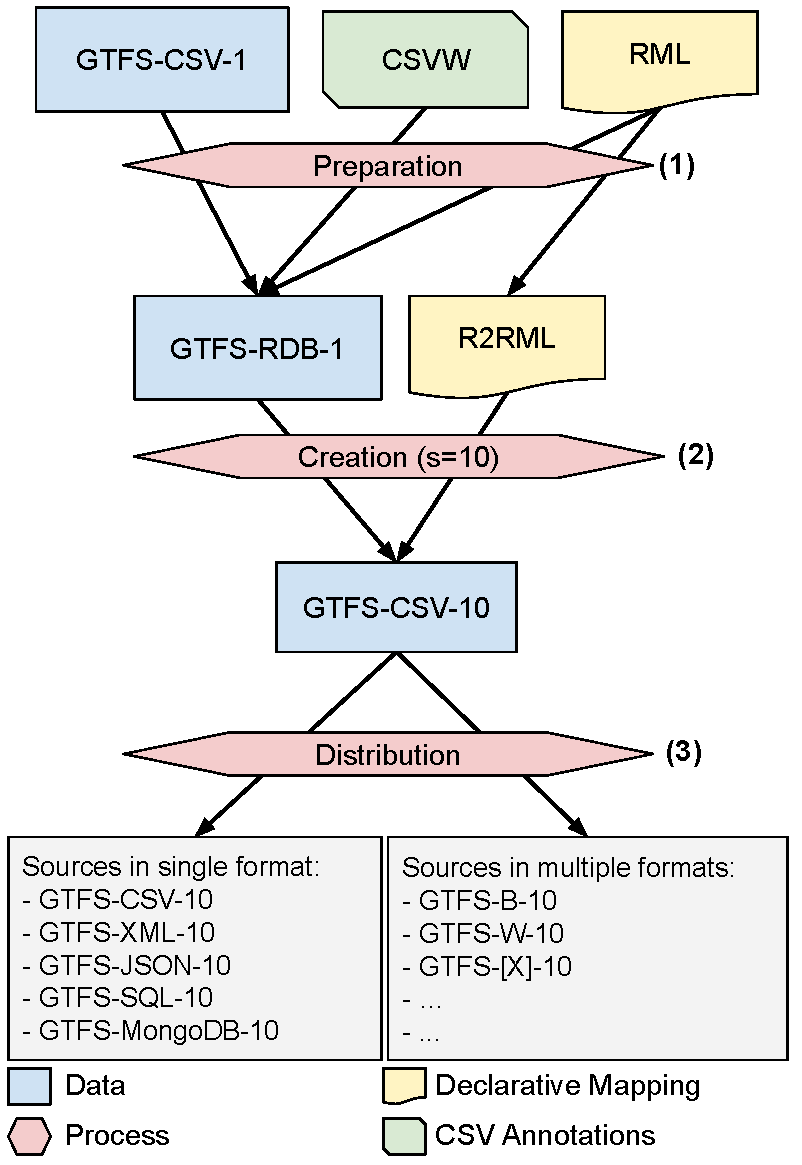
\includegraphics[width=0.7\linewidth]{figures/gprocess.pdf}
    \caption[Generation workflow for scale value 10]{\textbf{GTFS-Madrid-Bench Generation Workflow with scale value 10}. From the original 10 CSV files of Madrid Metro GTFS we use (i) Morph-CSV to generate the corresponding RDB instance and an R2RML mapping that are the required inputs for (ii) scaling up the data using VIG and (iii) distributing the generated CSV dataset to the different formats.}
    \label{fig:generation}
\end{figure}

We want to be able to compare the results obtained by processors with the results obtained by the materialized graph in RDF. For this purpose, we take the output of VIG (e.g., GTFS-CSV-5, GTFS-CSV-10) and we run a materialized KGC process using the SDM-RDFizer\footnote{\url{https://github.com/SDM-TIB/SDM-RDFizer}} engine, which generates the KG in RDF using RML mapping rules. We select this tool because it passed all the RML Test Cases~\citep{heyvaert2019conformance} for CSV files\footnote{\url{http://rml.io/implementation-report/}}, hence we assume that the generation is correct, and that it provides a set of techniques to optimize the generation of RDF at scale. 

\begin{table}[]
\centering
\caption[Mapping features of GTFS]{\textbf{Mapping features of GTFS.} Each TriplesMap of the GTFS mapping file and its corresponding features: the related source, number of Classes, PredicateObjectMaps, Predicates, Objects and RefObjectMaps (joins). }
\label{tab:mappings}
\resizebox{0.9\textwidth}{!}{%
\begin{tabular}{l|l|l|c|c|c|c}
\hline
\multicolumn{1}{c|}{\textbf{TriplesMap}} & \multicolumn{1}{c|} {\textbf{Source}} & {\textbf{Classes}} & \textbf{\#PredicateObjectMap} & \textbf{\#Predicates} & \textbf{\#Objects} & \textbf{\#RefObjectMap} \\ \hline
shapes          &  shapes              & gtfs:Shape                               & 4                     & 4            & 4         & 0      \\ \hline
trips           &  trips              & gtfs:Trip                               & 8                     & 8            & 5         & 4      \\ \hline
calendar\_rules         & calendar              & gtfs:CalendarRule                               & 9                     & 9            & 9         & 0      \\ \hline
calendar\_date\_rules   &  calendar\_dates            & gtfs:CalendarDateRule                               & 2                     & 2            & 2         & 0      \\ \hline
stops              &    stops         & gtfs:Stop                               & 12                    & 12           & 11        & 1      \\ \hline
stoptimes         & stop\_times           & gtfs:StopTime                               & 9                     & 9           & 7         & 2      \\ \hline
routes               &  routes         & gtfs:Route                               & 8                     & 8            & 7         & 1      \\ \hline
agency                & agency          & gtfs:Agency                               & 6                     & 6            & 6         & 0      \\ \hline
frequencies       &  frequencies              & gtfs:Frequency                               & 5                     & 5            & 4         & 1      \\ \hline
feed      &  feed\_info               & gtfs:Feed                               & 6                     & 6            & 6         & 0      \\ \hline
service1 &   calendar           & gtfs:Service                               & 1                     & 1            & 0         & 1      \\ \hline
service2 & calendar\_dates       & gtfs:Service                               & 1                     & 1            & 0         & 1      \\ \hline
\textbf{Total}      &  \multicolumn{1}{c|}{10}    & \multicolumn{1}{c|}{11}                           & 71                     & 71            & 60         & 11      \\ \hline
\end{tabular}%
}

\end{table}

\subsubsection{Mappings} 
Mappings play one of the most important roles in the benchmark since they are the main element used for the query translation process. In the state of the art there are multiple engines and tools that use different mapping languages. We select a set of the most relevant declarative mapping languages in the state of the art and we generate the corresponding mapping rules. In more detail, the GTFS-Madrid-Bench provides:
\begin{itemize}
    \item One R2RML mapping document for accessing SQL datasets.
    \item One xR2RML mapping document for accessing MongoDB datasets.
    \item Seven RML mapping documents\footnote{Provided in RML and YARRRML serializations} for accessing CSV, JSON, XML, SQL, MongoDB, Best and Worst datasets.
    \item One CSVW metadata file to provide annotations for the CSV datasets.
\end{itemize}
Conceptually, all the mappings represent the same relations among the concepts of the ontology and the concepts of the GTFS model, but each one has been developed according to a specification that handles the characteristics of each data format. The mappings are composed by a set of rules representing the relation of one element in the ontology with the corresponding schema element from a source. An overview of the rules within the mappings developed for this benchmark is shown in Table \ref{tab:mappings}. The rules of the mappings are very relevant since they contain many parameters that impact on the performance of the virtual knowledge graph access engines~\citep{chaves2019what}. 

More in detail, each source of the GTFS feed has one associated TriplesMap with a rule to associate the generated entities to the class defined in the ontology, and a set of rules for the object and data properties. Additionally, there is a (virtual) entity, Service, in the data model with no corresponding source, what implies the definition of a set of mapping rules to generate the instances of the corresponding class (\texttt{gtfs:Service}). Following the GTFS specification, the identifier of Service can be found either in calendar or calendar\_dates sources. This means that to be aligned with standard declarative mapping specifications (e.g. RML and R2RML only allow one source per TriplesMap), the mapping document needs to define two TriplesMap, one for calendar (service1) and another for calendar\_dates (service2). This also implies that the trips TriplesMap has one predicate (\texttt{gtfs:service}) with two associated refObjectMaps, where the parentTriplesMap are service1 and service2; this allows generating all \texttt{gtfs:Service} defined in the original data source. Because the instances of \texttt{gtfs:WheelchairBoardingStatus} class are only objects in \texttt{gtfs:Trips} and \texttt{gtfs:Stops} triples, they are generated using the template property in trips and stops TriplesMap. In summary, the mapping contains rules to generate instances of 12 classes, 71 PredicateObjectMaps and Predicates, 60 Objects and 11 RefObjectMaps, covering the main features defined in state-of-the-art mapping specifications for KGC. All of the GTFS mappings are detailed in Appendix \ref{sec:appendix2} using the YARRRML~\citep{Heyvaert2018Declarative} serialisation.

% Queries
\subsubsection{Queries}
Table \ref{tab:queries} presents all the variables considered for the 18 queries in our benchmark. We have developed queries that are based on the Linked GTFS ontology, and are aligned with user stories in Madrid's transport domain, together with different combinations of values for the variables. It should be mentioned that the queries cover all of the data sources that were generated by the Madrid's transport authority as GTFS data from the metro system. These include agencies, routes, stops, trips, frequencies, shapes, calendar, and calendar dates. Although in the benchmark we have defined mappings to translate queries into the underlying query language of the source, these are independent from the queries (we have used these mappings to generate the materialized knowledge graph in the data generation step).

We have defined two sets of 18 queries with identical templates but differences in the constants that appear in subjects or objects of bounded triple patterns: (1) Baseline queries with constants that belong to Madrid's GTFS Linked Data, and (2) VIG queries with constants that belong to the datasets generated by the tool; these queries are executed in the evaluation described in Section \ref{sec:evaluation}. 

\begin{sidewaystable*}[p]
\centering
\caption{GTFS-Madrid-Bench Queries}
\label{tab:queries}
\resizebox{1\textwidth}{!}{%
\begin{tabular}{c|l|c|c|c|c|c|c|c|c|c}
\hline
%Query & Description & \#Triple  & \#Sources & OPTIONAL & Aggregation & Other & FILTER & FILTER & Star-shaped groups  \\ 
Query & Description & \#Triple  & \#Sources & OPTIONAL & Aggregation & Other & \multicolumn{2}{ |c| }{FILTER} & \multicolumn{2}{ |c }{\#Star-shaped groups} \\   
 &  & Patterns  &  & &  & features  & equal to & relational  &  w/o constants & w/constants \\ \hline
q1 & All shapes & 4 & 1 &  &  &  &  &  & 1 & 0 \\ \hline
q2 & All stops where the latitude is larger than a & 5 & 1 & \checkmark &  &  &  & \checkmark & 0 & 1 \\ 
&  specific value &  &  &  &  &  &   &   &  & \\ \hline
q3 & Accessibility information of all stations & 5 & 1 & \checkmark &  &  & \checkmark &  & 0  & 1 \\ \hline
q4 & All agencies and their routes & 9 & 2 & \checkmark &  &  &  &  & 2 & 0 \\ \hline
q5 & Services that have been added after a specific date& 5 & 2 &  &  &  &  & \checkmark & 1 & 1 \\ \hline
%&  specific date  &  &  &  &  &  &   &   &  & \\ \hline
q6 & Number of routes covered by a specific agency & 3 & 2 &  & \checkmark &  & \checkmark &  &  0  & 2 \\ \hline
q7 &  All wheelchair-accessible stops in a specific route   & 15 & 4 & \checkmark &  & DISTINCT & \checkmark &  & 1 & 3 \\ \hline
q8 & Routes and their related trips, services, stops and stop times & 14 & 5 & \checkmark &  &  &  &  & 5 & 0 \\ \hline
q9 &  Trips and associated shapes where latitude  & 7 & 2 & \checkmark &  &  &  & \checkmark & 1 & 1 \\ 
 &  is larger than a specific value &  & &   &  &  &   &  &   &   \\ \hline
q10 &  Number of trips that have a duration   & 4 & 2 &  & \checkmark & DISTINCT &  & \checkmark & 1 & 1 \\ 
 &  over a number of minutes &  &  &  &  &  &   &   &  & \\ \hline
q11 & Trips that are available on a certain date  & 12 & 3 &   &  & NOT EXISTS &  & \checkmark & 3 & 2 \\ \hline
 %&  &  &  &   &  &  &  &  &  & \\ \hline
q12 & Number of stops that are wheelchair-accessible  & 10 & 4 &   & \checkmark & GROUP BY &  &  & 3 & 1 \\ 
 & grouped by route  &  &  &   &  &  &  &  &  & \\ \hline 
q13 & The accesses of all stations & 6 & 1 &  \checkmark &  &  &  &  & 0 & 1 \\ \hline
q14 & All stops times and their related routes and stops ordered by  & 8 & 3  & \checkmark &  & ORDER BY &  &  & 3 & 0 \\ 
  & their sequence, in a specific direction and service  &  &   & &  &  &  &  & & \\ \hline
q15 & For all properties, triples that contain  & 3 & 1 &    &  &  & \checkmark &  & 0 & 1 \\ 
 &  a specific  word in the object placeholder  &  &  &    &  &  &  &  & & \\ \hline
q16 & For all routes, all calendar changes in  & 8 & 3 &    &  &  &  & \checkmark & 2 & 1 \\ 
 &  a specific month &  &  &    &  &  &  &  & & \\ \hline
q17 & Trips with their start and end time  & 9 & 3 &   &  &  &  &  & 3 & 0 \\  
 & of the frequencies and associated routes    &  & &   &  &  &  &  & & \\  \hline
q18 & All routes that have trips on Sunday  & 8 & 5 &   &  & UNION &  &  & 4 & 1 \\ \hline 
\end{tabular}%
}
\end{sidewaystable*}


\subsubsection{Metrics}
In this section we define the metrics that are used to evaluate the performance of Virtual Knowledge Graph access engines. The metrics consider the workflow followed by Virtual Knowledge Graph systems, and for each of the steps identified in the workflow we introduce a set of metrics to be measured and reported.
\begin{table}[]
\caption[Metrics VS dimensions]{Relation between each relevant metric for the Madrid-GTFS-Bench and the dimensions that can impact over that metric. In the Dimension column, Q means query, M mappings and D data.}
\label{tab:dimsensions}
\begin{tabular}{l|c|c}
\hline
\multicolumn{1}{c|}{\textbf{Metric}} & \textbf{Type or Phase} & \textbf{Dimension}  \\ \hline
\multicolumn{3}{c}{General Metrics}                                                 \\ \hline
Total execution time                & General                & D, Q, M \\ \hline
\# answers                            & General                & D, Q, M \\ \hline
Initial delay                         & General                & D, Q, M \\ \hline
Dief@k                                & C. Behaviour           & D, Q, M \\ \hline
Dief@t                                & C. Behaviour           & D, Q, M \\ \hline
\multicolumn{3}{c}{Specific Metrics (Phases)}                                       \\ \hline
Loading time                          & Starting        & Q, M      \\ \hline
Mapping trans. time              & Starting         & M              \\ \hline
\# requests                           & Distribution      & Q              \\ \hline
Source selec. time                 & Distribution      & Q, M     \\ \hline
Query gen. time                 & Distribution      & Q               \\ \hline
Query rewrit. time                  & Rewriting     & Q                \\ \hline
Query trans. time                & Translation    & Q, M       \\ \hline
Query exec. time                  & Execution     & Q, D          \\ \hline
Query aggreg. time                & Finishing         & D                 \\ \hline
\end{tabular}
\end{table}

The workflow extends the OBDA phases identified by Mora and Corcho~\citep{mora2013towards}, and Lanti et al.~\citep{lanti2015npd}. In addition, it includes some of the steps that are defined by proposals that federate queries~\citep{schwarte2011fedx}. General metrics to be captured are \textbf{overall execution time}, \textbf{completeness of answers} and \textbf{initial delay}. Other metrics may be considered when the engine generates answers following a continuous behavior~\citep{sharaf2008algorithms}, such as \textbf{dief@k} or \textbf{dief@t} proposed in \citep{acosta2017diefficiency}. Additionally, for each phase of a workflow, a virtual knowledge graph construction engine may capture specific metrics that allow the identification of bottlenecks in the implementations. This relevant set of metrics for each phase are: (i) \textbf{loading time} during the starting phase when the ontology, mappings and query are loaded; (ii) \textbf{total number of requests} and \textbf{source selection time} during the source selection phase (the engine identifies the sources that can be used to answer the query); (iii) \textbf{query generation time} when the set of sub-queries to be evaluated over each data source is created, and the query plan is generated; (iv) \textbf{mapping translation time} when the engine requires to translate a provided mapping into another one in in a different language, maintaining a set of properties between them~\citep{corcho2019towards}; (v) \textbf{query rewriting time} when the generated sub-queries are rewritten to other queries, taking into account potential inferences from the ontology and information in the mapping~\citep{mora2014kyrie2}; (vi) \textbf{query translation time} when the engine, taking the mapping into account, translates each sub-query to another one in the query language supported by the underlying data sources such as SPARQL-to-SQL~\citep{chebotko2009semantics}; (vii) \textbf{query execution time} when the translated queries are evaluated against the underlying data sources and the results are translated to RDF or as SPARQL bindings using the rules provided in the mappings; and (viii) \textbf{query aggregation time} when the results obtained for each sub-query are aggregated, including the removal of duplicates and the linking of resources. Variables that have an impact on the metrics have been grouped into three dimensions: Query, Data, and Mappings. The relation between each  metric considered  and the dimensions that can impact over that metric is  shown in Table \ref{tab:dimsensions}.

\noindent\paragraph{\textbf{Query.}} The Query dimension variables refer to the structure of the queries, e.g. \#triple patterns, \#sources, and  \#star-shaped groups. A  Star-shaped group is a group of triple patterns that are ``joined" over the same subject or object variable~\citep{vidal2010efficient}. The most common case in real-world scenarios are subject star-shaped groups that represent properties that describe one source. The benchmark considers an increasing number of triple patterns, from 3 to 15, also the number of sources vary from 1 to 5. In particular we have several queries on 1 source with a varying number of triple patterns, and queries that have a large number of triple patterns combined with 4 and 5 sources. With respect to these two variables, our aim is to balance real-life use cases where several properties in the specification need to be combined and retrieved, and query complexity (worst case scenario is the ``Worst Dataset'' when the five sources are represented in the five available formats and the number of joins among sources is maximized).Furthermore, a large number of sources or triple patterns  combined with a large number of non-instantiated star-shaped groups should impact overall execution time and also specifically impact query generation, query rewriting, query translation, and query execution times. 

In general, queries in GTFS-Bench-Madrid combine those that contain single star-shaped groups ($q1$,$q2$, $q3$, $q15$) with those that contain chains of star-shaped groups, that is, where the object of a pattern in a group is the subject in the next group (with joins across different sources): $q4$, $q5$, $q6$, $q7$, $q9$, $q10$, $q11$, $q12$, $q16$, $q17$, $q18$. According to the ontology structure shown in Figure \ref{fig:gtfsOntology}, \texttt{gtfs:StopTime} relates to stops and trips and may lead to hybrid shapes such as $q8$ and $q14$. There is also the case of query $q13$, which refers one source and contains a self-join that relates an access to a station to its ``parent'' station.

Besides, as mentioned in~\citep{montoya2012benchmarking}, query plans generated by query evaluation systems during the subquery generation phase may be affected by the structural properties of a query. If the sources in the dataset are all represented in the same format, then query plans will be generated by the underlying engine (either an RDB engine or a NoSQL engine), and execution time will be affected by the number of joins within star-shaped groups and among these groups. When the sources of the dataset are not in the same format, the engine has to create the query plan. The performance will be affected by the plan proposed by the engine. Different combinations of these variables are considered in GTFS-Madrid-Bench queries: on the one hand we have a large number of triple patterns, sources and star-shaped groups in $q7$ and $q8$, and on the other hand queries like $q18$ combine a large number of sources and star-shaped groups with a medium-sized query (8 triple patterns).

Complexity of SPARQL queries is presented in~\citep{perez2009semantics}, considering the SPARQL fragment with only AND and FILTER operators. Complexity is linear on the product of the dataset size and the size of the query (\# triple patterns), and evaluation is NP-complete for queries constructed with AND, FILTER and UNION operators. Several queries in GTFS-Madrid-Bench have FILTER clauses and specifically, $q18$ contains a UNION of two triple patterns.

The evaluation problem becomes harder when the OPTIONAL operator is added~\citep{perez2009semantics}. Additionally, the work described in~\citep{xiao2018efficient} presents optimization techniques applied in an OBDA setting specifically for queries that have to deal with OPTIONAL triple patterns, claiming that the underlying database systems do not optimize adequately these class of queries. Similar problems may be expected for querying CSV, XML and JSON data sources. We have designed eight queries that use OPTIONAL graph patterns (according to the corresponding non-mandatory attributes in the specification). 

Constants in triple patterns together with FILTER with equality operators increase the selectivity of queries and are likely to reduce the cost of evaluating the query. According to~\citep{montoya2012benchmarking}, instantiated triple patterns have an important impact on the potential number of join intermediate results that may be generated throughout query execution. However, using a FILTER relational operator specially in the case of open ranges, e.g. a FILTER with a $>$ operator, may generate a large number of answers. We have considered several combinations of number of star-shaped groups with and without constants, $q8$ has no constants whereas in $q4$ both star-shaped groups in the query have bindings. An example of an intermediate case occurs in $q12$ with 1 out of 4 instantiated star-shaped groups. 

Three queries contain the aggregated COUNT function, and one of these queries contains additionally the GROUP BY modifier. Other queries use language features like DISTINCT and ORDER, what will impact on the query execution time metric because all of them require an ordering of the tuples/entries of the underlying sources. We cover the impact of these variables in $q7$ and $q10$ with DISTINCT, and $q12$ and $q14$ with GROUP BY and ORDER BY respectively. Finally, having unbounded predicates in a query ($q15$) increases its complexity because the search space during query evaluation may be large. 

The work in~\citep{angles2016negation} studies the impact of negation in the computational complexity of SPARQL queries, it distinguishes four types of negation: negation of filter constraints, negation as failure, negation by MINUS and negation by NOT EXISTS.  The use of NOT EXISTS introduces similar issues to sub-query evaluation because of the  presence of correlated variables and the use of a nested iteration method to evaluate queries that contain this type of negation. Hence $q11$ contains negation with NOT EXISTS.


\noindent\paragraph{\textbf{Mappings.}}
Features of mappings are relevant because they may impact  the performance of the engines. Previous work by~\citep{chaves2019what} evaluates different mapping variables that impact in the construction of a knowledge graph. Similarly, we consider that the following mapping variables influence overall query execution time and specifically query translation and query rewriting times. Regarding structure, we have considered the variables \#Classes, \#PredicateObjectMaps, \#Predicates, \#Objects, and \#RefObjectMap that are presented in Table \ref{tab:mappings}. Another variable is relation type, the mappings of the Madrid-GTFS-Bench include 1-1, 1-N, N-1 and N-M relation types. In general mappings for sources that represent N-M relationships (e.g. stop\_times) are more complex and thus time consuming for query execution. Additionally, the variable \texttt{rr:termtype} of the \texttt{rr:objectMap} may also have an effect because the cost of generating a constant, a reference or a template is not the same.

\noindent\paragraph{\textbf{Dataset.}}
Variables in this dimension include dataset size and the formats of its sources. As already mentioned in Section \ref{sec:datageneration}, datasets with different scale factors are generated in GTFS-Madrid-Bench. Size has an impact on the overall execution time, on the initial delay, and specifically on query execution time because of the larger number of intermediate results. It also influences query aggregation time because in the benchmark, queries against larger datasets generate a larger number of answers.

The format variable may take a single value for datasets in only one format (RDB, CSV, XML, MongoDB, JSON) or multiple formats (Best, Worst and Random). This variable has an impact on the overall execution time, specifically on the query translation and query execution times, as well as on the number of answers because  different formats have different access methods and different underlying query languages.

The work in~\citep{montoya2012benchmarking} presents partitioning and data distribution in this dimension. In GTFS-Bench-Madrid there are fixed values for these variables: the partitioning is vertical and datasets and databases are loaded in local machines.

\subsection{Sustainability and extensibility}
The Madrid-GTFS-Bench is supported by a set of robust resources in order to ensure its sustainability. The benchmark can be adapted to any other virtual knowledge graph access engine that uses other mapping rules languages, or to other non-declarative proposals. The developers or users only have to create the mapping documents according to that specification. Additionally, virtual knowledge graph access engines that work with other graph query languages (e.g. Morph-GraphQL~\citep{priyatna2019morph}) can take advantage of our proposed benchmark. 

A set of improvements for the data generation that we have identified are based on VIG, a robust and efficient engine for the generation of scalable datasets. Additionally, all the generated resources are available online \footnote{\url{https://github.com/oeg-upm/gtfs-bench/}} and their deployment (engines and databases) is done using docker images to ensure the reproducibility of the obtained results. Finally, because we define the dimensions of mappings and datasets taking into account the relevant parameters in the process of constructing knowledge graphs~\citep{chaves2019what}, this benchmark can be also used to test the materialization KGC engines such as RMLMapper~\footnote{\url{https://github.com/RMLio/rmlmapper-java}}, RocketRML~\footnote{\url{https://github.com/semantifyit/RocketRML/}} or SDM-RDFizer~\footnote{\url{https://github.com/SDM-TIB/SDM-RDFizer}} since, at this moment, there is no proposal to evaluate the performance and completeness of these engines in an objective manner.

The possibility to extend this benchmark is also one of the main points that differentiates this proposal to previous ones. First, there are multiple benefits obtained from relying on an open data model from the transport domain, such as linking this data with other data from the city and also having other GTFS transport systems feeds (e.g. metro and train datasets). In addition to queries that take into account the specific characteristics of the selected datasets, it is also possible to incorporate more complex mapping rules with extended features such as specific transformation functions~\citep{de2016ontology}, something that is difficult to address by previous proposals as their data model is usually relational database oriented ~\citep{bizer2009berlin,lanti2015npd}. The incorporation of these features will ensure that we cover new characteristics of the new generation of virtual knowledge graph access engines without the need of creating a benchmark from scratch.  


\subsection{Experimental Evaluation}
In this section we describe the evaluation performed using our benchmark. We first describe the selected virtual KGC engines involved in the evaluation, we describe the evaluation methodology and infrastructure, based on the use of docker images to ensure the reproducibility of the experiments, and finally, we provide the obtained results. All the resources used in this evaluation, such as queries, data, mappings, running scripts, results and docker images for engines and databases are publicly available online\footnote{\url{https://github.com/oeg-upm/gtfs-bench}}.

\subsubsection{Tools}

We selected the most relevant open source virutal KGC engines in the state of the art: 

\noindent\textbf{Ontario.} Ontario~\citep{endris2019ontario}\footnote{\url{https://github.com/SDM-TIB/Ontario}} is an virtual KGC engine from heterogeneous data sources that is based on the concept of RDF molecule templates (RDF-MT)~\citep{endris2017mulder}. Ontario exploits the information provided by the mapping rules for creating the corresponding RDF-MT over the data sources. After the source selection and sub-query generation processes, Ontario translates the SPARQL query into the corresponding query language of the original data source. It supports the following formats: RDF, MySQL, CSV, TSV, JSON, XML, MongoDB and Neo4j.

\noindent\textbf{Ontop.} Ontop~\citep{rodriguez2015efficient}\footnote{\url{https://github.com/ontop/ontop}} is an KGC system from RDB instances that includes both materialization and virtualization techniques. Ontop translates R2RML mappings into its own mapping language, called ``OBDA mappings''. These mappings, and a SPARQL query if available, are transformed into datalog rules, allowing semantic optimization techniques to be applied, and generating efficient SQL queries (e.g., self-join elimination). It only supports the SQL format.

\noindent\textbf{Morph-RDB.} Morph-RDB~\citep{priyatna2014formalisation}\footnote{\url{https://github.com/oeg-upm/morph-rdb}} is an R2RML engine that also includes materialization and virtualization techniques. The formalization of its query translation technique is based on the R2RML-based extension of SPARQL-to-SQL query translation algorithm proposed by~\citep{chebotko2009semantics}, originally designed to work with RDB-backed triples store. Similar to Ontop, several optimization techniques are also incorporated in order to generate more efficient SQL queries. It supports SQL and CSV files.

\noindent\textbf{Morph-xR2RML.} Morph-xR2RML~\citep{michel2015translation}\footnote{\url{https://github.com/frmichel/morph-xr2rml}} uses the xR2RML mapping language to support the generation of RDF lists, and to query data stored in NoSQL databases such as MongoDB.

\noindent\textbf{Morph-CSV.} Morph-CSV~\citep{chaves2020enhancing}\footnote{\url{https://github.com/oeg-upm/morph-csv-sparql}} exploits the information of CSVW annotations and RML mappings to enforce implicit constraints over tabular data, explicitly declared in these annotations. It can be integrated on top of any existing SPARQL-to-SQL engine in order to enhance query completeness and performance.

We also intended to include other engines such as Squerall~\citep{mami2019querying} or Polyweb~\citep{khan2019one}. In both cases, either the code is not available as open source or it was not feasible to run the engine due to the lack of documentation. Issues have been reported in their corresponding repositories, with the intention of alerting the authors and maintainers about the current limitations.

\subsubsection{Setup}
In this section we describe how we use our benchmark to evaluate several processors/engines that have been described in Section \ref{sec:tools}. 

We have setup several experiment configurations for evaluating the selected processors. As an example, the experiment configurations for query $q4$ can be seen in Table \ref{tab:ExperimentalEnvironment}. These experiment configurations have a fixed set of mappings with routes and agencies. The processor used to evaluate this query depends on the dataset, for example, Ontario in the case of the JSON dataset or Morph-RDB, Ontario and Ontop for SQL.

\begin{table}[]
\centering
\caption[Experiment configuration example set]{\textbf{Experiment configuration example set.} List of experimental configurations and processors for q4. $D$ is a dataset where $s$ is the scaling factor (i.e., 1, 5, 10, 50, 100, 500), $M$ is the set of mappings, $q$ is the SPARQL query, $\phi$ is a processor. $q$ is a SPARQL query defined in the Appendix Section.}
\label{tab:ExperimentalEnvironment}
\resizebox{0.8\textwidth}{!}{%
\begin{tabular}{c|c|c|c}
\hline
\textbf{Query $q$} & \textbf{Dataset $D$} & \textbf{TriplesMap $M$} & \textbf{Processor $\phi$} \\ \hline
\multirow{11}{*}{q4} & \multirow{3}{*}{GTFS$_{mad}$-CSV-s} & \{routes,agency\}$_{RML}$ & Morph-CSV \\ \cline{3-4} 
 &  & \{routes,agency\}$_{R2RML}$ & Morph-RDB \\ \cline{3-4} 
 &  & \{routes,agency\}$_{RML}$ & Ontario \\ \cline{2-4} 
 & \multirow{3}{*}{GTFS$_{mad}$-SQL-s} & \{routes,agency\}$_{R2RML}$ & Morph-RDB \\ \cline{3-4} 
 &  & \{routes,agency\}$_{RML}$ & Ontario \\ \cline{3-4} 
 &  & \{routes,agency\}$_{OBDA}$ & Ontop \\ \cline{2-4} 
 & GTFS$_{mad}$-MongoDB-s & \{routes,agency\}$_{xR2RML}$ & Morph-xR2RML \\ \cline{2-4} 
 & GTFS$_{mad}$-XML-s-s & \{routes,agency\}$_{RML}$ & Ontario \\ \cline{2-4} 
 & GTFS$_{mad}$-JSON-s & \{routes,agency\}$_{RML}$ & Ontario \\ \cline{2-4} 
 & GTFS$_{mad}$-B-s & \{routes,agency\}$_{RML}$ & Ontario \\ \cline{2-4} 
 & GTFS$_{mad}$-W-s & \{routes,agency\}$_{RML}$ & Ontario \\ \hline
\end{tabular}%
}
\end{table}


All the experiment configurations are loaded into a machine with the following characteristics: 2GHz CPU with 15 cores, 32 RAM, 200 GB HDD with Ubuntu 18.04 as its operating system. The machine contains a docker image for each of the processors: Morph-RDB v3.12.5, Ontop v3.0.0, Morph-CSV v1.0.0, Ontario v.0.3, Morph-xR2RML-1.1-RC2. All the engines are configured with the recommended settings provided in the corresponding online repository. 

In terms of data size, we decide to evaluate the engines over the scale values (5, 10, 50, 100 and 500). After some preliminary tests, we observed that these values provide a good overview of the current state of the engines in terms of query evaluation performance. For each SQL dataset size, we create two docker images where the data is loaded, one as an instance of the MySQL Database Server v5.5 and another as an instance of the MySQL Community Server v8.0. Similarly, for each MongoDB dataset size, we create a docker image of an instance of the MongoDB Community Server v3.4 with the dataset is loaded. The rest of the datasets, which correspond to raw data (CSV, XML and JSON), are loaded into the machine and are accessible to all the processors. 

In the case of Morph-RDB, we use it together with the docker images containing the instances of the MySQL Community Server v5.5, according to the corresponding documentation. As for Morph-xR2RML, we use it together with the docker images containing the instances of MongoDB server version v3.4. For these experimental configuration and processors, we evaluate all the 18 queries both in warm and in cold mode. Each query is run five times. In warm mode we want to analyze how the cache mechanism may affect the performance. In order to do so, we first evaluate the query, discard its result and then run  the query again five times, we then compute the average query execution time. On the contrary, in  cold mode, we want to study the performance of the processors without the effect of the cache. In order to do so, we run the query five times and we always restart the database server after each run, so as to clean all the caches. %from the database server. 

Additionally, we use Ontario and Ontop with the docker images containing the instances of MySQL server v8.0, the latest version at the time of writing. Note that the use of cache is not supported anymore in MySQL v8.0 so that we only evaluate our queries in cold mode. We perform the rest of the experiment configurations with Ontario against the CSV and JSON datasets, and Morph-CSV against CSV datasets. 

\begin{table}[]
\caption[Overall execution time GTFS-1]{Overall execution time (in seconds) of  benchmark queries in experiment configurations with original size datasets. W means that the engine obtained a different number of results in comparison to the baseline. E means that the processor is not able to execute the query. TO means that the processor is not able to evaluate the query within the timeout duration (3600 seconds).}
\label{tab:gtfs1}
\resizebox{\textwidth}{!}{%
\begin{tabular}{|l|l|l|l|l|l|l|l|l|l|l|l|l|l|l|l|l|l|l|l|l|}
\hline
\multicolumn{1}{|c|}{\multirow{2}{*}{\textbf{Dataset}}} & \multicolumn{2}{c|}{\textbf{Processor}} & \multicolumn{18}{c|}{\textbf{Query}}                                                                                                                                                                                                                               \\ \cline{2-21} 
\multicolumn{1}{|c|}{}                                  & \textbf{Cache}         & \textbf{Name}  & \textbf{q1} & \textbf{q2} & \textbf{q3} & \textbf{q4} & \textbf{q5} & \textbf{q6} & \textbf{q7} & \textbf{q8} & \textbf{q9} & \textbf{q10} & \textbf{q11} & \textbf{q12} & \textbf{q13} & \textbf{q14} & \textbf{q15} & \textbf{q16} & \textbf{q17} & \textbf{q18} \\ \hline
\multirow{4}{*}{GTFS-SQL-1}                             & Warm                   & Morph-RDB      & 5.85        & 2.07        & E           & 1.82        & W           & 1.86        & 1.97        & E           & 26.02       & 1.80         & E            & 1.81         & 2.06         & W            & 1.89         & E            & 2.11         & E            \\ \cline{2-21} 
                                                        & \multirow{3}{*}{Cold}  & Ontario        & 18.02       & E           & TO          & E           & E           & E           & E           & W           & E           & E            & E            & E            & E            & W            & E            & E            & E            & E            \\ \cline{3-21} 
                                                        &                        & Morph-RDB      & 7.14        & 2.65        & E           & 2.42        & W           & 2.36        & 2.43        & E           & 28.65       & 2.38         & E            & 2.41         & 2.69         & W            & 2.58         & E            & 2.68         & E            \\ \cline{3-21} 
                                                        &                        & Ontop          & 8.37        & 5.04        & 5.18        & E           & W           & E           & W           & E           & 16.56       & E            & E            & E            & 5.06         & W            & 5.10         & W            & 5.00         & E            \\ \hline
\multirow{2}{*}{GTFS-MongoDB-1}                         & Warm                   & Morph-xR2RML   & W           & W           & W           & W           & W           & W           & W           & W           & W           & W            & W            & W            & W            & 28.67        & W            & W            & 6.52         & W            \\ \cline{2-21} 
                                                        & Cold                   & Morph-xR2RML   & W           & W           & W           & W           & W           & W           & W           & W           & W           & W            & W            & W            & W            & 28.17        & W            & W            & 6.96         & W            \\ \hline
\multirow{3}{*}{GTFS-CSV-1}                             & \multirow{3}{*}{Cold}  & Morph-RDB      & 6.94        & 3.04        & E           & 2.78        & E           & 2.78        & TO          & E           & TO          & 2.97         & E            & 6.23         & 3.97         & E            & E            & E            & 3.14         & E            \\ \cline{3-21} 
                                                        &                        & Morph-CSV      & 15.11       & 10.88       & E           & 10.72       & E           & 9.95        & 10.84       & E           & 40.90       & 10.70        & E            & 11.60        & 11.82        & E            & E            & E            & 11.48        & W            \\ \cline{3-21} 
                                                        &                        & Ontario        & W           & E           & 17.34       & E           & E           & E           & E           & W           & E           & E            & E            & E            & E            & W            & E            & E            & E            & E            \\ \hline
GTFS-XML-1                                              & Cold                   & Ontario        & E           & E           & E           & E           & E           & E           & E           & E           & E           & E            & E            & E            & E            & E            & E            & E            & E            & E            \\ \hline
GTFS-JSON-1                                             & Cold                   & Ontario        & 18.04       & E           & 17.14       & E           & E           & E           & E           & W           & E           & E            & E            & E            & E            & W            & E            & E            & E            & E            \\ \hline
GTFS-B-1                                                & Cold                   & Ontario        & W           & E           & 17.14       & E           & E           & E           & E           & W           & E           & E            & E            & E            & E            & W            & E            & E            & E            & E            \\ \hline
GTFS-W-1                                                & Cold                   & Ontario        & W           & E           & 17.14       & E           & E           & E           & E           & W           & E           & E            & E            & E            & E            & W            & E            & E            & E            & E            \\  \hline
\end{tabular}%
}
\end{table}

\subsubsection{Results}
In this section we report the results obtained through our experimental configurations. Table \ref{tab:gtfs1} presents the results obtained for all of the datasets and all the processors with scale 1 and a timeout of 3600s (1 hour). The rest of the Tables (\ref{tab:gtfs5},\ref{tab:gtfs10},\ref{tab:gtfs50},\ref{tab:gtfs100},\ref{tab:gtfs500}) report the results for the other scale values (5, 10, 50, 100 and 500) with the same timeout. When an engine reports an error (e.g. a SPARQL query parsing error, memory overhead, etc) we represent it with an \texttt{E} in the table. When the engine does not report any error but the number of results obtained differs with respect to the baseline (RDF materialised graph), we represent the cell with a \texttt{W}. We do not report the total execution time of those queries because in general these cases report 0 results in the execution but without error, so the time is not relevant. The tables comparing the number of results obtained by the baseline and the evaluated engines is reported in Annex \ref{sec:appendix3}.  

In terms of the comparison among different data formats, we can observe that CSV and SQL data formats are the ones best supported by the available engines. In these cases, most of the engines are able to answer a significant number of  queries.
As to the effect of cache, as it is expected, evaluation in the warm mode needed less time, yet, the difference is insignificant due to the relatively small size of the datasets. 

We can also see that in general, it takes more time to evaluate queries over CSV datasets than over SQL datasets. This is expected because available engines need to first load the CSV dataset in a SQL database server in order to be able to query the dataset.

This is not the case of other data formats such as JSON and MongoDB, where the engines are only able to answer one or two queries. This is even worse in the case of the XML format, where the only engine that supports it is not able to answer any query. Similarly in the distributed format, the only query that can be answered by the virtual KGC engine is a query that is evaluated against a JSON dataset.

This trend holds in the other scale factors up to 100. In the scale factor 500, only those engines that use SQL datasets are able to answer queries.

Analysing the results in general, the errors obtained in the execution of the queries (\texttt{E} in the tables) over the tested engines may be due to two main reasons: (i) the engine does not support a SPARQL operator in the original query (ii) the engine is not able to manage large (intermediate) results, for example, maintaining them in memory. Additionally, the differences obtained in terms of query completeness (\texttt{W} in the tables) may be due because: (i) the engine supports the SPARQL operator but it does not translate it correctly to an operator of the underlying database, hence, the query is executed but the number of results obtained are different; (ii) the interpretation of the mapping rules is not performing correctly, hence, the semantics of the original query is not preserved in the translated query.




\begin{table}[]
\caption[Overall execution time GTFS-5]{Overall execution time (in seconds) of  benchmark queries in experiment configurations with size 5 datasets. W means that the engine obtained a different number of results in comparison to the baseline. E means that the processor is not able to execute the query. TO means that the processor is not able to evaluate the query within the timeout duration (3600 seconds).}
\label{tab:gtfs5}
\resizebox{\textwidth}{!}{%
\begin{tabular}{|c|l|l|l|l|l|l|l|l|l|l|l|l|l|l|l|l|l|l|l|l|}
\hline
\multirow{2}{*}{\textbf{Dataset}} & \multicolumn{2}{c|}{\textbf{Processor}}                                  & \multicolumn{18}{c|}{\textbf{Query}}                                                                                                                                                                                                                               \\ \cline{2-21} 
                                  & \multicolumn{1}{c|}{\textbf{Cache}} & \multicolumn{1}{c|}{\textbf{Name}} & \textbf{q1} & \textbf{q2} & \textbf{q3} & \textbf{q4} & \textbf{q5} & \textbf{q6} & \textbf{q7} & \textbf{q8} & \textbf{q9} & \textbf{q10} & \textbf{q11} & \textbf{q12} & \textbf{q13} & \textbf{q14} & \textbf{q15} & \textbf{q16} & \textbf{q17} & \textbf{q18} \\ \hline
\multirow{4}{*}{GTFS-SQL-5}       & Warm                                & Morph-RDB                          & 12.65       & 2.47        & E           & 1.89        & 2.06        & 1.78        & 1.93        & E           & E           & 1.74         & E            & 1.88         & 2.14         & 4.58         & 2.88         & E            & 2.61         & E            \\ \cline{2-21} 
                                  & \multirow{3}{*}{Cold}               & Ontario                            & 117.00      & E           & TO          & E           & E           & E           & E           & W           & E           & E            & E            & E            & E            & W            & E            & E            & E            & E            \\ \cline{3-21} 
                                  &                                     & Morph-RDB                          & 15.14       & 3.24        & E           & 2.40        & 2.71        & 2.34        & 2.62        & E           & E           & 2.41         & E            & 2.70         & 2.82         & 5.59         & 3.89         & E            & 3.39         & E            \\ \cline{3-21} 
                                  &                                     & Ontop                              & 13.87       & 5.40        & 5.31        & E           & W           & E           & W           & E           & W           & E            & E            & E            & 5.24         & 6.61         & W            & W            & 5.37         & E         \\ \hline
\multirow{2}{*}{GTFS-MongoDB-5}   & Warm                                & Morph-xR2RML                       & W           & W           & W           & W           & W           & W           & W           & W           & W           & W            & W            & W            & W            & TO            & W            & W            & TO            & W            \\ \cline{2-21} 
                                  & Cold                                & Morph-xR2RML                       & W           & W           & W           & W           & W           & W           & W           & W           & W           & W            & W            & W            & W            & TO            & W            & W            & TO            & W            \\ \hline
\multirow{3}{*}{GTFS-CSV-5}       & \multirow{3}{*}{Cold}               & Morph-RDB                          & 14.42       & 4.38        & E           & 3.81        & E           & 3.64        & TO          & E           & TO          & 6.57         & E            & TO           & 12.45        & E            & E            & E            & 9.25         & E            \\ \cline{3-21} 
                                  &                                     & Morph-CSV                          & 43.41       & W           & E           & 33.51       & E           & 34.44       & W           & E           & TO          & 33.86        & E            & 36.08        & 34.90        & E            & E            & E            & 35.26        & E           \\ \cline{3-21} 
                                  &                                     & Ontario                            & W           & E           & 18.34       & E           & E           & E           & E           & W           & E           & E            & E            & E            & E            & W            & E            & E            & E            & E            \\ \hline
\multicolumn{1}{|l|}{GTFS-XML-5}  & Cold                                & Ontario                            & E           & E           & E           & E           & E           & E           & E           & E           & E           & E            & E            & E            & E            & E            & E            & E            & E            & E            \\ \hline
\multicolumn{1}{|l|}{GTFS-JSON-5} & Cold                                & Ontario                            & W           & E           & 15.66       & E           & E           & E           & E           & W           & E           & E            & E            & E            & E            & W            & E            & E            & E            & E            \\ \hline
\multicolumn{1}{|l|}{GTFS-B-5}    & Cold                                & Ontario                            & W           & E           & 15.66       & E           & E           & E           & E           & W           & E           & E            & E            & E            & E            & W            & E            & E            & E            & E            \\ \hline
\multicolumn{1}{|l|}{GTFS-W-5}    & Cold                                & Ontario                            & W           & E           & 15.66       & E           & E           & E           & E           & W           & E           & E            & E            & E            & E            & W            & E            & E            & E            & E            \\ \hline
\end{tabular}%
}
\end{table}

\begin{table}[]
\caption[Overall execution time GTFS-10]{Overall execution time (in seconds) of  benchmark queries in experiment configurations with size 10 datasets. W means that the engine obtained a different number of results in comparison to the baseline. E means that the processor is not able to execute the query. TO means that the processor is not able to evaluate the query within the timeout duration (3600 seconds).}
\label{tab:gtfs10}
\resizebox{\textwidth}{!}{%
\begin{tabular}{|l|l|l|l|l|l|l|l|l|l|l|l|l|l|l|l|l|l|l|l|l|}
\hline
\multicolumn{1}{|c|}{\multirow{2}{*}{\textbf{Dataset}}} & \multicolumn{2}{c|}{\textbf{Processor}} & \multicolumn{18}{c|}{\textbf{Query}}                                                                                                                                                                                                                               \\ \cline{2-21} 
\multicolumn{1}{|c|}{}                                  & \textbf{Cache}         & \textbf{Name}  & \textbf{q1} & \textbf{q2} & \textbf{q3} & \textbf{q4} & \textbf{q5} & \textbf{q6} & \textbf{q7} & \textbf{q8} & \textbf{q9} & \textbf{q10} & \textbf{q11} & \textbf{q12} & \textbf{q13} & \textbf{q14} & \textbf{q15} & \textbf{q16} & \textbf{q17} & \textbf{q18} \\ \hline
\multicolumn{1}{|c|}{\multirow{4}{*}{GTFS-SQL-10}}      & Warm                   & Morph-RDB      & 23.78       & 2.88        & E           & 1.93        & W           & 1.75        & 1.97        & E           & E           & 1.85         & E            & 1.94         & 2.46         & 6.61         & 3.46         & E            & 3.07         & E            \\ \cline{2-21} 
\multicolumn{1}{|c|}{}                                  & \multirow{3}{*}{Cold}  & Ontario        & 415.60      & E           & TO          & E           & E           & E           & E           & W           & E           & E            & E            & E            & E            & W            & E            & E            & E            & E            \\ \cline{3-21} 
\multicolumn{1}{|c|}{}                                  &                        & Morph-RDB      & 27.25       & 3.72        & E           & 2.54        & W           & 2.36        & 2.55        & E           & E           & 2.38         & E            & 2.50         & 3.22         & 8.16         & 4.48         & E            & 3.77         & E            \\ \cline{3-21} 
\multicolumn{1}{|c|}{}                                  &                        & Ontop          & 24.05       & 5.56        & 5.57        & E           & W           & E           & W           & E           & W           & E            & E            & E            & 5.29         & 7.58         & W            & W            & 5.62         & E            \\ \hline
\multirow{2}{*}{GTFS-MongoDB-10}                        & Warm                   & Morph-xR2RML   & W           & W           & W           & W           & W           & W           & W           & W           & W           & W            & W            & W            & W            &  TO            & W            & W            &    TO          & W            \\ \cline{2-21} 
                                                        & Cold                   & Morph-xR2RML   & W           & W           & W           & W           & W           & W           & W           & W           & W           & W            & W            & W            & W            &  TO             & W            & W            &   TO           & W            \\ \hline
\multirow{3}{*}{GTFS-CSV-10}                            & \multirow{3}{*}{Cold}  & Morph-RDB      & 25.90       & 6.06        & E           & 5.20        & E           & 4.89        & TO          & E           & TO          & 16.06        & E            & TO           & 38.15        & E            & E            & E            & 38.90        & E            \\ \cline{3-21} 
                                                        &                        & Morph-CSV      & 97.00       & W           & E           & 69.39       & E           & 68.78       & W           & E           & TO          & 69.28        & E            & 71.01        & 68.79        & E            & E            & E            & 72.29        & W            \\ \cline{3-21} 
                                                        &                        & Ontario        & W           & E           & 19.51       & E           & E           & E           & E           & W           & E           & E            & E            & E            & E            & W            & E            & E            & E            & E            \\ \hline
GTFS-XML-10                                             & Cold                   & Ontario        & E           & E           & E           & E           & E           & E           & E           & E           & E           & E            & E            & E            & E            & E            & E            & E            & E            & E            \\ \hline
GTFS-JSON-10                                            & Cold                   & Ontario        & W           & E           & 17.21       & E           & E           & E           & E           & W           & E           & E            & E            & E            & E            & W            & E            & E            & E            & E            \\ \hline
GTFS-B-10                                               & Cold                   & Ontario        & W           & E           & 17.21       & E           & E           & E           & E           & W           & E           & E            & E            & E            & E            & W            & E            & E            & E            & E            \\ \hline
GTFS-W-10                                               & Cold                   & Ontario        & W           & E           & 17.21       & E           & E           & E           & E           & W           & E           & E            & E            & E            & E            & W            & E            & E            & E            & E            \\ \hline
\end{tabular}%
}
\end{table}


\begin{table}[]
\caption[Overall execution time GTFS-50]{Overall execution time (in seconds) of  benchmark queries in experiment configurations with size 50 datasets. W means that the engine obtained a different number of results in comparison to the baseline. E means that the processor is not able to execute the query. TO means that the processor is not able to evaluate the query within the timeout duration (3600 seconds).}
\label{tab:gtfs50}
\resizebox{\textwidth}{!}{%
\begin{tabular}{|l|l|l|l|l|l|l|l|l|l|l|l|l|l|l|l|l|l|l|l|l|}
\hline
\multicolumn{1}{|c|}{\multirow{2}{*}{\textbf{Dataset}}} & \multicolumn{2}{c|}{\textbf{Processor}} & \multicolumn{18}{c|}{\textbf{Query}}                                                                                                                                                                                                                               \\ \cline{2-21} 
\multicolumn{1}{|c|}{}                                  & \textbf{Cache}         & \textbf{Name}  & \textbf{q1} & \textbf{q2} & \textbf{q3} & \textbf{q4} & \textbf{q5} & \textbf{q6} & \textbf{q7} & \textbf{q8} & \textbf{q9} & \textbf{q10} & \textbf{q11} & \textbf{q12} & \textbf{q13} & \textbf{q14} & \textbf{q15} & \textbf{q16} & \textbf{q17} & \textbf{q18} \\ \hline
\multirow{4}{*}{GTFS-SQL-50}                            & Warm                   & Morph-RDB      & 108.42      & 4.91        & E           & 2.08        & W           & 1.75        & 1.97        & E           & E           & 1.89         & E            & 2.29         & 3.69         & 22.55        & 8.27         & E            & 5.56         & E            \\ \cline{2-21} 
                                                        & \multirow{3}{*}{Cold}  & Ontario        & TO          & E           & TO          & E           & E           & E           & E           & W           & E           & E            & E            & E            & E            & W            & E            & E            & W            & E            \\ \cline{3-21} 
                                                        &                        & Morph-RDB      & 121.31      & 6.01        & E           & 2.68        & W           & 2.31        & 2.63        & E           & E           & 2.59         & E            & 2.91         & 4.54         & 27.02        & 10.00        & E            & 6.89         & E            \\ \cline{3-21} 
                                                        &                        & Ontop          & 119.89      & 6.92        & 6.61        & E           & W           & E           & W           & E           & W           & E            & E            & E            & 6.05         & 15.69        & W            & W            & 7.31         & E            \\ \hline
\multirow{2}{*}{GTFS-MongoDB-50}                        & Warm                   & Morph-xR2RML   & W           & W           & W           & W           & W           & W           & W           & W           & W           & W            & W            & W            & W            & TO           & W            & W            & TO           & W            \\ \cline{2-21} 
                                                        & Cold                   & Morph-xR2RML   & W           & W           & W           & W           & W           & W           & W           & W           & W           & W            & W            & W            & W            & TO           & W            & W            & TO           & W            \\ \hline
\multirow{3}{*}{GTFS-CSV-50}                            & \multirow{3}{*}{Cold}  & Morph-RDB      & 128.40      & 22.17       & E           & 19.85       & E           & 19.60       & TO          & E           & TO          & 351.23       & E            & TO           & 1,039.29     & E            & E            & E            & TO           & E            \\ \cline{3-21} 
                                                        &                        & Morph-CSV      & 575.15      & 449.54      & E           & 442.60      & E           & 436.06      & W           & E           & TO          & 444.84       & E            & 443.12       & 447.74       & E            & E            & E            & 443.47       & W            \\ \cline{3-21} 
                                                        &                        & Ontario        & W           & E           & 35.16       & E           & E           & E           & E           & W           & E           & E            & E            & E            & E            & W            & E            & E            & E            & E            \\ \hline
GTFS-XML-50                                             & Cold                   & Ontario        & E           & E           & E           & E           & E           & E           & E           & E           & E           & E            & E            & E            & E            & E            & E            & E            & E            & E            \\ \hline
GTFS-JSON-50                                            & Cold                   & Ontario        & W           & E           & 23.74       & E           & E           & E           & E           & W           & E           & E            & E            & E            & E            & W            & E            & E            & E            & E            \\ \hline
GTFS-B-50                                               & Cold                   & Ontario        & W           & E           & 23.74       & E           & E           & E           & E           & W           & E           & E            & E            & E            & E            & W            & E            & E            & E            & E            \\ \hline
GTFS-W-50                                               & Cold                   & Ontario        & W           & E           & 23.74       & E           & E           & E           & E           & W           & E           & E            & E            & E            & E            & W            & E            & E            & E            & E            \\ \hline
\end{tabular}%
}
\end{table}


\begin{table}[]
\caption[Overall execution time GTFS-100]{Overall execution time (in seconds) of  benchmark queries in experiment configurations with size 100 datasets. W means that the engine obtained a different number of results in comparison to the baseline. E means that the processor is not able to execute the query. TO means that the processor is not able to evaluate the query within the timeout duration (3600 seconds).}
\label{tab:gtfs100}
\resizebox{\textwidth}{!}{%
\begin{tabular}{|l|l|l|l|l|l|l|l|l|l|l|l|l|l|l|l|l|l|l|l|l|}
\hline
\multicolumn{1}{|c|}{\multirow{2}{*}{\textbf{Dataset}}} & \multicolumn{2}{c|}{\textbf{Processor}} & \multicolumn{18}{c|}{\textbf{Query}}                                                                                                                                                                                                                               \\ \cline{2-21} 
\multicolumn{1}{|c|}{}                                  & \textbf{Cache}         & \textbf{Name}  & \textbf{q1} & \textbf{q2} & \textbf{q3} & \textbf{q4} & \textbf{q5} & \textbf{q6} & \textbf{q7} & \textbf{q8} & \textbf{q9} & \textbf{q10} & \textbf{q11} & \textbf{q12} & \textbf{q13} & \textbf{q14} & \textbf{q15} & \textbf{q16} & \textbf{q17} & \textbf{q18} \\ \hline
\multirow{4}{*}{GTFS-SQL-100}                           & Warm                   & Morph-RDB      & 221.11      & 7.48        & E           & 2.30        & W           & 1.75        & 1.96        & E           & E           & 1.99         & E            & 2.65         & 4.68         & 42.44        & 15.51        & E            & 8.54         & E            \\ \cline{2-21} 
                                                        & \multirow{3}{*}{Cold}  & Ontario        & TO          & E           & TO          & E           & E           & E           & E           & W           & E           & E            & E            & E            & E            & W            & E            & E            & E            & E            \\ \cline{3-21} 
                                                        &                        & Morph-RDB      & 245.98      & 8.83        & E           & 3.05        & W           & 2.33        & 2.52        & E           & E           & 2.63         & E            & 3.38         & 5.76         & 50.99        & 19.45        & E            & 10.38        & E            \\ \cline{3-21} 
                                                        &                        & Ontop          & 1,477.38    & 8.87        & 8.25        & E           & W           & E           & W           & E           & W           & E            & E            & E            & 6.80         & 27.18        & W            & W            & 9.20         & E        \\ \hline
\multirow{2}{*}{GTFS-MongoDB-100}                       & Warm                   & Morph-xR2RML   & W           & W           & W           & W           & W           & W           & W           & W           & W           & W            & W            & W            & W            & TO           & W            & W            & TO           & W            \\ \cline{2-21} 
                                                        & Cold                   & Morph-xR2RML   & W           & W           & W           & W           & W           & W           & W           & W           & W           & W            & W            & W            & W            & TO           & W            & W            & TO           & W            \\ \hline
\multirow{3}{*}{GTFS-CSV-100}                           & \multirow{3}{*}{Cold}  & Morph-RDB      & E           & 43.59       & E           & 38.52       & E           & 38.43       & TO          & E           & TO          & 1582.52      & E            & TO           & TO           & E            & E            & E            & TO           & E            \\ \cline{3-21} 
                                                        &                        & Morph-CSV      & 1,254.19    & W           & E           & 958.43      & E           & 933.69      & W           & E           & TO          & 957.95       & E            & 951.53       & 952.93       & E            & E            & E            & 947.82       & W            \\ \cline{3-21} 
                                                        &                        & Ontario        & W           & E           & 85.59       & E           & E           & E           & E           & W           & E           & E            & E            & E            & E            & W            & E            & E            & E            & E            \\ \hline
GTFS-XML-100                                            & Cold                   & Ontario        & E           & E           & E           & E           & E           & E           & E           & E           & E           & E            & E            & E            & E            & E            & E            & E            & E            & E            \\ \hline
GTFS-JSON-100                                           & Cold                   & Ontario        & W           & E           & 33.56       & E           & E           & E           & E           & W           & E           & E            & E            & E            & E            & W            & E            & E            & E            & E            \\ \hline
GTFS-B-100                                              & Cold                   & Ontario        & W           & E           & 33.56       & E           & E           & E           & E           & W           & E           & E            & E            & E            & E            & W            & E            & E            & E            & E            \\ \hline
GTFS-W-100                                              & Cold                   & Ontario        & W           & E           & 33.56       & E           & E           & E           & E           & W           & E           & E            & E            & E            & E            & W            & E            & E            & E            & E            \\ \hline
\end{tabular}%
}
\end{table}

\begin{table}[]
\caption[Overall execution time GTFS-500]{Overall execution time (in seconds) of  benchmark queries in experiment configurations with size 500 datasets. W means that the engine obtained a different number of results in comparison to the baseline. E means that the processor is not able to execute the query. TO means that the processor is not able to evaluate the query within the timeout duration (3600 seconds).}
\label{tab:gtfs500}
\resizebox{\textwidth}{!}{%
\begin{tabular}{|l|l|l|l|l|l|l|l|l|l|l|l|l|l|l|l|l|l|l|l|l|}
\hline
\multicolumn{1}{|c|}{\multirow{2}{*}{\textbf{Dataset}}} & \multicolumn{2}{c|}{\textbf{Processor}} & \multicolumn{18}{c|}{\textbf{Query}}                                                                                                                                                                                                                               \\ \cline{2-21} 
\multicolumn{1}{|c|}{}                                  & \textbf{Cache}         & \textbf{Name}  & \textbf{q1} & \textbf{q2} & \textbf{q3} & \textbf{q4} & \textbf{q5} & \textbf{q6} & \textbf{q7} & \textbf{q8} & \textbf{q9} & \textbf{q10} & \textbf{q11} & \textbf{q12} & \textbf{q13} & \textbf{q14} & \textbf{q15} & \textbf{q16} & \textbf{q17} & \textbf{q18} \\ \hline
\multirow{4}{*}{GTFS-SQL-500}                           & Warm                   & Morph-RDB      & TO          & 29.85       & E           & 3.39        & W           & 1.81        & 1.96        & E           & E           & 3.19         & E            & 6.34         & 13.60        & 220.35       & 93.72        & E            & 33.64        & E            \\ \cline{2-21} 
                                                        & \multirow{3}{*}{Cold}  & Ontario        & TO          & E           & TO          & E           & E           & E           & E           & W           & E           & E            & E            & E            & E            & W            & E            & E            & E            & E            \\ \cline{3-21} 
                                                        &                        & Morph-RDB      & TO          & 32.71       & E           & 3.92        & W           & 2.09        & 2.30        & E           & E          & 3.62         & E            & 6.95         & 14.69        & 218.00       & 99.00        & E            & 35.77        & E            \\ \cline{3-21} 
                                                        &                        & Ontop          & W           & 20.93       & 17.17       & E           & W           & E           & W           & E           & W           & E            & E            & E            & 10.82        & 114.59       & W            & W            & 23.95        & E            \\ \hline
\multirow{2}{*}{GTFS-MongoDB-500}                       & Warm                   & Morph-xR2RML   & W           & W           & W           & W           & W           & W           & W           & W           & W           & W            & TO           & W            & W            & TO           & W            & W            & TO           & W            \\ \cline{2-21} 
                                                        & Cold                   & Morph-xR2RML   & W           & W           & W           & W           & W           & W           & W           & W           & W           & W            & W            & W            & W            & TO           & W            & W            & TO           & W            \\ \hline
\multirow{3}{*}{GTFS-CSV-500}                           & \multirow{3}{*}{Cold}  & Morph-RDB      & E           & TO          & E           & TO          & E           & TO          & TO          & E           & TO          & TO           & E            & TO           & TO           & E            & E            & E            & TO           & E            \\ \cline{3-21} 
                                                        &                        & Morph-CSV      & TO          & TO           & E           & TO          & E           & TO          & TO           & E           & TO          & TO           & E            & TO           & TO           & E            & E            & E            & TO           & TO            \\ \cline{3-21} 
                                                        &                        & Ontario        & W           & E           & E           & E           & E           & E           & E           & W           & E           & E            & E            & E            & E            & W            & E            & E            & E            & E            \\ \hline
GTFS-XML-500                                            & Cold                   & Ontario        & E           & E           & E           & E           & E           & E           & E           & E           & E           & E            & E            & E            & E            & E            & E            & E            & E            & E            \\ \hline
GTFS-JSON-500                                           & Cold                   & Ontario        & W           & E           & E           & E           & E           & E           & E           & W           & E           & E            & E            & E            & E            & W            & E            & E            & E            & E            \\ \hline
GTFS-B-500                                              & Cold                   & Ontario        & W           & E           & E           & E           & E           & E           & E           & W           & E           & E            & E            & E            & E            & W            & E            & E            & E            & E            \\ \hline
GTFS-W-500                                              & Cold                   & Ontario        & W           & E           & E           & E           & E           & E           & E           & W           & E           & E            & E            & E            & E            & W            & E            & E            & E            & E            \\ \hline
\end{tabular}%
}
\end{table}

\subsubsection{Discussion}
In this section we provide a general analysis of the design, implementation and execution of Madrid-GTFS-Bench. It should be pointed out that our aim is to have a proposal that follows the benchmark requirements and give a general overview of the results and problems we observed during the development of the GTFS-Madrid-Bench. We do not intend to rank the performance of the evaluated engines but rather to identify current limitations in the state of the art in terms of the capabilities of the engines, so as to provide useful information to the developers of each engine as well as to general practitioners. 

We also describe the process of creation of a benchmark for virtual knowledge graph access and depict the problems and limitations of the tools employed for creating its resources. This analysis can be used to solve open issues, propose improvements and identify future work in the field.

In terms of the capabilities of KGC engines, the main issue we observe is that many of them do not support some of commonly used SPARQL operators such as UNION, ORDER BY and NOT EXISTS. The engines that cover a wider range of SPARQL operators are the ones that execute a SPARQL-to-SQL query translation, due to the fact that this technique has been widely studied in the state of the art~\citep{priyatna2014formalisation,calvanese2017ontop}. The engines that perform query translation over raw data (e.g. CSV, JSON) or over a NoSQL database (MongoDB in this case), produce a lot of errors in the query translation and evaluation processes. For example, in the case of Ontario, the engine is more focused on the generation of an efficient query plan (i.e., distributing star-shaped groups (SSG) taking into account the molecule templates) than performing a correct translation and execution of each SSG over the raw data. The engine does not give support to most of the SPARQL operators and that  is the main reason why it is not able to answer most of the queries. The same happens in terms of query evaluation time, some SPARQL-to-SQL approaches include several optimization techniques~\citep{xiao2018efficient} so that they can evaluate the translated queries efficiently, while the other translation techniques that target non SQL query languages are not as efficient. These observations point out the need of a deeper analysis of the techniques that perform efficient query translation from SPARQL to non SQL query languages and raw data (CSV, JSON, XML). 

Our main conclusions of the results obtained from the tested engines are: 

\begin{itemize}
    \item Only the SPARQL-to-SQL engines provide an acceptable support for SPARQL operators, although there are still some operators that are not included (e.g., FILTER NOT EXIST in Morph-RDB).
    \item Virtual KGC proposals beyond relational databases are not mature enough and more research is needed in order to, for example, provide wider support of SPARQL operators or generate efficient query plans that take into account parameters such as data format or join selectivity.
    \item The problem of translating SPARQL queries for querying raw data (CSV, JSON, XML) should not be understood as a technical case of SPARQL-to-SQL where the management of the data is delegated to RDB wrappers such as Presto, Spark and Apache Drill. Techniques and optimizations, and the analysis of features uniquely associated to these data sources have to be proposed.
    \item The distribution of SPARQL queries over heterogeneous sources exploiting mapping rules, and their translation and execution over different query languages, are the two main points for developing robust virtual KGC engines. Although the adaptation of current techniques proposed by federated SPARQL engines to these engines has been successfully proved in~\citep{endris2019ontario,mami2019querying}, they do not support the majority of the SPARQL operators and they do not correctly execute the queries when the data source is beyond RDB instances. New investigation should be performed to address these issues.
\end{itemize}


Additionally, in our evaluation we only have the possibility to obtain the total execution time of each engine. Other metrics are proposed in the benchmark, such as initial delay, loading time or query translation time. However, they are only available in some of the engines. We point out the importance of providing all these metrics to identify possible bottlenecks in the evaluation process.

We have also found possible improvements in terms of data and mapping generation in the process of creation of the resources in this benchmark. In the data generation process, one of the main improvements may be the incorporation of semantics. For example, in our benchmark we have a file that represents the calendar of the trips, which has a start and an end date. The data generator should validate that the start date must be earlier than the end date, so that queries can be created to exploit this constraint. Another example that would improve with the inclusion of semantics is the scaling of dataset sources that are related and may be ``joined''. Currently, even if each dataset is scaled, the number of tuples per join attribute value does not change. Ideally, this should be scaled only in certain cases. Additionally, the inclusion of a set of constraints or validation rules may improve this process (e.g. define a range of possible values for a column).

With respect to the mapping generation process, we find two main issues. First, as mappings need to relate the ontology with the data source, the raw data needs some changes in a pre-processing step in order to be aligned with the features of the ontology (e.g classes or properties). There are some proposals to include these transformation functions in mappings such as the Function Ontology~\citep{de2016ontology} or R2RML-F~\citep{debruyne2016r2rml} but at the moment of writing only Squerall and Morph-CSV are able to parse RML mappings with functions. Finally, we have to create manually all of the mapping documents required to test the engines. Following the proposal in~\citep{corcho2019towards}, an improvement will be to be able to define the mappings conceptually, independently of the language, and then, to have techniques to translate them to a specific language. With this approach we will ensure the correctness of all the mapping rules.




\section{Conclusions on Evaluating KGC Engines}
In this chapter we have described an evaluation framework for KGC engines that includes: i) a set of representative test-cases to test the language conformance of the RML mapping language; ii) an in-depth analysis of the variables and configurations that impact on the behavior of two materialization engines; iii) taking into account the analysis made in the previous point, the definition of a complete and comprehensive benchmark for virtual KGC engines. This evaluation framework have been recently used for testing the capabilities and identify the limitations of materialization KGC engines~\citep{arenas2021knowledge}, demonstrating that our proposal is useful for both (virtual but also materialized) approaches. Figure \ref{fig:eval-framework} summarize the contributions of this chapter and their influence by past contributions and which will be the next steps. Next steps will include the generation of conceptual test-cases that can be then translating to a specific mapping language, a work that is currently being done in the context of the W3C Community Group of Knowledge Graph Construction and, in terms of performance and scalability, the GTFS-Madrid-Bench can be extended in order to evaluate the impact of the application of data constraints (e.g., transformation functions) in a KGC process.

\begin{figure}
    \centering
    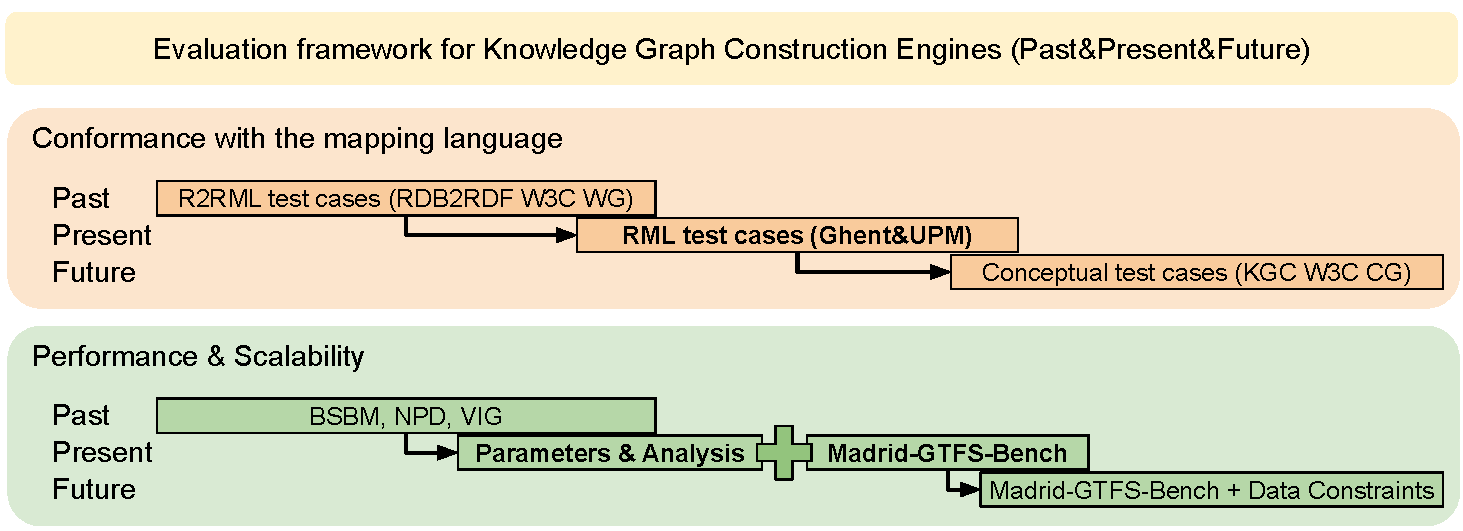
\includegraphics[angle=90,width=0.5\linewidth]{figures/Evaluation Framework.pdf}
    \caption[Evaluation Framework - Past\&Present\&Future]{\textbf{Evaluation Framework - Past\&Present\&Future.} Summarize of the contributions of this chapter and their influence by past contributions and which are going the expected next steps for a include new features in a new version of the evaluation framework.}
    \label{fig:eval-framework}
\end{figure}


\chapter{Exploiting Declarative Annotations for Virtual Knowledge Graph Construction}
\label{chapter:virtual}
%\epigraph{Computer scientists do not make research, they solve real problems}{\textit{Isabel Fraga}}

In this Chapter, we introduce our contributions that exploit declarative annotations over data on the web for enhancing the construction of virtual knowledge graphs. The two frameworks presented apply the \textit{mapping translation} concept defined in Chapter \ref{chapter:mappig-translation} for improving the current proposals. 

Section \ref{chap6_morphgcsv} presents Morph-CSV, a constraint-based approach for ensuring the effectiveness of SPARQL-to-SQL when the input tabular data is not a relational database instance. It uses RML+FnO mapping rules and CSVW metadata descriptions to explicitly declare implicit constraints over the input sources. Section \ref{chap6_morphgraphql} describes Morph-GraphQL, a framework that adapts the SPARQL-to-SQL algorithm presented in~\citep{chebotko2009semantics} to automating the generation of programmer data wrappers from declarative mapping rules. More in detail, it is focused on generating GraphQL resolvers for virtual access to relational databases using R2RML mappings as inputs.

\section{Morph-CSV: Virtual Knowledge Graph Access over Tabular Data}
\label{chap6_morphgcsv}
Guided by the Open Data principles, governments and private organizations are regularly publishing vast amounts of public data in open data portals. For example, almost a million datasets are available in the European Open Data Portal (EODP)\footnote{\url{https://www.europeandataportal.eu}}, and many of them are available in tabular formats (e.g., CSV, Excel), as observed in Table \ref{tab:odp}. Both the simplicity of a tabular representation and the variety of tools to manage a table (e.g., Excel, Calc) have influenced the popularity of tabular formats to represent open data.  

Albeit extensively utilized, tabular representations imposed various data management challenges to advanced users (e.g., developers, data scientists). The lack of a unified way to query tabular data, something available in other formats (e.g., RDB, JSON, XML), hinders the integration of sources, especially those having datatype inconsistencies. Moreover, data may not be normalized, and information about relationships or column names are not always descriptive or homogeneous. Hence, data consumers are usually forced to apply ad-hoc or manual data wrangling processes to consume data via open data portals. 

Following Linked Data~\citep{bizer2011linked} and FAIR initiatives~\citep{wilkinson2016fair}~\footnote{\url{https://www.go-fair.org/fair-principles/}}, data providers are encouraged to make data available in an RDF-based representation following the 5-star linked data principles\footnote{\url{https://5stardata.info/en/}}. The Ontology-Based Data Access (OBDA)~\citep{poggi2008linking} paradigm facilitates the transformation of heterogeneous data into RDF.
An OBDA corresponds to a data integration system (DIS)~\citep{Lenzerini02} over heterogeneous data sources. A DIS unified schema is defined in terms of ontologies, while mapping rules establish a correspondence between the unified schema concepts and the DIS data sources. An OBDA can be materialized or virtual. In a materialized OBDA, the integration of the DIS data sources is physically represented in RDF~\citep{poggi2008linking}. Contrary, in a virtual OBDA, data integration is performed on the fly during query processing; DIS mapping rules are used to translate SPARQL queries into queries against the DIS data sources~\citep{calvanese2017ontop,priyatna2014formalisation}.
Features like functions in mappings~\citep{de2017declarative,junior2016funul} and metadata~\citep{tennison2015model}, (i.e., annotations) are usually used in materialized OBDAs to overcome the aforementioned challenges of tabular data.

Traditional virtual OBDA approaches, usually, rely on loading tabular data into SQL-based systems\footnote{\url{https://github.com/oeg-upm/morph-rdb/wiki/Usage\#csv-files}}$^,$\footnote{\url{https://ontop-vkg.org/tutorial/mapping/primary-keys.html}}(e.g., MySQL, Apache Drill, Spark SQL, Presto) to perform query translation techniques. However, the correctness and optimization of these techniques are supported by the main assumption about the existence of constraints over the source data (i.e., a good physical design of the relational database instance). Their absence during a virtual OBDA process over tabular data directly impacts  completeness and performance of these techniques. Completeness is affected because of heterogeneity issues in data sources (e.g., datatype CSV columns are simply treated as string-type SQL columns). Furthermore, performance is impacted because indexes are not created based on basic relational constraints, i.e., primary and foreign key constraints are not defined in the schema. Consequently, query translation optimization techniques that commonly exploit indexes (e.g., ~\citep{rodriguez2015efficient,priyatna2014formalisation}) may not produce the expected results whenever the constraints have not been applied, or the indexes have not been created.
\begin{table}[t]
\centering
\caption[Formats in EU open data portal]{Most commonly used formats and percentage over the total number of datasets to expose data in mature EU open data portals in October 2019. Each dataset may be shared in different formats.}
\label{tab:odp}
\begin{tabular}{c|c|c|c}
\hline
\rowcolor{orange!20} 
\textbf{Data Portal} & \textbf{1st Format}  & \textbf{2nd Format} & \textbf{3rd Format} \\ \hline
Spain                & \textbf{CSV (50\%)}  & \textbf{XLS (35\%)}  & JSON (33\%)          \\ 
Norway               & \textbf{CSV (77\%)}    & GEOJSON (17\%)         & JSON (14\%)            \\ 
Italy               & \textbf{CSV (76\%)}  & JSON (35\%)          & XML (25\%)           \\ 
Croatia              & \textbf{XLS (63\%)}    & \textbf{CSV (40\%)}   & HTML (33\%)           \\ \hline
\end{tabular}
\end{table}

OBDA annotations such as the W3C recommendation to annotate tabular data, CSVW~\citep{tennison2015model} and some extensions of standard mapping rules (e.g., RML+FnO~\citep{de2017declarative}) are commonly used to describe constraints over an OBDA tabular dataset. For example, we can standardize a column indicating its format, define integrity constraints, or declare data types. The majority of OBDA query translation engines~\citep{priyatna2014formalisation,endris2019ontario} do not include this information. Those engines that have partially included the constraints (e.g., Squerall~\citep{mami2019squerall} parses RML+FnO mapping rules) are not fully documented; i.e., there is no explanation of how these constraints are taken into account. The definition of a workflow that includes the exploitation of these tabular annotations during a virtual OBDA process will ensure correct and optimized SPARQL-to-SQL translations.

\noindent\textbf{Problem Statement:} 
We address the limitations of current OBDA query translation techniques over tabular data, which enforce and demand lots of unreproducible and hard manual work for the application of constraints to ensure efficient query processing and query completeness\footnote{\url{https://github.com/oeg-upm/morph-rdb/wiki/Usage\#csv-files}}$^,$\footnote{\url{https://ontop-vkg.org/tutorial/mapping/primary-keys.html}}$^,$\footnote{\url{https://ontop-vkg.org/tutorial/mapping/foreign-keys.html}}. Our goals are to (i) define a framework that includes the application of a set of constraints over tabular data, and (ii) define a set of efficient operators that apply each type of constraint to improve query completeness and performance (e.g., removal of duplicates, normalization of input sources or application of transformation functions). 

\noindent\textbf{Proposed Solution:} 
We propose a set of new steps to be aligned with the current OBDA workflow. Further, we implement Morph-CSV, and evaluate its behavior embedded on top of two well known open source SPARQL-to-SQL engines, in comparison with previous approaches.

\noindent\textbf{Contributions:} Our main contributions are as follows:
\begin{enumerate}
\item Definition of the concept of Virtual Tabular Dataset (VTD) composed by a tabular dataset and its corresponding OBDA annotations, as well as its alignment with the current definition and assumptions of the OBDA framework~\citep{xiao2018obdasurvey}.
\item Morph-CSV, a framework that implements a constraint-based OBDA workflow for tabular datasets; it receives a VTD and a SPARQL query as inputs and outputs an OBDA instance. Morph-CSV performs the following steps: (i) generation of the constraints based on information on the VTD; (ii) selection of sources and attributes needed to answer the query; (iii) pre-processing of the selected sources applying some of the constraints; and (iv) physical implementation of the corresponding RDB instance and associated schema, ensuring effectiveness of the SPARQL-to-SQL translations and optimizations. Morph-CSV is engine agnostic, i.e., it can be embedded on top of any SPARQL-to-SQL engine.
\item Evaluation of Morph-CSV re-using in the backend two well-known open source SPARQL-to-SQL engines: Morph-RDB~\citep{priyatna2014formalisation} and Ontop~\citep{calvanese2017ontop}; two benchmarks (BSBM~\citep{bizer2009berlin} and GTFS-Madrid-Bench~\citep{chaves2020gtfs}), and a real-world testbed from the Bio2RDF project~\citep{belleau2008bio2rdf} are used in the study.
\end{enumerate}




\subsection{Motivating Example}
\begin{figure}[ht]
    \centering
    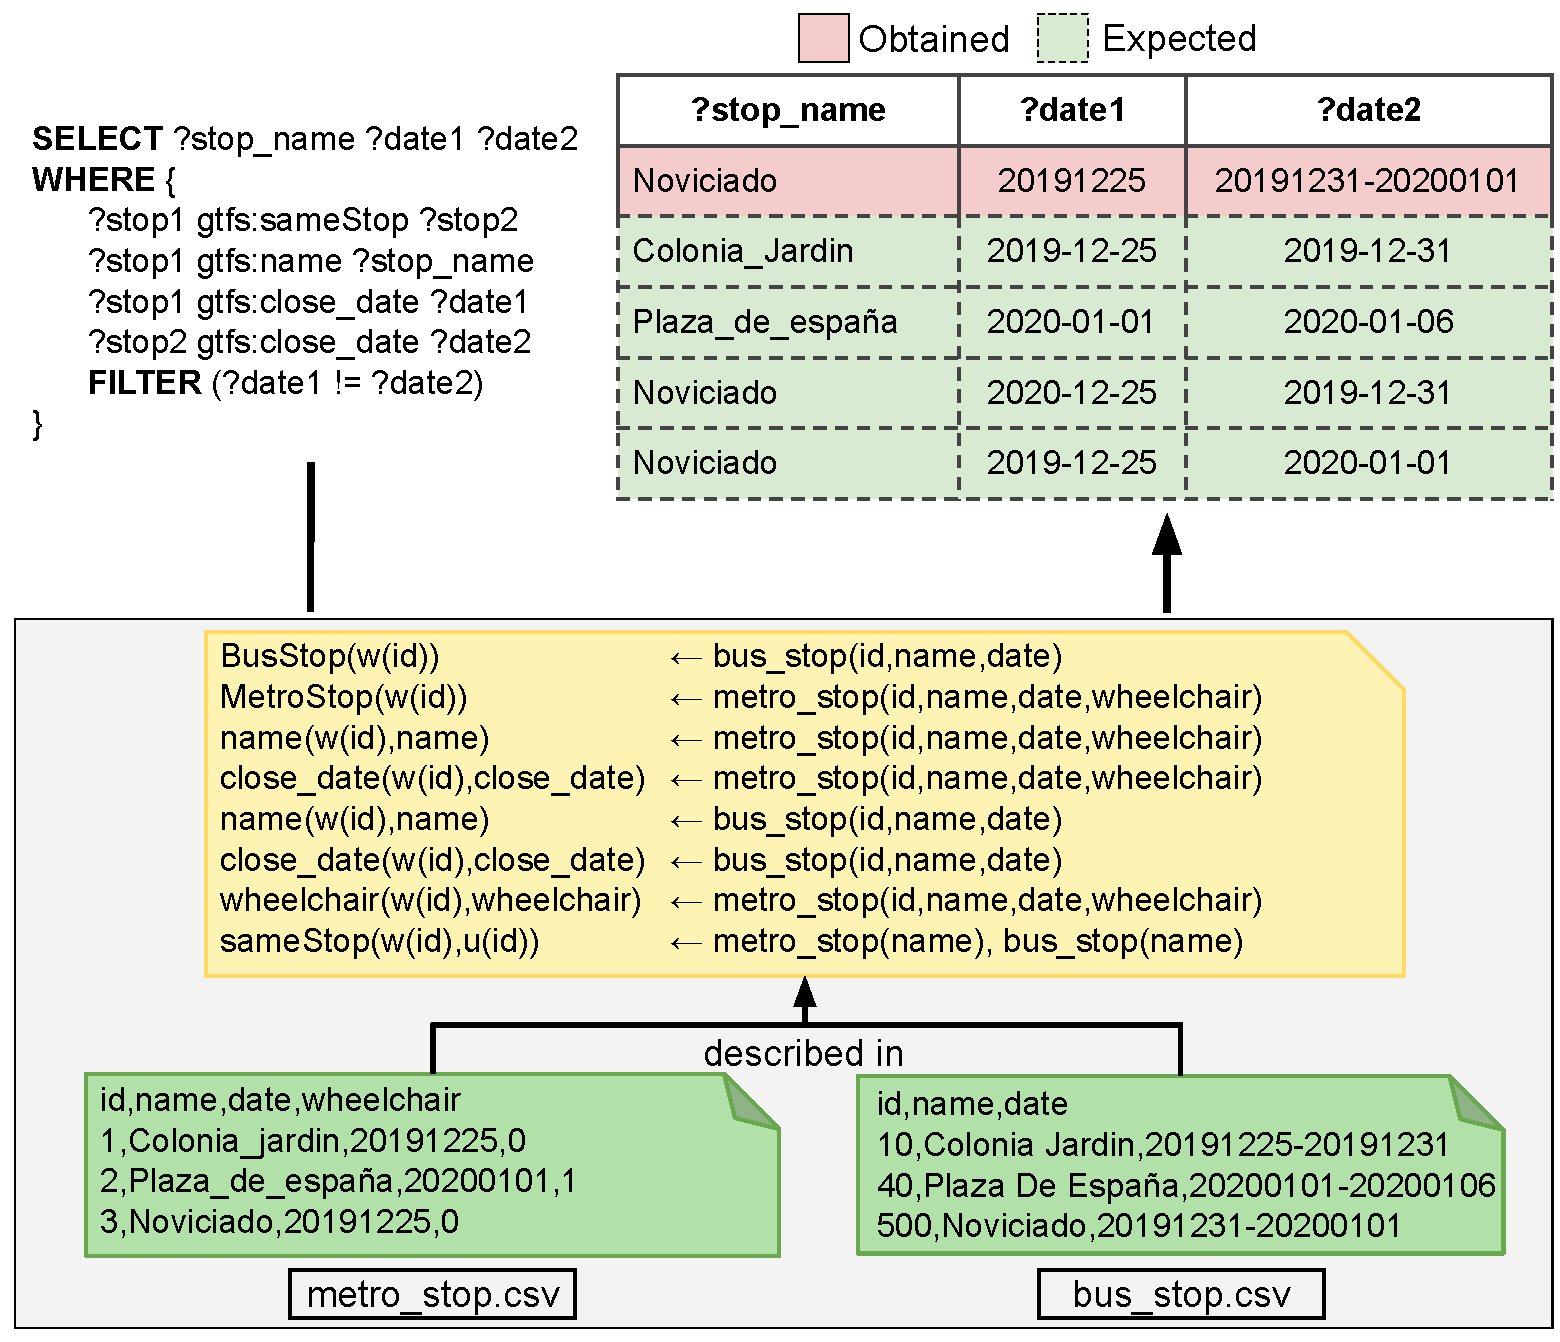
\includegraphics[width=0.6\linewidth]{figures/example.pdf}
    \caption[Morph-CSV motivating example]{\textbf{Motivating Example.} SPARQL query evaluation over two tabular data files in the transport domain through a common OBDA approach. It loads the files as single tables in an SQL-based system and uses the mapping rules for query translation. The number of results differs with respect to the expected results due the heterogeneity of the raw data. Additionally, query performance may be affected by the join condition between the two tables, the absence of indexes and the loading of columns that are not needed to answer the input query (wheelchair).}
    \label{fig:example}
\end{figure}
Since May 2017, the publication of a new directive by the EU Commission on discoverability and access to public transport data across Europe\footnote{\url{https://ec.europa.eu/transport/themes/its/road/action_plan/nap}} has motivated the development of solutions for multi-modal travel information services. This document states that transport data should be available through national access points (NAP), e.g., databases, data warehouses, and repositories. Consider the \emph{de-facto standard} for publishing open data in the transport domain, GTFS\footnote{\url{https://developers.google.com/transit/gtfs/reference/}}. This model enables the representation of transport-related concepts such as \textit{schedules}, \textit{stops,} and \textit{routes}, using 15 different inter-related CSV files called GTFS feed. Following best modeling practices recommended in this model specification, each feed comprises entities of one type of transportation mode (e.g., metro, train, and tram). Linking these feeds based on their stops enables route planners to offer multi-modal routes, a route that can be created using various transportation types.
Albeit straightforward and simple to use, GTFS feeds do not allow for the definition of integrity constraints such as primary or foreign keys. As a consequence, data integrity cannot always be guaranteed. 

Consider the GTFS feeds from the metro and buses of Madrid's city; they have several stops and stations in common. Different transport authorities create them, and the names of their stops are defined in various manners. Although these types of entities can be represented, the unique identification and relationships among them cannot be explicitly expressed. Figure~\ref{fig:example} depicts a portion of these two GTFS feeds. As it is usual in open datasets, stop names do not follow a standard structure (e.g., ``Colonia Jardin'' in \textit{bus\_stops.csv} and ``Colonia\_jardin'' in \textit{metro\_stops.csv}). A similar issue is present in closing dates, where there are multi-valued cells, and their format is not the standard one (e.g., yyyy-MM-dd). Suppose a user is interested in collecting information about bus and metro stops with the same name and information related to their closing dates during holidays; Figure~\ref{fig:example} presents the SPARQL query describing this request. Following the approach commonly employed by typical OBDA engines, the two files would be loaded into an SQL-system and treated as single tables. The obtained result set only contains one answer where the stop names in the two data sources are identical (``Noviciado''). However, the expected result set should include more answers by joining among the bus and metro's stop names through the normalization of multi-valued date columns. 

Query's performance may also be affected whenever a join condition is executed between the stop names of both files. Furthermore, the absence of possible indexes in these joining columns makes ineffective the typical optimizations applied in a SPARQL-to-SQL process. Nonetheless, to effectively exploit the indexes to scale-up the execution of the translated queries, the satisfaction of the unique and foreign integrity constraints should be ensured. The manual and ad-hoc definition of the relational schema representing these tables and the corresponding integrity constraints will overcome this problem. Nevertheless, this task is time-consuming, and reproducibility is not ensured. In this paper, we propose Morph-CSV, a constraint-based OBDA framework capable of exploiting standard tabular data annotations (e.g., RML or CSVW) to generate the required constraints ensure the integrity of the tabular schema in terms of unique identifiers and foreign keys. Moreover, Morph-CSV applies metadata annotation from CSVW to generate domain-specific constraints. As a result, Morph-CSV enhances query completeness and performance of SPARQL-to-SQL techniques, in compliance with OBDA assumptions.


\subsection{Ontology Based Data Access over Tabular Data}
This section describes a set of challenges demanded be addressed whenever tabular data is queried in a virtual OBDA framework. Further, we describe relevant OBDA proposals for annotating tabular datasets and their alignment with the identified challenges.

\subsubsection{Querying challenges under virtual OBDA for tabular data}
There are specific challenges on querying tabular datasets using an OBDA approach that have not been tackled by existing techniques. We will describe those challenges and explain how they may have a negative effect in terms of completeness and performance of query-translation approaches:
\begin{itemize}
    \item \textbf{Updated results:} Existing frameworks load all of the tabular input files that are specified as sources in the OBDA mapping rules into a SQL database before executing the query-translation process. This step has to be repeated whenever a SPARQL query is evaluated to ensure up-to-date results, resulting in unnecessary longer loading time, affecting, thus, OBDA performance.
    \item \textbf{Normalization:} Tabular data formats do not provide restrictions on how to structure data. As a result, cells may contain multiple values, and one file may represent multiple entities. Having non-normalized tables may affect the completeness of the query. When a tabular source with multiple-valued cells is loaded into an RDB table, the cell's value is interpreted by the RDBMS as an atomic value, reducing, thus, completeness for queries that filter or ``join'' on the corresponding column. Representing several entities in a single file may lead to duplicate answers, and in turn, decrease query answering performance.
    \item\textbf{Heterogeneity:} Tabular data normally contain values that need to be transformed before query evaluation (e.g., column default values or normalization of date formats). Since there may be different formats for the same datatype or default values that may have not been included in the dataset, query completeness can be affected.
    \item \textbf{Lightweight Schema:} Most of the tabular data only provide minimal information about their underlying schema in the form of column names in the header, if at all present. Also, although there is implicit information on keys and relationships among sources, there is no way to specify primary key or foreign key constraints. The same can be said on indexes and datatypes. The existence of this type of information is assumed~\citep{xiao2018obdasurvey} in an OBDA approach for performing optimizations in query evaluation techniques. Therefore, the lack of this information affects the performance of OBDA engines.
\end{itemize}

Although some of the aforementioned challenges are not only specific to tabular datasets and are proposed in several data integration approaches~\citep{golshan2017data,halevy2006data,doan2012principles} there are two main reasons why it is important to address these problems in this context: first, the number of tabular datasets available in the web of data is enormous and still growing and these challenges were not taken into account in previous OBDA proposals; second, although there are declarative proposals to handle these issues in the state of the art like CSV on the Web~\citep{tennison2015model} for metadata annotations, or mapping languages that include transformation functions to deal with heterogeneity (e.g., RML+FnO~\citep{de2017declarative} or R2RML-F~\citep{debruyne2016r2rml}), there is not yet a proposal that exploits the information from these inputs including their application in the form of constraints into a common OBDA workflow.



% Please add the following required packages to your document preamble:
% \usepackage{multirow}
% \usepackage{graphicx}
% Please add the following required packages to your document preamble:
% \usepackage{multirow}
% \usepackage{graphicx}
\begin{table*}[t]
\centering
\caption[Relevant properties of CSVW and RML+FnO]{Properties of CSVW and RML+FnO that can be used to address the challenges of dealing with tabular data in a virtual OBDA approach}
\label{tab:features}
\resizebox{0.9\textwidth}{!}{%
\begin{tabular}{c|l|l}
\hline
\rowcolor{orange!50} 
\textbf{General Challenge} & \multicolumn{1}{c|}{\textbf{Detailed Challenges}} & \multicolumn{1}{c}{\textbf{Relevant Properties}} \\ \hline
 Updated results & Select relevant sources and columns &  SPARQL + RML+FnO\\ \hline
\multirow{4}{*}{\begin{tabular}[c]{@{}c@{}}Lightweight\\ Schema\end{tabular}} & Describe the corresponding concept & rr:class \\ \cline{2-3} 
 & Describe the corresponding property & rr:predicateMap \\ \cline{2-3} 
 & Specify NOT NULL constraint & csvw:required \\ \cline{2-3} 
 & Column datatype & csvw:datatype \\ \hline
\multirow{7}{*}{Heterogeneity} & Domain values & csvw:minimum, csvw:maximum \\ \cline{2-3} 
 & Specify the format of a column & csvw:format \\ \cline{2-3} 
 & Transform value & fnml:functionValue \\ \cline{2-3} 
 & Default for missing values & csvw:default \\ \cline{2-3} 
 & Specify NULL values & csvw:null \\ \cline{2-3} 
 & Add header to a CSV file & csvw:rowTitles \\ \hline
\multirow{4}{*}{Normalization} & Primary Key & csvw:primaryKey \\ \cline{2-3} 
 & Foreign Key & csvw:foreignKey \\ \cline{2-3} 
 & Relationships between columns & rr:parentTriplesMap + rr:joinCondition \\ \cline{2-3} 
 & Mutiple entities in one source & rr:TriplesMap + rml:logicalSource \\ \cline{2-3} 
 & Support for multiple values in one cell & csvw:separator \\ \cline{2-3} 
 \hline
\end{tabular}%
}
\end{table*}

\subsubsection{OBDA annotations for tabular data}
R2RML~\citep{R2RML} is a W3C Recommendation for describing transformation rules from RDB to RDF and a widely used mapping language in virtual OBDA approaches. RML~\citep{dimou2014rml} extends R2RML; it provides support to a variety of data formats, e.g., XML, CSV, and JSON. Both languages provide basic transformation functions to concatenate strings, which are especially useful for generating URIs from columns/fields of the dataset. Recently, RML has been integrated with the Function Ontology (FnO)~\citep{de2016ontology} to support other types of transformations. Additionally, for tabular data, CSVW metadata~\citep{tennison2015model} is a W3C Recommendation to describe tabular datasets. Although there are other proposals in the state of the art to deal with some of the aforementioned challenges~\citep{junior2016funul,debruyne2016r2rml}, Morph-CSV relies on these two proposals because they cover the identified challenges. Additionally, this election is supported by the fact that CSVW is a recommendation from the W3C and RML+FnO (besides being a extended version of a W3C recommendation) has been previously applied in other projects~\citep{de2017declarative,mami2019squerall} and is widely used by several materialization engines, e.g.,  RMLMapper\footnote{https://github.com/RMLio/rmlmapper-java}, CARML\footnote{https://github.com/carml/carml/} and RocketRML~\citep{csimcsek2019rocketrml}. Finally, relevant benefits of these annotations are that both of them are defined in a declarative manner. Thus, the maintainability, the readability, and the understanding of the virtual OBDA approach is improved and independent from any specific programming language.

In Table \ref{tab:features}, we summarize the relevant properties from RML+FnO and CSVW that can be used to address the  challenges identified in the previous section. Additionally, we provide a detailed description of these properties:
\begin{itemize}
    \item \textbf{Metadata.} The property \texttt{csvw:rowTitles} can be used to specify column names in case the first row is not used to specify them.
    
    \item \textbf{Transformation functions.} String concatenation functions are supported by both CSVW (\texttt{csvw:aboutUrl}, \texttt{csvw:valueUrl}) and the RML property (\texttt{rr:template}). In addition, more complex functions can be declaratively specified using RML+FnO, specifically, with the \texttt{fnml:functionValue} property. Finally, two special cases of transformation functions in the context of OBDA are related to how default values and NULL representations have to be generated in the RDB instance. These two cases can be handled by CSVW properties: \texttt{csvw:defaultValue} and \texttt{cvwv:null}.
    
    \item \textbf{Domain Constraints.} CSVW allows for the specification of the datatype (\texttt{csvw:datatype} property) and format (\texttt{csvw:format} property) of tabular columns. CSVW also provides a couple of properties (e.g., \texttt{csvw:mininum} or \texttt{csvw:maximum}) to specify the range of numerical columns and a property \texttt{csvw:required} to specify the NOT NULL constraint over the column of a table.
    
    \item \textbf{Integrity Constraints.} In CSVW the property \texttt{csvw:primaryKey} can be used to declare explicitly the primary key of a table. As for the foreign key, the use of RML's properties \texttt{rr:parentTriplesMap} together with the property \texttt{rr:joinCondition} can be seen as an indication that the parent column used over this rule could be a foreign key, or at least that a relation exists. CSVW provides an explicit way to declare whether a column is a foreign key, using the \texttt{csvw:foreignKeys} property. 
    
    \item \textbf{Normalization.} The property \texttt{csvw:separator} from CSVW indicates the character used to separate multiple values in the cells of a CSV column, which is relevant when a CSV file is in 1NF. Multiple RML TriplesMap using the same data source can be used as an indication that the source contains multiple concepts (2NF).
\end{itemize}



\subsection{The Morph-CSV Framework}

The formal framework presented in~\citep{xiao2018obdasurvey} defines an OBDA specification as a tuple $P$ = $\langle O,S,M\rangle$ where $O$ is an ontology, $S$ is the source schema, and $M$ a set of mappings. Additionally, an OBDA instance is defined as a tuple $PI$ = $\langle P,D\rangle$ where P is an OBDA specification and $D$ is a data instance conforming to $S$. In a virtual OBDA framework, queries are posed over a conceptual layer and then translated to queries over the data layer using information in the mappings. There is a set of assumptions over the framework that support the possibility of doing query translation and  ensuring  semantic preservation in the process, together with the application of  optimization techniques proposed in the state of the art. To motivate our proposal, we have to establish what are the main assumptions made in previous proposals and their impact when data is represented in tabular form.


\begin{figure}[ht]
  \centering
  \subfloat[Baseline approach]{
    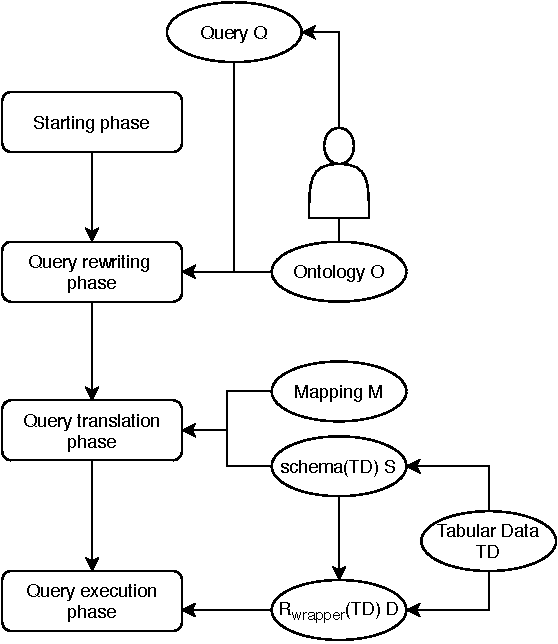
\includegraphics[width=0.48\linewidth]{figures/naive-approach.pdf}  
    \label{fig:naive}
  }
  \subfloat[Enhanced virtual OBDA workflow.]{
  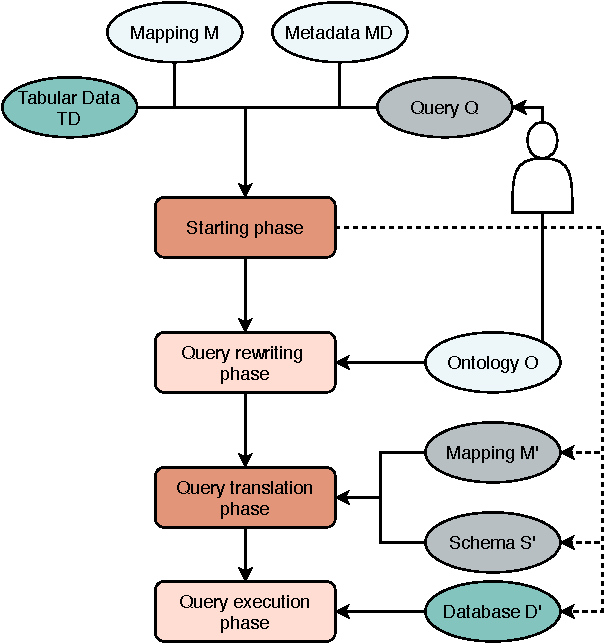
\includegraphics[width=0.48\linewidth]{figures/vtd-approach.pdf} 
  \label{fig:vtd}
  }
\caption[Virtual OBDA for tabular data approaches]{\textbf{Virtual OBDA for tabular data approaches.} The baseline approach creates the schema and relational database instance extracting file and columns names from the tabular dataset. The proposed workflow exploits the information from the mapping rules and metadata to extracted a set of constraints and applying them over the tabular data to generate the schema and the relational database instance.}
\label{fig:obda}
\end{figure}


\subsubsection{OBDA assumptions}
Analyzing the definition of OBDA in~\citep{xiao2018obdasurvey} and its extension for NoSQL databases defined in~\citep{botoeva2019ontology} we identified a set of assumptions made over the framework and their impact when the dataset is tabular:
\begin{itemize}
    \item There is a native query language $QL$ for $D$. For a tabular dataset, there is no native query language for querying this format, which generates an important difference with other common formats for exposing raw data on the web such as JSON and XML as they include methods to query them (JSONPath, XPath). This is the main issue that needs to be solved in order to query tabular datasets in a virtual OBDA context and has a direct impact on the rest of the assumptions.%, that have been solved in a naive manner.
    \item $S$ typically includes a set of domain and integrity constraints. In the case of querying a tabular dataset $D_{tabular}$, $S$ is defined using column names extracted from $D_{tabular}$ and it does not include any  constraint types (neither domain nor integrity constraints). This has a negative impact not only in terms of query execution time but also over query result completeness as there will be queries that cannot be executed due to the lack of explicit domain constraints.
    \item $D$ is an RDB instance or  a NoSQL database instance, %equipped with 
    that includes an RDB wrapper able to provide a relational view over $S$ and $D$. In the context of a tabular dataset $D_{tabular}$, $D$=$R_{wrapper}(D_{tabular})$ where $R_{wrapper}$ is a relational database wrapper that satisfies $S$.
    %contains raw data that needs to be loaded according to (the generated) $S_{naive}$ in order to be queried, so a function $load(S_{naive},D_{tabular})$ creates an RDB instance $D$, loading the raw data in $D_{tabular}$. This has an impact over the total query execution time as the system has to load all the data into the RDB instance before running the query translation and execution process.
\end{itemize}

\begin{figure}[!ht]
    \centering
    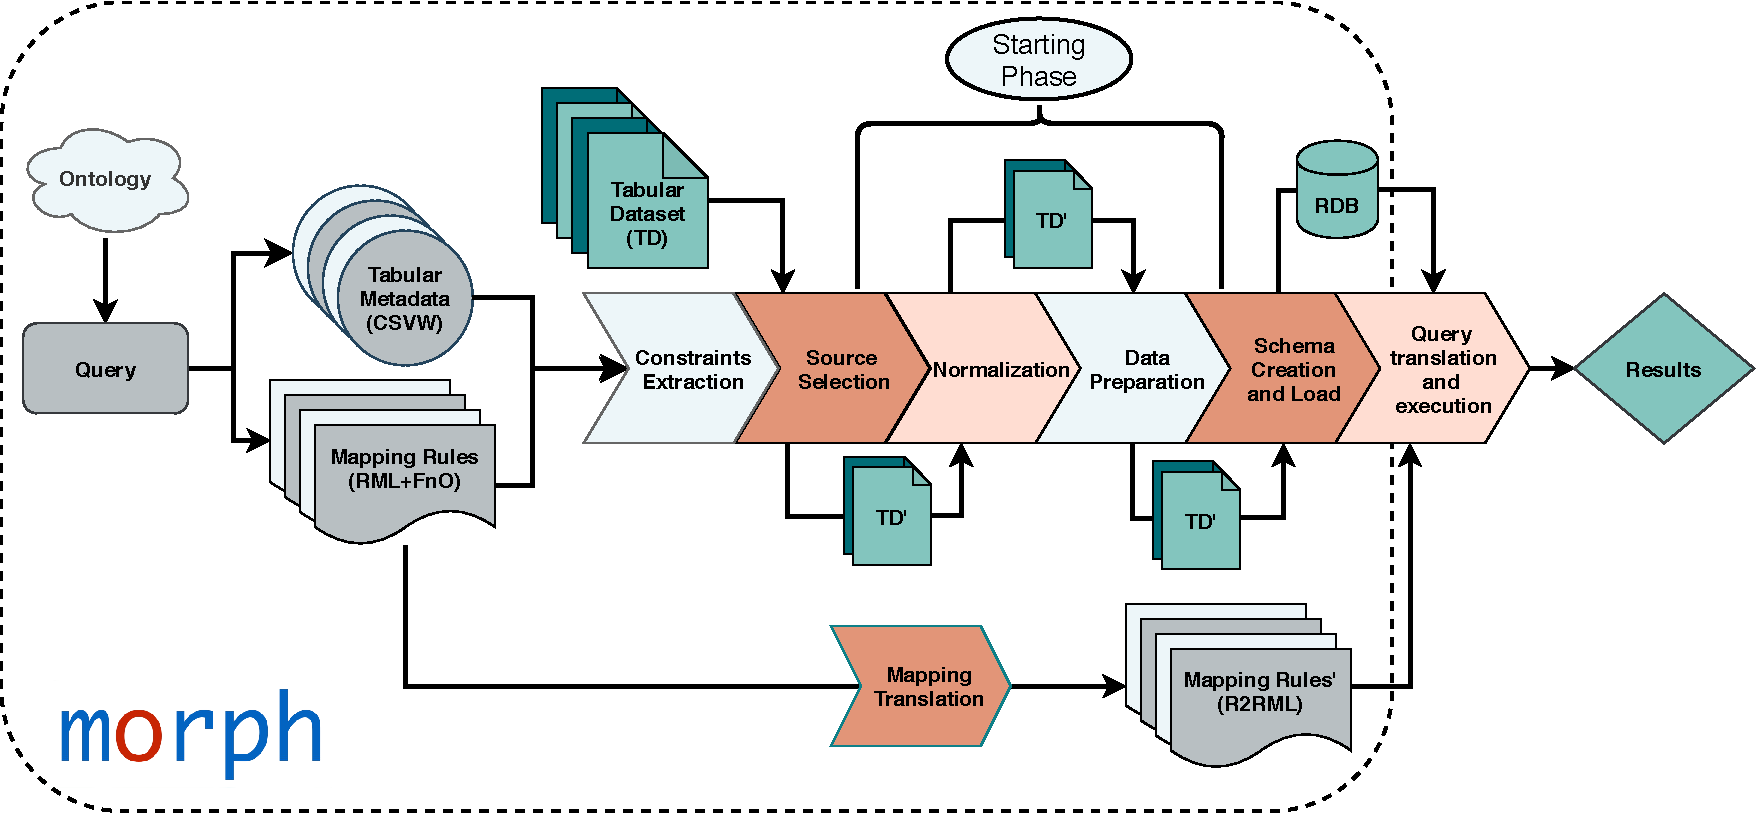
\includegraphics[width=1\linewidth]{figures/architecture.pdf}
    \caption[The Morph-CSV Framework.]{\textbf{The Morph-CSV Framework.} Morph-CSV extends the starting phase of a typical OBDA system including a set of steps for dealing with the identified tabular data querying challenges. The framework first, extracts the constraints from mappings and tabular metadata and then, implements them in a set of operators that are run before executing the query translation and query execution phases, which can be delegated to any SPARQL-to-SQL engine. The mapping rules are translated accordingly to the modified tabular dataset to allow its access by the underlying OBDA engine.}
    \label{fig:workflow}
\end{figure}
\subsubsection{From a virtual tabular dataset to an OBDA instance}
Based on the previous OBDA assumptions, we define the concepts and functions to address the problem of querying a tabular dataset in OBDA.
\begin{definition}
\label{def:vtd}
A virtual tabular dataset is defined as a tuple $VTD$=$\langle D_{tabular},O,M,MD\rangle$ where $D_{tabular}$ is a tabular dataset that is composed of a set of data sources, defined as $\mathcal{D}_{tabular}$ = $\{s_1,\ldots, s_n\}$ and where each $s_i$ is a tabular relation defined over the domains of the attributes $Att(s_i)=\{A_{i1},\ldots,A_{im}\}$\footnote{A relation is defined as the subset of the Cartesian product of the domains of the attributes.}, where $m$ is the number of attributes of $s_i$. $O$ is an ontology, and $M$ is a set of global as view mappings between $O$ and $schema(D_{tabular})$\footnote{The set of the attributes of each tabular relation in $D_{tabular}$, i.e., $schema(D_{tabular})=\{Att(s_i),\ldots,Att(s_n)\}$}. $MD$ is a set of metadata tabular (domain) annotations, where for each $s_i$ there exists a set $\{(A_{i1},Type(A_{i1})),\ldots,(A_{im},Type(A_{im}))\}$ in $MD$. 
\end{definition}

\textit{Example 1.} The virtual tabular dataset of the GTFS of Madrid's metro system can be defined as $VGTFS^{metro}_{madrid}$ where the dataset is composed by of 10 different tabular sources in CSV format $GTFS_{tabular}$, $LinkedGTFS$\footnote{\url{https://lov.linkeddata.es/dataset/lov/vocabs/gtfs}} is the ontology, the mappings $RML+FnO_{GTFS}$, following the RML+FnO~\citep{de2017declarative} specification, define the relation between the input sources and the ontology and, finally, the metadata $CSVW_{GTFS}$ is defined according to the W3C recommendation, CSVW~\citep{tennison2015model}, specifying a set of constraints extracted from the GTFS reference data model\footnote{\url{https://developers.google.com/transit/gtfs/reference}}.


Given a $VTD$, we define the function $\theta(VTD)=PI$ where $PI$ is an OBDA instance $PI=\langle P,D\rangle$ where $D$=$R_{wrapper}(D_{tabular})$ and $P=\langle O,S,M\rangle$ is an OBDA definition where $S$ does not contain any type of constraint.
We extend the function $\theta(VTD)$ with the aim of enhancing the virtual OBDA baseline approach over tabular data. We define $\theta^{++}(VTD)$=$PI$ as a function that extracts a set of constraints from $M$ and $MD$ and then applies them over $D_{tabular}$ to obtain $PI$. More in detail, the function can be expressed as $\theta^{++}(VTD)$=$\gamma(D_{tabular},O,M,\psi(M,MD))$ where the function $\psi(M,MD)= C$ extracts a set of constraints from OBDA annotations for tabular data. Then, $\gamma(D_{tabular},O,M,C)$ applies the constraints $C$ over $D_{tabular}$ to create a relational database schema $S^{'}$ and its corresponding instance $D^{'}$. In summary, the final output is an OBDA instance $PI^{'}=\langle P^{'},D^{'}\rangle$, where $D^{'}$ is a relational database instance that is compliant with the main assumptions of the OBDA framework and $P^{'}=\langle O,S^{'},M^{'}\rangle$ where $S^{'}$ contains a set of domain and integrity constraints and $M^{'}$ are the mapping rules that define the relations between $O$ and $S^{'}$. Following the proposed workflow in Figure \ref{fig:vtd}, the user first defines the query based on the concepts defined in the ontology, and then, during the starting phase, the $\theta^{++}(VTD)$ is performed. During the execution of the function, first, the constraints from mappings and annotations ($\psi(M,MD)$) are extracted, and then the OBDA instance $PI^{'}$ is generated where the constraints are applied to efficiently create the schema $S^{'}$ and the relational database instance $D^{'}$. Mapping rules are also translated, from $M$ to $M{'}$ to be aligned with the new created schema.
\begin{table}[t]
\centering
\caption[Functions and annotations applied by Morph-CSV]{Summary of constraints, corresponding functions and OBDA annotations applied by Morph-CSV}
\label{tab:summary}
\resizebox{0.9\textwidth}{!}{%
\begin{tabular}{l|l|l|l|l}
\hline
\rowcolor{orange!50}
\multicolumn{1}{c|}{\textbf{Step}} & \multicolumn{1}{c|}{\textbf{Constraint/Improvement}} & \multicolumn{1}{c|}{\textbf{Rule/Annotation}} & \multicolumn{1}{c|}{\textbf{Function}} & \multicolumn{1}{c}{\textbf{Challenge}} \\ \hline
\multirow{2}{*}{Extraction} & \multirow{2}{*}{Reduce search space} & SSG from Query & select\_annotations & \multirow{2}{*}{Selection} \\ \cline{3-4}
 &  & Mapping Rules & select\_sources &  \\ \hline
\multirow{2}{*}{\begin{tabular}[c]{@{}l@{}}Data \\ Normalization\end{tabular}} & 2NF & csvw:separator & split & \multicolumn{1}{c}{\multirow{2}{*}{Normalization}} \\ \cline{2-4}
 & 3NF & \begin{tabular}[c]{@{}l@{}}TriplesMap with\\ same source\end{tabular} & cut & \multicolumn{1}{c}{} \\ \hline
\multirow{3}{*}{\begin{tabular}[c]{@{}l@{}}Data \\ Preparation\end{tabular}} & \multirow{2}{*}{Standarization} & \begin{tabular}[c]{@{}l@{}}csvw:null, csvw:default\\ csvw:format, etc.\end{tabular} & sub & \multicolumn{1}{c}{\multirow{3}{*}{Heterogeneity}} \\ \cline{3-4}
 &  & fnml:functionValue & create & \multicolumn{1}{c}{} \\ \cline{2-4}
 & Duplicates & - & duplicates & \multicolumn{1}{c}{} \\ \hline
\multirow{4}{*}{\begin{tabular}[c]{@{}l@{}}Schema \\ Creation and\\ Load\end{tabular}} & Primary Key & csvw:primaryKey & primaryKey & \multirow{4}{*}{\begin{tabular}[c]{@{}l@{}}Lightweight \\ Schema\end{tabular}} \\ \cline{2-4}
 & Foreign Key & csvw:foreignKey & foreignKey &  \\ \cline{2-4}
 & DataType & csvw:datatype & datatype &  \\ \cline{2-4}
 & Index & \begin{tabular}[c]{@{}l@{}}selectivity on mapping \\ join conditions\end{tabular} & index &  \\ \hline
\end{tabular}%
}
\end{table}
\textit{Example 2.} The process of applying the function $\theta^{++}(VGTFS^{metro}_{madrid})$ generates the OBDA instance $PIGTFS^{metro}_{madrid}$. The features of this output are a relational database schema $GTFS_{schema}$, a relational database instance $GTFS_{SQL}$ compliant with the defined schema, and a set of mapping rules following the R2RML W3C recommendation, $R2RML_{GTFS}$, that represent the relations between $GTFS_{schema}$ and the $LinkedGTFS$ ontology. 


Constraints are conjunctive rules specified for tabular data that restrict the valid data in one or more tables. $C$ is a set of constraints, where each constraint $c$ is a logical statement that expresses the condition that needs to be satisfied by the data in order to be valid. Each constraint is applied through a function.

\textit{Example 3.} CSVW allows expressing a primary key constraint for a table. The function $\psi(M,MD)=C$ generates the corresponding constraints in the form of a function $primaryKey(t,a)$ that applies this constraint to a source $t$ and a set of columns $a$, and generates a primary key in the output schema. 

Given an OBDA instance $PI$=$\langle\mathcal{P,D}\rangle$, we define the function $eval(Q,PI)$, that retrieves a SPARQL answer set that is the result of the translation of $Q$ from SPARQL to SQL using the mapping rules $M$ defined in $P$, and then evaluating the query directly over $D$. 


\subsubsection{Problem statement and solution}
Based on the preliminaries and assumptions on the OBDA framework, we now define the problem that we address in this paper and Morph-CSV, our proposed solution.

\paragraph{}\noindent\textbf{Problem statement:} Given a $VTD$, the problem of OBDA query translation over tabular data is defined as the problem of explicitly enforcing implicit constraints $C$ extracted from mapping rules $M$ and metadata $MD$ on a tabular dataset $D_{tabular}$, such that: 
\begin{itemize}
    \item The number of results obtained in the evaluation of the SPARQL query $Q$ over the function $eval(Q,\theta^{++}(VTD))$ is equal or greater than the number of results in the evaluation of the same query $Q$ over the function $eval(Q,\theta(VTD))$, i.e., $\#answers(eval(Q,\theta^{++}(VTD))) \geq \\ \#answers(eval(Q,\theta(VTD)))$.
    \item The total execution time of evaluating a SPARQL query $Q$ over $eval(Q,\theta^{++}(VTD))$ is %decreased compared to the evaluation of the 
    less than or equal than the total execution time of the same SPARQL query $Q$ over the function $eval(Q,\theta(VTD))$, i.e.,\\ $time(eval(Q,\theta^{++}(VTD))) \leq \\
    time(eval(Q,\theta(VTD)))$. 
\end{itemize}


\noindent\textbf{Proposed solution:} We propose Morph-CSV, an alternative to the traditional OBDA workflow for query translation when the input is a tabular dataset (see Figure \ref{fig:vtd}). Morph-CSV relies on the function $eval(Q,\theta^{++}(VTD,\psi(M,MD)))$, to apply the tabular dataset constrains. Thus, Morph-CSV extends a typical OBDA workflow by including a set of steps for a maintainable extraction and efficient application of constraints. The workflow proposal is as follows:
\begin{itemize}
    \item \textbf{Constraint Extraction}: the evaluation of the function $\psi(M,MD)$ produces as output the set of constraints $C$; it exploits the information defined in the annotations of $M$ and $MD$, i.e., the set of metadata tabular annotations and mapping rules, respectively. At implementation level they are expressed as CSVW specifications and RML+FnO mapping rules. 
    \item \textbf{Source Selection}: in this step the sources required to evaluate the SPARQL query $Q$ are selected. The required data sources correspond to the set of sources in the result of unfolding~\citep{poggi2008linking} $Q$ according to the mapping rules in $M$. 
    \item \textbf{Normalization}: metadata and mapping rules are used to extract functional dependencies between the attributes of the data sources. The algorithm by Beeri et al. \citep{Beeri1978ASI} is followed to transform tabular data sources into tabular relations that meet third normal form (3NF).  
    \item \textbf{Data Preparation}: application of the transformation functions based on the extracted domain constraints and on a set of optimization techniques that adapt the ideas proposed in~\citep{jozashoori2019mapsdi,iglesias2020sdm,jozashoori2020funmap} to a virtual OBDA environment. 
    \item \textbf{Schema Creation and Load}: creation of the schema and loading the data into the database instance applying a set of rules for index creation. 
    \item \textbf{Query Translation and Execution}:the evaluation of the query $Q$ is delegated to any OBDA SPARQL-to-SQL engine.
\end{itemize}
 We show the workflow of Morph-CSV in Figure \ref{fig:workflow} with the inputs and outputs of each step. 


\begin{figure}[ht]
  \centering
  \subfloat[Input SPARQL query.]{
  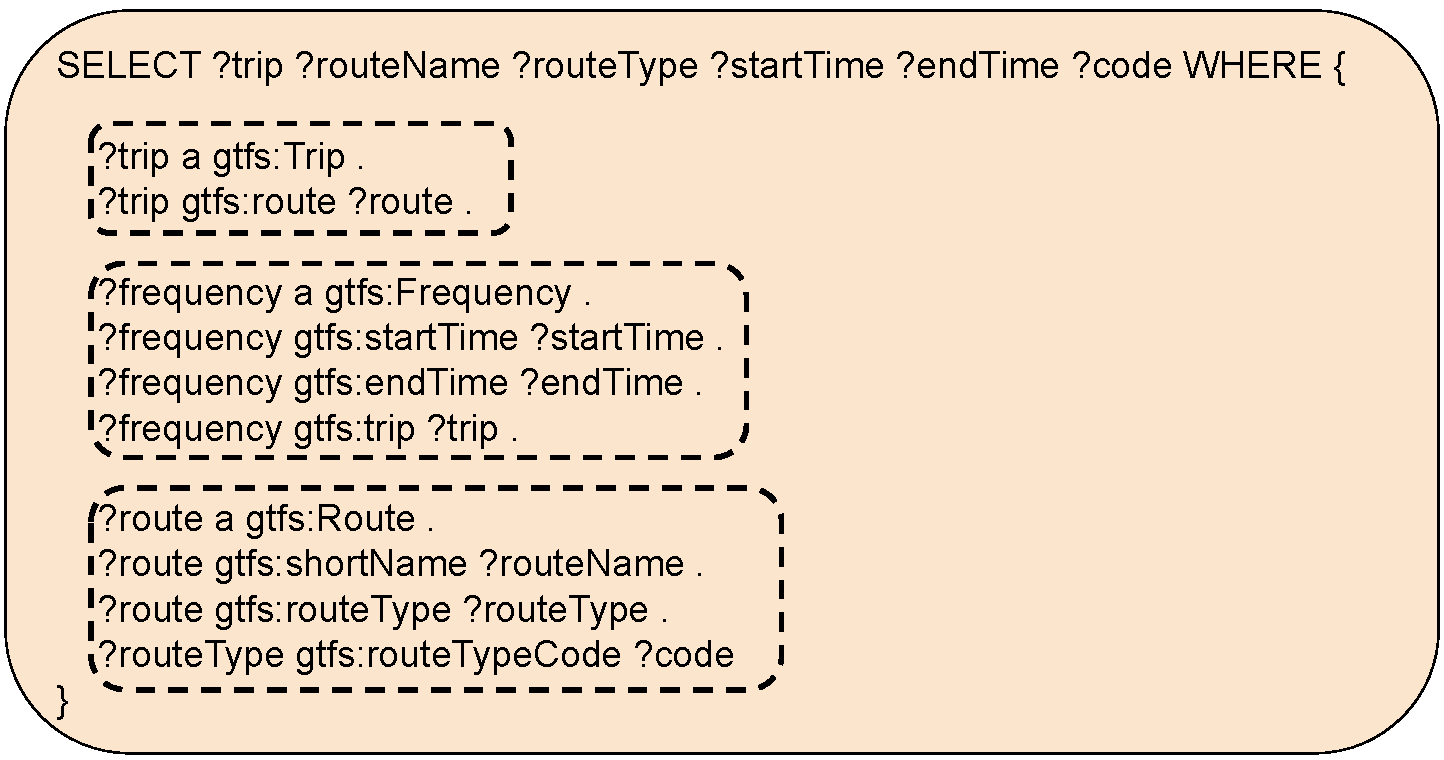
\includegraphics[width=0.5\linewidth]{figures/steps/selectquery.pdf}
  \label{fig:selectionq}
  } 
  \subfloat[Mapping rules selection.]{
    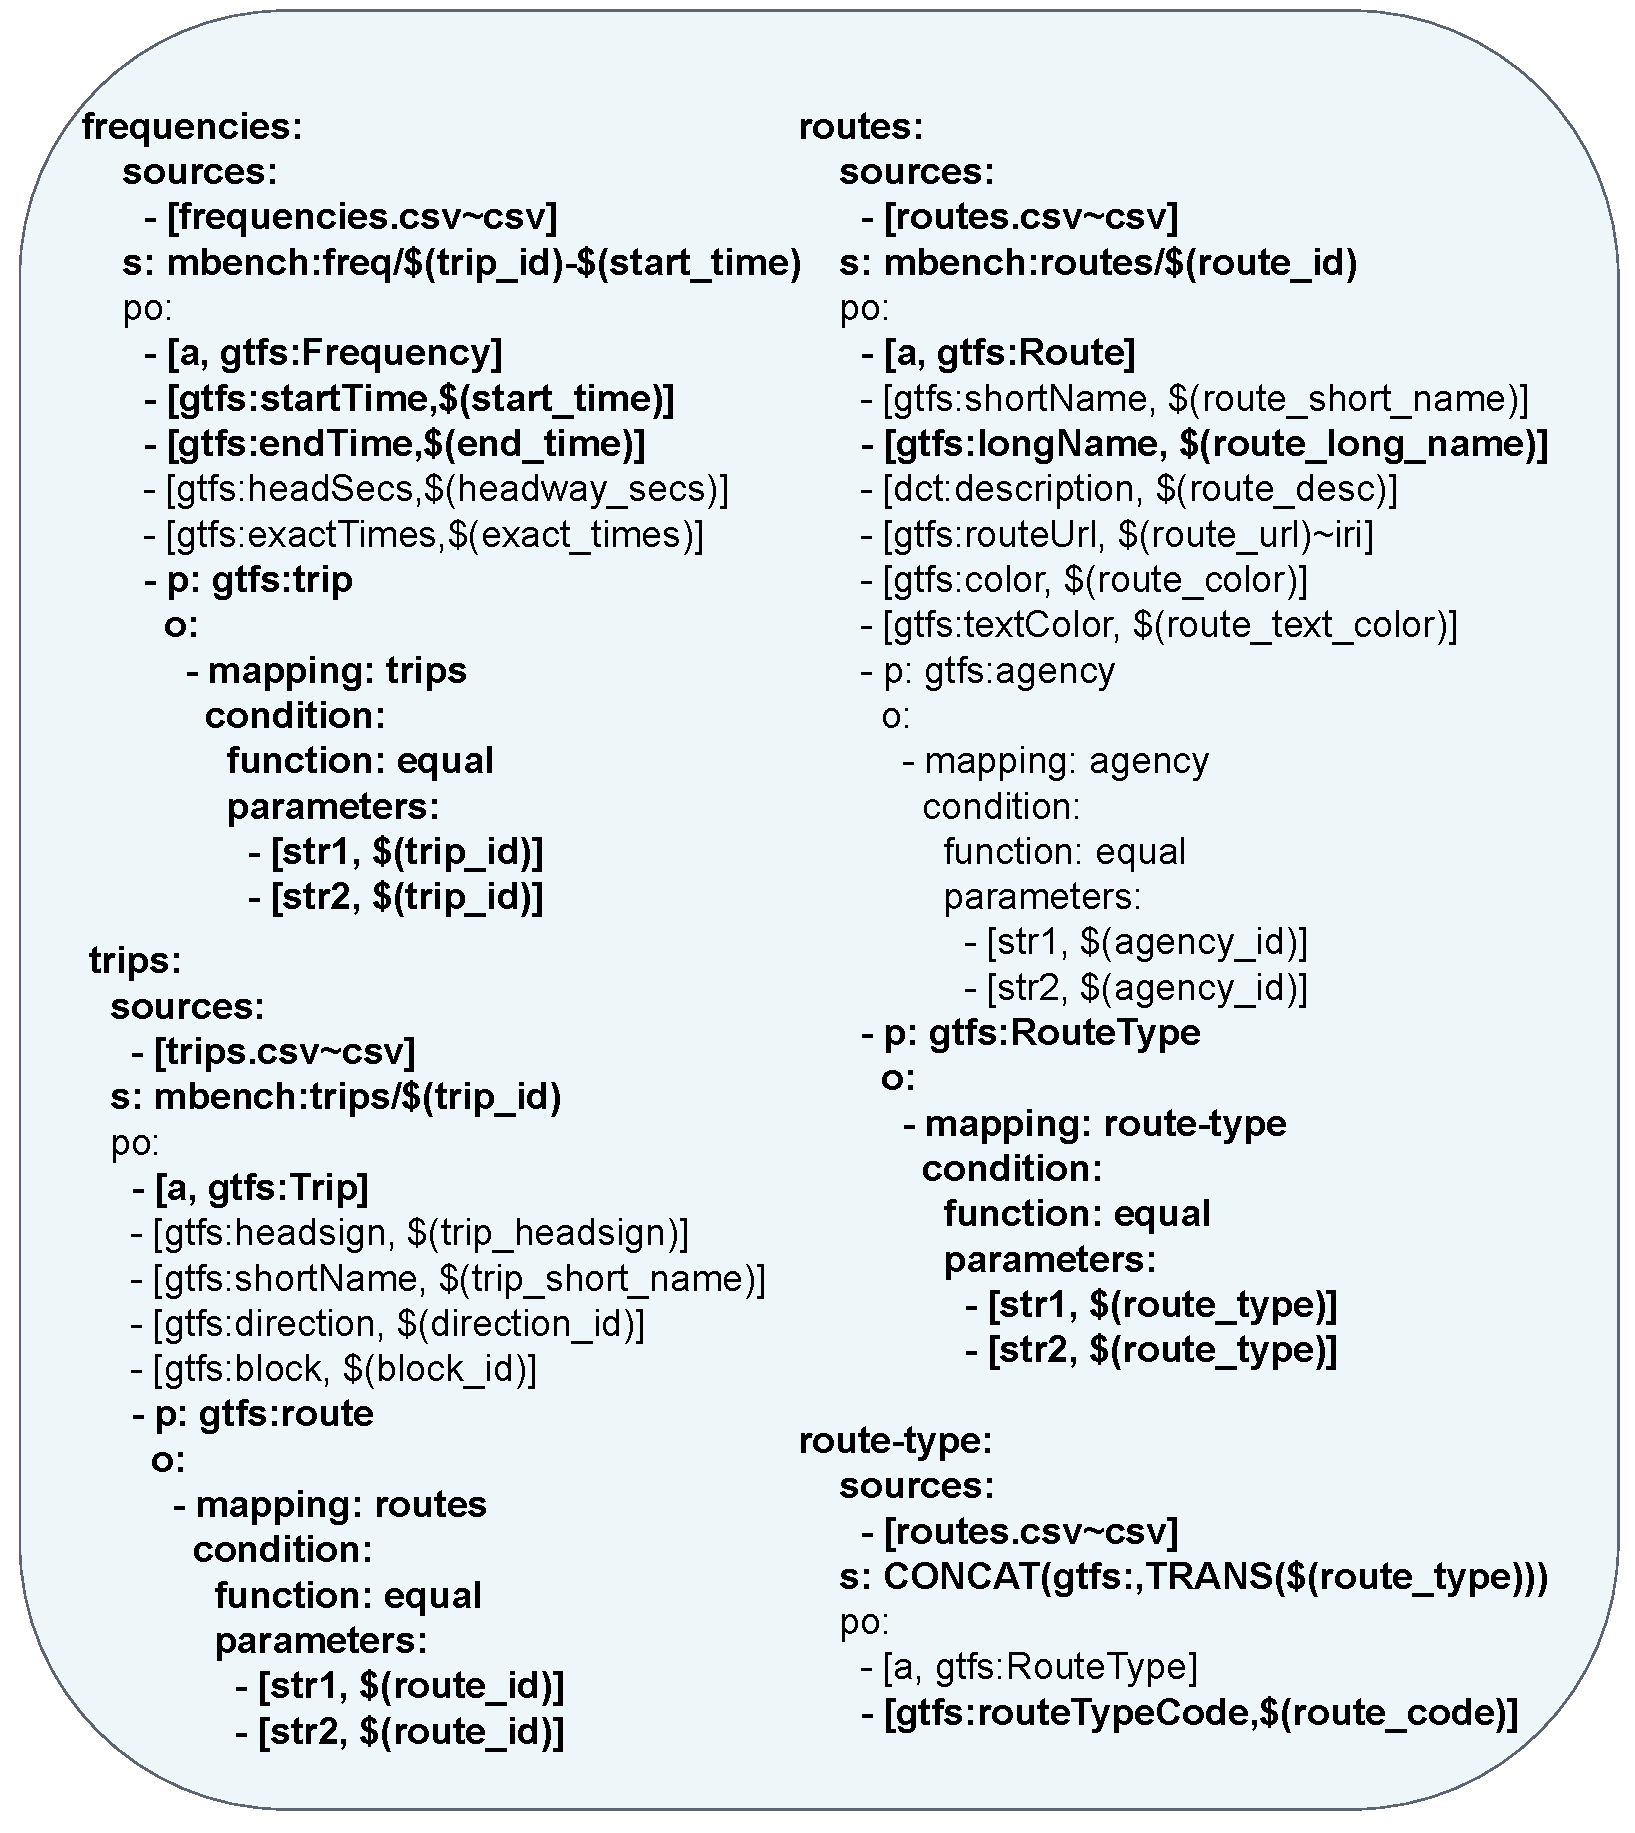
\includegraphics[width=0.5\linewidth]{figures/steps/selectmapping.pdf}  
    \label{fig:selectionm}
  }
\caption[Selection of mapping rules]{\textbf{Selection of Mapping Rules.} Based on the SPARQL query relevant rules are selected (in bold), the rest are discarded.}
\label{fig:selection}
\end{figure}

\subsubsection{Steps performed in the Morph-CSV framework}
We describe in detail the steps proposed in Morph-CSV together with an example extracted from the benchmark for virtual knowledge graph access, Madrid-GTFS-Bench, using the query shown in Figure \ref{fig:selectionq}, the GTFS feed from the  Madrid metro as source data, and the corresponding RML+FnO mapping rules and CSVW annotations\footnote{Resources at: \url{https://github.com/oeg-upm/gtfs-bench}}.

\subsubsection*{Constraint Extraction}
The first step performed by Morph-CSV is the extraction of the constraints that are applied to improve query execution and completeness. Morph-CSV benefits from having declarative and standard approaches to generalize this step: CSVW~\citep{tennison2015model} for the metadata; and RML+FnO~\citep{de2017declarative} for mapping rules and specific transformation functions. Thus, maintainability, understandability and readability of this process are improved in comparison with ad-hoc pre-processing approaches. 

Most of the constraints such as PK-FK relations, datatypes or NULL values are explicitly declared in the metadata of the sources. However, there are a set of implicit constraints such as the conditions for the normalization of sources and the creation of indexes, that require complex rules to extract them and that are explained in detail in the corresponding steps. The summary of the constraints, associated functions, and properties used from OBDA annotations to extract them, are shown in Table~\ref{tab:summary}.


\subsubsection*{Source selection}
The second step is to select the relevant sources to answer the input query. The baseline approach delegates this step to the RDBMS: it loads all the sources of the dataset in the RDB instance because it does not have information about which sources are going to be queried. This has a negative impact in the total execution time of a query. Taking the input mapping rules, Morph-CSV performs query unfolding, and pushes down source selection by executing the function $select(Q,M)$, divided into two main steps. First, Morph-CSV performs an operation to select only the relevant annotations for answering the input query, $select\_annotations(Q,M)$. It first creates the set of star shaped groups SSG$_1\ldots $SSG$_n$ of the query~\citep{vidal2010efficient} (triple patterns with the same subject)\footnote{As usual in these approaches, we assume bounded predicates in the triple patterns}. Then, for each SSG$_i$ and \texttt{rr:TriplesMap} $TM_j$ defined in $M$, the engine selects the $TM_j$ where the predicates in SSG$_i$ are contained in the set of \texttt{rr:PredicateObjectMap} (POMs) defined in $TM_j$. Finally, for each selected \texttt{rr:TriplesMap} $TM_j$, Morph-CSV only selects the POMs according to the predicates defined in the SSG$_i$, hence, removing from each $TM_j$ irrelevant rules for the input query. Using these mapping rules $M^{'}$, only relevant metadata annotations are also selected, $MD^{'}$. The obtained mapping rules in this step, $M^{'}$ and annotations $MD^{'}$, substitute the original ones in $VTD$. An example of this step is shown in Figure \ref{fig:selection}, where the input query asks for trips, their route type, routes names and corresponding time frequencies. Morph-CSV first creates the SSGs, 3 in this case, and using the predicates of each SSG, the \texttt{rr:TriplesMap} are selected from the general GTFS mapping document, discarding the rest of the rules. Then, it only selects the necessary POMs for evaluating the query such as \texttt{gtfs:startTime}, \texttt{gtfs:shortName} and \texttt{gtfs:routeType} (Figure \ref{fig:selectionm}).

Second, Morph-CSV runs $select\_sources(M)$, where it projects, from the input $D_{tabular}$, the sources and columns that are referenced in $M$, hence, relevant sources for the input query. The output of this function generates a set of new tabular sources $s_i\ldots s_n$ that substitute the original $D_{tabular}$ in $VTD$. Following the previous example, Figure \ref{fig:selection2} shows the selection of the relevant columns of  source \textit{routes.csv}, where Morph-CSV has the original source as  input (Figure \ref{fig:selection2i}), and discards the unnecessary columns of the source based on the mapping rules, obtaining as output the source with the relevant columns for evaluating the input query (Figure \ref{fig:selection2r}). Note that in this step, unnecessary sources from the input GTFS feed such as \textit{agency.csv} and \textit{stops.csv} are also discarded.

\begin{figure}[ht]
\centering
\subfloat[Original routes.csv input source.]{
    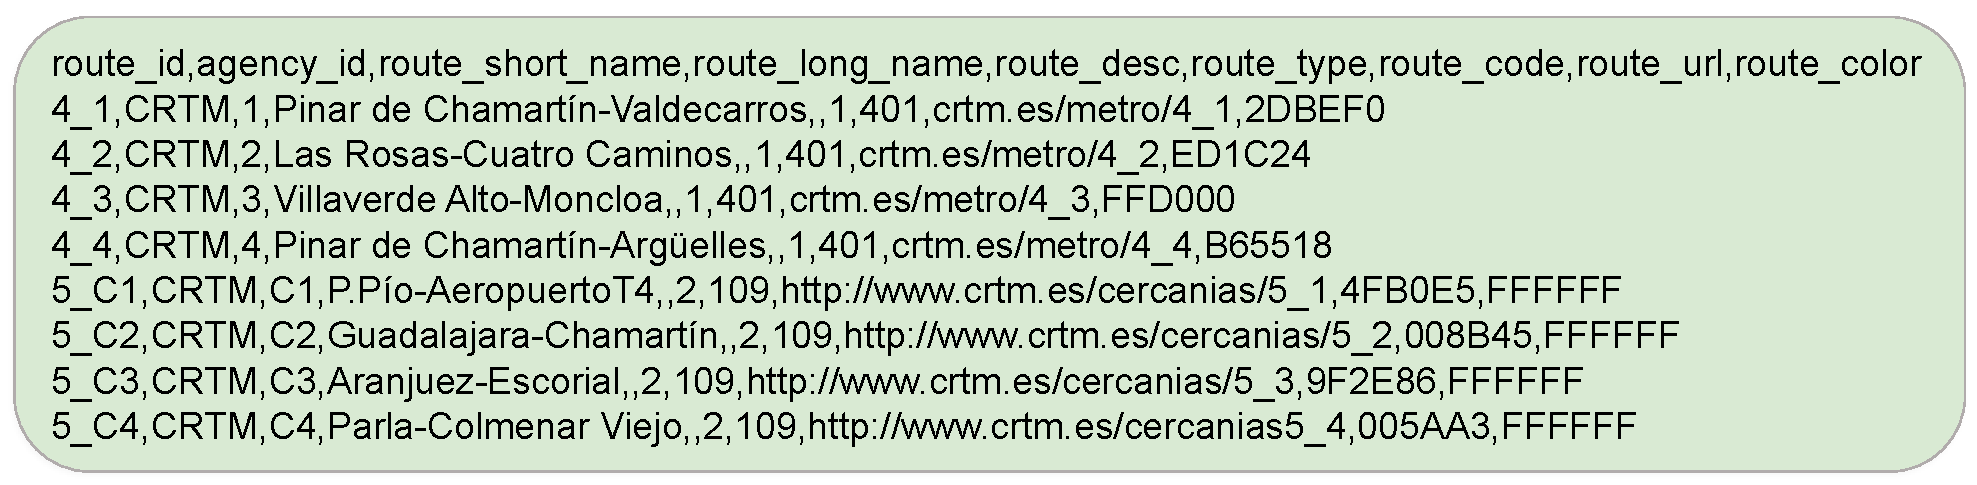
\includegraphics[width=0.5\linewidth]{figures/steps/pushdowninput.pdf} 
    \label{fig:selection2i}
}
\subfloat[Output of routes.csv source.]{
  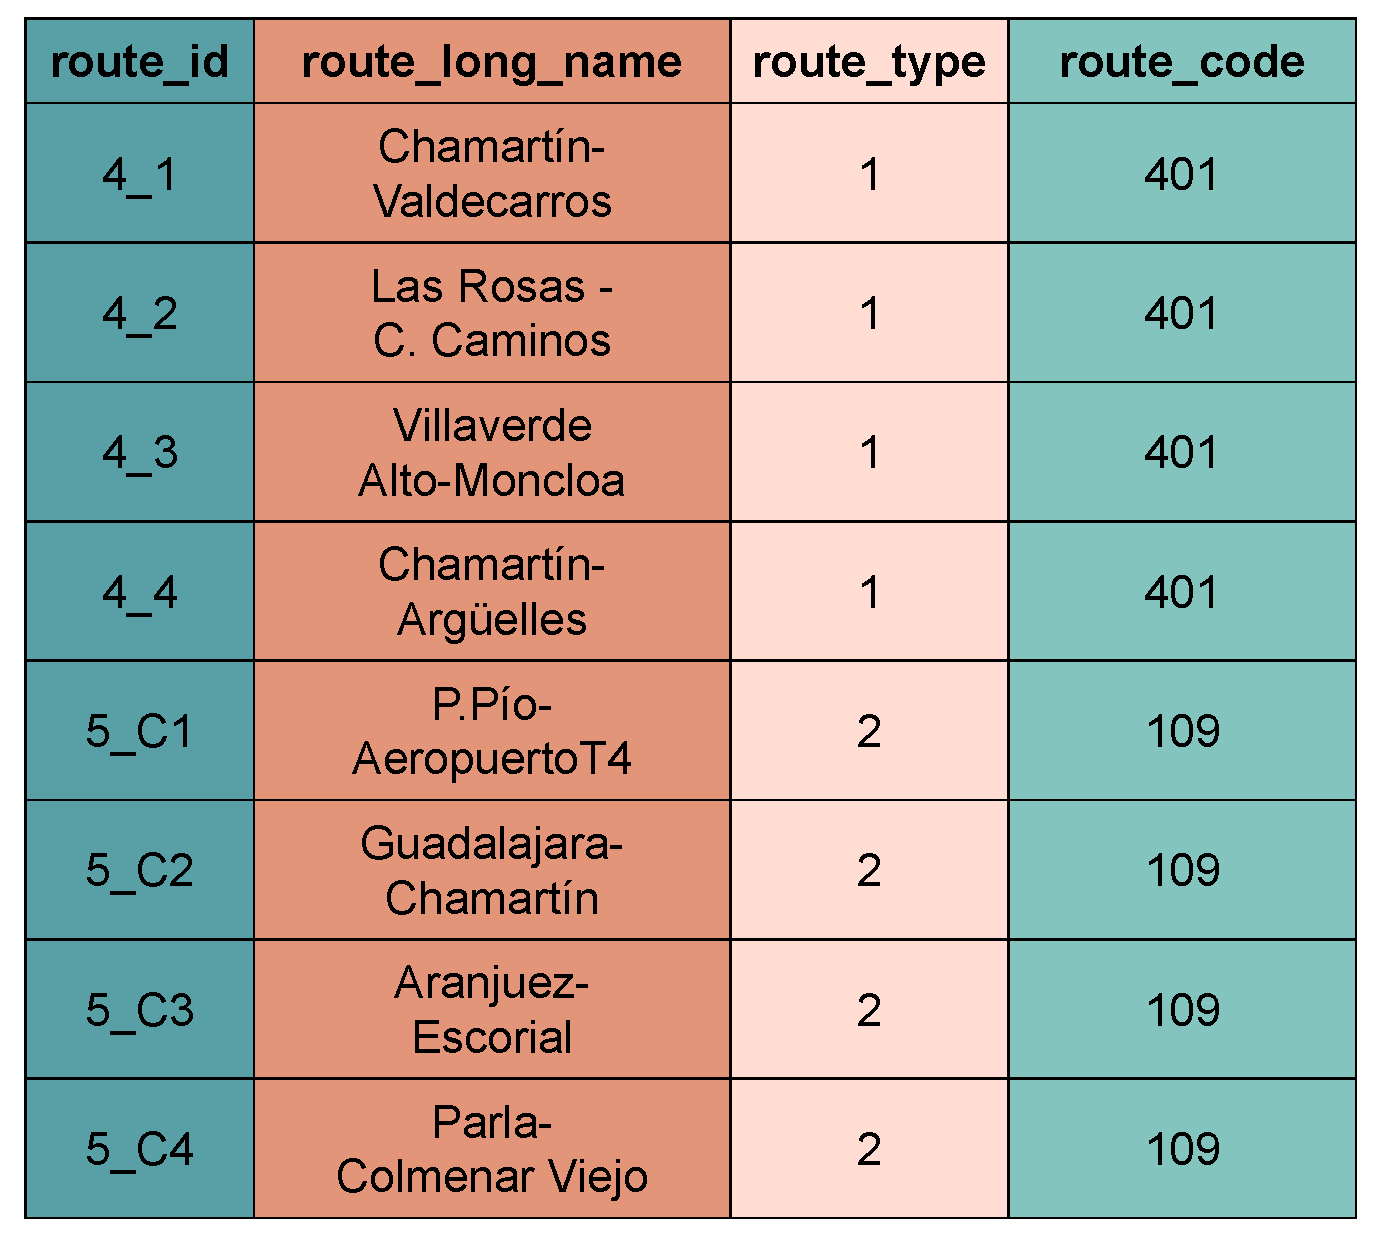
\includegraphics[width=0.5\linewidth]{figures/steps/pushdownresult.pdf}  
  \label{fig:selection2r}
}
\caption[Source selection]{\textbf{Source Selection.} Based on the selection of the rules, only route\_id and trip\_id columns are selected, discarding the rest fields.}
\label{fig:selection2}
\end{figure}

\subsubsection*{Normalization}
There are two functions for performing data normalization. The first one is the treatment of multi-values in a column. In this case, Morph-CSV performs the function $split(A_{ij},sep)$ where $A_{ij}$ is the multi-valued column of source $s_{j}$ and $sep$ is the character defined in the CSVW metadata using the \texttt{csvw:separator} property. The output is a modified $VTD$ with a new source $s_t$ containing the separated values in one column with a common identifier $ID_{ij}$ in another column and an $s_{j}^{'}$ source where the values of $A_{ij}$ are substituted by the identifier defined in $s_t$, $ID_{ij}$. Additionally, this function modifies the mapping document $M$ with a new \texttt{rr:TriplesMap} $TM_t$ generated for the new source $s_t$ and a \texttt{rr:joinCondition} between the \texttt{rr:TriplesMap} of $s_j$, $TM_j$ and $TM_t$. The application of this function is known as the normalization step for second normal form (2NF)~\citep{codd1979extending}. The problems of not performing this step are already mentioned in Section \ref{sec:example}, where the multi-valued columns affect  the query completeness.
 
The second function is the treatment of multiple entities in the same source. Morph-CSV takes the mapping rules and executes the function $cut(\mathcal{M},\mathcal{D}_{tabular})$. This function analyzes the mapping rules $\mathcal{M}$, and performs a 3NF~\citep{codd1979extending} normalization step over ${D}_{tabular}$ when there are two sets of mapping rules ($TM_j$ and $TM_i$) that have the same source, and the intersection of their columns in the rules only contains the join condition references. Following a similar approach as in 2NF, the output is a modified $VTD$ with a set of new sources $s_i\ldots s_n$, each one with the corresponding columns of each entity. For example, in Figure \ref{fig:normalization} we show the 3NF normalization of the \textit{routes.csv} file, that generates an auxiliary source for the \texttt{rr:TriplesMap} with the \textit{gtfs:RouteType} entity data (Figure \ref{fig:normalization}), removing that information from \textit{routes.csv}. In several data integration approaches, normalization steps are not taken into account in order to improve query execution (reducing the number of joins among sources). However, in the case of RDF, where each entity of a class has a unique URI (subject), joins cannot be reduced (see input mapping in Figure \ref{fig:selectionm}). This means that taking into account normalization steps in an OBDA context not only helps to improve query completeness, but also helps to improve performance. Additionally, normalization is also essential for allowing Morph-CSV to efficiently run data preparation steps, as we show in the next step.

\begin{figure}[ht]
\centering
\subfloat[Routes.csv after 3NF normalization step.]{
    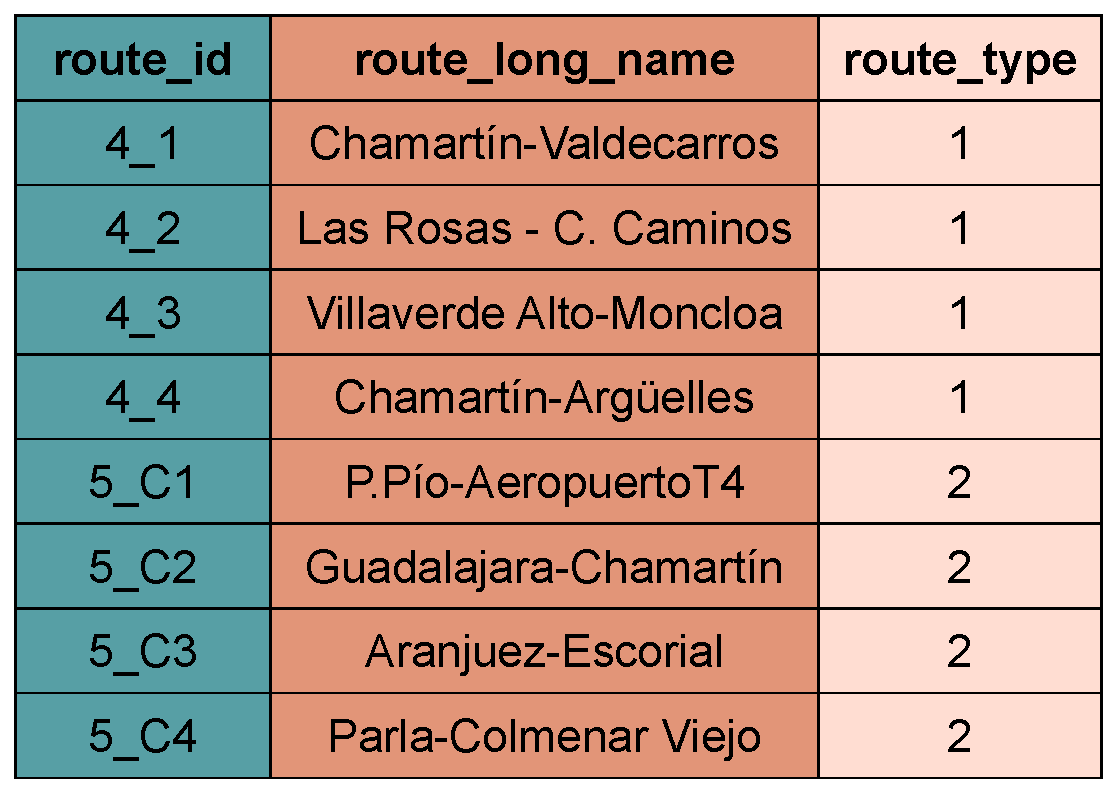
\includegraphics[width=0.5\linewidth]{figures/steps/normalization1.pdf}  
    \label{fig:norm1}
}
\subfloat[Route\_type.csv file generated with Morph-CSV.]{
    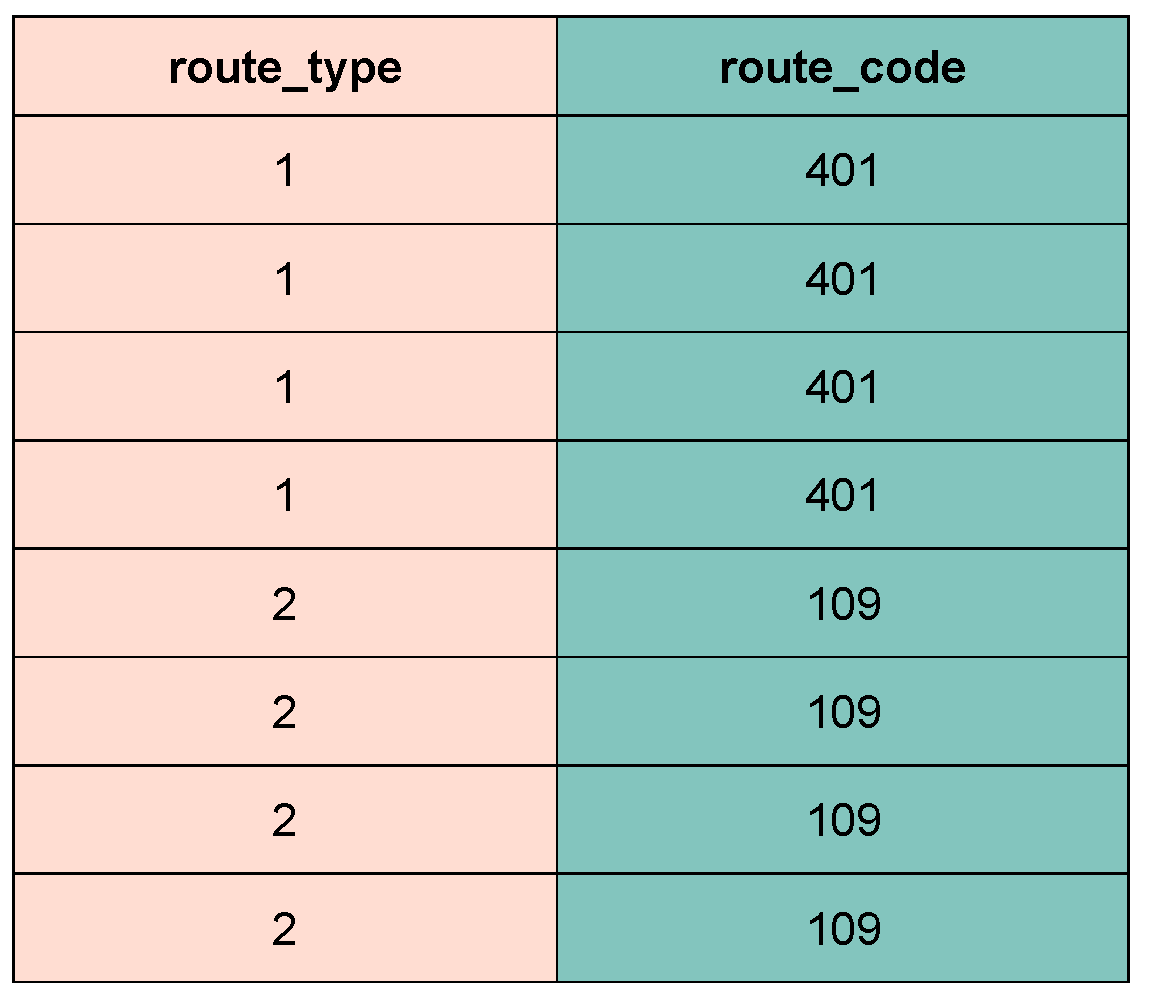
\includegraphics[width=0.5\linewidth]{figures/steps/normalization2.pdf} 
    \label{fig:norm}
}
\caption[Normalization step]{\textbf{Normalization.} 3NF Normalization step over the \textit{routes.csv} file generating other file with the data for \texttt{gtfs:RouteType} class.}
\label{fig:normalization}
\end{figure}

\subsubsection*{Data preparation}
In this step, Morph-CSV addresses the challenge of \textit{Heterogeneity} and executes three different functions: $duplicates$, $sub$ and $create$. First, Morph-CSV removes all duplicates in the raw data, not only the original ones, but also other duplicates that can appear during the normalization step (see Figure \ref{fig:norm}). It applies the ideas described in~\citep{jozashoori2019mapsdi}, performing $duplicates(s_{j})$ where $s_{j}$ is a source in $D_{tabular}$. As it has already been demonstrated in~\citep{jozashoori2019mapsdi,iglesias2020sdm,jozashoori2020funmap}, this step not only has a high impact on the behavior of these engines, but in this case, it also reduces the number of operations performed by Morph-CSV $sub$ and $create$, as they are defined as deterministic functions. The first one is defined as $sub(exp(A_{ij}),val)$ where $exp(A_{ij})$ is a boolean function over column $A_{ij}$ of source $s_{j}$ that when true, the value of $A_{ij}$ is substituted by $val$. There are multiple substitution functions that Morph-CSV executes such as default values, null values and date formats. This function is one of the most important for enhancing the completeness of the query (e.g., enforcing the default values of a column). The second function creates a new column in a specific source $s_{j}$. It is defined as $create(c(A_{nj},\ldots,A_{mj}))$, where $c(A_{nj},\ldots,A_{mj})$ is the application of a set of transformation functions over the columns $A_{nj},\ldots,A_{mj}$ in source $s_{j}$. This function is used to push down the application of ad-hoc transformation functions, usually defined inside the mapping rules~\citep{junior2016funul,de2017declarative}, thus, avoiding the incorporation of them inside the SQL translated query. In Figure \ref{fig:preparation} we show the \textit{route\_type.csv} file after the execution of this step. First, Morph-CSV removes the duplicates of the file obtaining as output a file with only two rows. Then, it executes the transformation function defined in the mapping rules and creates a new column in the file, generating the desired value for the subject of the class according to the LinkedGTFS ontology, ``Subway''. Additionally, the engine substitutes the definition of the transformation functions in the mapping rules by a reference to the created column. In this manner, Morph-CSV efficiently performs the $sub$ and $create$ functions directly over the raw data and together with the normalization step. Thus, the number of joins in the input query is reduced.

\begin{figure}[!ht]
    \centering
    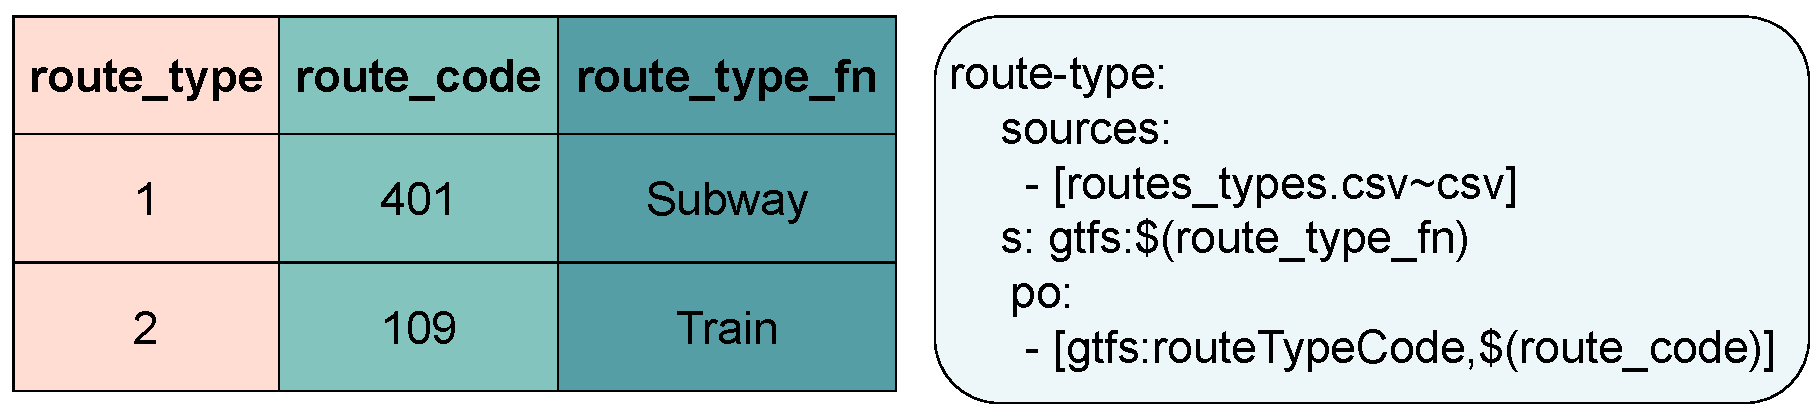
\includegraphics[width=1\linewidth]{figures/steps/creation-result.pdf}
    \caption{Data preparation of \textit{route-types.csv} file.}
    \label{fig:preparation}
\end{figure}

\subsubsection*{Schema creation and load}
The final step before translating and executing the query is the creation of an SQL schema applying the rest of the identified constraints, and loading the selected tabular data sources. Besides the typical integrity constraints that can be extracted from CSVW annotations (PK/FK), Morph-CSV implements a rule for creating indexes in the RDB instance in order to optimize the execution of query joins. In tabular datasets, it is common that the join conditions defined in the mapping rules are based on columns that are not part of PK-FK relations; thus, they are not indexed and OBDA optimizations do not have the desired effect. To address this problem, Morph-CSV gets the \texttt{rr:child} and \texttt{rr:parent} references of the mapping rules and calculates their selectivity on the fly. Then, taking this selectivity into account Morph-CSV decides to create, or not, an index over these columns. Additionally, the mapping document is translated so that it is aligned with the RDB schema that has been created. Figure \ref{fig:rdb} shows the RDB schema generated by Morph-CSV for the input query in Figure \ref{fig:selectionq}, with the applied domain and integrity constraints. 

\begin{figure}[!ht]
    \centering
    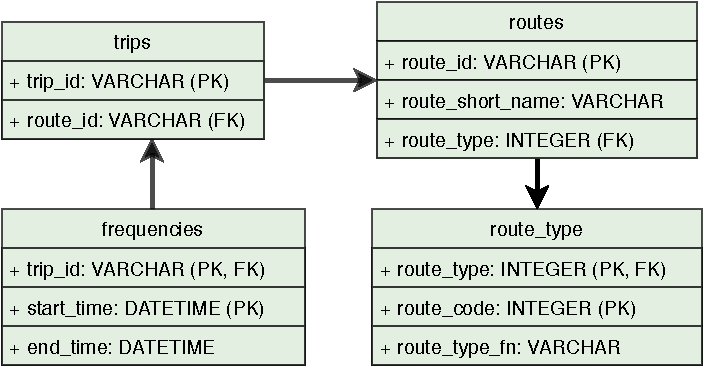
\includegraphics[width=1\linewidth]{figures/steps/rdb.pdf}
    \caption[Output RDB schema from Morph-CSV]{\textbf{Generated schema.} The schema generated by Morph-CSV extracting domain and integrity constraints from the annotations and based on the identified sources selected from the input query.}
    \label{fig:rdb}
\end{figure}


\paragraph{}
There are two main points that make the contributions of Morph-CSV relevant: (i) it incorporates the steps to the standard OBDA workflow without modifying the rest of the steps, hence, it can also benefit from optimizations in other steps of the workflow like query rewriting (reasoning)~\citep{mora2014kyrie2} or query translation (SPARQL-to-SQL)~\citep{priyatna2014formalisation}, and (ii) the reliance of the approach on declarative and standard annotations for OBDA allows the generalization of the proposed steps, usually solved in an ad-hoc manner, not only automatizing the process but also improving its maintainability, understandability and readability.




\subsection{Experimental Evaluation}

This section reports on the results of the empirical evaluation conducted to test the effect of respecting constraints, on the fly, during OBDA query translation over tabular data. The hypothesis we want to validate in our work are:
\begin{itemize}
\item \textit{H1)} The application of a set of domain and integrity constraints over tabular data sources to create an RDB instance that ensures the effectiveness of SPARQL-to-SQL optimizations proposed in the state of the art.
\item \textit{H2)} Extending a common OBDA workflow with a set of additional steps to deal with the challenges for querying tabular data,  does not  impact negatively on the total query execution time.
\item \textit{H3)} The exploitation of declarative and standard annotations in the process of querying tabular data in an OBDA environment, guarantees the independence of the solution and its application over different domains.
\end{itemize}
Aligned with the defined hypothesis, our aim is to answer the following research questions: \textbf{RQ1)} What is the effect of combining different types of constraints over a tabular dataset? \textbf{RQ2)} What is the impact of the constraints when the tabular dataset size increases? \textbf{RQ3)} What is the effect of different kinds of SPARQL query shapes in the extraction and application of constraints?. To answer these questions, we have performed three evaluations in different domains: e-commerce, transportation, and biology. Our first evaluation is in the e-commerce domain, in which we used the Berlin SPARQL Benchmark (BSBM)~\citep{bizer2009berlin}. Our second evaluation is in the transportation domain in which we used the GTFS-Madrid-Bench~\citep{chaves2020gtfs}. This benchmark focuses on measuring the performance of ontology based data access for heterogeneous data sources, based on the publicly-released public transportation data in GTFS format. One of the resources provided by GTFS-Madrid-Bench is a tabular dataset together with its corresponding mappings and annotations together with a set of representative SPARQL queries. Finally, our third evaluation is in the domain of biological data, in which we extend one of our previous proposals~\citep{iglesias2019enhancing} for the generation of an OBDA layer over Bio2RDF tabular datasets. Appendix \ref{apppendix:queries} presents the features of the queries together with the constraints and number of sources used by Morph-CSV. In all of the evaluations the common configurations are:

\noindent\textbf{Engines.} The baselines of our study are two open source SPARQL-to-SQL OBDA engines: Ontop\footnote{\url{https://github.com/ontop/ontop}}$^,$\footnote{We modified the default configuration of Ontop extending the maximum used memory from 512Mg to 8Gb} v3.0.1 and Morph-RDB v3.9.15\footnote{\url{https://github.com/oeg-upm/morph-rdb}}. We select these two engines as they are open source engines (others such as Ultrawrap~\citep{sequeda2013ultrawrap} are not openly available) and also the ones that incorporate the set of most relevant optimizations in the SPARQL-to-SQL query translation process~\citep{priyatna2014formalisation,rodriguez2015efficient}.  To evaluate the baseline approach, we manually generate the relational database schemes of each benchmark without any kind of constraints, and measure the load and query execution times. In order to measure the impact of the additional steps proposed by Morph-CSV\footnote{\url{https://doi.org/10.5281/zenodo.3731941}}$^,$\footnote{\url{https://github.com/oeg-upm/morph-csv}}, we integrate our solution on top of the two OBDA engines in two different configuration: Morph-CSV$^-$ that does not include the source selection step, hence, it loads and applies all the constraints over the input data source each time a query has to be answered, and Morph-CSV that implements the full proposed workflow\footnote{We name the combined engines as follows: a) Morph-CSV: Morph-CSV+Morph-RDB, and Morph-CSV+Ontop; b) Morph-CSV$^-$: Morph-CSV$^-$+Morph-RDB, and Morph-CSV$^-$+Ontop}. To ensure the reproducibility of the experiments, we also provide all of the resources in a docker image.

\noindent\textbf{Metrics.} We measure the loading time of each query and the total query execution time (including the steps proposed by Morph-CSV or baseline when appropriate), and the number of answers obtained (see Appendix \ref{appendix:completeness}). Additionally, we detail the times of each proposed step of our workflow in the execution of each query using Morph-CSV in both configurations (see Appendix \ref{appendix:loadingtime}) following the recommendations proposed in the GTFS-Madrid-Bench~\citep{chaves2020gtfs}. Each query was executed 5 times with a timeout of 1 hour in cold mode, that means that the corresponding database is generated each time a query is going to be evaluated in order to ensure up to date number of answers. Regarding the completeness of the queries, both BSBM benchmark and GTFS-Madrid-Bench provide an RDF materialized version of the input sources that has been loaded in a triplestore (Virtuoso in the case) and used as gold standard. To analyze the completeness of each query, we compare the cardinality of the result set of each configuration against the gold standard assuming its correctness. In the case of the Bio2RDF use case, we cannot compare our results with any gold standard as the last dump version of the project~\citep{dumontier2014bio2rdf} is not comparable with the current status of the input sources, as we declare in one of our previous works~\citep{iglesias2019enhancing}. The experiments were run in an Intel(R) Xeon(R) equipped with a CPU E5-2603 v3 @ 1.60GHz 20 cores, 64GB memory and with the O.S. Ubuntu 16.04LTS.



\subsubsection{BSBM}
The Berlin SPARQL Benchmark~\citep{bizer2009berlin} is one the most popular benchmarks in the Semantic Web field that not only tests the performance of RDF triple stores, but also tests approaches that perform SPARQL-to-SQL query translations providing an RDB instance. It is the chosen benchmark to test the capabilities of many state-of-the-art OBDA engines~\citep{priyatna2014formalisation,calvanese2017ontop,mami2019squerall}. 
 
\begin{figure}[!ht]
  \centering
  \subfloat[Loading time for BSBM 45K.]{
  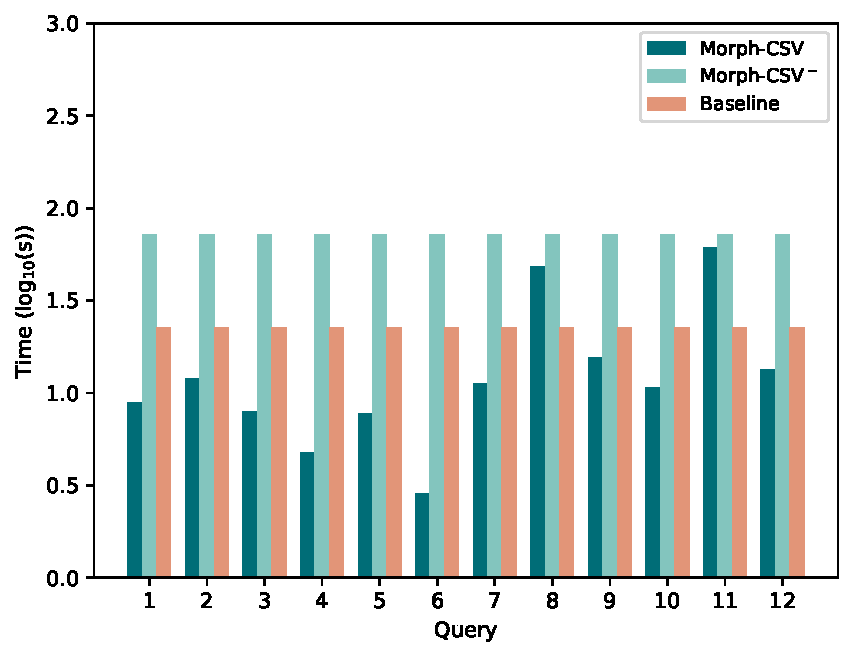
\includegraphics[width=0.48\linewidth]{figures/bsbm/carga_bsbm_45.pdf}
  \label{fig:bsbmload45}
  }
  \subfloat[Loading time for BSBM 90K.]{
  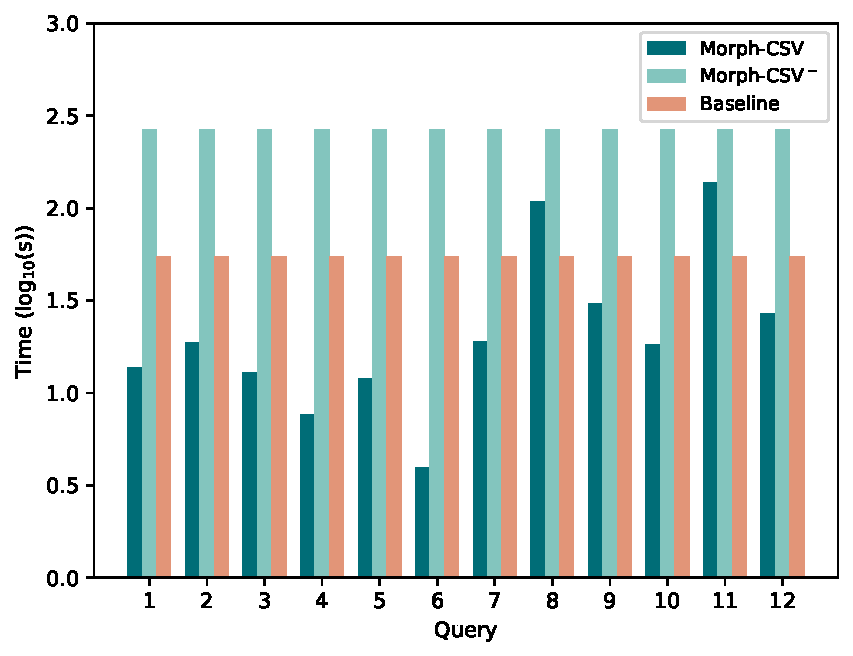
\includegraphics[width=0.48\linewidth]{figures/bsbm/carga_bsbm_90.pdf}  
  \label{fig:bsbmload90}
  }
  \qquad
  \subfloat[Loading time for BSBM 180K.]{
  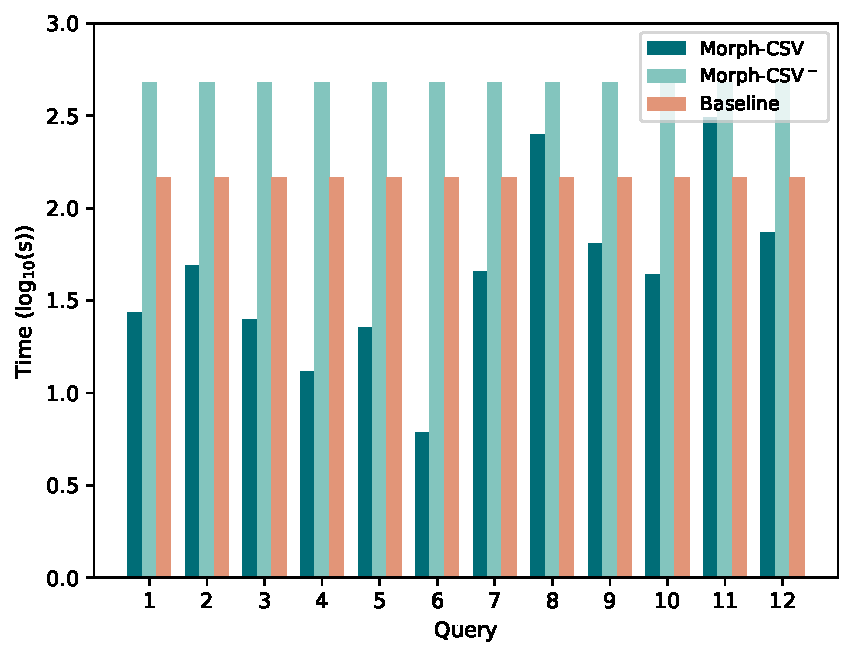
\includegraphics[width=0.48\linewidth]{figures/bsbm/carga_bsbm_180.pdf}  
  \label{fig:bsbmload180}
  }
  \subfloat[Loading time for BSBM 360K.]{
  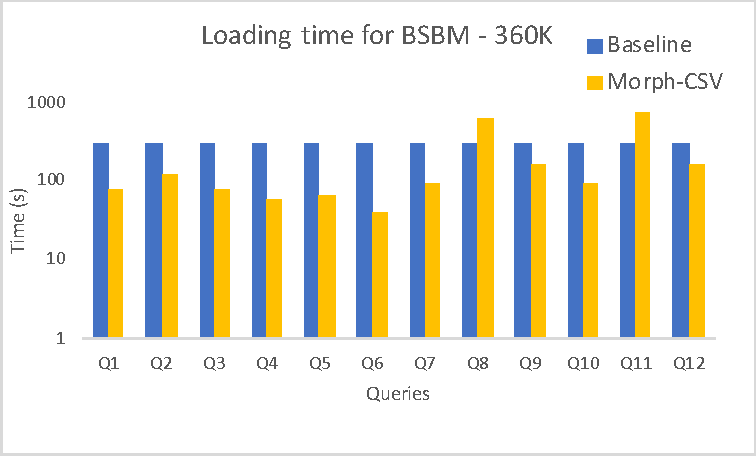
\includegraphics[width=0.48\linewidth]{figures/bsbm/carga_bsbm_360.pdf}
  \label{fig:bsbmload360}
  }
\caption[Loading Time of Tabular Datasets in BSBM.]{\textbf{Loading Time of Tabular Datasets in BSBM.}  Loading time in seconds of the tabular datasets from the BSBM benchmark with number of products 45K, 90K, 180K and 360K. The baseline approach (red columns) and Morph-CSV$^-$ (light green) are constant for each dataset and query, while Morph-CSV (dark green) depends on the query and number of constraints to be applied over the selected sources.}
\label{fig:bsbmload}
\end{figure}


\begin{figure}[!ht]

  \centering
  \subfloat[Total query execution time for BSBM-45.]{
  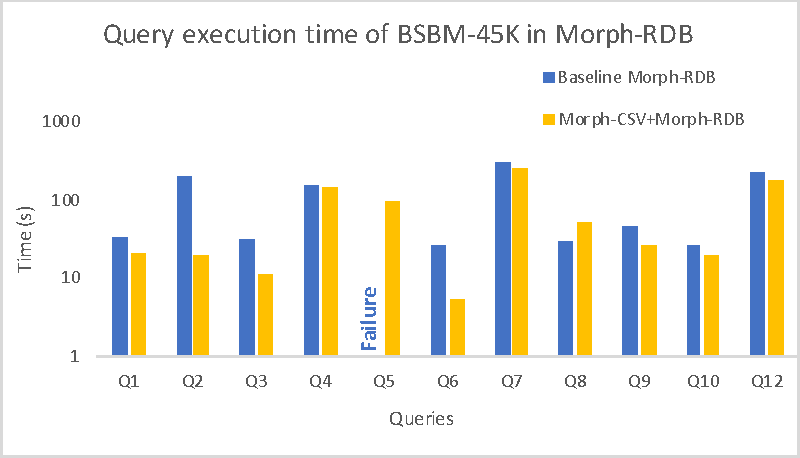
\includegraphics[width=0.48\linewidth]{figures/bsbm/execution_bsbm_morph_45.pdf}  
  \label{fig:morphbsbm45}
  }
  \subfloat[Total query execution time for BSBM-90.]{
  \includegraphics[width=0.48\linewidth]{figures/bsbm/execution_bsbm_morph_90.pdf}  
  \label{fig:morphbsbm90}
  }
  \qquad
  \subfloat[Total query execution time for BSBM-180.]{
  \includegraphics[width=0.48\linewidth]{figures/bsbm/execution_bsbm_morph_180.pdf}  
  \label{fig:morphbsbm180}
  }
  \subfloat[Total query execution time for BSBM-360.]{
  \includegraphics[width=0.48\linewidth]{figures/bsbm/execution_bsbm_morph_360.pdf}
  \label{fig:morphbsbm360}
  }
\caption[Query execution Time in BSBM with Morph-RDB]{\textbf{Query execution Time of Tabular Datasets in BSBM with Morph-RDB.} Execution time in seconds of the tabular datasets from the BSBM benchmark with scale values 45K, 90K, 180K and 360K. The baseline Morph-RDB approach (red columns) is compared with the combination of Morph-CSV (dark green) and Morph-CSV$^-$ (light green) together with Morph-RDB.}
\label{fig:morphbsbm}
\end{figure}


\begin{figure}[!ht]
  \centering
  \subfloat[Total query execution time for BSBM-45.]{
  \includegraphics[width=0.48\linewidth]{figures/bsbm/execution_bsbm_ontop_45.pdf}  
  \label{fig:ontopbsbm45}
  }
  \subfloat[Total query execution time for BSBM-90.]{
  \includegraphics[width=0.48\linewidth]{figures/bsbm/execution_bsbm_ontop_90.pdf}  
  \label{fig:ontopbsbm90}
  }
  \qquad
  \subfloat[Total query execution time for BSBM-180.]{
  \includegraphics[width=0.48\linewidth]{figures/bsbm/execution_bsbm_ontop_180.pdf}  
  \label{fig:ontopbsbm180}
  }
  \subfloat[Total query execution time for BSBM-360.]{
  \includegraphics[width=0.48\linewidth]{figures/bsbm/execution_bsbm_ontop_360.pdf}
  \label{fig:ontopbsbm360}
  }
\caption[Query execution Time in BSBM with Ontop]{\textbf{Query execution Time of Tabular Datasets in BSBM with Ontop.} Execution time in seconds of the tabular datasets from the BSBM benchmark with scale values 45K, 90K, 180K and 360K. The baseline Ontop approach (red columns) is compared with the combination of Morph-CSV (dark green) and Morph-CSV$^-$ (light green) together with Ontop.}
\label{fig:ontopbsbm}
\end{figure}

 
\noindent\textbf{Datasets, annotations and queries.} In order to test our proposal we decided to adapt BSBM, extracting the tabular data sources in CSV format from the SQL generated instances. Additionally, we create the corresponding mapping rules in RML and the metadata following the CSVW specification. We measure the loading time of the two proposals (baseline and Morph-CSV) for each query in the benchmark. Since the focus of Morph-CSV is not the improvement of the support of SPARQL features in the query translation process, we only select the queries of the benchmark that include the supported features  by each engine. This means that Morph-RDB will be evaluated over the queries  Q1, Q2, Q3, Q4, Q5, Q6, Q7, Q8, Q9, Q10 and Q12  and Ontop will be evaluated over Q1, Q3, Q4, Q5 and Q10, both of them using the corresponding R2RML mapping document. For the baseline approach we manually create the RDB schema without  constraints.



\noindent\paragraph*{\textit{BSBM Results}}

\noindent\paragraph*{\textit{Loading Time}.}
The results of the load time for each query and dataset size are shown in Figure \ref{fig:bsbmload}. The main difference between baseline and Morph-CSV$^-$ in comparison with Morph-CSV is that while the loading time for the first two methods is constant for each size, Morph-CSV loading time depends on several input parameters such as the query and the number and type of constraints. In the case of Morph-CSV, it could be understandable that the application of a set of constraints over the raw data in order to improve query performance and completeness, would have a negative impact in the loading time. This happens in queries Q8 and Q11, where the number of sources and the application of the constraints (mainly integrity constraints),  impact negatively on the loading time of the data in the RDB instance in comparison with the baseline approach. However, in the rest of the queries, the Morph-CSV steps focus on the selection of constraints, sources and columns, and on exploiting the information in query and mapping rules, improving the loading time for each query in comparison with the baseline loading time. This means that, although the engine is including a set of additional steps during the starting phase of an OBDA system, the application of these steps only over the data that is required to answer the query, has a positive impact in the total query execution time. Additionally, we can observe that Morph-CSV is able to process, apply the different constraints, and generate the corresponding instance of the RDB for any query. In the case of Morph-CSV$^-$, applying all the constraints defined for the whole dataset each time a query has to be answered, has a negative impact in the loading time, obtaining the worst results in the loading phase.

\noindent\paragraph*{\textit{Evaluation Time with Morph-RDB}.} The query execution time using Morph-RDB as the back-end OBDA engine is shown in Figure \ref{fig:morphbsbm}. The first remarkable observation can be seen in query Q5. Although this query contains features supported by Morph-RDB, the engine reports an error when evaluating the query over the database generated by the baseline approach, because it is not able to evaluate the arithmetic expressions in the FILTER clauses. On the contrary, the datatype of each column in the database generated by Morph-CSV (and also Morph-CSV$^-$) is properly defined, making it possible for Morph-RDB to evaluate the query without any problem and obtaining the expected results. Another remarkable difference is in query Q2, which contains a large number of joins, Morph-RDB reports a timeout error for 180K and 360K with the database generated by the baseline approach. However, it is still able to evaluate this query in reasonable time over the databases generated by Morph-CSV and Morph-CSV$^-$. The effect of the application of integrity constraints in the generation of the RDB instance can also be seen in most of the queries (i.e., Q1, Q2, Q3, Q6, Q9, Q10) reducing considerably the query execution time in the database generated by Morph-CSV in comparison with the baseline approach. There are cases (i.e., Q4, Q7, Q12) where the amount of data to retrieve is large, minimizing the effect of the optimizations. Finally, there are cases where optimizations over the indexes cannot be applied (e.g. querying all the properties of a class). We observe this behavior in Q8, in which the difference between the Morph-CSV+Morph-RDB and Morph-RDB approaches is minimal and this behavior is consistent in all size of datasets. In general, Morph-CSV$^-$ obtains worse results than Morph-CSV+Morph-RDB and Morph-RDB alone. The results are understandable as this configuration has to invest time in preparing the full RDB instance for each query, executing many unnecessary steps in comparison with Morph-CSV. However, in some cases the evaluation time is better than the one obtained over the Morph-RDB configuration, where clearly the creation of indexes and integrity constraints play a key role in the performance of the query execution (see Q2).

\noindent\paragraph*{\textit{Evaluation Time with Ontop}.}
The query execution time using Ontop as the back-end OBDA engine is shown in Figure \ref{fig:ontopbsbm}. Like Morph-RDB, Ontop needs the Morph-CSV generated databases to be able to evaluate Q5 due to the arithmetic expressions of its FILTER operators. Additionally, it also fails in Q10 because it cannot process a FILTER with a date value. In the rest of the queries (Q1, Q3, Q4) we can see that the query evaluation time in Ontop with Morph-CSV is lower than the query evaluation time over the baseline database. Note that in larger databases (180K and 360K), Q1 and Q4 can only be evaluated over the databases generated by Morph-CSV. The Morph-CSV$^-$ configuration is also able to answer the queries just as the Morph-CSV standard configuration, but in comparison with this configuration, the performance is being affected due the inclusion of the additional and unnecessary steps.

As mentioned in the Ontop repository page\footnote{\url{https://github.com/ontop/ontop/wiki/MappingDesignTips}}, integrity constraints are essential for the correct behavior of the engine. Although it is out of the scope of this paper, we observe in our experiments that the main reason why Ontop is only able to answer half of the queries in this benchmark, is related to some issues about maintaining the desirable properties~\citep{corcho2020towards} when translating R2RML mapping rules to its own mappings, called OBDA. The engine also fails to evaluate queries with OPTIONAL clauses when there are NULL values in the answers, as they acknowledged, it is possible that this support has not been implemented in the engine~\citep{xiao2018efficient}.

\noindent\paragraph*{\textit{Query completeness.}} In Table \ref{tab:completeness-bsbm} we show the query completeness obtained with the BSBM benchmark. It is important to remark that our intention to use this benchmark is for testing performance capabilities of our proposals, the input sources are extracted from the BSBM relational model, which is a well formed and normalized RDB instance. However, there are still some cases where we identify the need of applying constraints over the relational database, which are Q5 in the evaluation over Morph-RDB and Q5 and Q10 over Ontop. In these cases, the baseline configurations of the engines are not able to answer those queries, not because they do not support a feature of the SPARQL query or  cannot do it on time, but because they cannot perform the correct comparison among different datatypes in the relational database instance. We demonstrate  with the application of Morph-CSV that queries can be answered and  the correct number of results can be obtained. Additionally, thanks to the application of indexes and integrity constraints there are some queries such as Q1 and Q2 that can be answered by Morph-CSV configuration but not by the baseline, which means that thanks to these steps we are ensuring the effectiveness of the optimizations provided by Ontop and Morph-RDB in the SPARQL-to-SQL translation process. 

\begin{figure}[!ht]
  \centering
  \subfloat[Loading time for GTFS-1.]{
  \includegraphics[width=0.48\linewidth]{figures/gtfs/carga_gtfs_1.pdf}  
  \label{fig:gtfsload1}
  }
  \subfloat[Loading time for GTFS-10.]{
  \includegraphics[width=0.48\linewidth]{figures/gtfs/carga_gtfs_10.pdf}  
  \label{fig:gtfsload10}
  }
  \qquad
  \subfloat[Loading time for GTFS-100.]{
  \includegraphics[width=0.48\linewidth]{figures/gtfs/carga_gtfs_100.pdf}  
  \label{fig:gtfsload100}
  }
  \subfloat[Loading time for GTFS-1000.]{
  \includegraphics[width=0.48\linewidth]{figures/gtfs/carga_gtfs_1000.pdf}
  \label{fig:gtfsload1000}
  }
\caption[Loading Time of Tabular Datasets in GTFS]{\textbf{Loading Time of Tabular Datasets in GTFS.} Loading time in seconds of the tabular datasets from the Madrid-GTFS-Bench with scale values 1, 10, 100 and 1000. The baseline approach (red columns) and Morph-CSV$^-$ (light green) are constant for each dataset and query, while Morph-CSV (dark green) depends on the query and number of constraints to be applied over the selected sources.}
\label{fig:gtfsload}
\end{figure}



\begin{figure}[!ht]
  \centering
  \subfloat[Total query execution time for GTFS-1.]{
  \includegraphics[width=0.48\linewidth]{figures/gtfs/execution_gtfs_morph_1.pdf}  
  \label{fig:morphgtfs1}
  }
  \subfloat[Total query execution time for GTFS-10.]{
  \includegraphics[width=0.48\linewidth]{figures/gtfs/execution_gtfs_morph_10.pdf}  
  \label{fig:morphgtfs10}
  }
  \qquad
  \subfloat[Total query execution time for GTFS-100.]{
  \includegraphics[width=0.48\linewidth]{figures/gtfs/execution_gtfs_morph_100.pdf}  
  \label{fig:morphgtfs100}
  }
  \subfloat[Total query execution time for GTFS-1000.]{
  \includegraphics[width=0.48\linewidth]{figures/gtfs/execution_gtfs_morph_1000.pdf}
  \label{fig:morphgtfs1000}
  }
\caption[Query execution Time in GTFS with Morph-RDB]{\textbf{Query execution Time of Tabular Datasets in GTFS with Morph-RDB.} Execution time in seconds of the tabular datasets from the Madrid-GTFS-Bench with scale values 1, 10, 100 and 1000.  The baseline Morph-RDB approach (red columns) is compared with the combination of Morph-CSV (dark green) and Morph-CSV$^-$ (light green) together with Morph-RDB.}
\label{fig:morphgtfs}
\end{figure}

\begin{figure}[!ht]

  \centering
  \subfloat[Total query execution time for GTFS-1.]{
  \includegraphics[width=0.48\linewidth]{figures/gtfs/execution_gtfs_ontop_1.pdf}  
  \label{fig:ontop1}
  }
  \subfloat[Total query execution time for GTFS-10.]{
  \includegraphics[width=0.48\linewidth]{figures/gtfs/execution_gtfs_ontop_10.pdf}  
  \label{fig:ontop10}
  }
  \qquad
  \subfloat[Total query execution time for GTFS-100.]{
  \includegraphics[width=0.48\linewidth]{figures/gtfs/execution_gtfs_ontop_100.pdf}  
  \label{fig:ontop100}
  }
  \subfloat[Total query execution time for GTFS-1000.]{  
  \includegraphics[width=0.48\linewidth]{figures/gtfs/execution_gtfs_ontop_1000.pdf}
  \label{fig:ontop1000}
  }
\caption[Query execution Time in GTFS with Ontop]{\textbf{Query execution Time of Tabular Datasets in GTFS with Ontop.} Execution time in seconds of the tabular datasets from the Madrid-GTFS-Bench with scale values 1, 10, 100 and 1000. The baseline Ontop approach (red columns) is compared with the combination of Morph-CSV (dark green) and Morph-CSV$^-$ (light green) together with Ontop.}
\label{fig:ontopgtfs}
\end{figure}



\subsubsection{GTFS-Madrid-Bench}
The GTFS-Madrid Benchmark~\citep{chaves2020gtfs} consists of an ontology, an initial dataset of the metro system of Madrid following the GTFS model, a set of mappings in several specifications, a set of queries according to the ontology that cover relevant features of the SPARQL query language, and a data scaler based on a state of the art proposal~\citep{lanti2014npd}. 

\noindent\textbf{Datasets, annotations and queries.} We select the tabular sources of this benchmark (i.e., the CSV files) and we scale up the original data in several instances (scale factors 10, 100 and 1000). Each generated dataset is denoted as GTFS-$S$ where S is the scale factor. The resources of the benchmark already include the necessary mapping rules and tabular metadata. Like our previous evaluation with BSBM benchmark, we only select the queries with features that are supported by each engine: Morph-RDB will be evaluated using  queries Q1, Q2, Q4, Q6, Q7, Q9, Q12, Q13, Q14, Q17 and Ontop will be evaluated using  queries Q1, Q2, Q3, Q4, Q5, Q7, Q9, Q13, Q14, Q17. The description and features of each query are also available online\footnote{\url{https://github.com/oeg-upm/gtfs-bench/}}.

\noindent\paragraph*{\textbf{Madrid-GTFS-Bench Results}}

\noindent\paragraph*{\textit{Loading Time}.}
The loading time of the GTFS-Madrid-Bench queries is shown in Figure \ref{fig:gtfsload}. For GTFS-1 the baseline approach clearly has better performance than Morph-CSV. However, when the size of the datasets increases, the positive effects of applying constraints become more apparent. For most of the queries, the loading time needed by Morph-CSV is lower in comparison to the loading time in the baseline approach. Additionally, similarly to BSBM, there are a set of queries where the application of integrity constraints has a negative impact on the loading time (queries Q1 and Q9). The impact of the application of all of the constraints for answering each query, presented by the configuration Morph-CSV$^-$, clearly impacts over the performance in the loading time.

\noindent\paragraph*{\textit{Evaluation Time with Morph-RDB}.}
The query execution time with Morph-RDB as the back-end OBDA engine is shown in Figure \ref{fig:morphgtfs}. Analyzing the results, we generally observe that the incorporation of Morph-CSV in the workflow of OBDA enhances query performance. With respect to the results of each query, we can observe that on the one hand the behavior of the engine over simple queries (Q1, Q2, Q7, Q12 and Q17) is similar. This is understandable as the selected data sources needed to answer the query do not include the application of several constraints (e.g. there are no joins in the query). On the other hand, in the case of complex queries such as Q4, Q6, Q9, Q13 and Q14, where several tabular sources are needed to answer the queries, the application of constraints has a better impact in comparison to the the baseline approach. Similar behavior is shown over Morph-CSV$^-$, where the complexity of the GTFS data model, with many sources, columns and relations among them, has a clear impact on the total execution time of each query, obtaining worse performance than the baseline in most of the cases. However, for example, in the case of query Q9, Morph-RDB is not able to evaluate the query over the 10th scale database generated by the baseline approach, while in the case of the database generated by Morph-CSV and Morph-CSV$^-$, the query can be answered in reasonable time. In general, due the complexity of GTFS model, we can observe that for small datasets (GTFS-1), the cost of applying the proposed steps of Morph-CSV impacts total execution time. However, when the size of the dataset increases, the baseline approach is impacted due to the fact that it has to load all of the input data sources in the RDB before executing the query, low performance is reported for GTFS-100 and GTFS-1000, including timeout in some queries of the latter. Thanks to the application of the constraints and to the source selection step, for Morph-CSV together with Morph-RDB, the return of the results of the queries has a high performance most of the time. In the cases where Morph-CSV reports a timeout (e.g., Q1 in GTFS-1000); it is because the extremely high number of obtained results cannot be handle by Morph-RDB.

\noindent\paragraph*{\textit{Evaluation Time with Ontop}.}
The experimental evaluation of the query execution in Ontop as the back-end OBDA engine is shown in Figure \ref{fig:ontopgtfs}. This engine is more strict with datatypes in the RDB in comparison with Morph-RDB, and it is why Q2, Q5, Q7 and Q9 produce a failure in the execution over the databases generated by the baseline approach. All these queries have a FILTER clause on a specific datatype (e.g., date, integer, etc) and Ontop proceeds to check the domain constraints before executing the queries. Morph-CSV solves this problem by exploiting the annotations from the metadata and defines the correct datatypes of each column before evaluating the query. For the queries that can be answered by both approaches (Q1, Q3, Q4, Q13, Q14, Q17), the absence of integrity constraints has a negative impact in Ontop, resulting in lower execution time over the databases generated by Morph-CSV. However, similar to the evaluation over Morph-RDB, the complexity of the GTFS data model with a larque quantity of domain and integrity constraints to be applied over the whole dataset, makes that the behavior observed over Morph-CSV$^-$ is being impacted, hence, obtaining worse results that Morph-CSV configuration and the baseline in most of the cases. Finally, in the case where Ontop is not able to evaluate the query under the defined threshold, we report it as a timeout.

\noindent\paragraph*{\textit{Query completeness.}} In the same manner as BSBM benchmark, the focus of the GTFS-Madrid-Bench is on testing the performance and scalability issues of virtual OBDA and OBDI engines. The input dataset is also well formed and normalized. The completeness results of the evaluation are shown in Table \ref{tab:complete-gtfs}, where as we describe before, Morph-RDB has a mechanism to infer the datatypes of the database using the \textit{rr:dataType} annotation from R2RML, which allows  the engine to answer the queries of this benchmark without the need of applying  datatype constraints over the RDB instance. However, Ontop does not include such a mechanism and it needs the declaration of the correct datatypes over the RDB instance, which has a negative impact in the execution of many queries of the benchmark, that cannot be answered using the baseline database but they retrieve the correct results including Morph-CSV (or Morph-CSV$^-$) in the pipeline.

\begin{figure}[!ht]
    \centering
    \subfloat[\textbf{Query execution Time of Tabular Datasets in Bio2RDF with Morph-RDB.} Execution time in seconds of the tabular datasets from  Bio2RDF of Morph-CSV and Morph-CSV$^-$ using Morph-RDB as back-end engine. The baseline is not reported as the loading over the RDB instance reports an error.]{
    \includegraphics[width=0.48\linewidth]{figures/bio2rdf/execution_bio2rdf_morph.pdf}
    }
    \subfloat[\textbf{Query execution Time of Tabular Datasets in Bio2RDF with Ontop.} Execution time in seconds of the tabular datasets from  Bio2RDF of Morph-CSV and Morph-CSV$^-$ using Ontop as back-end engine. The baseline is not reported as the loading over the RDB instance reports an error.]{
    \label{fig:bio2rdfmoprh}
    \includegraphics[width=0.48\linewidth]{figures/bio2rdf/execution_bio2rdf_ontop.pdf}
    \label{fig:bio2rdfontop}
    }
    \caption[Query execution Time of Tabular Datasets in Bio2RDF]{Query execution Time of Tabular Datasets in Bio2RDF}
\end{figure}


\subsubsection{Use Case: The Bio2RDF project}
Bio2RDF is one of the most popular projects that integrates and publishes biomedical datasets as Linked Data~\citep{belleau2008bio2rdf}. Its community has actively contributed to the generation of those datasets using ad-hoc programming scripts, such as PHP. In our previous work~\citep{iglesias2019enhancing} we proposed an alternative way of generating the datasets using a set of declarative mapping rules to improve the maintainability, readability and understanding of the procedure. In comparison with the other benchmarks where the focus of the evaluation was the improvement of the query evaluation time, this real use case contains multiple heterogeneity challenges that, for example, enforce the application of ad-hoc transformation functions (i.e., mappings in the form of RML+FnO). Thus, with this use case we want to demonstrate the benefits of exploiting declarative annotations (metadata and mappings) over the raw data in order to improve query completeness and the need of incorporating the proposed steps for executing queries over real world data sources.

\noindent\textbf{Dataset, annotations, and queries.} Tabular datasets in  CSV or Excel formats cover over 35\% of the total datasets in the Bio2RDF project~\citep{iglesias2019enhancing}. In order to test the capabilities of Morph-CSV, we select a subset of the tabular datasets guaranteeing that they cover all of the identified challenges. Additionally, as far as we are aware, there is no standard benchmark over the Bio2RDF project; we also propose a set of SPARQL queries in order to exploit the selected data. Their main features are shown in Appendix \ref{apppendix:queries}). 


\noindent\paragraph*{\textbf{Bio2RDF Results}}
The results obtained for query evaluation in Bio2RDF are shown in Figure \ref{fig:bio2rdfmoprh} with Morph-RDB as back-end engine and in Figure \ref{fig:bio2rdfontop} with Ontop. The detailed results obtained by Morph-CSV and Morph-CSV$^-$ are shown in Table \ref{tab:bio2rdfdeatiledresults} and the completeness in Table \ref{tab:completness-bio2rdf}. Analyzing the obtained results, we can observe that there are no results for the baseline approach, this means it was not possible to create an RDB schema and load the input data manually. The main reasons are the heterogeneity problems of a real use case that do not exist in the previous evaluations. GTFS and BSBM have well formed and standard source data models. Problems such as the absence of column names, multiple formats of same datatype in different files (numbers, dates) and the use of delimiters inside the column data, make it impossible to generate the baseline approach without a manual and ad-hoc pre-processing step. However, exploiting declarative annotations, Morph-CSV is able to apply the proposed workflow to this dataset, and successfully answer the proposed queries with both back-end OBDA engines. Similar to the previous benchmarks, loading the complete dataset for answering the input query (Morph-CSV$^-$ configuration) has an negative impact on the total execution time. We can observe that for the proposed queries, most of the total evaluation time of each query is spent in the loading process, as the total execution time in Morph-CSV$^-$ is pretty similar for all the queries. Contrary, query execution is benefited by this previous step obtaining the results in reasonable time for all of the queries. 


\subsection{Discussion of Experimental Results}
\label{sec:discussion}
We have run an experimental evaluation to analyze what are the effects on the use of declarative annotations to extract and apply constraints to enhance virtual OBDA approaches. We have tested our approach over three different cases: (i) a well known benchmark (BSBM) from the e-commerce domain; (ii) a benchmark focused on a virtual OBDA approach for the transport domain; and (iii) a real use case from the biological domain. We describe the main conclusions and findings based on the results obtained:
\begin{itemize}
    \item \textbf{Query complexity:} Clear benefits are obtained from being able to analyze and take advantage of the information provided by the input query, before translating and running it. It allows to only select sources and constraints that are going to be useful for answering the query, avoiding carrying out additional and unnecessary functions over the raw data. Together with the mapping rules, the queries are essential to make relevant decisions during the on-the-fly physical design of the RDB instance (e.g., integrity constraints). Approaches such as the Morph-CSV$^-$ configuration can be valuable when the freshness of the results is not a main requirement, for example to perform a materialization process, which will ensure high quality RDF files where the domain constraints have been applied.
    \item \textbf{Data size:} The total query evaluation time is being impact from how the engine manages the input dataset and the application of constraints. The delegation of these operations to the RDBMS system after loading the full dataset may not be efficient enough. Morph-CSV pushes down the source selection and the application of domain constraints over the raw data. Although it incorporates a set of additional steps in comparison with the baseline, the benefits in the query execution time by the SPARQL-to-SQL engine are already demonstrated, enhancing the total execution time of the queries in most of the cases.
    \item \textbf{Declarative annotations:} The use of declarative and standard mapping rules and metadata makes it possible the generalization of the proposal, avoiding ad-hoc and manual steps. It also incorporates a set of important benefits for the process such as the improvement of its maintainability, readability, and understandability.
    \item \textbf{Querying raw data in OBDA:} Most of the data shared on the web is currently raw data in well known formats such as CSV, JSON, and XML. Semantic Web and more specifically, OBDA technologies, play a key role in starting to see the web as an integrated  database that can be queried. With this approach, we demonstrate that querying tabular data is: i) neither a trivial nor an easy task that can be delegated to na\"ive querying approaches and ii) optimizations and improvements can still be proposed taking advantage and exploiting current annotation proposals to not only enhance performance but also completeness.
\end{itemize}





\section{Morph-GraphQL: GraphQL Server Generation from Declarative Mappings}
\label{chap6_morphgraphql}
Introduced in 2000, Representational State Transfer (REST) has become the most common manner to provide web services in the last decade. Those web services that conform to the REST principles, known as RESTful web services, use HTTP/S and its operations to make requests to the underlying server, such as GET to retrieve objects, POST to add objects, PUT to modify objects and DELETE to remove objects, among others.

Over the years, the complexity of modern software concept has evolved since the inception of REST. For example, typical mobile applications have to take into account aspects that receive little attention in traditional applications, such as the size of data being exchanged/transmitted and the number of API calls being made. These aspects are relevant to the problem known as \textit{over-fetching} and \textit{under-fetching}~\citep{bryant2017graphql,vogel2017experiences,mukhiya2019graphql}. Over-fetching refers to the situation in which a REST endpoint returns more data than what is required by the developer~\citep{bryant2017graphql,vogel2017experiences,mukhiya2019graphql}. For example, a developer may need some information about the name of a user, so she hits the corresponding endpoint (\texttt{/user}). However, the endpoint may return information that is not needed by the client, such as birth date and address. The opposite also raises a problem, which is having the REST endpoint provide less data than required. Such a case is called under-fetching~\citep{bryant2017graphql,vogel2017experiences,mukhiya2019graphql}. It refers to the situation in which a single REST endpoint does not provide sufficient information requested by the client. For example, in order to obtain the names of all friends of a particular user, typically two endpoints may be needed: the first is the endpoint that returns the identifiers of all the friends (\texttt{/friends}), and the second is the one that returns the details of each of the friends based on the identifier (\texttt{/user}).

In order to ameliorate the aforementioned problems, Facebook proposed the GraphQL query language \citep{graphql}, initially being used internally by the company in 2012. GraphQL was released for public use in 2015 and since then has been adopted by companies from various sectors such as technology (GitHub), entertainment (Netflix), finance (PayPal), travel (KLM), among others. 

Two main components of a GraphQL server are \textbf{schema} and \textbf{resolvers}.
The GraphQL schema specifies the type of an object together with the fields that can be queried. GraphQL resolvers are data extraction functions responsible for accessing the underlying datasets. These functions are written by software engineers using a  specific programming language and, are then used by GraphQL engines, which translate GraphQL queries to the corresponding underlying query language of the sources (e.g., SQL). Multiple GraphQL engines support major programming languages (e.g. JavaScript, Python, Java, Golang, Ruby). In addition to the aforementioned frameworks, query planning tools have been developed in order to translate GraphQL queries into other query languages (e.g. dataloader\footnote{\url{https://github.com/facebook/dataloader}}, joinmonster\footnote{\url{https://join-monster.readthedocs.io/en/latest/}}).

Generating a GraphQL server requires expertise from both domain experts and software developers. Typically, the following tasks need to be done: 
\begin{enumerate}
    \item A domain expert would analyse the underlying datasets, propose a unified view schema as a GraphQL schema and how the source datasets would need to be mapped into the GraphQL schema. Note that there is no standard mechanism to represent these mappings. Domain experts may use a spreadsheet, which is not necessarily easy to understand by another domain expert. In the absence of a standard representation, different ways to represent mappings are possible. Some of such spreadsheets represent the relation among source and target concepts in a na\"ive manner using. Others use Excel files with pages, such that each page represents a concept. Others add ids instead of property names.
    It becomes even more messy when there is an operation involved (e.g. source has the name in two properties/columns, ``first-name'' and ``last-name'' while the target has one single attribute to represent both, ``name'').
    \item A software developer would then implement those mappings as GraphQL resolvers, a process that takes significant resources. Given that the complexity of any given source code grows faster than the size of the source code, generating GraphQL resolvers would become more difficult even for a standard-sized dataset which typically contains more than a handful tables and hundreds of properties. This situation might worsen if the underlying dataset evolves, considering that the corresponding resolvers have to be updated as well. GraphQL resolvers may not be easily understood by other developers who were not involved in the initial version, thus bringing the possibility of introducing errors.
\end{enumerate}

In this section, we propose the exploitation of declarative mapping languages to specify the rules that relate the source datasets and the GraphQL schema. Declarative mapping languages, such as the W3C R2RML~\citep{R2RML} and its extensions, have been used to generate knowledge graphs from existing datasets. The use of declarative mappings is based on the idea that a standard mapping language (or such extensions) would facilitate a better understanding of the relationships between the underlying data source and the exposed GraphQL schema. Furthermore, they also allow for better maintainability as those mappings are independent from any programming language. Our main contribution is an approach that translates declarative mappings to GraphQL resolvers. We focus on the feasibility of the approach and leave the soundness, completeness, and complexity analysis for future work.

\subsection{The Morph-GraphQL framework}
The Morph-GraphQL framework (Figure \ref{fig:obda2graphql}) proposes the exploitation of the information encoded in declarative mapping rules following a well-known specification (e.g. R2RML and RML) to generate GraphQL servers. A domain expert can create these types of mappings without the need for programming skills. Despite that the creation of mappings might not be easy for domain experts to be created from scratch, there are several tools with easy to use graphical interface that already developed by researchers in the semantic Web community such as RMLEditor~\citep{heyvaert2016rmleditor} or KARMA~\citep{knoblock2015exploiting}. The generated GraphQL servers benefit from the wide range of tools available for GraphQL in order to access data stored in various formats (i.e. RDB, CSV, JSON). The approach consists of the following steps: 1) the generation of the definition of a query to be evaluated by the underlying dataset (e.g. ListEpisodes), 2) the generation of the types in the GraphQL schema and 3) the generation of GraphQL resolvers. 

\begin{figure}[!ht]
    \centering
    \includegraphics[width=0.8\linewidth]{figures/workflow-morphgraphql.pdf}
    \caption[morph-GraphQL workflow]{\textbf{morph-GraphQL workflow.} morph-GraphQL receives declarative mappings and generates GraphQL servers. These servers, as it is defined in the specification, contain their two main components (i.e. schema and resolvers) that can be used by any GraphQL engine to evaluate queries over the data source.}
    \label{fig:obda2graphql}
\end{figure}



\textbf{Auxiliary Functions}. We present here a set of auxiliary functions that will be used in the functions that generate resolvers.
\begin{itemize}
    \item $getConstant(TermMap)$ takes the constant \texttt{prefix:attr} in the constant-value term map where $TermMap = \texttt{rr:constant "prefix:attr"}$ and retrieves its specific value $attr$.
    \item $getReference(TermMap)$ retrieves the reference \texttt{ref} in the reference-value term map where $TermMap = \texttt{rr:column "ref"}$ or $TermMap = \texttt{rml:reference "ref"}$.
    \item $getTemplate(TermMap)$ retrieves the template \texttt{template} in the template-value term map where $TermMap = \texttt{rr:template "template"}$. In this case, the function retrieves the concatenation between the strings and the references that are part of the template, hence, the implementation of this functions depend of the underlying query system used for retrieving the data. For example, given an SQL database and the term map \texttt{rr:template "ex.com/episode/\{eid\}"} as the inputs, this function returns \texttt{"ex.com/episode/" || eid} or \texttt{CONCAT("ex.com/episode/\{eid\}", eid)}.%, depending on the database system being used.
    \item $getDataType(ObjectMap)$ that given an \texttt{rr:ObjectMap} that contains a \texttt{rr:dataType "xsd:type"} returns the corresponding GraphQL type. For example, $getDataType(rr:dataType ``xsd:string")$ returns \texttt{String}.
    \item $getTypeFromClass(SubjectMap)$ that given an \texttt{rr:SubjectMap} returns the type value based on the \texttt{rr:class} property. For example, $getDataType(rr:class ``foaf:Person")$ returns \texttt{Person}. 
\end{itemize}

\subsubsection{Generating Queries} 
We present a set of translation functions that convert a triples map into the corresponding query to be used in GraphQL resolvers. This set of functions is adapted from the work presented in \citep{chebotko2009semantics}, originally proposed to translate SPARQL queries into SQL queries without the presence of any mappings. 
\begin{itemize}
    \item $\alpha(TriplesMap)$ returns a set of logical sources associated with the triples map $TriplesMap$, which is the logical source associated to the triples map $TriplesMap$ and additionally all the referenced source if $TriplesMap$ contains Referenced Object Maps.
    \item $\beta(TermMap)$ that given a term map $TermMap$ returns the corresponding query expression, that is: 
    \begin{itemize}
        \item $getConstant(TermMap)$ if $TermMap$ is a constant-value map
        \item $getReference(TermMap)$ if $TermMap$ is a reference-value map
        \item $getTemplate(TermMap)$ if $TermMap$ is a template-value map.
    \end{itemize}    
    \item $alias(TermMap)$ generates a unique alias to be used in the query generation.    
    \item $genPR(TriplesMap)$ generates a query expression which projects the relevant query expressions of a triples map $TriplesMap$ (i.e., $\beta$ of Subject Map and all Object Maps) together with their aliases.
    \item $genCond(TriplesMap)$ generates a query expression which is evaluated to true if they match the arguments passed in the resolver functions and additionally the join conditions if $TriplesMap$ contains Referenced Object Maps.
    \item Finally, $trans(TM)$ builds the valid query statement using the results of the previous functions. For example, in the case of an SQL database, \texttt{$trans(TM)$ = "SELECT $genPR(TM)$ FROM $\alpha(TM)$ WHERE $genCond(TM)$"} translates a triples map into the corresponding SQL query.
\end{itemize}

\subsubsection{Generating Schema}
The generation of the Schema for GraphQL is divided into two steps. The first one is focused on the generation of the possible entry points of the server (i.e. the query root) and the second one generates the Types defined for the server. Exploiting the mapping rules as inputs, Morph-GraphQL automatically generates both components.

\subsubsection{Generating Query Root}
First, Morph-GraphQL generates the entry points of the server. Algorithm~\ref{algQueryRoot} shows how this step is executed. Taking as input a mapping document, it iterates over the TriplesMap and extracts the information needed for defining the entry points: the type value extracted from the class property of the subject map and the set of attributes together with the types extracted from the predicate-object maps. Morph-GraphQL is able to generate automatically a set of basic entry points (e.g. ListEpisodes, ListCharacter) that can be filtered by each attribute.
\begin{algorithm}
%\footnotesize
\caption{GenerateQueryRoot(Mapping)}
\label{algQueryRoot}
\begin{algorithmic}
\STATE $queryRoot.init()$
\FORALL{$TriplesMap \leftarrow Mapping$}
    \STATE $typeClass = getTypeFromClass(TriplesMap.getSubjectMap())$
    \STATE $poms = TriplesMap.getPredicateObjectMaps()$
    \FORALL{$pom \leftarrow poms$}
      \STATE $datatype = getDataType(pom.getObjectMap())$
      \STATE $attribute = getConstant(pom.getPredicateMap())$   
      \STATE $attributes.add(attribute,datatype)$
    \ENDFOR
    \STATE $query = createListQuery(typeClass,attributes)$
    \STATE $queryRoot.add(query)$
\ENDFOR
\RETURN $queryRoot$ 
\end{algorithmic}
\end{algorithm}


\subsubsection{Generating Types}
Algorithm \ref{algGenerateSchema} generates a GraphQL type from a Triples Map. It generates a GraphQL type $typeClass$, where $typeClass$ is the class specified in the Subject Map of the Triples Map. The fields of the $typeClass$ are all the mapped predicates in the Predicate Object Maps of the Triples Map. The datatypes of the fields are the results of function $getDataType$, which returns the corresponding GraphQL type from the datatype specified in the Object Maps of the Triples Map. This function is called for each TriplesMap defined in the mapping document.

\begin{algorithm}
%\footnotesize
\caption{GenerateType(TriplesMap)}
\label{algGenerateSchema}
\begin{algorithmic}
\STATE $type.init()$
\STATE $typeClass = getTypeFromClass(TriplesMap.getSubjectMap())$
\STATE $type.add(typeClass)$ 
\STATE $poms = TriplesMap.getPredicateObjectMaps()$
\FORALL{$pom \leftarrow poms$}
  \STATE $datatype = getDataType(pom.getObjectMap())$
  \STATE $attribute = getConstant(pom.getPredicateMap())$
  \STATE $type.add(createAtttribute(attribute, datatype))$
\ENDFOR
\RETURN $type$
\end{algorithmic}
\end{algorithm}


\subsection{Generating Resolvers}
%TBD see Listing \ref{lstGenerateQueryRootResolver}.
%\lstinputlisting[
%frame=single
%, basicstyle=\footnotesize
%, numbers=left
%, label=lstGenerateQueryRootResolver
%, caption=Function generateQueryRootResolver
%, xleftmargin=2em, xrightmargin=2em
%, language=JavaScript
%]{listings/lstGenerateQueryRootResolver.tex}



Algorithm \ref{algGenerateQueryRootNaive} generates a GraphQL resolver from a TriplesMap. Based on the entry points defined in the schema, for each TripleMap, Morph-GraphQL generates the \texttt{list$typeClass$} resolver. First, it defines the function for querying the Type $typeClass$ with the attributes defined in the mapping. Then, the algorithm use the function ($trans$ function) to translate the query to the underlying query language adapting the approach defined in~\citep{chebotko2009semantics}. These two steps use the auxiliary functions $getRereference()$ and $getTemplate()$ in order to obtain the correct references of the data source columns/keys from the mapping rules. Finally, defines the manner how the engines has to executes the query on the underlying database engine and generates the corresponding instances by calling the constructor of Type $typeClass$.

\begin{algorithm}
%\footnotesize
\caption{GenerateResvolver(TriplesMap)}
\label{algGenerateQueryRootNaive}
\begin{algorithmic}[1]
\STATE $resolver.init()$
\STATE $typeClass = getTypeFromClass(TriplesMap.getSubjectMap())$
\STATE $poms = TriplesMap.getPredicateObjectMaps()$
\FORALL{$pom \leftarrow poms$}
  \STATE $attribute = getConstant(pom.getPredicateMap())$
  \STATE $attributes.add(attribute)$
\ENDFOR

\STATE $resolver.add(defineListQueryFunction(typeClass,attributes))$
\STATE $resolver.add(translateQuery(trans(TriplesMap))$
\STATE $resolver.add(execute(query,rdb))$
\STATE $resolver.add(constructResults(attributes,queryResults))$
\RETURN $Resolver$


\end{algorithmic}
\end{algorithm}


\subsection{Morph-GraphQL}
In this section, we present the experimental evaluation of Morph-GraphQL. Our aim is to answer the following questions:
\begin{itemize}
    \item \textbf{RQ1:} Can Morph-GraphQL generate a GraphQL server from declarative mappings that is able to answer the set of queries provided by a GraphQL benchmark?
    \item \textbf{RQ2:} Is there any significant difference between for the queries that can be answered by the generated GraphQL server in terms of response time between GraphQL queries and their equivalent SPARQL queries posed over the RDF dataset generated by the same declarative mappings?
\end{itemize}

We have implemented our framework as an open-source project \textbf{Morph-GraphQL}\footnote{\url{https://github.com/oeg-upm/morph-graphql}}$^,$\footnote{\url{https://doi.org/10.5281/zenodo.3584339}}. In our previous work~\citep{priyatna2019morph} we described the full example of Star Wars generating a GraphQL server based on an R2RML mapping using Morph-GraphQL. Currently, the Morph-GraphQL framework is able to: translate R2RML mappings into a Javascript-based GraphQL server for accessing tabular datasets (CSV files or Relational Databases)\citep{priyatna2019morph}. We use the JoinMonster library\footnote{\url{https://join-monster.readthedocs.io}} to generate efficient SQL queries when joins are needed.

\subsubsection{Link\"{o}ping GraphQL Benchmark} 
Currently, the only GraphQL benchmark available is the Link\"{o}ping GraphQL Benchmark (LinGBM), proposed by Hartig et al.~\citep{hartig2019LinGBM}. This benchmark focuses on exposing read-only GraphQL APIs over a legacy relational database. At the time of writing, the LinGBM benchmark v1.0 sets its context in the domain of e-commerce. It consists of a dataset generator and a set of query templates (a query with placeholder variables to be instantiated). Additionally, guidelines are provided on the mapping between the relational database schema and the GraphQL schema (e.g. Table Offer is mapped to GraphQL type Offer). 

\textbf{Dataset Generator.}
The dataset generator\footnote{\url{https://github.com/LiUGraphQL/LinGBM/wiki/Datasets}} is based on the Berlin SPARQL Benchmark (BSBM)~\citep{bizer2009berlin}. The dataset contains ten tables (e.g.  Vendor, Offer, Producer, Product, and Person, Review) with different join cardinalities (e.g. 1-1, 1-N, M-N).

\textbf{Choke-points and Queries.} 
The benchmark includes a list of \textit{choke-points}, which are challenges that have been identified for answering GraphQL queries. This is done following the design methodology for benchmark development\footnote{\url{http://ldbcouncil.org/blog/choke-point-based-benchmark-design}} introduced by the Linked Data Benchmark Council\footnote{\url{http://ldbcouncil.org/}}. Five classes of choke-points that are proposed are: 
\begin{enumerate}
    \item Choke Points Related to Attribute Retrieval. (1 check-point)
    \item Choke Points Related to Relationship Traversal. (5 choke-points)
    \item Choke Points Related to Ordering and Paging. (3 choke-points)
    \item Choke Points Related to Searching and Filtering. (5 choke-points)
    \item Choke Points Related to Aggregation. (2 choke-points)
\end{enumerate}

These choke-points are covered in the 16 hand-crafted query templates provided by the benchmark. The summarise of the queries, the relation with the proposed choke-points and the support of Morph-GraphQL is show in Table \ref{table:supported-queries}.


\begin{figure}[ht]
    \centering
    \includegraphics[width=.8\linewidth]{figures/evaluation.pdf}
    \caption[Morph-GraphQL evaluation workflow.]{\textbf{Evaluation Workflow.} We evaluated Morph-GraphQL by comparing its performance over the supported LinGBM queries againts two equivalent Semantic Web approaches. First one is the materialisation of the LinGBM RDB to RDF using R2RML mappings and the second one is the translation from SPARQL-to-SQL using also the the same mapping rules.}
    \label{fig:eval-workflow}
\end{figure}

\subsubsection{Evaluation Setup}
\begin{table}[!ht]
 \centering
  \caption[Morph-GraphQL supported LinGBM queries]{Supported Queries in Morph-GraphQL}
 \label{table:supported-queries}
  \begin{tabular}{c | c | c} 
  \toprule
   Query & Choke Points & Morph-GraphQL Support  \\
 \midrule
  Q1 & 1.1, 2.1, 2.2 & Yes   \\ 
  Q2 & 2.1 & Yes  \\
  Q3 & 2.2, 2.3 & Yes   \\
  Q4 & 2.2, 2.3, 2.5 & Yes  \\
  Q5 & 2.1, 2.2, 2.3, 2.4 & Yes  \\ 
  Q6 & 2.2, 2.5 & Yes   \\ 
  Q7 & 2.2, 2.5, 3.2 & No    \\ 
  Q8 & 3.1, 3.3 & No    \\ 
  Q9 & 2.1, 2.2, 3.1, 3.3 & No    \\ 
  Q10 & 1.1, 4.1 & No   \\ 
  Q11 & 2.5, 4.4 & No   \\ 
  Q12 & 2.5, 4.3 & No   \\ 
  Q13 & 2.1, 4.2, 4.3 & No   \\ 
  Q14 & 2.1, 4.2, 4.3, 4.5 & No   \\ 
  Q15 & 5.2 & No   \\ 
  Q16 & 5.1 & No   \\ 
  \bottomrule
  \end{tabular}
 
 \end{table}
We used the LinGBM Data Generator to generate the various sizes of datasets\footnote{The size is defined in terms of number of products in the database (1K means 1 thousand products)} (1K, 2K, 4K, 8K, 16K, 32K, 64K and 128K) and loaded them in the relational database. We created declarative mappings following the mapping guidelines provided in the benchmark. For each query template, we generated 20 queries with different instances generated randomly, as it is the default settings of the benchmark. To measure the performance, we run each query instance 5 times in cold mode, and we calculate the average for each query. We also generated the equivalent SPARQL queries that are to be evaluated over a knowledge graph. The knowledge graph is generated by Morph-RDB \citep{priyatna2014formalisation} from the datasets using the same declarative mappings. 
All the resources used in the evaluation is available online on our GitHub repository\footnote{\url{https://github.com/oeg-upm/morph-graphql/}}.
Figure~\ref{fig:eval-workflow} illustrates the evaluation workflow explained above. The figure shows a materialised and virtualised knowledge graphs. The materialised knowledge graph is the data transformed to RDF and stored into virtuoso ``LinGBM Knowledge Graph'' (a triple store to store knowledge graph data).
The virtualised view does not transform the original datasets to another format (the data is stored in a RDB). It provides access to the underlying datasets via GraphQL. Once a GraphQL query is received, the GraphQL server uses GraphQL engine to translate the query into SQL, which would query the Database ``LinGBM RDB'', get the results, and then the results of the SQL query will be changed into the requested format according to the GraphQL query. We measure the total query execution time for:
\begin{itemize}
    \item GraphQL queries that are translated into SQL queries and evaluated in a relational database instance database. We use Morph-GraphQL v1.0.0 to evaluate these queries.
    \item SPARQL queries that are evaluated over the materialised knowledge graph that is, queries are evaluated using a triple store. We use a Virtuoso v7.2.5.1 instance in this case.
    \item SPARQL queries that are evaluated over the virtual knowledge graph that is, queries are translated into SQL queries and evaluated by Morph-RDB v3.9.15 over the relational database instance. 
\end{itemize}
The experiments were run in an Intel(R) Xeon(R) equipped with a CPU E5-2603 v3 @ 1.60GHz 20 cores, 100G memory with Ubuntu 16.04LTS.

\subsubsection{Results and Discussion}

\begin{table}[]
\centering
\caption[Query execution time of Morph-GraphQL]{Query evaluation performance (time in seconds) over multiple sizes of the LinGBM (the number indicates the scale factor used). Execution time is a lower-is-better metric.}
\label{tab:results}
\resizebox{0.9\textwidth}{!}{%
\begin{tabular}{l|c|c|c|c|c|c|c}
\hline
\multicolumn{1}{c|}{\textbf{Engine/Queries}} & \textbf{Q1} & \textbf{Q2} & \textbf{Q3} & \textbf{Q4} & \textbf{Q5} & \textbf{Q6} & \textbf{\begin{tabular}[c]{@{}c@{}}Geometric\\  Mean\end{tabular}} \\ \hline
\multicolumn{8}{c}{\textbf{LinkGBM 1K}}                              \\ \hline
Morph-GraphQL & 0.103 & 0.146 & 0.005 & 0.118 & 0.237  & 0.079 & 0.075 \\ \hline
Morph-RDB     & 0.168 & 0.081 & 0.201 & 0.221 & 0.296  & 0.089 & 0.159 \\ \hline
Virtuoso      & 0.182 & 0.017 & 0.091 & 0.079 & 1.204  & 0.131 & 0.124 \\ \hline
\multicolumn{8}{c}{\textbf{LinkGBM 2K}}                              \\ \hline
Morph-GraphQL & 0.183 & 0.200 & 0.006 & 0.171 & 0.397  & 0.071 & 0.100   \\ \hline
Morph-RDB     & 0.167 & 0.085 & 0.203 & 0.224 & 0.308  & 0.088 & 0.161 \\ \hline
Virtuoso      & 0.096 & 0.025 & 0.057 & 0.068 & 1.291  & 0.073 & 0.098 \\ \hline
\multicolumn{8}{c}{\textbf{LinkGBM 4K}}                              \\ \hline
Morph-GraphQL & 0.314 & 0.316 & 0.005 & 0.311 & 0.799  & 0.096 & 0.151 \\ \hline
Morph-RDB     & 0.171 & 0.083 & 0.199 & 0.223 & 0.318  & 0.089 & 0.161 \\ \hline
Virtuoso      & 0.109 & 0.035 & 0.059 & 0.078 & 12.293 & 0.101 & 0.167 \\ \hline
\multicolumn{8}{c}{\textbf{LinkGBM 8K}}                              \\ \hline
Morph-GraphQL & 0.597 & 0.644 & 0.004 & 0.625 & 1.363  & 0.096 & 0.228 \\ \hline
Morph-RDB     & 0.178 & 0.080 & 0.196 & 0.225 & 0.323  & 0.090 & 0.162 \\ \hline
Virtuoso      & 0.096 & 0.070 & 0.064 & 0.069 & 2.142  & 0.097 & 0.135 \\ \hline
\multicolumn{8}{c}{\textbf{LinkGBM 16K}}                             \\ \hline
Morph-GraphQL & 1.121 & 1.408 & 0.005 & 1.293 & 2.776  & 0.104 & 0.376 \\ \hline
Morph-RDB     & 0.167 & 0.083 & 0.205 & 0.222 & 0.322  & 0.089 & 0.162 \\ \hline
Virtuoso      & 0.100 & 0.122 & 0.057 & 0.073 & 1.412  & 0.090 & 0.137 \\ \hline
\multicolumn{8}{c}{\textbf{LinkGBM 32K}}                             \\ \hline
Morph-GraphQL & 2.635 & 2.884 & 0.005 & 2.543 & 6.086  & 0.130 & 0.644 \\ \hline
Morph-RDB     & 0.173 & 0.085 & 0.199 & 0.220 & 0.323  & 0.089 & 0.163 \\ \hline
Virtuoso      & 0.108 & 0.274 & 0.069 & 0.085 & 1.591  & 0.122 & 0.179 \\ \hline
\multicolumn{8}{c}{\textbf{LinkGBM 64K}}                             \\ \hline
Morph-GraphQL & 5.157 & 5.940 & 0.005 & 5.114 & 11.065 & 0.147 & 1.050 \\ \hline
Morph-RDB     & 0.177 & 0.085 & 0.199 & 0.224 & 0.325  & 0.090 & 0.164 \\ \hline
Virtuoso      & 0.116 & 0.417 & 0.057 & 0.091 & 1.666  & 0.102 & 0.187 \\ \hline
\multicolumn{8}{c}{\textbf{LinkGBM 128K}}                            \\ \hline
Morph-GraphQL & 8.806 & 9.552 & 0.005 & 8.437 & 22.453 & 0.152 & 1.526 \\ \hline
Morph-RDB     & 0.172 & 0.084 & 0.199 & 0.224 & 0.324  & 0.090 & 0.163 \\ \hline
Virtuoso      & 0.120 & 0.381 & 0.058 & 0.090 & 1.613  & 0.115 & 0.188 \\ \hline
\end{tabular}%
}
\end{table}

In terms of choke-points, Morph-GraphQL supported queries that belong solely to two classes: \textit{attribute retrieval} and \textit{relationship traversal}. Queries which belong to the classes \textit{ordering-and-paging} and \textit{searching-and-filtering} are not supported by Morph-GraphQL. Nonetheless, this can be addressed in a future version of Morph-GraphQL. The last class of chock points addresses \textit{aggregations}, which has not been addressed yet in the GraphQL specification.


We show the results for the different dataset sizes in Table~\ref{tab:results}. We see that for smaller dataset sizes (1K,2K, and 4K), Morph-GraphQL outperforms the others for the majority of the queries. The main reason of these results for smaller dataset sizes is because of the overhead (for translating queries from SPARQL to SQL and optimising the resulting SQL) in Morph-RDB has a negative impact in the total performance of the query execution. Morph-GraphQL needs less time translating the query because it is relatively more simple to translate GraphQL to SQL compared to SPARQL to SQL. In most of the cases for these dataset sizes, Virtuoso needs more time than the other two systems due to the absence of indexes in RDF which has a negative impact depending on the features of the query~\citep{endris2019ontario}. For bigger datasets, SPARQL to SQL optimisations~\citep{priyatna2014formalisation} implemented in Morph-RDB pays off the translation time and gives better impact over the query execution process, outperforming Morph-GraphQL, which hints that the optimisations in the query translation from GraphQL to SQL can still be improved in order to query big datasets (32K, 64K, 128K). When we consider the whole set of queries and calculate the geometric mean of the results, we notice that Morph-GraphQL outperforms the others in some of the dataset sizes because of its fast execution time for the queries Q3 and Q6. Analysing the queries individually, we can observe that for all the engines, Q5 is the most costly one due to the number of nested queries that it consists. 




\chapter{Optimizations for Scaling-up Materialized Knowledge Graph Construction Techniques}
\label{chapter:construction}


In this Chapter we introduce two approaches to optimize the construction of materialized knowledge graphs. Diverse approaches have been proposed to define the process of integrating heterogeneous datasets into knowledge graphs \citep{chebotko2009semantics,calvanese2017ontop,chaves2019what,priyatna2014formalisation}. Mapping languages (e.g., R2RML \citep{R2RML} and RML \citep{dimou2014rml}) and engines (e.g., RMLMapper\footnote{\url{https://github.com/RMLio/rmlmapper-java}} and RocketRML \citep{csimcsek2019rocketrml}) represent valuable contributions for performing this transformation process. Albeit highly used, existing approaches lack efficient data management techniques demanded to create knowledge graphs from large and heterogeneous datasets with duplicates. In the same manner as the approaches proposed in Chapter \ref{chapter:virtual}, the two contributions described exploit the information from mapping rules and ideas presented in Chapter \ref{chapter:mappig-translation} to scale-up the construction of KG.

Section \ref{chap7_rdfizer} presents an efficient set of data structures and their corresponding physical operator to scaling up the construction of materialized KGs where the mappings are following the RML specification. We empirically demonstrate the efficiency of the proposal and compare the obtained results against state of the art RML engines such as RocketRML y RMLMapper. Section \ref{chap7_funmap} describes FunMap, a set of optimization techniques for efficiently pre-processing functional mappings (mappings such as RML+FnO, that include transformation functions) and generation of function-free RML mappings that can be used by any RML parser. The two contributions presented in this Chapter are joint collaborations with the Scientific Data Management Group from TIB research center.



\section{Efficient RML parsing for Knowledge Graph Materialization at Scale}
\label{chap7_rdfizer}
Knowledge graphs have gained momentum as data structures to integrate--as factual statements-- data and knowledge present in heterogeneous data sources. 
DBpedia and Wikidata are exemplary encyclopedic knowledge graphs frequently accessed by scientific and industrial communities; e.g., only Wikidata receives billions of visits per month\footnote{\url{https://stats.wikimedia.org/}}. 
Similarly, knowledge graphs are receiving significant attention in science and industrial developments \citep{AuerKPKSV18,NoyGJNPT19}. In fact, according to Google, knowledge graph is a trend term\footnote{\url{https://trends.google.com/trends/explore?q=knowledge\%20graph}} and the Google Scholar indexes more than 3,5M entries of scientific publications with the term knowledge graph.
Although results demonstrate the success in the adoption of Semantic Web technologies, put in perspective the need of providing efficient and mature technologies for constructing and maintaining knowledge graphs. 

   


\noindent \textbf{Motivating Example:}
Creating a knowledge graph from biomedical data sources is an exemplary scenario of being overwhelmed by the volume and heterogeneity of data. 
In~\autoref{fig:motivatingExample}, we see a normal process of transforming two real-world data sources into an RDF knowledge graph using an available RML interpreter. 
In this example, the aim is to integrate data related to the biological concept RBP\_RNA\_PhysicalInteraction\footnote{Protein(RBP)-RNA binding interactions are shown to play important roles in diseases.
Although there is a lack of enough experimental data, various computational methods are filling this gap by predicting physical interactions between RBP and target RNAs.} from different sources into RDF. 
Accordingly, the subject of \texttt{TripleMap1} represents the mentioned concept. 
Considering the fact that related data is residing in two different sources, a \textit{Join Condition} is applied in the mapping rules to create the required triples. 
It should be noted that even though only four different attributes of both data sources are utilized, the data volumes are considerably large; about 1 Gigabyte in total. 
In this example, to transform the raw data into RDF, two widely accepted RML-compliant interpreters\footnote{\url{https://github.com/RMLio/rml-implementation-report}}, i.e., RMLMapper\footnote{\url{https://github.com/RMLio/rmlmapper-java}} and RocketRML~\citep{csimcsek2019rocketrml} are executed. 
However, none of the mentioned engines accomplish the task. 
In the case of RocketRML, the process stops early due to failure of the memory capacity. 
While applying RMLMapper, the transformation process times out after 48 hours. 
The inability of available engines to perform in this scenario demonstrates the need to develop engines able to perform complex transformations in an efficient manner.
\\
\begin{figure}[t!]
\centering
\includegraphics[width=0.7\textwidth]{figures/Motivating_Example_v1.1.pdf}
\caption[SDM-RDFizer motivating example]{\textbf{Motivating example.} Available RML engines, implementing naive join strategy, fail to create a KG from two biomedical datasets with a total size of 1GB and 25\% duplicates.} 
\label{fig:motivatingExample}
\end{figure}
\textbf{Our Resource:} We address the problem of efficient knowledge graph creation, and propose a resource named SDM-RDFizer which is able to transform data from myriad data sources into an RDF knowledge graph. SDM-RDFizer implements a set of unique physical operators and data structures that speed up the execution of the mapping rules that specify a knowledge graph creation process. The current version of SDM-RDFizer is customized for RML, a mapping language extensively used for the creation of knowledge graphs in diverse domains~\citep{dimou2014rml}.    
SDM-RDFizer is publicly available as a resource in a Github\footnote{\url{https://github.com/SDM-TIB/SDM-RDFizer}} and in Zenodo\footnote{\url{https://doi.org/10.5281/zenodo.3872103}}. SDM-RDFizer is used in more than eight international projects. Moreover, experimental results reveal the contribution that SDM-RDFizer makes to the repertoire of efficient technologies for knowledge graph management.  
\begin{figure}[t!]
    \centering
    \includegraphics[width=1\textwidth]{figures/architecture_v1.1.jpg}
    \caption[SDM-RDFizer architecture]{The architecture of the SDM-RDFizer.}
    \label{fig:architecture}

\end{figure}



\begin{figure}[h!]
 \centering
 \subfloat[Predicate Tuple Table]{
      \includegraphics[width=0.8\textwidth]{figures/PTT.png}
    \label{fig:ptt}}

  \subfloat[Predicate Join Tuple Table]{
\includegraphics[width=0.8\textwidth]{figures/PJTT.jpg}
    \label{fig:pjtt}}
    \caption[Physical Data Structures for KGC]{{\bf The Physical Data Structures.} The two physical data structures used by SDM-RDFizer are illustrated. (a) A Predicate Tuple Table with three entries. (b) A Predicate Join Tuple Table with two entries.}
    \label{fig:hash_table}
\end{figure}
\subsection{The SDM-RDFizer: An RML Engine}

This section describes the SDM-RDFizer in terms of its architecture, the physical operators that make up the execution engine of RML triples maps, and the main properties of these operators.  

\subsubsection{The SDM-RDFizer Architecture}
A data integration system \textit{DI} provides an abstract representation $\langle O,S,M\rangle$ to specify the mapping rules in a set $M$ that define the integration of a set $S$ of data sources into instances of a unified schema or ontology $O$. 
SDM-RDFizer receives as input a data integration system \textit{DI} and produces as output instances of the concepts in $O$ that result from the execution of the mapping rules in $M$ over the data sources in $S$. 
The current version of SDM-RDFizer is customized for interpreting data integration systems where mapping rules are specified in RML, and the output corresponds to an RDF knowledge graph with the ontology $O$. 
However, the SDM-RDFizer architecture can be easily implemented for other RDF based mapping languages (e.g., R2RML~\citep{R2RML}).  
The execution of the RML triples maps requires the interpretation of triples maps, the creation of physical data structures to store the results of the execution of the RML rules, and the generation of the knowledge graph from the results stored in the data structures. \autoref{fig:architecture} depicts SDM-RDFizer in terms of four main components that implement these steps. 

\noindent\textbf{RML Triples Map Syntax Interpreter:} translates the RML triples maps into the physical data structures that SDM-RDFizer uses to execute the RML triples maps and generate the RDF triples.

\noindent\textbf{RML Operators:} execute the interpreted triples maps over the respective data sources to generate RDF triples. 
During the execution of these operators, the physical data structures are accessed to check if an RDF triple has already been created.
If so, the generation of a duplicated RDF triple is avoided, otherwise, the triple is stored in the physical data structure.
SDM-RDFizer has three operators; they are explained in more detail in \autoref{operators}.
    \begin{itemize}
        \item \textit{Simple Object Map}: is the most basic of the operators to evaluate a \textit{simple predicate object map} statement in an RML triples map. The values of the \textit{object values} are collected from an attribute in the triples map source or are a constant. In the motivating example, this operator generates RDF triples according to the predicate object map in lines 7-9 in \autoref{fig:motivatingExample}.  
        \item \textit{Object Reference Map}: this operator \textit{references a second triples map}. The object of the first triples map is the subject of the second triples map. The main condition for this operator to work is that both triples maps have the same data source. An application of this operator in the motivating example can be seen in lines 11-14. 
        \item \textit{Object Join Map}: this operator executes a \textit{join condition} between two RML triples maps with different data sources. In the motivating example, this operator is utilized to execute the predicate object map in lines 21-25 in \autoref{fig:motivatingExample}.
    \end{itemize}
    
\noindent\textbf{Physical Data Structures:} store results generated so far and avoid the generation of duplicates during the execution of RML triples maps. They are of two types: 
\begin{itemize}
\item i) Predicate Tuple Table (PTT): to store per each of predicate $p$ in at least one triple map, the RDF triples generated for $p$ so far. 
\item ii) Predicate Join Tuple Table (PJTT): to store the values of the subjects generated by a triples map that are associated with the values that meet a join condition in the triples map.  
\end{itemize}
These structures are explained in more detail in \autoref{pds}.

\noindent\textbf{Knowledge Graph Creator:} collects RDF triples stored in PTTs and adds them to the output knowledge graph. The knowledge graph creation is performed incrementally, i.e., as soon as a new RDF triple is added into a PTT, the RDF triple is also included in the knowledge graph. To avoid the same RDF triple to be added more than once, the knowledge graph creator maintains per PTT $t$, the timestamp of the last RDF triple that was selected from $t$. 

\subsubsection{Physical Data Structures}
The SDM-RDFizer utilizes two physical data structures as a means to optimize the creation of knowledge graphs. These data structures help with the removal of duplicates and to avoid unnecessary operations, like uploading the parent triples map's data source of a join multiple times. In the following subsection, the physical data structures used by SDM-RDFizer are described. 
\label{pds}

\noindent\textbf{Predicate Tuple Table (PTT)} 
For each predicate $p$ defined in an object triples map, a PTT is created to store the RDF triples generated so far. Physically, PTTs are implemented as hash tables where the hash key of an entry corresponds to an encoding of the subject and object of a generated RDF triple, and the value of the entry corresponds to the RDF triple. The main use of this table is to avoid the duplicate generation of an RDF triple. 
If a generated RDF triple is present within PTT, that means that the triple has been previously generated, and it needs to be discarded. But if the generated RDF triple is not present within PTT, then it is new and must be added to PTT and to the knowledge graph. As it can be seen in the figure\autoref{fig:ptt}, the data source is transformed into RDF triples which checked in the corresponding PTT. As RDF triples of a predicate $p$ can be generated from the execution of different triples maps, PTTs bring great savings not only in sources with high-duplicated rates but also when data sources that generate RDF triples of $p$ also overlap.  

\noindent
\noindent\textbf{Predicate Join Tuple Table (PJTT)}
A PJTT stores the values generated during the execution of a join condition between two RML triple maps, e.g., lines 21-25 in \autoref{fig:motivatingExample}, the predicate object map is defined in terms of a join of triples map \texttt{TriplesMap1} (child map) to \texttt{TriplesMap2} (parent map). For each RML triples map $M_i$ that is referred as a parent triples map in a join condition $B$, a predicate join tuple table $M_i \_B$ is created, e.g., \texttt{TriplesMap2\_enst} in our running example. 
Physically, predicate join tuples are hash tables. The hash key of an entry corresponds to the encoding of each of the values of the attributes in the condition $B$ (e.g., \texttt{enst}), while the value of the entry is a set with all the subject values generated by $M_i$ (e.g., values of the subject of \texttt{TriplesMap2}) that are associated with the values of the attributes in $B$ represented in the entry hash key.  
 Additionally, a PJTT enables direct access to the subjects associated with the join condition $B$, allowing thus for the join implementation as an index join.  
 In the example shown in Figure\autoref{fig:pjtt}, "enst" is the join condition between the triples maps. The data is organized as the values of the join conditions with its respective value in dataSource2. For example, we have the value "ENST00000415827" and its associated values "ENSE00003628092" and "ENSE00003642731".  In PJTT, "ENST00000415827" is the key in the hash table and "ENSE00003628092" and "ENSE00003642731" are the values. Finally, to identify an entry in PJTT, a key is generated from the identifier of the parent triples map and the join condition.  
\begin{figure}[h!]
 \centering
 \subfloat[Simple Object Map]{
      \includegraphics[width=0.45\textwidth]{figures/Basic_conversion_v1.1.jpg}
    \label{fig:om}}
  \subfloat[Object Reference Map]{
\includegraphics[width=0.45\textwidth]{figures/Mapping_reference_v1.1.jpg}
    \label{fig:orm}}

  \subfloat[Object Join Map]{
\includegraphics[width=0.6\textwidth]{figures/Join_v1.1.jpg}
    \label{fig:ojm}}
    \caption[Efficient Physical operator for KGC]{SDM-RDFizer implements three physical RML operators that rely on PTTs to avoid the generation of duplicates. Object Join Maps resort to PJTTs to provide a direct access to the inner tables (i.e., the parent triples maps) of a join between two triples maps; also, PJTTs avoid the traversal of a parent triples map in case it is referenced by more than one triples map.}
    \label{fig:DTR}
\end{figure}

\subsubsection{RML Operators and Algorithms}
\label{operators}
%Brief Overview
SDM-RDFizer implements three different operators for the creation of knowledge graphs. Depending on the type of the triples map, the SDM-RDFizer executes the respective operator. If the triples map has a join condition, then an \textbf{Object Join Map} operator is used. If the triples map have a reference to another triples map but do not have a join condition, then the \textbf{Object Reference Map} operator is used. Finally, if the triples map does not have a join condition or a reference to another triples map, then the \textbf{Simple Object Map} is used. We now describe the operators in more detail.

\noindent\textbf{Simple Object Map (SOM)}
 It is the most basic operator that SDM-RDFizer can execute and enables the generation of an RDF triple by executing a simple predicate object map statement. As it is illustrated in Figure\autoref{fig:om}, given a triples map and its respective data source, SDM-RDFizer generates RDF triples following what is established in the map. Each generated RDF triple is checked against the corresponding predicate tuple table (\textbf{PTT}). If the generated RDF triple already exists in PTT, then it is discarded. In the opposite case, the RDF triple is added both to PTT and to the knowledge graph. This operation is depicted in Figure\autoref{fig:om} where two RDF triples are generated. "<http://iasis.eu/Q8WU90\_ENST00000415827> <iasis:interactionScore> “0.665”." is not in PTT, then, it is added both to the table and to the knowledge graph.  

\noindent\textbf{Object Reference Map (ORM)}
It seeks to expand what is established in Simple Object Map. By using the subject of a triples map as the object of another triples map. The main condition for this operator to work is that both triples maps have the same data source. Afterwards, the same process as in Simple Object Map is applied on the generated RDF triples, i.e., the triples are checked against PTT to determine if the triples are required for the knowledge graph creation. An example of this operation is in Figure\autoref{fig:orm}. In the figure, there are two triples maps, where the \textit{<TripleMap2>} acts as the parent triples map. Two RDF triples are generated but only the new one is included in the PTT. 

\noindent\textbf{Object Join Map (OJM)}
It seeks to expand what is established in Object Reference Map, but the main difference is that triples maps have different data sources. By using the corresponding PJTT, SDM-RDFizer implements an index join where the outer table of the join corresponds to the values in the child map, and the inner table to the PJTT. Thus, to validate the satisfaction of a join condition $B$, the value of $B$ is checked in PJTT and if an entry $e$ exists with that hash key, all the subjects in $e$ are used to generate the resulting RDF triples. Finally, similar to the last two operations, the generated RDF triples are checked against the corresponding PTT to validate duplication and decide if they are going to be included in the knowledge graph. A way to better understand this operation is to view Figure\autoref{fig:ojm}. In the figure, the join condition is the column "enst" in both data sources. A PJTT table is created from the data associated with the join condition as shown in Figure\autoref{fig:pjtt}. Three RDF triples are generated and only two are not duplicates (i.e., they are not in the PTT). This operation is similar to Object Reference Map, since the object of the triples is the subject of the parent triples map. 
\subsubsection{Properties} 
We present the main properties of the RML operators implemented by SDM-RDFizer. Per operator \texttt{o}, we seek to compare the number of operations done by SDM-RDFizer versus the ones done by a na\"ive implementation of \texttt{o}; we named these expressions $\phi_{\texttt{o}}(.)$ and $\widehat{\phi}_{\texttt{o}}(.)$, respectively. Without lost of generality, we just focus on main-memory operations per operator, i.e., comparisons and insertions in main-memory data structures. Consider a predicate $p$, a multiset $N_p$, and set $S_p$; $N_p$ includes all the RDF triples of $p$ while $S_p$ is the corresponding set of $N_p$. Consider $|N_p|$ and $|S_p|$ as the cardinality of $N_p$ and $S_p$, respectively. In presence of a high-duplicate rate of RDF triples of $p$, $|S_p|$ is much smaller than $|N_p|$ (i.e., $|S_p| \ll|N_p|$).
\begin{itemize}
    \item \textbf{Simple Object Map (SOM):}
    Let $M$ be an RML triples map with an object triples map that defines $p$, $\phi_{\texttt{o}}(M)$ and $\widehat{\phi}_{\texttt{o}}(M)$ are defined as follows.  
  The na\"ive implementation of the simple object map operator $o$ in $M$ generates all the duplicates and then, it needs to execute a duplicate elimination process to add the RDF triples to the knowledge graph. Suppose a merge sort algorithm is conducted to eliminate duplicates \citep{BittonD83}\footnote{$\Theta(.)$ corresponds to the asymptotic notation}, then the following number of operations are required: 
       \[\widehat{\phi}_{\texttt{o}}(M)=
        |N_{p}| + |S_{p}| + \Theta(N_{p}log(N_{p}))\]
       
Contrary, the SDM-RDFizer algorithm of a simple object map resorts to a PTT of $p$ and never generates duplicates. As a result, the number of operations is defined as follows:
       \[ \phi_{\texttt{o}}(M)=|N_{p}| + 2|S_{p}|\]
       
    \item \textbf{Object Reference Map (ORM):} 
    This operator requires to define $p$, a reference of $M$ to a parent triple map $M_i$ expressed over the same data source $s$ of $M$. That is, the operator corresponds to a self-join over $s$ with a natural join condition on the attribute(s) that corresponds to the subject of $M$. As in a natural join, the join condition is not required. Assume $\Theta(1)$ is the cost of accessing the value of the subject of $M_i$ when $M$ is executed, then the number of operations is the same as executing a simple object map, i.e., 
    \[\widehat{\phi}_{\texttt{o}}(M)=
        |N_{p}| + |S_{p}| + \Theta(N_{p}log(N_{p}))\]
    \[ \phi_{\texttt{o}}(M)=|N_{p}| + 2|S_{p}|\]    
    \item \textbf{Object Join Map (OJM):}
    An Object Join Map executes a join between the data source of a child triple map $M$ and the data source of a parent triple map $M_i$ on a join condition $B$. In this case, $|N_p|$ represents the number of RDF triples resulting of evaluating the join and $|S_p|$ the number of duplicate-free RDF triples in $N_p$. Further, assume $|N_{\textit{parent}}|$ and $|N_{\textit{child}}|$ are the number of rows in the parent and child maps, respectively, to check to validate the join condition. If the na\"ive approach follows a nested loop join \citep{SteinbrunnMK97}, then 
    \[\widehat{\phi}_{\texttt{o}}(M)= |N_{\textit{parent}}| \times |N_{\textit{child}}| +
        |N_{p}| + |S_{p}| + \Theta(N_{p}log(N_{p}))\]
 Contrary, SDM-RDFizer relies on the PJTT $M_i \_B$ (of size $N_{\textit{parent}}$\footnote{We assume that a PJTT creation costs $N_{\textit{parent}}$ main-memory operations.}) and the PTT of $p$ to implement an index join that produces duplicate-free RDF triples. Thus, both physical data structures enable an efficient implementation of OJM. As a result, the number of operations is as follows:
 \[\widehat{\phi}_{\texttt{o}}(M)= 2|N_{\textit{parent}}| + |N_{\textit{child}}| +
        |N_{p}| + 2|S_{p}|\]
\end{itemize}
\begin{figure}[!tb]
 \centering
    \subfloat[10k records]{
    \includegraphics[width=0.45\columnwidth]{figures/sdmrdfizer/10k_vera25.png}
    \label{fig:vera25_10K}}
    \subfloat[100k records]{
    \includegraphics[width=0.45\columnwidth]{figures/sdmrdfizer/100k_vera25.png}
    \label{fig:vera25_100K}}
    \qquad
    \subfloat[1M records]{
    \includegraphics[width=0.45\columnwidth]{figures/sdmrdfizer/1M_vera25.png}
    \label{fig:vera25_1M}}
\caption[Execution time for with 25\% duplicates]{{\bf Total execution time of experiments on datasets with 25\% duplicates.} SOM means simple object map, ORM object reference map and OJM object join map. RocketRML generates incorrect results running OJM mappings.}
    \label{fig:25percent}
\end{figure}
\begin{figure}[!tb]
 \centering
    \subfloat[10k records]{
    \includegraphics[width=0.45\columnwidth]{figures/sdmrdfizer/10k_vera75.png}
    \label{fig:vera75_10K}}
    \subfloat[100k records]{
    \includegraphics[width=0.45\columnwidth]{figures/sdmrdfizer/100k_vera75.png}
    \label{fig:vera75_100K}}
    \qquad
    \subfloat[1M records]{
    \includegraphics[width=0.45\columnwidth]{figures/sdmrdfizer/1M_vera75.png}
    \label{fig:vera75_1M}}
\caption[Execution time for with 75\% duplicates]{{\bf Total execution time of experiments on datasets with 75\% duplicates.}  SOM means simple object map, ORM object reference map and OJM object join map. RocketRML generates incorrect results running OJM mappings.}
\label{fig:75percent}
\end{figure}
\subsection{SDM-RDFizer as a Resource}

\textbf{Novelty:}
SDM-RDFizer introduces a novel set of operators to execute mapping rules in a data integration system; they allow for an efficient creation of knowledge graphs from heterogeneous data sources. Although the current version of SDM-RDFizer is customized for RML, the set of operators can be easily extended for other mapping rule languages and data models to represent knowledge graphs. Results of the experimental studies comparing the performance of SDM-RDFizer illustrate the novelty of the proposed work with the state of the art. We hope that these results encourage the community to advance existing approaches to scale up to the avalanche of available data that is expected in the next years.
\\
\textbf{Availability:}
SDM-RDFizer is released publicly by the Scientific Data Management (SDM) group at TIB, Hannover\footnote{\url{https://www.tib.eu/en/research-development/scientific-data-management/}}. 
TIB is one of the largest libraries for science and technology in the world, and following its policy of engaging open access to scientific artifacts, will keep available SDM-RDFizer as a tool for supporting the creation of knowledge graphs.  
The SDM-RDFizer is open source, written in Python 3, and available under the Apache License 2.0 license in an open Github repository\footnote{\url{https://github.com/SDM-TIB/SDM-RDFizer}}; it is regularly updated with new features. 
Additionally, following open science good practices, we register the tool at the Zenodo platform, which takes the Github repository and gives a general DOI\footnote{\url{https://doi.org/10.5281/zenodo.3872103}} to the engine and also a DOI for each release of the code\footnote{SDM-RDFizer v3.2:\url{https://doi.org/10.5281/zenodo.3872104}}. 
Thus, users and practitioners can use and cite a specific version of the engine, ensuring reproducibility and traceability of any experimental evaluation.
\\
\textbf{Utility:}
A docker image of SDM-RDFizer is available at DockerHub\footnote{\url{https://hub.docker.com/repository/docker/sdmtib/sdmrdfizer}} and the Github repository of the resource, provides a detailed explanation of how to create and run the Docker container. The use case presented in the motivating example is utilized to facilitate the understanding. Furthermore, the activity of commits in the Github repository evidence the attention paid to the creation of new versions, as well as to the resolution of the issues identified by the users of the tool.   
\\
\textbf{Predicted Impact:}
 The number of visits of knowledge graphs like DBpedia and Wikidata, and the current developments in scientific (e.g., \citep{AuerKPKSV18}) and industrial areas (e.g., \citep{NoyGJNPT19}) evidence the need of providing efficient tools for knowledge graph management at scale. Results of experimental evaluations of SDM-RDFizer illustrate the benefits of grounding solutions for the problem of knowledge graph creation in the well-established areas of data integration systems and query processing. Thus, we ambition that they will be the starting point of future developments, e.g., for the optimization and distribution of mapping rule executions, as well as for semantically enriching data integration systems whose execution enable the explainability of the whole process of knowledge graph creation. 
 \\
\textbf{Adoption and Reusability:}
Several projects from different domains already use SDM-RDFizer.
iASiS\footnote{\url{http://project-iasis.eu/}} and BigMedilytics - lung cancer pilot \footnote{\url{https://www.bigmedilytics.eu/}} are exemplary of EU H2020 projects.
The iASiS RDF knowledge graph comprises more than 1.2B RDF triples collected from more than 40 heterogeneous sources using more than 1300 RML triple maps, while 800 RML triple maps are used to create from 25 data sources, a lung cancer knowledge graph with 500M RDF triples. SDM-RDFizer has also created the \textit{Knowledge4COVID-19} knowledge graph during the EUvsVirus Hackathon\footnote{\url{https://blogs.tib.eu/wp/tib/2020/05/06/how-do-knowledge-graphs-contribute-to-understanding-covid-19-related-treatments/}}; it comprises 28M RDF triples describing 63527 COVID-19 articles and related COVID-19 concepts (e.g., drug-drug interactions and molecular disfunctions). SDM-RDFizer is also used in EU H2020, EIT-Digital, and Spanish national projects where the Ontology Engineering Group (Technical University of Madrid) participates. These projects, mainly focused on the transportation and smart cities domain, include: SPRINT\footnote{\url{http://sprint-transport.eu/}}, SNAP \footnote{\url{https://snap-project.eu/}} and Open Cities \footnote{\url{https://ciudades-abiertas.es/}}. Similar as the \textit{Knowledge4COVID-19} knowledge graph, SDM-RDFizer also created the Knowledge Graph of the Drugs4Covid project \footnote{\url{https://drugs4covid.oeg-upm.net/}} where NLP annotations and metadata from more than 60,000 COVID-19 articles are integrated in almost 44M RDF triples.

\subsection{Empirical Evaluation}

We compare SDM-RDFizer with a baseline and existing RML interpreters. We aim to answer the following research questions:
\begin{itemize}
\item Q1) What is the impact of data duplication rate in the execution time of a knowledge graph creation approach?
\item Q2) What is the impact of input data size in the total execution time of a knowledge graph creation process?
\item Q3) What is the effect of the triples map types in the \verb|PredicateObjectMap| of a RML mapping affect the existing engines?
\end{itemize}
All the resources used in this evaluation are publicly available\footnote{\url{https://github.com/SDM-TIB/SDM-RDFizer-Experiments}}. The experimental configuration is as follows:

\noindent\textbf{Datasets and Mappings.} To the best of our knowledge, there is no testbeds to evaluate the performance of a KG creation approaches from heterogeneous data sources. Consequently, following the real-world scenario that initially motivated this research, we create our testbed from the biomedical domain. From the coding point mutation dataset in COSMIC\footnote{\url{https://cancer.sanger.ac.uk/cosmic} GRCh37, version90, released August 2019}, we randomly select records to create six datasets with different sizes, i.e., 10K, 100K, and 1M number of rows. Accordingly, each two datasets with the same volume size differ each other in the number of duplicated values; including 25\% or 75\% of duplicates with each duplicated value to be repeated 20 times. In total, three mapping files are created with different types of \verb|PredicateObjectMap|: Simple Object Map rules with reference to columns (SOM), Object Reference Map rules (ORM) and Object Join Map rules (OJM). Each type of rules also varies from 1 to 4 number of \verb|PredicateObjectMap|.

\noindent\textbf{Engines.} The SDM-RDFizer v3.2 is tested in two different configurations: optimized version including the proposed operators (SDM-RDFizer) and the baseline with the na\"ive operators (SDM-RDFizer$^-$). Additionally, we also run the experiments over two well-known RML-compliant engines: RMLMapper v4.7\footnote{\url{https://github.com/RMLio/rmlmapper-java}} and RocketRML v1.7.0\footnote{\url{https://github.com/semantifyit/RocketRML/}}. There is available a docker image per tested engine to facility reproducibility of the study.

\noindent\textbf{Metrics.} \textit{Execution time:} Elapsed time spent by an engine to complete the creation of a knowledge graph; it is measured as the absolute wall-clock system time as reported by the \verb|time| command of the Linux operating system. \textit{Number of RDF triples} in the knowledge graph. Each experiment was executed five times and average is reported. The time out is set to 5 hours. The experiments were run in an Intel(R) Xeon(R) equipped with a CPU E5-2603 v3 @ 1.60GHz 20 cores, 64GB memory and with the O.S. Ubuntu 16.04LTS.

%\noindent\paragraph{\textbf{{Discussion of Observed Results.}}}
\subsubsection{Discussion}
In this section, we describe the outcomes of our experiments evaluating the performance of the selected engines (i.e., SDM-RDFizer, RMLMapper, and RocketRML) in different testbeds.
\autoref{fig:25percent} and \autoref{fig:75percent} report on execution time for creating a knowledge graph from datasets with 25\% and 75\% of duplicates, respectively. It should be noted that since RocketRML does not support N-M join relations and generates incorrect outputs subsequently, we only provide the results of SOM and ORM mappings for this engine. For the rest of the experiments, we have verified that the generated outputs are the same for all the approaches in terms of cardinality and correctness.\\
\noindent The obtained results clearly reveal the benefits of applying the proposed operators during the process of creating a knowledge graph. As illustrated in \autoref{fig:25percent} and \autoref{fig:75percent}, independent of the size of the input datasets and the percentage of existing duplicates, RMLMapper and RocketRML fail to generate RDF triples from mappings including 2-ORM and 5-ORM; they time out in five hours. Moreover, the execution time of RMLMapper and RocketRML increases as the size of data and number triples maps increase. Nonetheless, as it can be observed, SDM-RDFizer completes the RDF triples generation in all testbeds within a reasonable time period. Additionally, the performance of SDM-RDFizer$^-$ provides evidence of the quality of the SDM-RDFizer operators and their ability of speeding up a knowledge graph creation process.       


\subsection{Conclusions}

The observation that both industrial and scientific applications demand efficient solutions for knowledge graph creation motivated the need of making SDM-RDFizer available as a resource. SDM-RDFizer implements novel physical operators and data structures that speed up the generation of duplicate-free RDF triples even in presence of data sources with high-duplication rate. Empirical results indicate that SDM-RDFizer outperforms the state of the art by up to three orders of magnitude. Thus, SDM-RDFizer broaden the portfolio of technologies for knowledge graph management and provides the basis for the development of real-world knowledge graph applications. In the future, we plan to devise optimization techniques to plan the execution of the mapping rules, as well as to extend SDM-RDFizer to other mapping languages.

\definecolor{powderBlue}{RGB}{147, 207, 207}
\definecolor{blueGreen}{RGB}{89, 189, 192}
\definecolor{metallicSeaweed}{RGB}{6, 134, 146}
\definecolor{viridianGreen}{RGB}{1, 146, 150}
\definecolor{burntSienna}{RGB}{220, 120, 85}
\definecolor{melon}{RGB}{246, 183, 161}
\definecolor{rust}{RGB}{190, 51, 2}
\definecolor{grey}{RGB}{183, 183, 183}

\section{Efficient Processing of Functional Mappings for KG Materialization}
\label{chap7_funmap}
Function-based mapping languages \citep{de2017declarative,debruyne2016r2rml,junior2016funul,vu2019d} are equipped with abstractions that enable interoperable and reusable specifications of data transformations by means of user-defined functions as we described in Section \ref{soa2:functions}. Formalisms like RML+FnO~\citep{de2017declarative} combine the Function ontology and RML, enabling declarative specification of the schema-ontology alignments and data transformations that define the process of KG construction. Albeit expressive, existing mapping languages lack efficient interpreters able to scale up to complex KG construction scenarios. 

Extending the work proposed in Section \ref{chap7_rdfizer}, we tackle the problem of scaled-up KG construction from functional mapping rules and study the impact of functions when applied to large data sources with a high data duplication rate. Mappings among data sources and the system ontology are expressed using the RDF mapping language (RML) \citep{de2017declarative} and the Function Ontology (FnO); they define how the ontology concepts are populated with data from the sources in the resulting KG. We aim at transforming complex data integration systems composed of large data sources and mappings with functions into equivalent ones that generates the same KG but in less time (i.e., proposing a horizontal solution to enhance current KGC workflows)

FunMap is an interpreter of RML+FnO, that converts a data integration system defined using RML+FnO into an equivalent one where RML mappings are function-free. FunMap resembles existing mapping translation proposals (e.g., \citep{AliW19,corcho2019towards,junior2016funul}) and empowers a KG construction process with optimization techniques to reduce execution time. Transformations of data sources include the projection of the attributes used in the RML+FnO mappings. They are supported on well-known properties of the relational algebra, e.g., the pushing down of projections and selections into the data sources, and enable not only the reduction of the size of data sources but also the elimination of duplicates. Additionally, FunMap materializes functions --expressed in FnO-- and represents the results as data sources of the generated data integration system; the translation of RML+FnO into RML mappings that integrate the materialization of functions is performed using joins between the generated RML mappings. The combination of data source and function transformations results in data integration systems where only the data required to execute the RML mappings are retained. The computation of the functions used in the original data integration system is performed once. As a result, the new data integration system's execution is sped up while the same knowledge graph is generated. 

The contributions of this Section are: i) FunMap, an interpreter of RML+FnO that resorts to syntax-based translation~\citep{aho1986compilers} to push down projections and selections, and materialize functions. ii) Empirical evaluations of the performance of FunMap in real-world testbeds with data of various formats (CSV and Relational), sizes, and degrees of duplication that show reductions in KG construction time by up to a factor of 18.

\subsection{Applying functions in the Biomedical Domain: Motivating Example}

\begin{figure}[t!]
\centering
\includegraphics[width=\textwidth]{figures/motivating_example.png}
\caption[FunMap motivating example]{\textbf{Motivating example.} Knowledge graph construction using RML+FnO mapping rules for the biomedical domain. The input source in the top is transformed to RDF output (at the bottom) through the processing of the mapping (middle) where the transformation functions are defined. Repeated computations of a function negatively impacts on the performance of an RML engine.} 
\label{fig:motivatingExampleFunMap}
\end{figure}

Our work is motivated by the challenges revealed during genomic variant reconciliation while creating a biomedical knowledge graph. 
Although the vast majority of the single variations in the genome of a person causes no disease, benign variants can appear in sequenced genomic data repeatedly. In addition to the large heterogeneous volumes generated during genome sequencing and analysis, high-frequency of genomic variants impose data integration challenges while collecting genomic data from different sources. 
Additionally, genomic variants are expressed in diverse standard formats~\citep{den2016hgvs} and reported at DNA, RNA, or protein level. Moreover, this representation can be done according to any of the accepted terminologies and genomic reference versions. Unified representations for variants are required
to semantically recognize and integrate equivalent variants residing in different data sources. Variant representations can result from a composition of several factors, such as gene name, genomic position, and residue alteration. 
Pre-processing functions (e.g., FnO functions) are needed to extract and compose values from different attributes from each data source and generate such a combined representation of variants.
These functions are part of the data integration system's mapping rules that define the KG construction process. 

\autoref{fig:motivatingExampleFunMap} depicts a mapping rule in  RML+FnO where the \verb|FunctionMap| class is utilized. Consider that according to the \verb|LogicalSource| provided in this example, a \verb|FunctionMap| is defined in the mapping rules to create a unified representation for a variant by extracting the values of ``gene name'' (e.g., BCR) from the attribute \verb|gene| and 
``coding alteration'' (e.g., c.1001C\textgreater T)  from the attribute named \verb|hgvs| and combine them (e.g., BCR\textunderscore1001C\textasciitilde T). Current approaches evaluate \verb|FunctionMap| for each \verb|variant|, which can be expensive in presence of large data sources. Nevertheless, the large number of redundant values leaves room for the scalable transformations to execute functional mappings. 


\subsection{The FunMap Approach}

%\begin{table}[h!]
%\normalsize
%\centering
%\caption{Summary of the notation used for defining FunMap}
%\label{tab:notations}
%\resizebox{1.0\textwidth}{!}{%
%\begin{tabular}{|l|l|}
%\hline
%\textbf{Notation} & \textbf{Explanation} \\ \hline
%$DIS_G=\langle O,S,M \rangle$ & Data Integration System which creates a KG $G$ \\ \hline
%$O$ & Unified Ontology of $DIS_G=\langle O,S,M \rangle$\\ \hline
%$S$ & Finite set of Data Sources $S_i$ of $DIS_G=\langle O,S,M \rangle$\\ \hline
%$M$ & Finite set of \texttt{TriplesMap}s $T_i$ in $DIS_G=\langle O,S,M \rangle$\\ \hline
%$\emph{RDFize}(.)$ & A function producing RDF triples from a data integration system\\ %\hline
%$T'_i$ and $T'_k$ & \texttt{TriplesMap}s resulting of applying MTRs \\ \hline
%$F_i$ & A Transformation Function in a \texttt{TriplesMap} in $M$ \\ \hline
%$S'$ & Finite set of Data Sources $S'_i$ resulting of applying DTRs\\ \hline
%$M'$ & Finite set of Mapping Rules $M'_i$ resulting of applying MTRs\\ \hline
%$S_i^{output}$ & Data source resulting of applying DTR1, with attributes $o'_i$ and $a'_i$ %\\ 
%& representing the materialization of a transformation function $F_i$ \\ \hline
%$S_i^{project}$ &  Data source resulting of applying DTR2 \\ \hline
%\end{tabular}%
%}
%\end{table}
FunMap is an interpreter of data integration systems $DIS_G = \langle O,S,M \rangle$, where $O$ stands for a unified ontology, and $S$ and $M$ represent sets of sources and mapping rules, respectively \citep{Lenzerini02}. The evaluation of $DIS_G$ (a.k.a. $\emph{RDFize}(DIS_G)$) results into a knowledge graph $G$ that integrates data from $S$ according to the mapping rules in $M$; entities and properties in $G$ are described in terms of $O$. A complex data integration system $DIS_G$ consists of large data sources with high-duplicated data and mapping rules including functions for both schema-ontology alignments and data transformations. FunMap converts $DIS_G$ into an equivalent data integration system that creates the same knowledge graph but in less time.


\noindent\textbf{Problem Statement:} 
Given a data integration system $DIS_G$=$\langle O,S,M\rangle$, the problem of scaled-up knowledge graph creation from functional mappings requires the generation of a data integration system 
$DIS'_G$=$\langle O,S',M' \rangle$:
\begin{itemize}
\renewcommand{\labelitemi}{$\bullet$}
\item The knowledge graphs resulting of the evaluations of both data integration systems are the same, i.e., $\emph{RDFize}(DIS'_G = \langle O,S',M' \rangle)$=$\emph{RDFize}(DIS_G = \langle O,S,M \rangle)$ where $RDFize(.)$ is a function producing RDF triples utilizing the input data integration system.
%\item The execution time of evaluating $\emph{RDFize}(DIS'_G = \langle O,S',M' \rangle)$ is \emph{less} than $\emph{RDFize}(DIS'_G = \langle O,S',M' \rangle)$.
\item The execution time of $\emph{RDFize}(DIS'_G=\langle O,S',M' \rangle)$ is \emph{less than} the execution time of $\emph{RDFize}(DIS_G=\langle O,S,M \rangle)$.
\end{itemize}

\noindent \textbf{Solution:} FunMap implements a heuristic-based approach; it relies on the assumption that eliminating duplicates, maintaining in the data sources only the attributes mentioned in the mappings, and materializing the functions in the mappings, reduces the execution time of knowledge graph creation process. 
FunMap receives a data integration system $DIS_G$=$\langle O,S,M \rangle$ where the mappings $M$ are expressed in RML+FnO. FunMap interprets the mappings in $M$ and converts $DIS$ into the data integration system $DIS'_G$ in which the mappings $M'$ are function free and duplicates in the data sources $S'$ are reduced. \autoref{approach} depicts the FunMap approach; it performs a syntax-based translation of the mappings in $M$ and ensures that each redundant function is evaluated exactly once on the same data values. 
FunMap transforms $S$ to $S'$ by means of data transformation rules (DTR1 and DTR2). For each $F_i$ over a given $S_i$, DTR1 creates a temporal source $S'_i$ that includes the attributes from $S_i$ that correspond to the input of $F_i$; it also generates a source $S_i^{output}$ that contains the attributes in $S'_i$ and attributes representing the output of $F_i$. For each \verb|FunctionMap| defined over a source $S_i$, DTR2 creates a source $S_i^{project}$ that includes all attributes of $S_i$ used in the \verb|FunctionMap|. Additionally, FunMap converts mapping rules that include functions by using mapping transformation rules (MTRs); a \verb|FunctionMap| is transformed into \verb|FunctionMap|s without functions while connected by \verb|joinCondition|s; initially, $S'$ and $S$ are equal, as well as $M'$ and $M$. Properties \ref{property:p1}, \ref{property:p2}, and \ref{property:p3} state the pre- and post-conditions of DTRs and MTRs.

\begin{figure}[t!]
\includegraphics[width=\textwidth]{figures/Architecture.png}
\caption[The FunMap approach]{\textbf{The FunMap approach}} 
\label{approach}
\end{figure}


\subsubsection{Transformation Rules in FunMap}
\label{subsec:transformation}
\begin{figure}[t!]
\includegraphics[width=\textwidth]{figures/MTR_objectBased.png}
\caption[DTR and Object-based MTR examples]{\textbf{Example of DTR and Object-based MTR.} On the left, an exemplary mapping including two TriplesMaps and a FunctionMap provided by the original data integration system. On the right side, the mappings are transformed by FunMap including two new TriplesMaps and one new TriplesMap.} 
\label{fig:objectBased}
\end{figure}
The FunMap syntax-based translation component parses \verb|FunctionMap|s exactly once, i.e., \verb|FunctionMap|s repeated in various mappings are not evaluated more than once. Given \verb|FunctionMap|s, original data sources, and mappings, FunMap executes transformation rules on data sources and mappings, accordingly. Meanwhile, given the transformed data sources, FunMap detects that a \verb|FunctionMap| has been computed for a given value and avoids repeating this computation. As an outcome, FunMap provides: a) a new set of data sources $S'$ consisting of the original ones in conjunction with transformed data sources,  and b) a set $M'$ of transformed function-free mappings. FunMap is loyal to the formats of data sources and mappings. Thus, any RDF mapping language is compatible with the process implemented in FunMap, as far as the language enables the definition of joins between mapping rules. Next, we present the transformation rules. 

\noindent\textbf{Data Source Transformation Rules (DTRs):}
Considering the fact that a \verb|TriplesMap| may only be used some attributes of a dataset, FunMap relies on the properties of the relational algebra and performs DTRs to project only the attributes mentioned in the \verb|TriplesMap|. DTRs are followed by transformation rules (MTRs) that update mappings defined over the transformed data sources. 

\noindent\textbf{DTR1: Projection of Functional Attributes:}
For each transformation function $F_i$ over a given source $S_i$ in the set of data sources $S$, FunMap projects all attributes $a'_i$ in $S_i$ that are input attributes of $F_i$, into a temporal data source $S'_i$ followed by duplicate removal. Subsequently, it evaluates $F_i$ over $S'_i$ and stores the results into the attribute $o_i$. Lastly, it creates a new data source $S_{i}^{output}$ with the attributes $a'_i$ and $o_i$; $S_{i}^{output}$ is added to $S'$. 
\begin{figure}[t!]
\includegraphics[width=\textwidth]{figures/OriginalDatasource.png}
\caption[Original input data source used by FunMap in KGC workflow]{\textbf{Original input data source used by FunMap in KGC workflow.} The data source includes many attributes among which only a few are required by the transformation function or function-free mappings in the process of knowledge graph creation.} 
\label{fig:OriginalDatasource}
\end{figure}
\begin{figure}[t!]
 \centering
 \subfloat[Projected1]{
      \includegraphics[width=0.32\columnwidth]{figures/DTR-projected1.png}
    \label{fig:projected1}}
  \subfloat[Projected2]{
\includegraphics[width=0.32\columnwidth]{figures/DTR-projected2.png}
    \label{fig:projected2}}
  \subfloat[Output1]{
\includegraphics[width=0.32\columnwidth]{figures/DTR-output1.png}
    \label{fig:output1}}
    \caption[ Transformed sources generated by FunMap]{{\bf Transformed sources generated by FunMap.} The DTR2 generates a new source by projecting attributes for each TripleMap (Figures a and b) while DTR1 projects input and output attributes of each FunctionMap into a new source (Figure c). Both remove the generated duplicates.}
    \label{fig:funmap-dtr}
\end{figure}

\noindent\textbf{DTR2: Projection of Non-Functional Attributes:}
FunMap provides an additional DTR to further optimize the knowledge graph creation process. Exploiting transformation rules that are proposed in~\citep{jozashoori2019mapsdi}, FunMap projects all attributes in $S_i$ that are needed by \verb|TriplesMap| including those that are received by \verb|FunctionMap| as input into a new data source $S_i^{project}$ which is added to $S'$. 
To better conceive DTRs, consider the original mappings in \autoref{fig:objectBased} (left-side) and corresponding data source \verb|source1.csv| that can be seen in \autoref{fig:OriginalDatasource}. As shown in \autoref{fig:objectBased}, \verb|FunctionMap1| receives \verb|Mutation genome position| as input. According to DTR1, FunMap projects \verb|Mutation genome position| from \verb|source1| into a new data source named \verb|output1.csv| which is shown in \autoref{fig:funmap-dtr}.c. The rows number 2 and 4 have the same value for attribute \verb|Mutation genome posit|-\verb|ion| which leads FunMap to remove the duplicated value from \verb|output1.csv|. Afterwards, \verb|FunctionMap1| is evaluated given \verb|output1.csv| as input and the output values are inserted as a new attribute named \verb|functionOutput| into the \verb|output1.csv| data source. Moreover, attributes \verb|GENOMIC_MUTATION_ID| and \verb|Primary site| from \verb|source1.csv| that are in \verb|TriplesMap1| are projected into the new data source that is shown in \autoref{fig:funmap-dtr}.a and duplicated values are removed. Similarly, \verb|Projected2.csv| is created based on the attributes of \verb|TriplesMap2|.
\begin{figure}[t!]
\includegraphics[width=\textwidth]{figures/MTR_subjectBased.png}
\caption[Example of Subject-based MTR]{\textbf{Example of Subject-based MTR.} An example of mappings including a TriplesMaps and FunctionMap are illustrated on the left and their transformed version including three TriplesMap are shown on the right side.} 
\label{fig:subjectBased}
\end{figure}
\noindent\textbf{Mapping Transformation Rules (MTRs)}
Mappings are transformed to create the same knowledge graph utilizing the transformed data sources. MTRs are defined considering the role of a transformation function $F_i$ in each \verb|TriplesMap| $T_i$.
I) $F_i$ as an \verb|ObjectMap|: 
We refer to the MTRs that are required in this case as \verb|Object-based|. First of all, for each $F_i$, a new \verb|TriplesMap| $T'_i$ is created; it refers to the data source generated as the outcome of $F_i$, i.e., $S_i^{output}$. Accordingly, the \verb|SubjectMap| of $T'_i$ refers to the output attributes $o_i$ in $S_i^{output}$. Afterwards, in \verb|TriplesMap| $T_i$ where $F_i$ is presented as an \verb|ObjectMap|, $F_i$ is replaced by a \verb|joinCondition| which joins $T_i$ and $T'_i$ over attributes $a'_i$, i.e., the input attributes of $F_i$. Moreover, the \verb|logicalSource| of $T_i$ is changed to $S_i
^{project}$, i.e., the corresponding projected data source provided as an outcome of DTR2. 
II) $F_i$ as a \verb|SubjectMap|: Contrary to the \verb|Object-based|, in this set of MTR - we refer to as \verb|Subject-based|- for each \verb|predicateObjectMap| that follows a $F_i$ of the type \verb|SubjectMap|, a new \verb|TriplesMap| $T'_i$ refers to the data source $S_i^{project}$ which is generated as an outcome of DTR2 by projecting the attribute $a'_i$ from $S_i$ that are referenced as \verb|objectMap| in the original \verb|predicateObjectMap|. The \verb|subjectMap| of $T'_k$ --the transformed $T_i$  -- refers to the $o_i$ and its \verb|logicalSource| is $S_i^{output}$.   
Note that \verb|subjectMap| of $T'_i$ is by definition a \verb|TermMap|, which means that its value can be any RDF term according to the RML specification.

Each \verb|objectMap| in $T_i$ that is a \verb|FunctionMap| is replaced by a \verb|joinCondition| between $T_i$ and corresponding $T'_i$ over input attributes $a'_i$ of $F_i$. 
In both cases, the transformed $T_i$-- denoted as $T'_k$-- and $T'_i$ are added to $M'$ and $T_i$ is removed from $M'$. \\     
Figures \ref{fig:objectBased} and \ref{fig:subjectBased} illustrate two examples of rewritten mappings based on DTRs and MTRs. In the left side of both figures, the original mappings are presented while the transformed mappings are depicted on the right side. In the transformed mappings in \autoref{fig:objectBased}, \verb|TriplesMap3| is created for \verb|FunctionMap1|; it refers to the attribute \verb|functionOutput| in the projected data source \verb|output1.csv|-- shown in \autoref{fig:funmap-dtr}.c. Then, \verb|FunctionMap1| is replaced in both \verb|TriplesMap1| and \verb|TriplesMap2| by a join condition over the attribute \verb|Mutation genome position| which is the input attribute of \verb|FunctionMap| in the original mapping file as it is highlighted by the same \textcolor{metallicSeaweed}{\textbf{color}}. Accordingly, data sources -\textcolor{powderBlue}{\textbf{highlighted}}- of \verb|TriplesMap|s are also transformed to refer to the projected data sources. 
Consider \autoref{fig:subjectBased} where \verb|FunctionMap| is a \verb|subjectMap|. In both \verb|predicateObjectMa|-\verb|p|s of \verb|TriplesMap1|, \verb|FunctionMap1| is replaced by a \verb|joinCondition| over the attribute \verb|Mutation genome position| that is the input of \verb|FunctionMap1|. To better clarify the performed transformation, consider the first \verb|predicateObjectMap| in \verb|TripleMap1| in the original mappings; the \verb|predicate| is \textcolor{burntSienna}{\textbf{represents}} and the \verb|ObjectMap| refers to the attribute \textcolor{metallicSeaweed}{\textbf{Mutation}}. After the transformation, the first \verb|predicateObjectMap| has the same \verb|predicate| \textcolor{burntSienna}{\textbf{represents}} and through the \verb|joinCondition| refers to the same attribute \textcolor{metallicSeaweed}{\textbf{Mutation}} in \verb|projected1.csv|. 

\subsubsection{Lossless Transformation Rules}
\label{subsec:formalEval}
We validated the correctness of the transformations that are performed by FunMap, by proving that the RDF triples produced by $DIS'_G$ are identical to the ones generated by $DIS_G$.

Consider:
\begin{itemize}
    \item The Ontology $O$ is defined as a triple, $O=(C,P,Axioms)$ where $C$ and $P$ represent the classes and properties of $O$ respectively. The $Axioms$ stands for a set of statements expressing the characteristics of the properties of $O$.  
    \item The data sources of $DIS_G$ are defined as a set of $S_j^{A_j}$ where $S_j$ stands for a data source and $A_j$ represents attributes of $S_j$ that are utilized by $M$.
    \item The $M$ describing the classes $C$ and properties $P$ in $O$ in terms of sources in $S$ comprises a set of mapping rule $r_i$ that is defined as:
        \[r_i :  c_j(X,\overline{X}) : - S_1(\overline{X_1}), S_2(\overline{X_2}),\dots, S_m(\overline{X_m}) \]
    Where $c_j$ is a class in $C$, $X$ is a variable, and $\overline{X}$ is a set of pairs , and $X_{i,j}$ is a variable. The predicate $S_z(\overline{X_z})$ represents a source $S_z$ in $S$ and $\overline{X_z}$ is a set of pairs $(a_{i,z},X_{i,z})$ where $X_{i,z}$ is a variable and $att_{i,z}$ is an attribute of $S_z$. 
\end{itemize}
For each mapping rule in $M$ with sources $S_z(\overline{X_z})$ and a set of utilized attributes as $\prod_{att}S_z$, DTR1 and DTR2 add new sources $S_y(\overline{X_y})$ and $S_w(\overline{X_w})$ in the way that $\prod_{att}S_y$ + $\prod_{att}S_w$ equals $\prod_{att}S_z$. Accordingly, for each mapping rule in $M$:
\begin{itemize}
    \item If a mapping includes \verb|FunctionMap| in \verb|ObjectMap|:\\
    $(att_{A,z},X_{sub,z})+(att_{f(B),z},X_{obj,z})$ =? 
    $(att_{A,w},X_{sub,w})+(att_{B,w},X_{join,w})+(att_{B,y
    },X_{join,y})+(att_{f(B),y},X_{obj,y})$
\end{itemize}


Pre- and post-conditions of Data Source Transformation Rules (DTRs) and Mapping Transformation Rules (MTRs) are stated in the following properties:
\noindent\textit{Property 1.}(Lossless Function)
\label{property:p1}
Given data integration systems $DIS_G$=$\langle O,S,M \rangle$ and  $DIS_G'$=$\langle O,S',M \rangle$ such that $DIS_G'$ is the result of applying one DTR1 transformation to $DIS_G$. Then, there are data sources $S_i$ and 
$S_i^{output}$ in $S$ and $S'$, respectively, and the following statements hold:
\begin{itemize}
    \item $S'- S=\{S_i^{output}\}$, there is a mapping $T_i$ in $M$ with a function $F_i$, and \textit{Attrs} contains the attributes $a'_i$ of $F_i$ in $S_i$ and the output attributes $o_i$ of $F_i$. 
    \item  $S_i^{output}$ comprises the attributes \textit{Attrs} and $\pi_{a'_i}(S_i^{output})$=$\pi_{a'_i}(S_i)$.  
    \item For each tuple $t_{i,j}$ in $S_i^{output}$, the values of the attributes $o_i$ in $t_{i,j}$ correspond to the result of $F_i$ over the values of $a'_i$ in $t_{i,j}$, i.e., $t_{i,j}.o_i$=$F_i(t_{i,j}.a'_i)$. 
    
\end{itemize}


\noindent\textit{Property 2.}(Lossless Projection)
\label{property:p2}
Given data integration systems $DIS_G$=$\langle O,S,M \rangle$ and  $DIS_G'$=$\langle O,S',M \rangle$ such that $DIS_G'$ is the result of applying one DTR2 transformation to $DIS_G$. Then, there are data sources $S_i$ 
and $S_i^{project}$ in $S$ and $S'$, respectively, and the following statements hold:
\begin{itemize}
    \item $S'- S=\{S_i^{project}\}$, and there is a mapping $T_i$ in $M$ defined over the attributes \textit{Attrs} from $S_i$, and $S_i^{project}=\pi_{\textit{Attrs}}(S_i)$. 
\end{itemize}


\noindent\textit{Property 3.} (Lossless Schema-Ontology Alignments)\footnote{Similarly, this property can be stated for the result of applying MTR over the subject position of a property in a mapping of a data integration system.}
\label{property:p3}
Given data integration systems $DIS_G$=$\langle O,S,M\rangle$ and  $DIS_G'$=$\langle O,S,M'\rangle$ such that $DIS_G'$ is the result of applying one MTR transformation to $DIS_G$. Then, there are \verb|TriplesMap|s $T_i$ in $M$, 
and  $T'_i$ and $T'_k$ in $M'$, and the following statements hold:
\begin{itemize}
    \item $M - M'=\{T_i\}$ and $M'- M=\{T'_i,T'_k\}$. 
    \item There is a function $F_i$ in $T_i$ as the \verb|ObjectMap| of a  \verb|PredicateMap| $p$, and there is a data source $S_i^{output}$ in $S$ which is the \verb|LogicalSource| of $T_i$. The attributes of $S_i^{output}$ are the union of $a'_i$ and $o_i$, while $a'_i$ and $o_i$ are input and output attributes of $F_i$, respectively.
    \item $T_i$ and $T'_k$ are defined over the same \verb|LogicalSource|  $S_i^{project}$. $S_i^{output}$ is the \verb|LogicalSource| of $T'_i$ and $o_i$ is the \verb|SubjectMap| of $T'_i$.  
    \item $T_i$ and $T'_k$ only differ on the \verb|ObjectMap| $p$. In $T_i$, \verb|ObjectMap| of $p$ is defined as $F_i$, while in $T'_k$, a \verb|joinCondition| to $T'_i$ on $a'_i$ defines the \verb|ObjectMap| of $p$. 
\end{itemize}


\subsection{Experimental Evaluation}

In this section, we evaluate FunMap\footnote{\url{https://doi.org/10.5281/zenodo.3993657}} in comparison to current approaches that create a knowledge graph using the specified data sources and RML+FnO mappings. Following the hypothesis H5 defined in Chapter \ref{chap:objectives}, we aim to answer the following research questions: 
\textbf{R1:} What is the impact of data duplication rate in the execution time of a knowledge graph creation approach?; \textbf{RQ2:} What is the impact of different types of complexity over transformation functions during a knowledge graph creation process?; \textbf{Q3:} How does the repetition of a same function in different mappings affect the existing RML engines?; \textbf{Q4:} What is the impact of relational data sources in the knowledge graph creation process?
All the resources used to perform this evaluation are available in our Github repository\footnote{\url{https://github.com/SDM-TIB/FunMap}}. The experimental configuration is as follows:

\noindent\textbf{Datasets and Mappings.}
To the best of our knowledge, there are no testbeds to evaluate the performance of a knowledge graph construction approach that applies functional mappings. Consequently, following the real-world scenario that initially motivated this research, we create our testbed from the biomedical domain. We generate a baseline dataset by randomly selecting 20,000 records from the coding point mutation dataset in COSMIC\footnote{\url{https://cancer.sanger.ac.uk/cosmic} GRCh37, version90, released August 2019} database. We keep all 39 attributes of the original dataset in the baseline dataset, while only five to seven of them are utilized in mappings. In total, four different mapping files are generated consisting of one \verb|FunctionMap| and four, six, eight, or ten \verb|TriplesMap|s with a \verb|predicateObjectMap| linked to the function. To additionally validate FunMap in case of large-sized data, we create another dataset following the same criteria, with 4,000,000 records and the size of about 1.3GB.

\noindent\textbf{Engines.}
The baselines of our study are three different open source RML-complaint engines that are able to execute RML+FnO mappings and have been extensively utilized in multiple applications and tested by the community: SDM-RDFizer v3.0~\citep{iglesias2020sdm}, RMLMapper\footnote{\url{https://github.com/RMLio/rmlmapper-java}} v4.7, and RocketRML v1.6~\citep{csimcsek2019rocketrml}\footnote{We name them SDM-RDFizer**(RML+FnO), RMLMapper**(RML+FnO), and RocketRML**(RML+FnO).}. In order to evaluate the impact of transformation rules, we implement FunMap v1.0 on the top of the aforementioned engines with DTR2 optimization as an optional parameter. We refer to the approach which applies FunMap excluding DTR2 as FunMap$^-$\footnote{We name these combined engines as follows: a) FunMap: FunMap+SDM-RDFizer, FunMap+RMLMapper, and FunMap+RocketRML; b) FunMap$^-$: FunMap$^-$+SDM-RDFizer, FunMap$^-$+RMLMapper, and FunMap$^-$+RocketRML.}. We created a docker image per tested engine for reproducibility.  

\noindent\textbf{Metrics.} \textit{Execution time:} Elapsed time spent by an engine to complete the creation of a knowledge graph and also counts FunMap pre-processing; it is measured as the absolute wall-clock system time as reported by the \verb|time| command of the Linux operating system. Each experiment was executed five times and average is reported. The experiments were executed on an Ubuntu 16.04 machine with Intel(R) Xeon(R) Platinum 8160, CPU 2.10GHz and 700Gb RAM. 

\noindent\textbf{Experimental setups.} Based on our research questions, we set up in overall 198 experiments as the combinations of the following scenarios. We create two datasets from our baseline with 25\% and 75\% duplicates which means in the 25\% duplicate dataset, 25\% and in the 75\% duplicate dataset, 75\% of the records are duplicated. Additionally, two functions with different levels of complexity are created. We describe the complexity level of the functions based on the number of required input attributes and operations to be performed. Accordingly, ``simple'' function is defined to receive one input attribute and perform one operation, while a ``complex'' function receives two input attributes and completes five operations. In total, we create eight mapping files including four, six, eight, and ten \verb|TriplesMap| and one \verb|FunctionMap| to be either ``simple'' or  ``complex''. Additionally, six experiments using 75\% duplicate datasets of 20,000 and 4,000,000 records and a mapping file including ten complex functions are set up in order to be run over a relational database (RDB) implemented in MySQL 8.0 \footnote{https://www.mysql.com/}.   

 \begin{figure}[t!]
 \centering
    \subfloat[SDM-RDFizer - 25\% of duplicates]{
        \includegraphics[width=0.46\columnwidth]{figures/veracity25_sdmrdfizer_simple.png}
            \label{fig:vera25_sdmrdfizer}}
    \subfloat[SDM-RDFizer - 75\% of duplicates]{
        \includegraphics[width=0.45\columnwidth]{figures/veracity75_sdmrdfizer_simple.png}
            \label{fig:vera75_sdmrdfizer}}
\\            
    \subfloat[RMLMapper - 25\% of duplicates]{
        \includegraphics[width=0.45\columnwidth]{figures/veracity25_rmlmapper_simple.png}
            \label{fig:vera25_rmlmapper}}  
    \subfloat[RMLMapper - 75\% of duplicates]{
        \includegraphics[width=0.45\columnwidth]{figures/veracity75_rmlmapper_simple.png}
            \label{fig:vera75_rmlmapper}} 
\\
    \subfloat[RocketRML - 25\% of duplicates]{
        \includegraphics[width=0.45\columnwidth]{figures/veracity25_rocketrml.png}
            \label{fig:vera25_rocketrml}}
    \subfloat[RocketRML - 75\% of duplicates]{
        \includegraphics[width=0.45\columnwidth]{figures/veracity75_rocketrml.png}
            \label{fig:vera75_rocketrml}}
\caption[Execution time with simple functions 25-75\% of duplicates]{{\bf Total execution time of experiments with simple functions 25-75\% of duplicates.} SDM-RDFizer, RMLMapper and RocketRML executing simple functions in RML+FnO mappings and with FunMap and FunMap$^-$.}
    \label{fig:exp-simple}
\end{figure}

\subsubsection{Discussion of Observed Results}
In this section, we describe the outcomes of our experimental evaluation. Figure \ref{fig:exp-simple} reports on the execution time of the different testbeds in which the functions are considered to be ``simple'' whereas Figure \ref{fig:exp-complex} shows the experiments involving ``complex'' functions. Both figures represent the total execution time for constructing the knowledge graph applying selected engines (i.e., SDM-RDFizer, RMLMapper, and RocketRML) in three different configurations: a) the current version of the engine that is able to directly interpret RML+FnO mappings in the engine (e.g., RMLMapper**(RML+FnO)); b) FunMap$^-$ in conjunction with the engine (e.g., FunMap$^-$+RMLMapper); and c) FunMap together with the engine (e.g., FunMap+RMLMapper). In the case of all the configuration of RocketRML, we only provide the results for the execution of simple functions because the engine does not execute joins with multiple conditions correctly, hence, the proposed optimizations cannot be applied. For the rest of the experiments, we have verified that the results are the same for all the approaches in terms of cardinality and correctness. 
\begin{figure}[t!]
 \centering
    \subfloat[SDM-RDFizer - 25\% of duplicates]{
        \includegraphics[width=0.45\columnwidth]{figures/veracity25_sdmrdfizer_complex.png}
            \label{fig:vera25_sdmrdfizer_mapsdi}}
    \subfloat[SDM-RDFizer - 75\% of duplicates]{
        \includegraphics[width=0.45\columnwidth]{figures/veracity75_sdmrdfizer_complex.png}
            \label{fig:vera75_sdmrdfizer_MapSDI}}
\\            
    \subfloat[RMLMapper - 25\% of duplicates]{
        \includegraphics[width=0.45\columnwidth]{figures/veracity25_rmlmapper_complex.png}
            \label{fig:vera25_rmlmapper_MapSDI}}  
    \subfloat[RMLMapper - 75\% of duplicates]{
        \includegraphics[width=0.45\columnwidth]{figures/veracity75_rmlmapper_complex.png}
            \label{fig:vera75_rmlmapper_MapSDI}} 
\caption[Execution time with complex functions 25-75\% of duplicates]{{\bf Total execution time for complex functions 25-75\% of duplicates.} SDM-RDFizer and RMLMapper executing complex functions in RML+FnO mappings and with FunMap and FunMap$^-$.}
    \label{fig:exp-complex}
\end{figure}

The results obtained by the application of SDM-RDFizer with the repetition of simple functions (Figures \ref{fig:vera25_sdmrdfizer} and \ref{fig:vera75_sdmrdfizer}) reflect an improvement of the execution time when FunMap is applied in the process. With the growth of number of duplicates and repeated functions, the difference between the performance of SDM-RDFizer**(RML+FnO) and FunMap+SDM-RDFizer increases. Using this engine, FunMap$^-$ shows the same behavior as FunMap, however, in the case of having a large number of duplicates and a few repeated functions FunMap$^-$ does not improve the performance of SDM-RDFizer**(RML+FnO). 
In the case of using RMLMapper (Figures \ref{fig:vera25_rmlmapper} and \ref{fig:vera75_rmlmapper}), we observe that the results obtained together with FunMap$^-$ (i.e., DTR1 optimization) do not show better performance than RMLMapper**(RML+FnO). DTR1 which only focuses on transforming functions, delegates the removal of the duplicates to the engine which is not accomplished efficiently by RMLMapper. However, in FunMap+RMLMapper, that includes DTR1 and DTR2 optimizations, duplicates are removed before the execution of the RML mappings and leads to obtain the results that clearly show improvements with respect to the baseline. In the same manner as the SDM-RDFizer, the number of repetitions of the functions affects the execution time of the RMLMapper**(RML+FnO), while FunMap maintains similar execution times. Finally, RocketRML (Figures \ref{fig:vera25_rocketrml} and \ref{fig:vera75_rocketrml}) seems not to be affected by the number of duplicates over the input data, obtaining similar execution times for 25\% and 75\% rate for RocketRML**(RML+FnO). However, the number of repetitions over functions impacts the performance of RocketRML**(RML+FnO), increasing the total execution time. The incorporation of DTR1 (i.e., FunMap$^-$+RocketRML) and DTR2 (i.e., FunMap + RocketRML) enhances the performance and scalability during the construction of the knowledge graph, obtaining a similar behavior as the other two tested engines. 

The effect of function complexity over SDM-RDFizer can be observed in Figures \ref{fig:vera25_sdmrdfizer_mapsdi} and \ref{fig:vera75_sdmrdfizer_MapSDI}. Whenever the number of repetitions is low (4-6), the join with multiple conditions affects FunMap$^-$ + SDM-RDFizer, obtaining worse results than SDM-RDFizer**(RML+FnO). However, if repetitions increase (8-10), DTR1 empowers SDM-RDFizer**(RML+FnO) due the reduction of repeated operations during the evaluation of the mappings. Conversely, FunMap together with SDM-RDFizer exhibits better results than SDM-RDFizer**(RML+FnO) in all the testbeds. Finally, the behavior of RMLMapper -- when it has to execute complex transformation functions (Figures \ref{fig:vera25_rmlmapper_MapSDI} and \ref{fig:vera75_rmlmapper_MapSDI})-- is affected in terms of execution time for the configuration FunMap$^-$+RMLMapper in comparison to the case of simple functions. As similar as SDM-RDFizer, the join with several conditions is impacting the performance. However, together with data transformation optimizations, FunMap+RMLMapper outperforms the baseline. 

The experimental results on RDBs show even more significant improvement in the performance of both RMLMapper and SDM-RDFizer in the presence of FunMap. In the case of FunMap+RMLMapper, applying \verb|join|s in the SQL queries that define the \verb|logicalSource|s instead of using \verb|joinCondition|s reduces execution time by up to a factor of 18. These results evidence that \verb|joinCondition|s are not efficiently implemented by RMLMapper, and explain why FunMap+RMLMapper is showing less improvement compared to FunMap+SDM-RDFizer in \autoref{fig:exp-complex}. Moreover, FunMap+SDM-RDFizer successfully performs on the large-sized relational dataset of 1.3GB in 5,670.67 seconds, while SDM-RDFizer**(RML+FnO) cannot create the KG and times out after 10,000 seconds.

In overall, we observe that the configurations that interpret RML+FnO mappings directly are affected by the repetition of the functions and the degree of data duplicates, i.e., execution time monotonically increases with number of functions and data duplication degree. In contrast, the incorporation of FunMap to the engines shows less fluctuated behavior when the data duplication rate increases. Additionally, the studied engines handle the repetition of the functions during the construction of the knowledge graph thanks to the pushing down of the execution of the functions directly over the dataset.
In summary, the observed results indicate that the FunMap heuristics improve the performance of data integration systems and generate solutions to the problem of scaled-up knowledge graph construction. The effectiveness of the proposed transformations has been empirically demonstrated on various RML+FnO and RML-compliant engines. However, we observe that there are cases where the application of DTR1 alone is not enough (i.e., FunMap$^-$), being required the applications of all the transformations (i.e., DTRs and MTRs) to provide an effective solution. 


\subsection{Conclusions}

In this section, we addressed the problem of scaled-up KG construction in complex data integration systems, i.e., systems with large data sources, high data duplication rate, and functional mappings. We presented a heuristic-based approach for efficiently evaluating data integration systems with data sources in diverse formats (e.g., CSV or relational). The proposed heuristics are implemented in FunMap, an interpreter of RML+FnO, that converts data integration systems in RML+FnO into equivalent data integration systems specified in RML. Besides shaping an RML-engine independent interpreter of RML+FnO, FunMap generates data integration systems that enhance RML-compliant engines whenever transformation functions are repeatedly used, and data sources are large and have highly-duplicated data. Empirical evaluations of the combination of FunMap with RML-compliant engines suggest that the execution time of RML+FnO can be reduced by up to a factor of 18. Thus, FunMap widens the repertory of tools to scale up knowledge graphs to the enormous increase of incoming data and ease the development of real-world KG applications. As the main limitation, FunMap can only be applied with an RML-compliant engine which supports either \verb|joinCondition| or RDB on the backend. We plan to devise cost-based optimization approaches that, together with the proposed heuristics, allow for the generation of the best solution for a complex data integration system in RML+FnO. 



\chapter{Conclusions and Future work}
\label{chap:conc}

\epigraph{The terms "data cleaning" and "data pre-processing" should be removed}{\textit{An Anonymous Data Engineer}}

This thesis presents several contributions to the state of the art to address research objectives in the area of knowledge graph construction using declarative mapping languages. The contributions and identified future lines of work are summarized below.


\section{Achievements}
Constructing knowledge graphs from heterogeneous data sources is a complex data integration problem. Open research problems addressed in this thesis are: (i) the generation and interoperability of different mapping rules specifications to facilitate to users the KGC process, (ii) the creation of representative evaluation methods to provide an overview of the state of the art on the KGC engines and to understand their current limitations, (iii) as well as optimizations techniques to scale up the construction of virtual and materialized KGs. 
 
 
The first objective of this thesis has been focused on defining \textbf{representative features of knowledge graph construction systems}. In Chapter \ref{chapter:mappig-translation}, the \textit{mapping translation} concept is defined, adding a new layer into the KGC workflow. As we demonstrate with several use cases, exploiting the benefits of making different mapping languages specifications interoperable can enhance several steps of this process. Different use cases have shown the benefits of this novel approach on different domains such as statistics, transportation and biomedicine. Moreover, the ideas around this concept are also used over the different optimizations shown in Chapter \ref{chapter:virtual} and Chapter \ref{chapter:construction}.

The \textbf{exploitation of mapping rules to enhance the construction of virtual and materialized knowledge graphs} techniques is one of the main contributions of this thesis. To the best of our knowledge, the mapping-driven optimization techniques proposed in this work are the first ones that put the focus and exploit information from the semantic annotations. The heuristic based approaches proposed by Morph-CSV (Section \ref{chap6_morphgcsv}) and FunMap (Section \ref{chap7_funmap}) empirically demonstrate over several benchmarks and use cases the importance of declarative annotations in a KGC process to efficiently deal with the heterogeneity of input data sources in the current web of data. Additionally, Morph-GraphQL (Section \ref{chap6_morphgraphql}) emphasizes the necessity of semantic web technologies, and more specifically, the mapping rules, for avoiding data silos where non-semantic web approaches (e.g., GraphQL, API Rest, etc) are used to expose data on the web. Finally, SDM-RDFizer (Section \ref{chap7_rdfizer}) reveals the importance of well designed physical data structures and their corresponding operators to scale-up the construction of knowledge graphs. In summary, we have identified the limitations of the proposals of the state of the art together with their open problems and we tackle them from a research perspective, highlighting that engineering solutions are not enough to solve complex data integration problems for constructing knowledge graphs. As the focus of each proposal is different, we need to use different testbeds and benchmarks to evaluate our hypotheses. Table \ref{tab:experimental-evals} summarizes the experimental evaluations carried out in this thesis, detailing the features and objectives of each one, and justifying the necessity of using different datasets and benchmarks.

To accomplish the second objective of this thesis, described as \textbf{representative evaluation systems for knowledge graph construction engines from heterogeneous data sources}, we present three different contributions. First, we analyze and extend the test cases presented for RDB2RDF engines to cover heterogeneous data sources, using RML as mapping language. In this manner, we can provide an overview of the compliance of the engines over this mapping language, which helps users and practitioners to select a specific engine for their use cases. Second, we select and analyze the parameters that can impact  the performance and completeness of KGC engines. Our ambition is that the reported results of this contribution inspire the community to define general testbeds that facilitate the understanding of the state of the art, and the development of novel tools for constructing knowledge graphs at a large scale. Following this ambition, we define  GTFS-Madrid-Bench, a benchmark for (virtual) KGC engines over the transport domain. Integrating the parameters defined in our previous work and defining a set of representative SPARQL queries, we propose the first benchmark that contributes to evaluate in a representative manner virtual KGC engines from one or multiple data sources and formats. We empirically test our approach over a set of heterogeneous KGC engines and identify multiple and promising future research work lines in this topic. Although the first and second contributions have been tested over materialized KGC engines and the third one over virtual KGC engines, notice that the contributions of this thesis are agnostic to the type of process to be performed, and can be used to test the capabilities of both approaches, as we have already demonstrated in a recent publication~\citep{arenas2021knowledge}.


% Please add the following required packages to your document preamble:
% \usepackage{graphicx}
\begin{table}[t]
\centering
\caption{Summary of experimental evaluations}
\label{tab:experimental-evals}
\resizebox{\textwidth}{!}{%
\begin{tabular}{l|l|l|l|l}
\multicolumn{1}{c|}{\textbf{Proposal}} &
  \multicolumn{1}{c|}{\textbf{Benchmarking(s)}} &
  \multicolumn{1}{c|}{\textbf{Testing Objective}} &
  \multicolumn{1}{c|}{\textbf{Testing Domain}} &
  \multicolumn{1}{c}{\textbf{Testing Features}} \\ \hline
Morph-CSV &
  \begin{tabular}[c]{@{}l@{}}Madrid-GTFS-Bench\\ BSBM\end{tabular} &
  \begin{tabular}[c]{@{}l@{}}Tabular Constraints\\ on virtual KG construction\end{tabular} &
  \begin{tabular}[c]{@{}l@{}}Transportation\\ E-Commerce\end{tabular} &
  \begin{tabular}[c]{@{}l@{}}- 1-1 relation between\\ ontology concepts and sources\\ - Synthetic data generator\end{tabular} \\ \hline
Morph-GraphQL &
  Linköping GraphQL Benchmark &
  GraphQL-to-SQL translation &
  E-Commmerce &
  \begin{tabular}[c]{@{}l@{}}- 1-1 relation between\\ ontology concepts and sources\\ - Synthetic data generator\end{tabular} \\ \hline
SDM-RDFizer &
  COSMIC Dataset &
  \begin{tabular}[c]{@{}l@{}}Duplicates Removal + \\ Join Conditions\end{tabular} &
  Biomedicine &
  \begin{tabular}[c]{@{}l@{}}- N-1 relation between\\ ontology concepts and sources\\ - Manual testbed generator\end{tabular} \\ \hline
FunMap &
  \begin{tabular}[c]{@{}l@{}}COSMIC Dataset + \\ Transformation Functions\end{tabular} &
  \begin{tabular}[c]{@{}l@{}}Duplicates Removal + \\ Function Execution\end{tabular} &
  Biomedicine &
  \begin{tabular}[c]{@{}l@{}}- N-1 relation between\\ ontology concepts and sources\\ - Manual testbed generator\\ - Simple and Complex functions\end{tabular} \\ 
\end{tabular}%
}
\end{table}


From a more general perspective, the main conclusions of the thesis are summarized as:
\begin{itemize}
    \item \textbf{Heterogeneity over mapping specifications is a benefit, not a problem.} The KGC community\footnote{\url{https://www.w3.org/community/kg-construct/}} should see the variety of mapping languages not only as challenges (e.g., interoperability) but also, and mainly, as an opportunity for further research and development in this area, to address the need to cover more types of data sources and their intrinsic features, while taking advantage of all the work that has been done in advanced aspects like query translation over relational databases. The role of declarative constraints and its standardization (e.g., CSVW for metadata annotations) will be essential in the next generation of KGC approaches.
    \item \textbf{Pre-processing and data cleaning steps need more attention.} Pre-processing and data preparation or cleaning should stop to be seen as trivial or not important tasks in any computer science field that involves data. Reproducible steps relying on declarative specifications together with their corresponding optimizations techniques, as we have demonstrated in this thesis, can help, not only to a more efficient and maintainable construction of KGs, but also to any other data structure used for integrating sources.
    \item \textbf{Scalability is still an issue in KG construction.} The integration into knowledge graphs of the available myriad of data, demands scalability solutions and optimization approaches that ensure a global adoption of semantic web and graph technologies in industry and academic real use cases. Despite the three contributions presented in this thesis for scalable construction of virtual and materialized knowledge graphs, more research is needed to provide robust techniques that can be transferred to develop strong industry solutions.
    \item \textbf{Virtual KG construction approaches are immature.} There are still relevant open issues, such as SPARQL conformance, semantic preservation in the translation from SPARQL queries to the query languages used to query raw data (CSV, JSON, XML), and the application of query optimization techniques. There are many open research problems in this topic due to the fact that it involves heterogeneous and different steps such as federated query processing, efficient query plan distribution, query translation and execution over different data formats, etc. Additionally to a comprehensive framework for evaluating the current status of these approaches, we have demonstrated that the analysis of the intrinsic features over a specific data format can help in proposing new techniques to enhance performance and completeness of current approaches. 
\end{itemize}


\section{Future Work}
In this section we describe those research problems that were not tackled during this thesis, due to time-permitting issues, or that were appearing as continuation of the proposed solutions in this work.

Aligned with the vision of the future generation of knowledge graph construction systems, \textbf{we think that the mapping translation concept needs to be explored further, and this would allow a new range of KGC approaches that may be part of a new generation}. In our opinion, the KGC community should see this variety of mapping languages not only as challenges (e.g., interoperability) but also, and mainly, as an opportunity for further research and development in this area, to address the need to cover more types of data sources while taking advantage of all the work that has been done in advanced aspects like query translation. 

Providing mapping translator services across mapping languages would bring further benefits and increase the availability of ontology-based data for its exploitation by search engines and query answering systems at Web scale. Additionally, \textbf{the definition of a unifying conceptual model describing the concepts of different mapping languages using the same vocabulary} can be one of the first points to provide such translation services across different specifications. Finally, the analysis of \textbf{the role of users in the process of constructing knowledge graphs will be essential to develop robust and useful solutions} in complex data integration environments.

One of the main future lines we have identified during this thesis, extending the contributions on the enhancement of KGC systems, \textbf{is to define methods and techniques for an optimal physical design of knowledge graphs.} The main idea is to be able to decide which parts of a KG have to be materialized or virtualized analyzing the features of the typical inputs of a KGC process (data, constraints, mapping rules, ontology, queries). We believe that these methodologies will help to start to see the web as an integrated database that can be queried using Semantic Web technologies. The application of the optimizations techniques proposed in this thesis over distributed environments, similar to the ones proposed in \citep{endris2019ontario,mami2019squerall}, leverage the use of declarative KGC techniques to their next steps, providing the basis for developing real-world knowledge graph applications.

For the \textbf{evaluation systems, we need to extend the current proposals in order to be more flexible in the evaluation of KGC engines}, i.e., taking into account all the parameters that can have an impact in their behavior. Some examples of these possible future lines are: the inclusion of mapping rules with transformation functions, the adaption of real mapping rules to isolated parameters for testing their impact in performance and scalability (e.g., mapping with or without join conditions), or the improvement in creation of datasets at scale, exploiting the information from mapping rules or graph constraints (e.g, SHACL shapes). Finally, it is important to create evaluation systems that include a ground truth in order to test not only the performance and scalability of the engines but also other important features such as correctness and completeness.

The use of declarative and standard mapping rules and metadata descriptions make possible the generalization of KGC engines and optimizations, avoiding ad-hoc and manual steps. It also incorporates a set of important benefits for these processes such as the improvement of its maintainability, readability, and understandability. We believe that this kind of solutions should be promoted in academic, industrial and public organizations as good practices for data management and data governance on the web. Our vision is that, \textbf{analyzing the role of the users in complex data integration environments on the web, will help to understand how to promote and develop robust and useful semantic web solutions for constructing knowledge graphs at scale in distributing scenarios.}

Finally, it is also important to mention that while working in this thesis, two relevant events have led to leverage the topic of knowledge graph construction to a relevant position in the semantic web community. The first is holding the international workshop series on Knowledge Graph Construction\footnote{\url{https://w3id.org/kg-construct/workshop}}, with its first edition co-located with ESWC2019 (with more than 70 participants) and its second edition with ESWC2021. The second is the kick-off and co-chairing of the W3C community group on Knowledge Graph Construction\footnote{\url{https://w3id.org/kg-construct}}, where more than 120 participants are, at the moment of writing this dissertation, discussing the next generation of mapping specifications, engines, optimizations, test-cases, and benchmarks. 

\appendix
\chapter{GTFS-Madrid-Bench Completeness}
\label{sec:appendix3} 

\begin{table}[]
\centering
\caption[Completeness GTFS-1]{Completeness of  benchmark queries in experiment configurations with GTFS-1 dataset. Minus means that the processor is not able to execute the query (i.e. generates an error) or it does not evaluate the query within the timeout duration.}
\label{tab:results1}
\resizebox{\textwidth}{!}{%
\begin{tabular}{|c|c|c|c|c|c|c|c|c|c|c|c|c|c|c|c|c|c|c|c|c|}
\hline
\multicolumn{1}{|c|}{\multirow{2}{*}{Dataset}} & \multirow{2}{*}{Source} & \multirow{2}{*}{Tool} & \multicolumn{18}{c|}{queries} \\ \cline{4-21} 
\multicolumn{1}{|c|}{} &  &  & q1 & q2 & q3 & q4 & q5 & q6 & q7 & q8 & q9 & q10 & q11 & q12 & q13 & q14 & q15 & q16 & q17 & q18 \\ \hline
\multirow{13}{*}{GTFS-1} & \multirow{3}{*}{SQL} & Ontario & 58540 & - & - & - & - & - & - & 0 & - & - & - & - & - & 0 & - & - & - & - \\ \cline{3-21} 
 &  & Morph-RDB & 58540 & 765 & - & 13 & 84 & 1 & 2 & - & 151439 & 1 & - & 6 & 734 & 2234 & 26 & - & 855 & - \\ \cline{3-21} 
 &  & Ontop & 58540 & 765 & 734 & - & 0 & - & 0 & - & 151439 & - & - & - & 734 & 2234 & 26 & 0 & 855 & - \\ \cline{2-21} 
 & MongoDB & Morph-xR2RML & 0 & 0 & 0 & 0 & 0 & 0 & 0 & 0 & 0 & 0 & 0 & 0 & 0 & 2364 & 0 & 0 & 855 & 0 \\ \cline{2-21} 
 & \multirow{3}{*}{CSV} & Morph-RDB & 58540 & 765 & - & 13 & - & 1 & - & - & - & 1 & - & 6 & 734 & - & - & - & 855 & - \\ \cline{3-21} 
 &  & Morph-CSV & 58540 & 765 & - & 13 & - & 1 & 2 & - & 151439 & 1 & - & 6 & 734 & - & - & - & 855 & 128 \\ \cline{3-21} 
 &  & Ontario & 0 & - & 734 & - & - & - & - & 0 & - & - & - & - & - & 0 & - & - & - & - \\ \cline{2-21} 
 & XML & Ontario & - & - & - & - & - & - & - & - & - & - & - & - & - & - & - & - & - & - \\ \cline{2-21} 
 & JSON & Ontario & 58540 & - & 734 & - & - & - & - & 0 & - & - & - & - & - & 0 & - & - & - & - \\ \cline{2-21} 
 & Best & Ontario & 0 & - & 734 & - & - & - & - & 0 & - & - & - & - & - & 0 & - & - & - & - \\ \cline{2-21} 
 & Worst & Ontario & 0 & - & 734 & - & - & - & - & 0 & - & - & - & - & - & 0 & - & - & - & - \\ \cline{2-21} 
 & RDF & Virtuoso & 58540 & 765 & 734 & 13 & 28 & 1 & 2 & 4728 & 151439 & 1 & 130 & 6 & 734 & 2364 & 26 & 34 & 855 & 64 \\ \hline
\end{tabular}%
}
\end{table}



\begin{table}[h]
\centering
\caption[Completeness GTFS-5]{Completeness of  benchmark queries in experiment configurations with GTFS-5 dataset. Minus means that the processor is not able to execute the query (i.e. generates an error) or it does not evaluate the query within the timeout duration.}
\label{tab:cresults2}
\resizebox{\textwidth}{!}{%
\begin{tabular}{|c|c|c|c|c|c|c|c|c|c|c|c|c|c|c|c|c|c|c|c|c|}
\hline
\multirow{2}{*}{Dataset} & \multirow{2}{*}{Source} & \multirow{2}{*}{Tool} & \multicolumn{18}{c|}{queries} \\ \cline{4-21} 
 &  &  & q1 & q2 & q3 & q4 & q5 & q6 & q7 & q8 & q9 & q10 & q11 & q12 & q13 & q14 & q15 & q16 & q17 & q18 \\ \hline
\multirow{13}{*}{GTFS-5} & \multirow{3}{*}{SQL} & Ontario & 176830 & - & - & - & - & - & - & 0 & - & - & - & - & - & 0 & - & - & - & - \\ \cline{3-21} 
 &  & Morph-RDB & 176830 & 3161 & - & 65 & 350 & 1 & 62 & - & - & 1 & - & 65 & 1325 & 11170 & 4949 & - & 4275 & - \\ \cline{3-21} 
 &  & Ontop & 176830 & 3161 & 2104 & - & 0 & - & 0 & - & 0 & - & - & - & 1325 & 11170 & 4828 & 0 & 4275 & - \\ \cline{2-21} 
 & MongoDB & Morph-xR2RML & 0 & 0 & 0 & 0 & 0 & 0 & 0 & 0 & 0 & 0 & 643 & 0 & 0 & 6593 & 0 & 0 & 3357 & 0 \\ \cline{2-21} 
 & \multirow{3}{*}{CSV} & Morph-RDB & 176830 & 3161 & - & 65 & - & 1 & - & - & - & 1 & - & - & 1325 & - & - & - & 4275 & - \\ \cline{3-21} 
 &  & Morph-CSV & 176830 & 6310 & - & 65 & - & 1 & 0 & - & - & 1 & - & 65 & 1325 & - & - & - & 4275 & 0 \\ \cline{3-21} 
 &  & Ontario & 0 & - & 2104 & - & - & - & - & 0 & - & - & - & - & - & 0 & - & - & - & - \\ \cline{2-21} 
 & XML & Ontario & - & - & - & - & - & - & - & - & - & - & - & - & - & - & - & - & - & - \\ \cline{2-21} 
 & JSON & Ontario & 0 & - & 2104 & - & - & - & - & 0 & - & - & - & - & - & 0 & - & - & - & - \\ \cline{2-21} 
 & Best & Ontario & 0 & - & 2104 & - & - & - & - & 0 & - & - & - & - & - & 0 & - & - & - & - \\ \cline{2-21} 
 & Worst & Ontario & 0 & - & 2104 & - & - & - & - & 0 & - & - & - & - & - & 0 & - & - & - & - \\ \cline{2-21} 
 & RDF & Virtuoso & 176830 & 3161 & 2104 & 65 & 350 & 1 & 62 & 23640 & 359113 & 1 & 650 & 65 & 1325 & 11170 & 4949 & 2080 & 4275 & 624 \\ \hline
\end{tabular}%
}
\end{table}

\begin{table}[h]
\centering
\caption[Completeness GTFS-10]{Completeness of  benchmark queries in experiment configurations with GTFS-10 dataset. Minus means that the processor is not able to execute the query (i.e. generates an error) or it does not evaluate the query within the timeout duration.}
\label{tab:results3}
\resizebox{\textwidth}{!}{%
\begin{tabular}{|c|c|c|c|c|c|c|c|c|c|c|c|c|c|c|c|c|c|c|c|c|}
\hline
\multirow{2}{*}{Dataset} & \multirow{2}{*}{Source} & \multirow{2}{*}{Tool} & \multicolumn{18}{c|}{queries} \\ \cline{4-21} 
 &  &  & q1 & q2 & q3 & q4 & q5 & q6 & q7 & q8 & q9 & q10 & q11 & q12 & q13 & q14 & q15 & q16 & q17 & q18 \\ \hline
\multirow{13}{*}{GTFS-10} & \multirow{3}{*}{SQL} & Ontario & 353660 & - & - & - & - & - & - & 0 & - & - & - & - & - & 0 & - & - & - & - \\ \cline{3-21} 
 &  & Morph-RDB & 353660 & 6312 & - & 130 & 700 & 1 & 67 & - & - & 1 & - & 130 & 2650 & 22340 & 8641 & - & 8550 & - \\ \cline{3-21} 
 &  & Ontop & 353660 & 6312 & 4207 & - & 0 & - & 0 & - & 0 & - & - & - & 2650 & 22340 & 8521 & 0 & 8550 & - \\ \cline{2-21} 
 & MongoDB & Morph-xR2RML & 0 & 0 & 0 & 0 & 0 & 0 & 0 & 0 & 0 & 0 & 1292 & 0 & 0 & 11348 & 0 & 0 & 5508 & 0 \\ \cline{2-21} 
 & \multirow{3}{*}{CSV} & Morph-RDB & 353660 & 6312 & - & 130 & - & 1 & - & - & - & 1 & - & - & 2650 & - & - & - & 8550 & - \\ \cline{3-21} 
 &  & Morph-CSV & 353660 & 12620 & - & 130 & - & 1 & 0 & - & 0 & 1 & - & 130 & 2650 & - & - & - & 8550 & 0 \\ \cline{3-21} 
 &  & Ontario & 0 & - & 4207 & - & - & - & - & 0 & - & - & - & - & - & 0 & - & - & - & - \\ \cline{2-21} 
 & XML & Ontario & - & - & - & - & - & - & - & - & - & - & - & - & - & - & - & - & - & - \\ \cline{2-21} 
 & JSON & Ontario & 0 & - & 4207 & - & - & - & - & 0 & - & - & - & - & - & 0 & - & - & - & - \\ \cline{2-21} 
 & Best & Ontario & 0 & - & 4207 & - & - & - & - & 0 & - & - & - & - & - & 0 & - & - & - & - \\ \cline{2-21} 
 & Worst & Ontario & 0 & - & 4207 & - & - & - & - & 0 & - & - & - & - & - & 0 & - & - & - & - \\ \cline{2-21} 
 & RDF & Virtuoso & 353660 & 6312 & 4207 & 130 & 350 & 1 & 67 & 47280 & 718317 & 1 & 1300 & 130 & 2650 & 22340 & 8641 & 1820 & 8550 & 1300 \\ \hline
\end{tabular}%
}
\end{table}

\vspace{200pt}
\begin{table}[h]
\centering
\caption[Completeness GTFS-50]{Completeness of  benchmark queries in experiment configurations with GTFS-50 dataset. Minus means that the processor is not able to execute the query (i.e. generates an error) or it does not evaluate the query within the timeout duration.}
\label{tab:results4}
\resizebox{\textwidth}{!}{%
\begin{tabular}{|c|c|c|c|c|c|c|c|c|c|c|c|c|c|c|c|c|c|c|c|c|}
\hline
\multirow{2}{*}{Dataset} & \multirow{2}{*}{Source} & \multirow{2}{*}{Tool} & \multicolumn{18}{c|}{queries} \\ \cline{4-21} 
 &  &  & q1 & q2 & q3 & q4 & q5 & q6 & q7 & q8 & q9 & q10 & q11 & q12 & q13 & q14 & q15 & q16 & q17 & q18 \\ \hline
\multirow{13}{*}{GTFS-50} & \multirow{3}{*}{SQL} & Ontario & - & - & - & - & - & - & - & 0 & - & - & - & - & - & 0 & - & - & - & - \\ \cline{3-21} 
 &  & Morph-RDB & 1768300 & 31550 & - & 650 & 3500 & 1 & 59 & - & - & 1 & - & 650 & 13250 & 111700 & 21958 & - & 42750 & - \\ \cline{3-21} 
 &  & Ontop & 1768300 & 31550 & 21034 & - & 0 & - & 0 & - & 0 & - & - & - & 13250 & 111700 & 17537 & 0 & 42750 & - \\ \cline{2-21} 
 & MogoDB & Morph-xR2RML & 0 & 0 & 0 & 0 & 0 & 0 & 0 & 0 & 0 & 0 & 5058 & 0 & 0 & - & 0 & 0 & - & 0 \\ \cline{2-21} 
 & \multirow{3}{*}{CSV} & Morph-RDB & 1768300 & 31550 & - & 650 & - & 1 & - & - & - & 1 & - & - & 1325 & - & - & - & - & - \\ \cline{3-21} 
 &  & Morph-CSV & 1768300 & 63100 & - & 650 & - & 1 & 0 & - & 0 & 1 & - & 650 & 13250 & - & - & - & 42750 & 0 \\ \cline{3-21} 
 &  & Ontario & 0 & - & 21034 & - & - & - & - & 0 & - & - & - & - & - & 0 & - & - & - & - \\ \cline{2-21} 
 & XML & Ontario & - & - & - & - & - & - & - & - & - & - & - & - & - & - & - & - & - & - \\ \cline{2-21} 
 & JSON & Ontario & 0 & - & 21034 & - & - & - & - & 0 & - & - & - & - & - & 0 & - & - & - & - \\ \cline{2-21} 
 & Best & Ontario & 0 & - & 21034 & - & - & - & - & 0 & - & - & - & - & - & 0 & - & - & - & - \\ \cline{2-21} 
 & Worst & Ontario & 0 & - & 21034 & - & - & - & - & 0 & - & - & - & - & - & 0 & - & - & - & - \\ \cline{2-21} 
 & RDF & Virtuoso & 1768300 & 31550 & 21034 & 650 & 1750 & 1 & 59 & 236400 & 3591503 & 1 & 6500 & 650 & 13250 & 111700 & 21958 & 2730 & 42750 & 6500 \\ \hline
\end{tabular}%
}
\end{table}


\begin{table}[h]
\centering
\caption[Completeness GTFS-100]{Completeness of  benchmark queries in experiment configurations with GTFS-100 dataset. Minus means that the processor is not able to execute the query (i.e. generates an error) or it does not evaluate the query within the timeout duration.}
\label{tab:results5}
\resizebox{\textwidth}{!}{%
\begin{tabular}{|c|c|c|c|c|c|c|c|c|c|c|c|c|c|c|c|c|c|c|c|c|}
\hline
\multirow{2}{*}{Dataset} & \multirow{2}{*}{Source} & \multirow{2}{*}{Tools} & \multicolumn{18}{c|}{queries} \\ \cline{4-21} 
 &  &  & q1 & q2 & q3 & q4 & q5 & q6 & q7 & q8 & q9 & q10 & q11 & q12 & q13 & q14 & q15 & q16 & q17 & q18 \\ \hline
\multirow{13}{*}{GTFS-100} & \multirow{3}{*}{SQL} & Ontario & - & - & - & - & - & - & - & 0 & - & - & - & - & - & 0 & - & - & - & - \\ \cline{3-21} 
 &  & Morph-RDB & 3536600 & 63100 & - & 1300 & 7000 & 1 & 67 & - & - & 1 & - & 1300 & 26500 & 223400 & 35502 & - & 85500 & - \\ \cline{3-21} 
 &  & Ontop & 3536600 & 63100 & 42067 & - & 0 & - & 0 & - & 0 & - & - & - & 26500 & 223400 & 31080 & 0 & 85500 & - \\ \cline{2-21} 
 & MongoDB & Morph-xR2RML & 0 & 0 & 0 & 0 & 0 & 0 & 0 & 0 & 0 & 0 & 10336 & 0 & 0 & - & 0 & 0 & - & 0 \\ \cline{2-21} 
 & \multirow{3}{*}{CSV} & Morph-RDB & - & 63100 & - & 1300 & - & 1 & - & - & - & 1 & - & - & - & - & - & - & - & - \\ \cline{3-21} 
 &  & Morph-CSV & 3536600 & 126200 & - & 1300 & - & 1 & 0 & - & - & 1 & - & 1300 & 26500 & - & - & - & 85500 & 0 \\ \cline{3-21} 
 &  & Ontario & 0 & - & 42067 & - & - & - & - & 0 & - & - & - & - & - & 0 & - & - & - & - \\ \cline{2-21} 
 & XML & Ontario & - & - & - & - & - & - & - & - & - & - & - & - & - & - & - & - & - & - \\ \cline{2-21} 
 & JSON & Ontario & 0 & - & 42067 & - & - & - & - & 0 & - & - & - & - & - & 0 & - & - & - & - \\ \cline{2-21} 
 & Best & Ontario & 0 & - & 42067 & - & - & - & - & 0 & - & - & - & - & - & 0 & - & - & - & - \\ \cline{2-21} 
 & Worst & Ontario & 0 & - & 42067 & - & - & - & - & 0 & - & - & - & - & - & 0 & - & - & - & - \\ \cline{2-21} 
 & RDF & Virtuoso & 3536600 & 63100 & 42067 & 1300 & 3500 & 1 & 67 & 472800 & 7183874 & 1 & 13000 & 1300 & 26500 & 223400 & 35502 & 1690 & 85500 & 13000 \\ \hline
\end{tabular}%
}
\end{table}



\begin{table}[h]
\centering
\caption[Completeness GTFS-500]{Completeness of  benchmark queries in experiment configurations with GTFS-500 dataset. Minus means that the processor is not able to execute the query (i.e. generates an error) or it does not evaluate the query within the timeout duration.}
\label{tab:results6}
\resizebox{\textwidth}{!}{%
\begin{tabular}{|c|c|c|c|c|c|c|c|c|c|c|c|c|c|c|c|c|c|c|c|c|}
\hline
\multirow{2}{*}{Dataset} & \multirow{2}{*}{Source} & \multirow{2}{*}{Tool} & \multicolumn{18}{c|}{queries} \\ \cline{4-21} 
 &  &  & q1 & q2 & q3 & q4 & q5 & q6 & q7 & q8 & q9 & q10 & q11 & q12 & q13 & q14 & q15 & q16 & q17 & q18 \\ \hline
\multirow{13}{*}{GTFS-500} & \multirow{3}{*}{SQL} & Ontario & - & - & - & - & - & - & - & 0 & - & - & - & - & - & 0 & - & - & - & - \\ \cline{3-21} 
 &  & Morph-RDB & - & 315499 & - & 6500 & 35000 & 1 & 53 & - & - & 1 & - & 6500 & 132500 & 1117000 & 38749 & - & 427500 & - \\ \cline{3-21} 
 &  & Ontop & 0 & 315499 & 210334 & - & 0 & - & 0 & - & 0 & - & - & - & 132500 & 1117000 & 34323 & 0 & 427500 & - \\ \cline{2-21} 
 & MongoDB & Morph-xR2RML & 0 & 0 & 0 & 0 & 0 & 0 & 0 & 0 & 0 & 0 & - & 0 & 0 & - & 0 & 0 & - & 0 \\ \cline{2-21} 
 & \multirow{3}{*}{CSV} & Morph-RDB & - & - & - & - & - & - & - & - & - & 1 & - & - & - & - & - & - & - & - \\ \cline{3-21} 
 &  & Morph-CSV & - & - & - & - & - & - & - & - & - & - & - & - & - & - & - & - & - & - \\ \cline{3-21} 
 &  & Ontario & 0 & - & - & - & - & - & - & 0 & - & - & - & - & - & 0 & - & - & - & - \\ \cline{2-21} 
 & XML & Ontario & - & - & - & - & - & - & - & - & - & - & - & - & - & - & - & - & - & - \\ \cline{2-21} 
 & JSON & Ontario & - & - & - & - & - & - & - & 0 & - & - & - & - & - & 0 & - & - & - & - \\ \cline{2-21} 
 & Best & Ontario & 0 & - & - & - & - & - & - & 0 & - & - & - & - & - & 0 & - & - & - & - \\ \cline{2-21} 
 & Worst & Ontario & 0 & - & - & - & - & - & - & 0 & - & - & - & - & - & 0 & - & - & - & - \\ \cline{2-21} 
 & RDF & Virtuoso & 17683000 & 315499 & 210334 & 6500 & 17500 & 1 & 53 & 2364000 & 35919991 & 1 & 65000 & 6500 & 132500 & 1117000 & 38749 & 2340 & 427500 & 65000 \\ \hline
\end{tabular}%
}
\end{table}

\newpage
\chapter{GTFS-Madrid-Bench Queries}
\label{sec:appendix1}

\begin{lstlisting}[caption=Prefixes, label=lst:prefixes, basicstyle=\small,frame=single]
PREFIX rdf: <http://www.w3.org/1999/02/22-rdf-syntax-ns#>
PREFIX rdfs: <http://www.w3.org/2000/01/rdf-schema#>
PREFIX foaf: <http://xmlns.com/foaf/0.1/>
PREFIX gtfs: <http://vocab.gtfs.org/terms#>
PREFIX geo: <http://www.w3.org/2003/01/geo/wgs84_pos#>
PREFIX dct: <http://purl.org/dc/terms/>
PREFIX schema: <http://schema.org/>
PREFIX xsd: <http://www.w3.org/2001/XMLSchema#>
\end{lstlisting}

\begin{lstlisting}[caption=Query 1 - List all shapes with some of their data, label=lst:sparql1, basicstyle=\small,frame=single]
SELECT * WHERE {
 ?shape a gtfs:Shape .
 ?shape geo:lat ?shape_pt_lat .
 ?shape geo:long ?shape_pt_lon .
 ?shape gtfs:pointSequence ?shape_pt_sequence .
}
\end{lstlisting}

\begin{lstlisting}[caption={Query 2 - List all stops with some of their data including geographic coordinates, where the latitude is bigger than its mean}, label=lst:sparql2, basicstyle=\small,frame=single]
SELECT * WHERE {
 ?stop a gtfs:Stop . 
 OPTIONAL { ?stop dct:description ?stopDescription . }
 OPTIONAL { ?stop gtfs:wheelchairAccessible ?wheel }
 ?stop geo:lat ?stopLat . 
 ?stop geo:long ?stopLong .
 FILTER (?stopLat > %LAT%) .		
}
\end{lstlisting}

\begin{lstlisting}[caption={Query 3 - Find the accessibility information for the stations, if available}, label=lst:sparql3, basicstyle=\small,frame=single]
SELECT * WHERE {
 ?stop a gtfs:Stop . 
 ?stop gtfs:locationType ?location .
 OPTIONAL { ?stop dct:description ?stopDescription . }
 OPTIONAL { ?stop geo:lat ?stopLat ; geo:long ?stopLong . }
 OPTIONAL { ?stop gtfs:wheelchairAccessible ?wheel .  }
 FILTER (?location=<http://transport.es/resource/LocationType/2>)
}
\end{lstlisting}

\begin{lstlisting}[caption=Query 4 - List all agencies and their routes with some of their data, label=lst:sparql4, basicstyle=\small,frame=single]
SELECT * WHERE {
 ?route a gtfs:Route .
 OPTIONAL { ?route gtfs:shortName ?routeShortName . }
 OPTIONAL { ?route gtfs:longName ?routeLongName . } 
 OPTIONAL { ?route dct:description ?routeDescription . } 
 ?route gtfs:agency ?agency .
 ?agency a gtfs:Agency .
 ?agency foaf:page ?agencyPage .
 ?agency foaf:name ?agencyName .
 OPTIONAL { ?agency foaf:phone ?agencyPhone . }
}
\end{lstlisting}

\begin{lstlisting}[caption=Query 5 - Services that have been added on a specific day, label=lst:sparql5, basicstyle=\small,frame=single]
SELECT * WHERE {
 ?service a gtfs:Service .
 ?service gtfs:serviceRule ?serviceRule .
 ?serviceRule a gtfs:CalendarDateRule .
 ?serviceRule dct:date ?date .
 ?serviceRule gtfs:dateAddition "true"^^xsd:boolean .
 FILTER(?date > %DATE%)
}
\end{lstlisting}

\begin{lstlisting}[caption=Query 6 - Check the number of routes of a particular agency, label=lst:sparql6, basicstyle=\small,frame=single]
SELECT (count(?route) as ?nRoutes) WHERE {
 ?route a gtfs:Route .
 ?route gtfs:agency ?agency .
 FILTER (?agency=%AGENCY%)
}
\end{lstlisting}


\begin{lstlisting}[caption={Query 7 - List all wheelchair accessible stops along a particular route, with some of their additional data}, label=lst:sparql7, basicstyle=\small,frame=single]
SELECT DISTINCT ?routeShortName ?routeDescription ?tripShortName
?stopDescription ?stopLat ?stopLong WHERE {
 ?route a gtfs:Route .
 OPTIONAL { ?route gtfs:shortName ?routeShortName . }
 OPTIONAL { ?route dct:description ?routeDescription . }
 ?trip a gtfs:Trip .
 OPTIONAL { ?trip gtfs:shortName ?tripShortName . }
 ?trip gtfs:service ?service .
 ?trip gtfs:route ?route .
 ?stopTime a gtfs:StopTime . 
 ?stopTime gtfs:trip ?trip . 
 ?stopTime gtfs:stop ?stop . 
 ?stop a gtfs:Stop . 
 OPTIONAL { ?stop dct:description ?stopDescription . }
 OPTIONAL { ?stop geo:lat ?stopLat ; geo:long ?stopLong . }
 ?stop gtfs:wheelchairAccessible gtfsaccessible:1 .
 FILTER (?route=%ROUTE%)
}
\end{lstlisting}

\begin{lstlisting}[caption={Query 8 - List the routes and their related trips, services, stops and stop times with some of their additional data, if available}, label=lst:sparql8, basicstyle=\small,frame=single]
SELECT * WHERE {
 ?route a gtfs:Route .
 OPTIONAL { ?route gtfs:shortName ?routeShortName . }
 OPTIONAL { ?route dct:description ?routeDescription . }
 ?trip a gtfs:Trip .
 OPTIONAL { ?trip gtfs:shortName ?tripShortName . }
 ?trip gtfs:service ?service .
 ?trip gtfs:route ?route .
 ?stopTime a gtfs:StopTime . 
 ?stopTime gtfs:trip ?trip . 
 ?stopTime gtfs:stop ?stop . 
 ?stop a gtfs:Stop . 
 OPTIONAL {?stop dct:description ?stopDescription . }
 ?service a gtfs:Service .
 ?service gtfs:serviceRule ?serviceRule .
}
\end{lstlisting}

\begin{lstlisting}[caption=Query 9 - Trips and associated shapes where lat is bigger than its average and some of their additional data, label=lst:sparql9, basicstyle=\small,frame=single]
SELECT * WHERE {
 ?trip a gtfs:Trip .
 OPTIONAL { ?trip gtfs:shortName ?tripShortName . }
 ?trip gtfs:service ?service .
 ?trip gtfs:route ?route .
 ?trip gtfs:shape ?shape .
 ?shape a gtfs:Shape .
 ?shape geo:lat ?lat .
 FILTER (?lat > %LAT%)
}
\end{lstlisting}

\begin{lstlisting}[caption=Query 10 - Number of trips that have a duration over 30 minutes, label=lst:sparql10,basicstyle=\small,frame=single]
SELECT (count(distinct ?trip) as ?count) WHERE {
 ?trip a gtfs:Trip .
 ?stopTime a gtfs:StopTime . 
 ?stopTime gtfs:trip ?trip . 
 ?stopTime gtfs:departureTime ?departureTime .
 FILTER (?departureTime >= "00:30:00"^^xsd:duration) 
}
\end{lstlisting}

\begin{lstlisting}[caption=Query 11 - Trips that are available on a certain date and some of their additional data, label=lst:sparql11, basicstyle=\small,frame=single]
SELECT * WHERE {
 ?service a gtfs:Service .
 ?service gtfs:serviceRule ?calendarRule .
 ?trip gtfs:service ?service .
 ?calendarRule a gtfs:CalendarRule .
 ?calendarRule schema:startDate ?startDate .
 ?calendarRule schema:endDate ?endDate .
 FILTER (?startDate <%DATE%) .
 FILTER (?endDate > %DATE%) .
 FILTER NOT EXISTS {
  ?service gtfs:serviceRule ?calendarDateRule . 
  ?calendarDateRule a gtfs:CalendarDateRule .
  ?calendarDateRule dct:date %DATE% .
  ?calendarDateRule gtfs:dateAddition "false"^^xsd:boolean 
 }
}
\end{lstlisting}

\begin{lstlisting}[caption=Query 12 - Number of stops that are wheelchair-accessible grouped by route and some of their additional data, label=lst:sparql12,basicstyle=\small,frame=single]
SELECT ?longName (count(?name) as ?count) WHERE { 	
 ?route a gtfs:Route .
 ?route gtfs:longName ?longName .
 ?trip a gtfs:Trip .
 ?trip gtfs:route ?route .
 ?stopTime a gtfs:StopTime .
 ?stopTime gtfs:trip ?trip .
 ?stopTime gtfs:stop ?stop .
 ?stop a gtfs:Stop .
 ?stop foaf:name  ?name .
 ?stop gtfs:wheelchairAccessible gtfsaccessible:1 .	
}
GROUP BY ?longName
\end{lstlisting}

\begin{lstlisting}[caption=Query 13 - All the accesses of the stations, label=lst:sparql13,basicstyle=\small,frame=single]
SELECT  * WHERE {     
 ?stop a gtfs:Stop .
 ?stop gtfs:parentStation ?parStation .
 OPTIONAL {?stop foaf:name ?accName} .
 ?stop gtfs:locationType gtfslocation:2 .
 ?parStation a gtfs:Stop .
 ?parStation foaf:name ?name      
}
\end{lstlisting}

\begin{lstlisting}[caption=Query 14 - All stops times and their related routes and stops order by their sequence,label=lst:sparql14,basicstyle=\small,frame=single]
SELECT * WHERE {
 ?stopTime a gtfs:StopTime .
 ?stopTime gtfs:trip ?trip .
 ?stopTime gtfs:stop ?stop .
 ?stopTime gtfs:stopSequence ?sequence .
 ?stop a gtfs:Stop .
 ?trip a gtfs:Trip .
 ?trip gtfs:route ?route .
 OPTIONAL {?stop foaf:name ?stopName} 
} ORDER BY ?sequence
\end{lstlisting}

\begin{lstlisting}[caption=Query 15 - Everything that contains a specific string in the object placeholder (any property), label=lst:sparql15, basicstyle=\small,frame=single]
SELECT * WHERE { 
 ?stop a gtfs:Stop .
 ?stop ?p ?str .
 FILTER regex (?str, %STRING%)
}
\end{lstlisting}

\begin{lstlisting}[caption={Query 16 - For all the routes, all the calendar changes during a specific month}, label=lst:sparql16, basicstyle=\small,frame=single]
SELECT * WHERE {
 ?trip a gtfs:Trip .
 ?trip gtfs:service ?service .
 ?trip gtfs:route ?route . 
 ?service a gtfs:Service .
 ?service gtfs:serviceRule ?serviceRule .
 ?serviceRule a gtfs:CalendarDateRule .
 ?serviceRule  dct:date ?servDate .
 ?serviceRule  gtfs:dateAddition "true"^^xsd:boolean .
 FILTER (?servDate >= %DATE1%) .
 FILTER (?servDate <= '%DATE2%) .
}
\end{lstlisting}

\begin{lstlisting}[caption=Query 17 - Trips with their start and end time of the frequencies and associated routes, label=lst:sparql17, basicstyle=\small,frame=single]
SELECT ?routeName ?routeType ?trip ?startTime ?endTime WHERE {
 ?trip a gtfs:Trip .
 ?trip gtfs:route ?route .
 ?frequency a gtfs:Frequency .
 ?frequency gtfs:startTime ?startTime .
 ?frequency gtfs:endTime ?endTime .
 ?frequency gtfs:trip ?trip .
 ?route a gtfs:Route .
 ?route gtfs:shortName ?routeName .
 ?route gtfs:routeType ?routeType .
}
\end{lstlisting}

\begin{lstlisting}[caption={Query 18 - All routes that have trips on Sunday}, label=lst:sparql18, basicstyle=\small,frame=single]
SELECT * WHERE {
 ?service a gtfs:Service .
 ?service gtfs:serviceRule ?serviceRule .
 ?serviceRule a gtfs:CalendarRule .
 ?serviceRule gtfs:sunday "true"^^xsd:boolean . 
 ?trip gtfs:service ?service .
 ?trip gtfs:route ?route  .
 { ?route gtfs:longName ?longName }  UNION
 { ?route gtfs:shortName ?shortName } 	.
}
\end{lstlisting}


\section{GTFS-Madrid-Bench Mappings}
\label{sec:appendix2}


\begin{lstlisting}[caption=Prefixes, label=lst:prefixes2, basicstyle=\small,frame=single]
prefixes:
  rr: http://www.w3.org/ns/r2rml#
  foaf: http://xmlns.com/foaf/0.1/
  xsd: http://www.w3.org/2001/XMLSchema#
  rdfs: http://www.w3.org/2000/01/rdf-schema#
  dc: http://purl.org/dc/elements/1.1/
  rev: http://purl.org/stuff/rev#
  gtfs: http://vocab.gtfs.org/terms#
  geo: http://www.w3.org/2003/01/geo/wgs84_pos#
  schema: http://schema.org/
  dct: http://purl.org/dc/terms/
  rml: http://semweb.mmlab.be/ns/rml#
  ql: http://semweb.mmlab.be/ns/ql#
  rdf: http://www.w3.org/1999/02/22-rdf-syntax-ns#
  mad: http://transport.linkeddata.es/madrid/metro/
  gtfsres: http://transport.linkeddata.es/resource/
  wheelchair: gtfsres:WheelchairBoardingStatus/
  mad: http://transport.linkeddata.es/madrid/metro/

\end{lstlisting}
\begin{lstlisting}[caption=Routes TripleMap, label=lst:routes, basicstyle=\small,frame=single]
routes:
 sources:
  - [ROUTES.format]
 s: mad:routes/$(route_id)
 po:
  - [a, gtfs:Route]
  - [gtfs:shortName, $(route_short_name)]
  - [gtfs:longName, $(route_long_name)]
  - [dct:description, $(route_desc)]
  - [gtfs:routeType, gtfsres:RouteType/$(route_type)~iri]
  - [gtfs:routeUrl, $(route_url)~iri]
  - [gtfs:color, $(route_color)]
  - [gtfs:textColor, $(route_text_color)]
  - p: gtfs:agency
    o:
      - mapping: agency
        condition:
          function: equal
          parameters:
            - [str1, $(agency_id)]
            - [str2, $(agency_id)]
\end{lstlisting}
\begin{lstlisting}[caption=Calendar\_Date TripleMap, label=lst:calendarDate, basicstyle=\small,frame=single]
calendar_rules:
 sources:  - [CALENDAR.format]
 s: mad:calendar_rules/$(service_id)
 po:
  - [a, gtfs:CalendarRule]
  - [gtfs:monday, $(monday), xsd:boolean]
  - [gtfs:tuesday, $(tuesday), xsd:boolean]
  - [gtfs:wednesday, $(wednesday), xsd:boolean]
  - [gtfs:thursday, $(thursday), xsd:boolean]
  - [gtfs:friday, $(friday), xsd:boolean]
  - [gtfs:saturday, $(saturday), xsd:boolean]
  - [gtfs:sunday, $(sunday), xsd:boolean]
  - [schema:startDate, $(start_date), xsd:date]
  - [schema:endDate, $(end_date), xsd:date]
\end{lstlisting}

\begin{lstlisting}[caption=Service\_Calendar\_Date TripleMap, label=lst:service2, basicstyle=\small,frame=single]
services2:
 sources:
  - [CALENDAR_DATES.format]
 s: mad:services/$(service_id)
 po:
  - [a, gtfs:Service]
  - p: gtfs:serviceRule
    o:
      - mapping: calendar_date_rules
        condition:
          function: equal
          parameters:
            - [str1, $(service_id)]
            - [str2, $(service_id)]
\end{lstlisting}
\begin{lstlisting}[caption=Agency TripleMap, label=lst:agency, basicstyle=\small,frame=single]
agency:
 sources:
    - [AGENCY.format]
 s: mad:agency/$(agency_id)
 po:
   - [a, gtfs:Agency]
   - [foaf:page, $(agency_url)~iri]
   - [foaf:name,$(agency_name)]
   - [gtfs:timeZone,$(agency_timezone)]
   - [dct:language,$(agency_lang)]
   - [foaf:phone,$(agency_phone)]
   - [gtfs:fareUrl,$(agency_fare_url)~iri]
\end{lstlisting}
\begin{lstlisting}[caption=Calendar\_Date\_Rules TripleMap, label=lst:calendarDateRules, basicstyle=\small,frame=single]
calendar_date_rules:
 sources:
  - [CALENDAR_DATES.format]
 s: mad:calendar_date_rule/$(service_id)-$(date)
 po:
  - [a, gtfs:CalendarDateRule]
  - [dct:date, $(date), xsd:date]
  - [gtfs:dateAddition, $(exception_type), xsd:boolean]
\end{lstlisting}
\begin{lstlisting}[caption=Stop\_Times TripleMap, label=lst:stoptimes, basicstyle=\small,frame=single]
stoptimes:
 sources:
  - [STOP_TIMES.format]
 s: mad:metro/stoptimes/$(trip_id)-$(stop_id)-$(arrival_time)
 po:
  - [a, gtfs:StopTime]
  - [gtfs:arrivalTime, $(arrival_time),xsd:duration]
  - [gtfs:departureTime, $(departure_time),xsd:duration]
  - [gtfs:stopSequence, $(stop_sequence),xsd:integer]
  - [gtfs:headsign, $(stop_headsign)]
  - [gtfs:pickupType, gtfsres:PickupType/$(pickup_type)~iri]
  - [gtfs:dropOffType, gtfsres:DropOffType/$(drop_off_type)~iri]
  - [gtfs:distanceTraveled, $(shape_dist_traveled)]
  - p: gtfs:trip
    o:
      - mapping: trips
        condition:
          function: equal
          parameters:
            - [str1, $(trip_id)]
            - [str2, $(trip_id)]
  - p: gtfs:stop
    o:
      - mapping: stops
        condition:
          function: equal
          parameters:
            - [str1, $(stop_id)]
            - [str2, $(stop_id)]
\end{lstlisting}
\begin{lstlisting}[caption=Frequencies TripleMap, label=lst:frequencies, basicstyle=\small,frame=single]
frequencies:
 sources:
  - [FREQUENCIES.format]
 s: mad:frequency/$(trip_id)-$(start_time)
 po:
  - [a, gtfs:Frequency]
  - [gtfs:startTime,$(start_time)]
  - [gtfs:endTime,$(end_time)]
  - [gtfs:headwaySeconds,$(headway_secs),xsd:integer]
  - [gtfs:exactTimes,$(exact_times),xsd:boolean]
  - p: gtfs:trip
    o:
      - mapping: trips
        condition:
          function: equal
          parameters:
            - [str1, $(trip_id)]
            - [str2, $(trip_id)]
\end{lstlisting}

\begin{lstlisting}[caption=Trips TripleMap, label=lst:trips, basicstyle=\small,frame=single]
trips:
 sources:
  - [TRIPS.format]
 s: mad:trips/$(trip_id)
 po:
  - [a, gtfs:Trip]
  - [gtfs:headsign, $(trip_headsign)]
  - [gtfs:shortName, $(trip_short_name)]
  - [gtfs:direction, $(direction_id)]
  - [gtfs:block, $(block_id)]
  - [gtfs:wheelchairAccessible,wheelchair:$(wheelchair_accessible)]
  - p: gtfs:service
    o:
      - mapping: services1
        condition:
          function: equal
          parameters:
            - [str1, $(service_id)]
            - [str2, $(service_id)]
      - mapping: services2
        condition:
          function: equal
          parameters:
            - [str1, $(service_id)]
            - [str2, $(service_id)]
  - p: gtfs:route
    o:
      - mapping: routes
        condition:
          function: equal
          parameters:
            - [str1, $(route_id)]
            - [str2, $(route_id)]
  - p: gtfs:shape
    o:
      - mapping: shapes
        condition:
          function: equal
          parameters:
            - [str1, $(shape_id)]
            - [str2, $(shape_id)]
\end{lstlisting}

\begin{lstlisting}[caption=Feed\_Info TripleMap, label=lst:feedInfo, basicstyle=\small,frame=single]
feed:
 sources:
  - [FEED_INFO.format]
 s: mad:feed/$(feed_publisher_name)
 po:
  - [a, gtfs:Feed]
  - [dct:publisher,$(feed_publisher_name)]
  - [foaf:page,$(feed_published_url)~iri]
  - [dct:language,$(feed_lang)]
  - [schema:startDate,$(feed_start_date), xsd:date]
  - [schema:endDate,$(feed_end_date), xsd:date]
  - [schema:version,$(feed_version)]
\end{lstlisting}
\begin{lstlisting}[caption=Stops TripleMap, label=lst:stops, basicstyle=\small,frame=single]
stops:
 sources:
  - [STOPS.format]
 s: mad:stops/$(stop_id)
 po:
  - [a,gtfs:Stop]
  - [gtfs:code,$(stop_code)]
  - [dct:identifier,$(stop_id)]
  - [foaf:name,$(stop_name)]
  - [dct:description,$(stop_desc)]
  - [geo:lat,$(stop_lat),xsd:double]
  - [geo:long,$(stop_lon),xsd:double]
  - [gtfs:zone,$(zone_id)]
  - [foaf:page,$(stop_url)~iri]
  - [gtfs:locationType, gtfsres:LocationType/$(location_type)~iri]
  - [gtfs:timeZone,$(stop_timezone)]
  - [gtfs:wheelchairAccessible,wheelchair:$(wheelchair_boarding)~iri]
  - p: gtfs:parentStation
    o:
      - mapping: stops
        condition:
          function: equal
          parameters:
            - [str1, $(parent_station)]
            - [str2, $(stop_id)]
\end{lstlisting}

\begin{lstlisting}[caption=Shapes TripleMap, label=lst:shapes, basicstyle=\small,frame=single]
shapes:
 sources:
  - [SHAPES.format]
 s: mad:shape/$(shape_id)-$(shape_pt_sequence)
 po:
  - [a, gtfs:Shape]
  - [geo:lat,$(shape_pt_lat),xsd:double]
  - [geo:long,$(shape_pt_lon),xsd:double]
  - [gtfs:pointSequence,$(shape_pt_sequence)]
  - [gtfs:distanceTraveled,$(shape_dist_traveled)]
\end{lstlisting}

\begin{lstlisting}[caption=Service\_Calendar TripleMap, label=lst:service1, basicstyle=\small,frame=single]
services1:
 sources:
  - [CALENDAR.format]
 s: mad:services/$(service_id)
 po:
  - [a, gtfs:Service]
  - p: gtfs:serviceRule
    o:
      - mapping: calendar_rules
        condition:
          function: equal
          parameters:
            - [str1, $(service_id)]
            - [str2, $(service_id)]
\end{lstlisting}





\chapter{Query complexity for Morph-CSV}
\label{apppendix:queries}
%Description of the queries used in the evaluation of Morph-CSV in terms of query features, relevant constraints applied by the engine and the number of Sources involved
\begin{table}[h]
\centering
\caption{\textbf{Query features of the evaluation of Morph-CSV.} Domain constraints are described based on the function performed by Morph-CSV and reflect the number of the columns where that functions has been applied. Improvement functions (duplicates, source selection) are always applied.}
\label{tab:queries-gtfs}
\resizebox{0.728\textwidth}{!}{%
\begin{tabular}{c|c|c|c|c}
\hline
\multirow{2}{*}{\textbf{Query}} & \multirow{2}{*}{\textbf{Query characteristics}} & \multicolumn{2}{c|}{\textbf{Constraints}} & \multirow{2}{*}{\textbf{\# Sources}} \\ \cline{3-4}
 &  & \textbf{Integrity} & \textbf{Domain} &  \\ \hline
\multicolumn{5}{c}{\textbf{Madrid-GTFS-Bench}} \\ \hline
Q1 & 4 TP & - & 3 DataType, 4 Sub & 1 \\ \hline
Q2 & 5 TP, 2 OPT, 1 Filter & 1 INDEX & 3 DataType, 5 Sub & 1 \\ \hline
Q3 & 5 TP, 3 OPT, 1 Filter & 1 INDEX & 4 DataType, 5 Sub & 1 \\ \hline
Q4 & 9 TP, 1 Join, 4 OPT & 2 PK, 1 FK & 7 Sub & 2 \\ \hline
Q5 & 5 TP, 2 Join, 1 Filter & 2 PK & 2 DataType, 2 Sub & 2 \\ \hline
Q6 & 3 TP, 1 Join, 1 Filter & 2 PK, 1 FK & - & 2 \\ \hline
Q7 & 15 TP, 5 Join, 5 OPT, 1 Filter & 6 PK, 5 FK & 3 DataType, 8 Sub & 6 \\ \hline
Q8 & 14 TP, 4 Join, 3 OPT & 6 PK, 5 FK & 3 DataType, 8 Sub & 6 \\ \hline
Q9 & 7 TP, 5 Join, 1 OPT, 1 Filter & 5 PK, 3 FK & 2 DataType, 3 Sub & 5 \\ \hline
Q10 & 4 TP, 1 Join, 1 Filter & 2 PK, 1 FK & 2 Sub & 2 \\ \hline
Q11 & 10 TP, 3 Join, 3 Filter (1 not exists) & 3 PK, 2 FK & 2 DataType, 2 Sub & 3 \\ \hline
Q12 & 10 TP, 3 Joins & 4 PK, 3 FK & 1 DataType, 4 Sub & 4 \\ \hline
Q13 & 6 TP, 1 Join, 1 OPT & 1 PK, 1 FK & 1 DataType, 3 Sub & 1 \\ \hline
Q14 & 8 TP, 3 Join, 1 OPT & 4 PK, 3 FK & 1 DataType, 3 Sub & 3 \\ \hline
Q15 & 3 TP, 1 Filter & 1 PK, 1 FK & 4 DataType, 11 Sub & 1 \\ \hline
Q16 & 8 TP, 3 Join, 2 Filter & 4 PK, 2 FK & 2 DataType, 2 Sub & 3 \\ \hline
Q17 & 9 TP, 2 Join & 3 PK, 2 FK & 1 DataType, 4 Sub & 3 \\ \hline
Q18 & 8 TP, 1Union, 3 Join & 4 PK, 3 FK & 1 DataType, 3 Sub & 4 \\ \hline
\multicolumn{5}{c}{\textbf{Bio2RDF}} \\ \hline
Q1 & 4 TP & - & 3 Sub & 1 \\ \hline
Q2 & 4 TP, 1 Join, 1 Filter & 1 PK, 1 INDEX & 7 Sub & 2 \\ \hline
%Q3 & 2 TP & - & 4 Sub, 1 Create & 1 \\ \hline
Q3 & 4 TP, 1 Join & 1 PK, 3 INDEX & 5 Sub & 3 \\ \hline
Q4 & 4 TP, 1 Join & 1 PK, 1 INDEX & 7 Sub & 2 \\ \hline
%Q6 & 7 TP, 2 Join, 1 Filter &  &  & 1 \\ \hline
Q5 & 5 TP, 1 Join & 1 PK, 2 INDEX & 6 Sub & 2 \\ \hline
Q6 & 4 TP & - & 2 Sub & 1 \\ \hline
%Q9 & 5 TP, 1 Filter & - & 4 Sub, 1 Create & 1 \\ \hline
Q7 & 6 TP, 1 Join, 2 Filter & 1 PK & 1 DataType, 4 Sub, 1 Create & 1 \\ \hline
\multicolumn{5}{c}{\textbf{BSBM}} \\ \hline
Q1 & 5 TP, 3 Join, 1 Filter & 3 PK, 2FK & 7 DataType, 1 Sub & 3 \\ \hline
Q2 & 15 TP, 3 Join, 3 OPT & 4 PK, 3 FK & 10 DataType, 12 Sub & 4 \\ \hline
Q3 & 7 TP, 3 Join, 2 Filter, 1 OPT & 3 PK, 2FK & 8 DataType, 3 Sub & 3 \\ \hline
Q4 & 12 TP, 1 Union, 6 Join, 2 Filter & 3 PK, 2FK & 2 DataType, 4 Sub & 2 \\ \hline
Q5 & 7 TP, 2 Join, 2 Filter & 2 PK, 1FK & 6 DataType, 3 Sub & 2 \\ \hline
Q6 & 2 TP, 1 Filter & - & 1 Sub & 1 \\ \hline
Q7 & 14 TP, 5 Join, 1 Filter, 2 OPT & 5 PK, 4 FK & 11 DataType, 2 Sub & 5 \\ \hline
Q8 & 10 TP, 2 Join, 4 OPT & 3 PK, 2 FK & 8 DatatType, 8 Sub & 3 \\ \hline
Q9 & DESCRIBE, 1 TP & - & - & 1 \\ \hline
Q10 & 7 TP, 3 Join, 2 Filter & 3 PK, 3 FK & 7 DatatType, 2 Sub & 3 \\ \hline
Q11 & 2 TP, 1 Union & 11 PK, 11 FK & 29 DataType, 53 Sub & 11 \\ \hline
Q12 & CONSTRUCT, 9 TP, 2 Join & 3 PK, 2 FK & 6 DataType, 7 Sub & 3 \\ \hline
\end{tabular}%
}
\end{table}
\chapter{Completeness Morph-CSV}
\label{appendix:completeness}
% Please add the following required packages to your document preamble:
% \usepackage{graphicx}
\begin{table}[th]
\centering
\caption[Quey completeness Morph-CSV over GTFS-Madrid-Bench]{Query completeness over multiple sizes of a GTFS dataset (the number indicates the scale factor: 1, 10, 100 and 100). The absence of a value means that the
OBDA engine does not support the features of the SPARQL query.}
\label{tab:complete-gtfs}
\resizebox{0.9\textwidth}{!}{%
\begin{tabular}{c|c|c|c|c|c|c|c|c|c|c|c|c|c}
\hline
\textbf{Engines/Queries} & \textbf{Q1} & \textbf{Q2} & \textbf{Q3} & \textbf{Q4} & \textbf{Q5} & \textbf{Q6} & \textbf{Q7} & \textbf{Q9} & \textbf{Q12} & \textbf{Q13} & \textbf{Q14} & \textbf{Q17} & \textbf{Total} \\ \hline
\multicolumn{14}{c}{\textbf{GTFS-1}} \\ \hline
Virtuoso & 58540 & 765 & 765 & 13 & 28 & 1 & 2 & 151439 & 6 & 734 & 2364 & 855 & 156972 \\ \hline
Morph-RDB & 58540 & 765 & - & 13 & - & 1 & 2 & 151439 & 6 & 734 & 2364 & 855 & 156179 \\ \hline
\begin{tabular}[c]{@{}c@{}}Morph-CSV \&\\ Morph-RDB\end{tabular} & 58540 & 765 & - & 13 & - & 1 & 2 & 151439 & 6 & 734 & 2364 & 855 & 156179 \\ \hline
Ontop & 58540 & 0 & 765 & 13 & 0 & - & 0 & 0 & - & 734 & 2364 & 855 & 4731 \\ \hline
\begin{tabular}[c]{@{}c@{}}Morph-CSV \&\\Ontop\end{tabular} & 58540 & 765 & 765 & 13 & 28 & - & 2 & 151439 & - & 734 & 2364 & 855 & 156965 \\ \hline
\multicolumn{14}{c}{\textbf{GTFS-10}} \\ \hline
Virtuoso & 353660 & 6312 & 4207 & 130 & 350 & 1 & 67 & 718317 & 130 & 2650 & 23640 & 8550 & 764354 \\ \hline
Morph-RDB & 353660 & 6312 & - & 130 & - & 1 & 67 & \textit{timeout} & 130 & 2650 & 23640 & 8550 & 41480 \\ \hline
\begin{tabular}[c]{@{}c@{}}Morph-CSV \&\\ Morph-RDB\end{tabular} & 353660 & 6312 & - & 130 & - & 1 & 67 & 718317 & 130 & 2650 & 23640 & 8550 & 759797 \\ \hline
Ontop & 353660 & 0 & 4207 & 130 & 0 & - & 0 & 0 & - & 2650 & 23640 & 8550 & 39177 \\ \hline
\begin{tabular}[c]{@{}c@{}}Morph-CSV \&\\Ontop\end{tabular} & 353660 & 6312 & 4207 & 130 & 350 & - & 67 & 718317 & - & 2650 & 23640 & 8550 & 764223 \\ \hline
\multicolumn{14}{c}{\textbf{GTFS-100}} \\ \hline
Virtuoso & 3536600 & 63100 & 42067 & 1300 & 3500 & 1 & 67 & 7183874 & 1300 & 26500 & 236400 & 85500 & 7643609 \\ \hline
Morph-RDB & 3536600 & 63100 & - & 1300 & - & 1 & 67 & \textit{timeout} & 1300 & 26500 & 236400 & 85500 & 414168 \\ \hline
\begin{tabular}[c]{@{}c@{}}Morph-CSV \&\\ Morph-RDB\end{tabular} & 3536600 & 63100 & - & 1300 & - & 1 & 67 & \textit{timeout} & 1300 & 26500 & 236400 & 85500 & 414168 \\ \hline
Ontop & 3536600 & 0 & 42067 & 1300 & 0 & - & 0 & 0 & - & 26500 & 236400 & 85500 & 391767 \\ \hline
\begin{tabular}[c]{@{}c@{}}Morph-CSV \&\\Ontop\end{tabular} & 3536600 & 63100 & 42067 & 1300 & \textit{timeout} & - & 67 & \textit{timeout} & - & 26500 & 236400 & 85500 & 454934 \\ \hline
\multicolumn{14}{c}{\textbf{GTFS-1000}} \\ \hline
Virtuoso & 35366000 & 1261368 & 420667 & 13000 & 35000 & 1 & 69 & 19077083 & 13000 & 420666 & 2364000 & 855000 & 24459854 \\ \hline
Morph-RDB & \textit{timeout} & 1261368 & - & 13000 & - & 1 & 69 & \textit{timeout} & 13000 & 420666 & 2364000 & 855000 & 4927104 \\ \hline
\begin{tabular}[c]{@{}c@{}}Morph-CSV \&\\ Morph-RDB\end{tabular} & 35366000 & 1261368 & - & 13000 & - & 1 & 69 & \textit{timeout} & 13000 & 420666 & 2364000 & 855000 & 4927104 \\ \hline
Ontop & \textit{timeout} & 0 & 420667 & 13000 & 0 & - & 0 & 0 & - & 420666 & 2364000 & 855000 & 4073333 \\ \hline
\begin{tabular}[c]{@{}c@{}}Morph-CSV \&\\Ontop\end{tabular} & \textit{timeout} & 1261368 & 420667 & 13000 & \textit{timeout} & - & 69 & \textit{timeout} & - & 420666 & 2364000 & 855000 & 5334770 \\ \hline
\end{tabular}%
}
\end{table}

\begin{table}[th]
\centering
\caption[Quey completeness Morph-CSV over Bio2RDF]{Query completeness over of Bio2RDF tabular dataset.}
\label{tab:completness-bio2rdf}
\resizebox{0.9\textwidth}{!}{%
\begin{tabular}{c|c|c|c|c|c|c|c|c}
\hline
\textbf{Engines/Queries} & \textbf{Q1} & \textbf{Q2} & \textbf{Q3} & \textbf{Q4} & \textbf{Q5} & \textbf{Q6} & \textbf{Q7} & \textbf{Total} \\ \hline
Morph-RDB & 0 & 0 & 0 & 0 & 0 & 0 & 0 & 0 \\ \hline
\begin{tabular}[c]{@{}c@{}}Morph-CSV + \\ Morph-RDB\end{tabular} & 1000 & 1190181 & 10 & 102594 & 200 & 28224 & >10000 & >1422209 \\ \hline
Ontop & 0 & 0 & 0 & 0 & 0 & 0 & 0 & 0 \\ \hline
\begin{tabular}[c]{@{}c@{}}Morph-CSV + \\ Ontop\end{tabular} & 1000 & 1190181 & 10 & 102594 & 200 & 28224 & 13481 & 1335690 \\ \hline
\end{tabular}%
}
\end{table}

% Please add the following required packages to your document preamble:
% \usepackage{graphicx}
\begin{table}[th]
\centering
\caption[Quey completeness Morph-CSV over BSBM]{Query completeness over multiple sizes of a BSBM dataset. The absence of a value means that the
OBDA engine does not support the features of the SPARQL query.}
\label{tab:completeness-bsbm}
\resizebox{0.9\textwidth}{!}{%
\begin{tabular}{c|c|c|c|c|c|c|c|c|c|c|c|c}
\hline
\textbf{Engines/Queries} & \textbf{Q1} & \textbf{Q2} & \textbf{Q3} & \textbf{Q4} & \textbf{Q5} & \textbf{Q6} & \textbf{Q7} & \textbf{Q8} & \textbf{Q9} & \textbf{Q10} & \textbf{Q12} & \textbf{Total} \\ \hline
\multicolumn{13}{c}{\textbf{45K}} \\ \hline
Virtuoso & 10 & 19672 & 10 & 10 & 5 & 3 & 580691 & 20 & 450000 & 10 & 900000 & 1950431 \\ \hline
Morph-RDB & 10 & 19672 & 10 & 10 & 0 & 3 & 580691 & 20 & 450000 & 10 & 900000 & 1950426 \\ \hline
\begin{tabular}[c]{@{}c@{}}Morph-CSV \&\\ Morph-RDB\end{tabular} & 10 & 19672 & 10 & 10 & 5 & 3 & 580691 & 20 & 450000 & 10 & 900000 & 1950431 \\ \hline
Ontop & 10 & - & 10 & 10 & 0 & - & - & - & - & 0 & - & 30 \\ \hline
\begin{tabular}[c]{@{}c@{}}Morph-CSV \& \\ Ontop\end{tabular} & 10 & - & 10 & 10 & 5 & - & - & - & - & 10 & - & 45 \\ \hline
\multicolumn{13}{c}{\textbf{90K}} \\ \hline
Virtuoso & 10 & 38665 & 10 & 10 & 5 & 5 & 1161448 & 20 & 900000 & 10 & 1800000 & 3900183 \\ \hline
Morph-RDB & 10 & 38665 & 10 & 10 & 0 & 5 & 1161448 & 20 & 900000 & 10 & 1800000 & 3900178 \\ \hline
\begin{tabular}[c]{@{}c@{}}Morph-CSV \&\\ Morph-RDB\end{tabular} & 10 & 38665 & 10 & 10 & 5 & 5 & 1161448 & 20 & 900000 & 10 & 1800000 & 3900183 \\ \hline
Ontop & 10 & - & 10 & 10 & 0 & - & - & - & - & 0 & - & 30 \\ \hline
\begin{tabular}[c]{@{}c@{}}Morph-CSV \& \\ Ontop\end{tabular} & 10 & - & 10 & 10 & 5 & - & - & - & - & 10 & - & 45 \\ \hline
\multicolumn{13}{c}{\textbf{180K}} \\ \hline
Virtuoso & 10 & 69434 & 10 & 10 & 5 & 9 & 2168792 & 20 & 1800000 & 10 & 3600000 & 7638300 \\ \hline
Morph-RDB & 10 & \textit{timeout} & 10 & 10 & 0 & 9 & 2168792 & 20 & 1800000 & 10 & 3600000 & 7568861 \\ \hline
\begin{tabular}[c]{@{}c@{}}Morph-CSV \&\\ Morph-RDB\end{tabular} & 10 & 69434 & 10 & 10 & 5 & 9 & 2168792 & 20 & 1800000 & 10 & 3600000 & 7638295 \\ \hline
Ontop & \textit{timeout} & - & 10 & \textit{timeout} & 0 & - & - & - & - & 0 & - & 10 \\ \hline
\begin{tabular}[c]{@{}c@{}}Morph-CSV \& \\ Ontop\end{tabular} & 10 & - & 10 & 10 & 5 & - & - & - & - & 10 & - & 45 \\ \hline
\multicolumn{13}{c}{\textbf{360K}} \\ \hline
Virtuoso & 10 & 137359 & 10 & 10 & 5 & 18 & 4337584 & 20 & 3600000 & 10 & 7200000 & 15275026 \\ \hline
Morph-RDB & 10 & \textit{timeout} & 10 & 10 & 0 & 18 & \textit{timeout} & 20 & 3600000 & 10 & \textit{timeout} & 3600078 \\ \hline
\begin{tabular}[c]{@{}c@{}}Morph-CSV \&\\ Morph-RDB\end{tabular} & 10 & 137359 & 10 & 10 & \textit{timeout} & 18 & \textit{timeout} & 20 & 3600000 & 10 & \textit{timeout} & 3737437 \\ \hline
Ontop & \textit{timeout} & - & 10 & \textit{timeout} & 0 & - & - & - & - & 0 & - & 10 \\ \hline
\begin{tabular}[c]{@{}c@{}}Morph-CSV \& \\ Ontop\end{tabular} & 10 & - & 10 & 10 & \textit{timeout} & - & - & - & - & 10 & - & 40 \\ \hline
\end{tabular}%
}
\end{table}
\chapter{Detailed Loading Times for Morph-CSV}
\label{appendix:loadingtime}
% Please add the following required packages to your document preamble:
% \usepackage{graphicx}
\begin{table}[h]
\centering
\caption{Detailed results of Morph-CSV over GTFS-Madrid-Bench. As the input sources of this benchmark are extracted from a well-formed data model, the normalization step is not performed.}
\label{tab:gtfsdeatiledresults}
\resizebox{\textwidth}{!}{%
\begin{tabular}{l|c|c|c|c|c|c|c|c|c|c|c|c|c|c|c|c|c|c|c}
\hline
\multicolumn{1}{c|}{\textbf{Step/Query}} & \textbf{Q1} & \textbf{Q2} & \textbf{Q3} & \textbf{Q4} & \textbf{Q5} & \textbf{Q6} & \textbf{Q7} & \textbf{Q8} & \textbf{Q9} & \textbf{Q10} & \textbf{Q11} & \textbf{Q12} & \textbf{Q13} & \textbf{Q14} & \textbf{Q15} & \textbf{Q16} & \textbf{Q17} & \textbf{Q18} & \textbf{Morph-CSV$^-$} \\ \hline
\multicolumn{20}{c}{\textbf{GTFS-1}} \\ \hline
Selection & 0.370 & 0.387 & 0.374 & 0.376 & 0.381 & 0.368 & 0.381 & 0.386 & 0.390 & 0.378 & 0.377 & 0.373 & 0.430 & 0.396 & 0.363 & 0.370 & 0.389 & 0.379 & 0.410 \\ \hline
Normalization & - & - & - & - & - & - & - & - & - & - & - & - & - & - & - & - & - & - & - \\ \hline
Preparation & 0.286 & 0.065 & 0.062 & 0.113 & 0.114 & 0.106 & 0.337 & 0.359 & 0.464 & 0.126 & 0.169 & 0.226 & 0.073 & 0.246 & 0.069 & 0.205 & 0.169 & 0.226 & 0.772 \\ \hline
Creation \& Load & 0.345 & 0.075 & 0.074 & 0.063 & 0.059 & 0.051 & 0.176 & 0.182 & 0.381 & 0.090 & 0.084 & 0.130 & 0.064 & 0.141 & 0.055 & 0.087 & 0.091 & 0.101 & 0.612 \\ \hline
M. Translation & 0.506 & 0.521 & 0.532 & 0.500 & 0.525 & 0.524 & 0.536 & 0.545 & 0.532 & 0.535 & 0.523 & 0.509 & 0.540 & 0.581 & 0.498 & 0.530 & 0.543 & 0.519 & 0.635 \\ \hline
Total & 1.507 & 1.049 & 1.041 & 1.052 & 1.080 & 1.049 & 1.430 & 1.472 & 1.767 & 1.129 & 1.153 & 1.237 & 1.107 & 1.365 & 0.985 & 1.192 & 1.193 & 1.224 & 2.430 \\ \hline
\multicolumn{20}{c}{\textbf{GTFS-10}} \\ \hline
Selection & 0.998 & 1.005 & 1.033 & 1.059 & 1.010 & 1.012 & 1.023 & 1.041 & 1.004 & 1.030 & 1.021 & 0.994 & 1.006 & 1.019 & 1.009 & 1.019 & 1.013 & 1.028 & 1.0717 \\ \hline
Normalization & - & - & - & - & - & - & - & - & - & - & - & - & - & - & - & - & - & - & - \\ \hline
Preparation & 1.201 & 0.139 & 0.147 & 0.123 & 0.130 & 0.125 & 0.524 & 0.504 & 1.378 & 0.247 & 0.193 & 0.401 & 0.143 & 0.408 & 0.176 & 0.234 & 0.220 & 0.239 & 2.1550 \\ \hline
Creation \& Load & 1.296 & 0.139 & 0.137 & 0.067 & 0.067 & 0.060 & 0.475 & 0.467 & 2.214 & 0.323 & 0.116 & 0.460 & 0.160 & 0.453 & 0.221 & 0.117 & 0.198 & 0.117 & 4.2042 \\ \hline
M. Translation & 0.509 & 0.536 & 0.525 & 0.531 & 0.524 & 0.507 & 0.522 & 0.530 & 0.522 & 0.516 & 0.536 & 0.538 & 0.503 & 0.577 & 0.513 & 0.522 & 0.536 & 0.542 & 0.6442 \\ \hline
Total & 4.004 & 1.820 & 1.842 & 1.780 & 1.732 & 1.704 & 2.545 & 2.542 & 5.119 & 2.116 & 1.866 & 2.393 & 1.811 & 2.458 & 1.920 & 1.892 & 1.967 & 1.926 & 8.0750 \\ \hline
\multicolumn{20}{c}{\textbf{GTFS-100}} \\ \hline
Selection & 7.181 & 7.249 & 7.257 & 7.294 & 7.195 & 7.254 & 7.209 & 7.305 & 7.566 & 7.581 & 7.333 & 7.274 & 7.314 & 7.242 & 7.328 & 7.373 & 7.241 & 7.276 & 8.156 \\ \hline
Normalization & - & - & - & - & - & - & - & - & - & - & - & - & - & - & - & - & - & - & - \\ \hline
Preparation & 11.434 & 0.789 & 0.941 & 0.259 & 0.316 & 0.252 & 1.946 & 1.955 & 11.446 & 1.201 & 0.280 & 1.858 & 0.690 & 1.899 & 1.108 & 0.441 & 0.666 & 0.459 & 16.411 \\ \hline
Creation \& Load & 11.812 & 0.751 & 0.679 & 0.075 & 0.120 & 0.085 & 3.369 & 3.811 & 35.058 & 2.435 & 0.285 & 3.839 & 0.981 & 3.038 & 1.244 & 0.346 & 1.093 & 0.296 & 92.785 \\ \hline
M. Translation & 0.531 & 0.519 & 0.507 & 0.507 & 0.520 & 0.532 & 0.526 & 0.571 & 0.540 & 0.538 & 0.556 & 0.534 & 0.524 & 0.519 & 0.534 & 0.538 & 0.533 & 0.578 & 0.761 \\ \hline
Total & 30.959 & 9.308 & 9.384 & 8.135 & 8.151 & 8.123 & 13.050 & 13.642 & 54.609 & 11.755 & 8.454 & 13.504 & 9.509 & 12.698 & 10.213 & 8.698 & 9.533 & 8.611 & 118.113 \\ \hline
\multicolumn{20}{c}{\textbf{GTFS-1000}} \\ \hline
Selection & 76.815 & 73.390 & 71.395 & 71.686 & 71.770 & 72.521 & 72.749 & 73.408 & 78.764 & 73.982 & 72.248 & 73.084 & 71.511 & 73.874 & 73.003 & 71.692 & 72.449 & 71.849 & 72.920 \\ \hline
Normalization & - & - & - & - & - & - & - & - & - & - & - & - & - & - & - & - & - & - & - \\ \hline
Data Preparation & 140.784 & 8 & 6.826 & 0.657 & 0.737 & 0.441 & 19.167 & 18.768 & 126.915 & 12.364 & 1.318 & 17.717 & 6.718 & 18.356 & 10.506 & 1.505 & 4.200 & 1.552 & 184.215 \\ \hline
Creation \& Load & 123.770 & 6.843 & 7.123 & 0.239 & 0.665 & 0.271 & 52.349 & 52.294 & 3121.927 & 66.614 & 1.620 & 69.820 & 9.169 & 48.674 & 13.434 & 2.028 & 10.732 & 1.905 & 420.123 \\ \hline
M. Translation & 0.546 & 0.521 & 0.528 & 0.541 & 0.533 & 0.532 & 0.541 & 0.550 & 0.557 & 0.524 & 0.535 & 0.532 & 0.511 & 0.532 & 0.557 & 0.551 & 0.528 & 0.541 & 0.607 \\ \hline
Total & 341.915 & 88.795 & 85.871 & 73.123 & 73.705 & 73.766 & 144.808 & 145.021 & 3328.163 & 153.485 & 75.722 & 161.153 & 87.909 & 141.437 & 97.500 & 75.776 & 87.909 & 75.847 & 677.865 \\ \hline
\end{tabular}%
}
\end{table}


% Please add the following required packages to your document preamble:
% \usepackage{graphicx}
\begin{table}[t]
\centering
\caption{Detailed results of Morph-CSV over BSBM. As the input sources of this benchmark are extracted from a well-formed relational database, the normalization step is not performed. } 
\label{tab:detailedresultsbsbm}
\resizebox{\textwidth}{!}{%
\begin{tabular}{l|c|c|c|c|c|c|c|c|c|c|c|c|c}
\hline
\multicolumn{1}{c|}{\textbf{Step/Query}} & \textbf{Q1} & \textbf{Q2} & \textbf{Q3} & \textbf{Q4} & \textbf{Q5} & \textbf{Q6} & \textbf{Q7} & \textbf{Q8} & \textbf{Q9} & \textbf{Q10} & \textbf{Q11} & \textbf{Q12} & \textbf{Morph-CSV$^-$} \\ \hline
\multicolumn{14}{c}{\textbf{BSBM-45K}} \\ \hline
Selection & 0.004 & 0.004 & 0.003 & 0.004 & 0.004 & 0.004 & 0.004 & 0.004 & 0.004 & 0.004 & 0.004 & 0.004 & 0.007 \\ \hline
Normalization & - & - & - & - & - & - & - & - & - & - & - & - & - \\ \hline
Preparation & 3.291 & 5.699 & 3.424 & 3.507 & 3.425 & 2.318 & 20.750 & 28.657 & 13.397 & 7.433 & 43.732 & 8.443 & 43.452 \\ \hline
Creation \& Load & 3.044 & 4.355 & 2.707 & 3.049 & 2.648 & 0.102 & 5.819 & 14.168 & 1.223 & 3.894 & 27.034 & 5.151 & 28.036 \\ \hline
M. Translation & 0.514 & 0.564 & 0.498 & 0.522 & 0.505 & 0.524 & 0.564 & 0.551 & 0.519 & 0.569 & 0.572 & 0.541 & 0.547 \\ \hline
Total & 6.853 & 10.622 & 6.633 & 7.082 & 6.581 & 2.949 & 27.137 & 43.380 & 15.142 & 11.900 & 71.342 & 14.139 & 72.043 \\ \hline
\multicolumn{14}{c}{\textbf{BSBM-90K}} \\ \hline
Selection & 0.004 & 0.004 & 0.004 & 0.004 & 0.004 & 0.003 & 0.004 & 0.004 & 0.004 & 0.004 & 0.005 & 0.004 & 0.005 \\ \hline
Normalization & - & - & - & - & - & - & - & - & - & - & - & - & - \\ \hline
Preparation & 6.882 & 10.022 & 6.334 & 6.378 & 7.167 & 3.149 & 42.191 & 61.591 & 24.135 & 13.907 & 85.432 & 16.059 & 208.798 \\ \hline
Creation \& Load & 6.118 & 8.667 & 5.529 & 5.711 & 6.067 & 0.168 & 12.668 & 30.614 & 2.227 & 8.003 & 56.776 & 10.638 & 58.119 \\ \hline
M, Translation & 0.540 & 0.525 & 0.516 & 0.509 & 0.527 & 0.509 & 0.546 & 0.551 & 0.512 & 0.519 & 0.569 & 0.546 & 0.574 \\ \hline
Total & 13.544 & 19.219 & 12.384 & 12.602 & 13.764 & 3.830 & 55.409 & 92.761 & 26.877 & 22.434 & 142.783 & 27.247 & 267.496 \\ \hline
\multicolumn{14}{c}{\textbf{BSBM-180K}} \\ \hline
Selection & 0.004 & 0.004 & 0.004 & 0.004 & 0.004 & 0.004 & 0.004 & 0.004 & 0.003 & 0.004 & 0.005 & 0.004 & 0.005 \\ \hline
Normalization & - & - & - & - & - & - & - & - & - & - & - & - & - \\ \hline
Preparation & 12.675 & 19.946 & 11.978 & 12.459 & 11.969 & 5.255 & 83.486 & 122.173 & 47.833 & 29.420 & 185.650 & 34.682 & 339.254 \\ \hline
Creation \& Load & 10.740 & 15.848 & 11.134 & 12.542 & 11.450 & 0.268 & 25.693 & 67.677 & 5.243 & 15.268 & 137.522 & 21.411 & 141.737 \\ \hline
M. Translation & 0.534 & 0.508 & 0.545 & 0.513 & 0.532 & 0.514 & 0.584 & 0.554 & 0.553 & 0.574 & 0.607 & 0.599 & 0.606 \\ \hline
Total & 23.953 & 36.307 & 23.661 & 25.518 & 23.955 & 6.041 & 109.767 & 190.408 & 53.634 & 45.266 & 323.784 & 56.695 & 481.602 \\ \hline
\multicolumn{14}{c}{\textbf{BSBM-360K}} \\ \hline
Selection & 0.004 & 0.004 & 0.004 & 0.004 & 0.004 & 0.004 & 0.004 & 0.004 & 0.004 & 0.004 & 0.005 & 0.004 & 0.005 \\ \hline
Normalization & - & - & - & - & - & - & - & - & - & - & - & - & - \\ \hline
Preparation & 23.846 & 43.880 & 24.970 & 24.597 & 23.670 & 10.401 & 198.975 & 293.087 & 110.852 & 57.878 & 415.052 & 66.759 & 578.798 \\ \hline
Creation \& Load & 26.804 & 44.031 & 24.667 & 30.709 & 23.089 & 0.435 & 55.623 & 136.090 & 10.037 & 32.036 & 262.529 & 44.716 & 260.139 \\ \hline
M. Translation & 0.545 & 0.571 & 0.536 & 0.533 & 0.540 & 0.494 & 0.580 & 0.583 & 0.503 & 0.563 & 0.632 & 0.540 & 0.578 \\ \hline
Total & 51.199 & 88.486 & 50.176 & 55.842 & 47.302 & 11.333 & 255.183 & 429.765 & 121.396 & 90.481 & 678.218 & 112.019 & 839.521 \\ \hline
\end{tabular}%
}
\end{table}

% Please add the following required packages to your document preamble:
% \usepackage{graphicx}
\begin{table}[t]
\centering
\caption{Detailed results of Morph-CSV over Bio2RDF.}
\label{tab:bio2rdfdeatiledresults}
\resizebox{\textwidth}{!}{%
\begin{tabular}{l|c|c|c|c|c|c|c|c|c|c|c}
\hline
\multicolumn{1}{c|}{\textbf{Step/Query}} & \textbf{Q1} & \textbf{Q2} & \textbf{Q3} & \textbf{Q4} & \textbf{Q5} & \textbf{Q6} & \textbf{Q7} & \textbf{Q8} & \textbf{Q9} & \textbf{Q10} & \textbf{Morph-CSV$^-$} \\ \hline
Selection & 3.705 & 3.749 & 3.777 & 3.714 & 3.732 & 3.787 & 3.719 & 3.775 & 3.712 & 3.632 & 48.088\\ \hline
Normalization & - & - & 0.194 & - & - & 0.212 & - & 0.301 & - & - &  38.577\\ \hline
Preparation & 0.903 & 123.798 & 0.580 & 7.414 & 0.628 & 126.852 & 8.457 & 2.660 & 5.531 & 0.555 & 253.461 \\ \hline
Creation \& Load & 0.318 & 131.912 & 0.113 & 34.569 & 0.994 & 147.659 & 32.203 & 0.901 & 8.968 & 0.790 &  265.301 \\ \hline
M. Translation & 0.541 & 0.542 & 0.546 & 0.534 & 0.548 & 0.560 & 0.535 & 0.539 & 0.543 & 0.552 & 0.693 \\ \hline
Total & 5.467 & 260.000 & 5.211 & 46.231 & 5.901 & 279.071 & 44.915 & 8.176 & 18.756 & 5.529 & 606.121 \\ \hline
\end{tabular}%
}
\end{table}






% --------------------------------------------------------------
%:                  BACK MATTER: appendices, refs,..
% --------------------------------------------------------------

% the back matter: appendix and references close the thesis


%\include{appendix/questions}
%\include{appendix/wicusontos}
%\include{appendix/annotations}
%\include{appendix/files}
%\include{appendix/terminology}

%: ----------------------- bibliography ------------------------

% The section below defines how references are listed and formatted
% The default below is 2 columns, small font, complete author names.
% Entries are also linked back to the page number in the text and to external URL if provided in the BibTex file.

% PhDbiblio-url2 = names small caps, title bold & hyperlinked, link to page 
%\begin{multicols}{2} % \begin{multicols}{ # columns}[ header text][ space]
%\begin{tiny} % tiny(5) < scriptsize(7) < footnotesize(8) < small (9)

%\bibliographystyle{Latex/Classes/PhDbiblio-case} % Title is link if provided
\bibliographystyle{Latex/Classes/jmb}
%\bibliographystyle{plainnat}
%\renewcommand{\bibname}{Bibliography} % changes the header; default: Bibliography
\bibliography{bibliography/bibliography} % adjust this to fit your BibTex file

%\end{tiny}
%\end{multicols}



% --------------------------------------------------------------
% Various bibliography styles exit. Replace above style as desired.

% in-text refs: (1) (1; 2)
% ref list: alphabetical; author(s) in small caps; initials last name; page(s)
%\bibliographystyle{Latex/Classes/PhDbiblio-case} % title forced lower case
%\bibliographystyle{Latex/Classes/PhDbiblio-bold} % title as in bibtex but bold
%\bibliographystyle{Latex/Classes/PhDbiblio-url} % bold + www link if provided

%\bibliographystyle{Latex/Classes/jmb} % calls style file jmb.bst
% in-text refs: author (year) without brackets
% ref list: alphabetical; author(s) in normal font; last name, initials; page(s)

%\bibliographystyle{plainnat} % calls style file plainnat.bst
% in-text refs: author (year) without brackets
% (this works with package natbib)


% --------------------------------------------------------------
 
% according to Dresden med fac summary has to be at the end
%
% Thesis Abstract -----------------------------------------------------


\begin{abstractslong}    

\end{abstractslong}

\cleardoublepage
\begin{abstractslongSpanish}




\end{abstractslongSpanish}
% ---------------------------------------------------------------------- 


%: Declaration of originality
%\include{12_bibliography/declaration}



\end{document}